%\documentclass[uplatex]{jsarticle}
%\documentclass[a4paper,11pt,dvipdfmx]{jsbook}
\documentclass[report,12pt,uplatex,dvipdfmx]{jsbook}
\usepackage{listings}
\usepackage[dvipdfmx]{graphicx}
\usepackage{url}
\usepackage{amsthm}
\usepackage{framed}
\usepackage{svg}
\usepackage{amsmath, amssymb}
\usepackage{type1cm}
\usepackage{comment} 
\newtheorem{theo}{定理}[section]
\newtheorem{defi}{定義}[section]
\newtheorem{lemm}{補題}[section]
\newtheorem{hypoth}{仮説}[section]
%\newtheorem{Proof}{証明}[section]
\renewcommand\proofname{\bf 証明}

%\usepackage[showframe]{geometry}
\usepackage{tikz} 
%\usepackage{showframe}
\usepackage[breakable]{tcolorbox}
%\usepackage{needspace}

% https://oku.edu.mie-u.ac.jp/tex/mod/forum/discuss.php?d=2390
%\usepackage{tcolorbox}
\tcbuselibrary{skins}
\newenvironment{myitemize}{%
\begin{description}}{\end{description}}
\tcolorboxenvironment{myitemize}{blanker,
before skip=6pt,after skip=12pt,top=5ex,
bottom=5ex,
borderline west={1mm}{0pt}{black!50}}
\parindent=0pt\relax % 「Some text.」と「More text.」の先頭のインデントを0にする


\newtcolorbox{mybox}[1][]{colback=red!5!white,
breakable,
%blanker,
before skip=6pt,after skip=12pt,top=1ex,
bottom=1ex,
borderline west={1mm}{0pt}{black!50},
%left=50mm,
%colback=white!10!white,
#1}

\usepackage {blindtext} 

\newtcolorbox{brokenbox}[1][]{width=0.8\linewidth, colback=blue!20!white, colframe=blue!70!white, boxrule=0.3mm, toptitle=1.5mm, bottomtitle=1.5mm,breakable,enlarge left by=0.1\linewidth,#1}


\definecolor{myblue}{RGB}{139,66,58}
\tcbset{
shortmessagestyle/.style={
    breakable,
    %enhanced,
    %outer arc=0pt,
    %arc=0pt,
    colframe=myblue,
    colback=white,%myblue!20,
    %colback=red!5!white,
    before skip=6pt,after skip=12pt,top=2ex,
    bottom=2ex,left=2ex,
    boxrule=-1pt,
    borderline west={1mm}{0pt}{myblue},
    %attach boxed title to top left,
    %boxed title style={
        %colback=myblue,
        %outer arc=0pt,
        %arc=0pt,
    %},
    title=Example~\thetcbcounter,
    fonttitle=\sffamily,
    colupper=black,
    %colframe=black,fonttitle=\bfseries,
    colbacktitle=white,
    coltitle=black,
}}

\newtcolorbox[auto counter,number within=section]{SMbox}[2][]{
  shortmessagestyle,
  title=■#2,%~\thetcbcounter,
  #1
  }


  \definecolor{bubblegreen}{RGB}{103,184,104}
  \definecolor{bubblegray}{RGB}{241,240,240}
  \definecolor{bubbleblue}{RGB}{0,172,238}  
  \tcbset{
    commonoptions/.style={
      enhanced,
      enhanced jigsaw,    
      fonttitle=\bfseries,
      boxed title style={opacityback=0, opacityframe=0},
      sharp corners,
      arc=4mm,
      %opacityframe=0,
      after skip=0mm,
      colframe=bubbleblue,
      colback=white,
      %left=10mm,
      %left=20mm,
      %leftrule=10mm,
      before skip=6pt,after skip=12pt,top=2ex,
      },
    }
    \newtcolorbox{rightbubbles}[4][]{
        commonoptions,    
        attach boxed title to top right={yshift=-7mm, xshift=-2mm},
        top=6mm,
        right skip=1.5cm,
        %width=.8\textwidth,
        %valign=center,
        %left=10ex,
        %halign=flush center,
        %before=\par\smallskip\centering,
        finish={\node[anchor=north west, yshift=-2mm] at (frame.north east) {\includegraphics[width=10mm]{#4}};},
        title={#3:}, 
        rounded corners=north, rounded corners=southwest,
        colupper=white, colupper=black, colbacktitle=white,
        coltitle=black,
        before skip=1mm,
        #1}


\NewEnviron{rightbubbleslittle}[2]{\vspace{1mm}%
\tcbox[commonoptions,    
    finish={\node[anchor=north west, yshift=2mm] at (frame.north east) ;},%{\includegraphics{#2}};},
    rounded corners,
    colback=#1,
    colupper=white,
    before=\hfill,
    right skip=1.5cm,
    varwidth upper]
    {\BODY}
}    


\usepackage{enumerate}
\lstset{
language = python,   
breaklines = true,
numbers = left,
frame = tbrl,
tabsize = 4,
captionpos = t
}


%% https://www.kerislab.jp/posts/2019-01-14-vscode-latex/
%% 
% 数式
\usepackage{amsmath,amsfonts}
\usepackage{bm}
% 画像
\usepackage[dvipdfmx]{graphicx}

\begin{document}

\title{空想統計教程}
%\large{\\--- モデルによる予測 ---}}
\author{Idiot}
%\date{2020/6/29}
\maketitle
\tableofcontents	
%% TODO QQplot,検出力,確率密度関数,分散分析,t分布
%%
\section{前書き}\label{introduction}



本書の特徴

注意点





\begin{enumerate}
    \item 統計検定のみで帰無仮説を含むモデルを採択または棄却する
    \item $N=30$であれば中心極限定理よりある特定の検定が使える
    \item データの出現頻度が正規分布によりよく近似できる場合のみを考える。または、標本分布が正規分布であることを前提とする。
\end{enumerate}
これらの魔術を使わずに統計学を使う方法および、推測可能なことについて考える。


\begin{enumerate}
    \item 仮説検定で推測可能な事象(type I,II error)
    \item モデルと現象の乖離により生じる大きな間違えを含む推定
    \item モデルの母数が現象を捉えていないことにより生じる事象
\end{enumerate}

孫引き引用をした箇所は孫引きしたと書いておいた。今後読んで、引用に修正することもある。

一般的な数理統計学の教科書\cite{2012統計科学の基礎,199005数理統計,1973確率,1963数理統計学,2009統計的機械学習,2005確率と統計,2016統計学,2017現代数理統計学の基礎,2020現代数理統計学}、統計モデルについては\cite{2012データ解析のための統計モデリング入門}。
生物学者が統計学を使うときの視点は\cite{2018統計思考の世界}に詳しいが、中心極限定理の説明が十分ではないと感じる。

%\chapter{コメントアウトした}



\section{再生性}
\subsubsection{$(\star)$ $N(\mu,\sigma^2)$に従う確率変数であることを判定できるか}
$N(0,1)$に従う確率$x_1,x_2,\cdots,x_n$から計算した統計量、$z=\frac{\bar{X}-0}{\sqrt{\frac{1}{n}}}$は、$N(0,1)$に従い、$z$が$95\%$の確率で見つかる範囲は$[-1.96,1.96]$である。
同様に、$y_1,y_2,\cdots,y_n \sim N(1.96,1)$であるならば、$z=\frac{\bar{Y}-1.96}{\sqrt{\frac{1}{n}}}$は、$N(0,1)$に従う。

確率変数から、特定の母数を持つ正規分布に従わないことを示すことはできるだろうか。
具体的な問題設定として、
$y_1,y_2,\cdots,y_n$を正規分布に従う確率変数とする。そのとき、$y_1,y_2,\cdots,y_n$が$N(\mu,\sigma^2)$に従わないことを判断する良い方法はどのようなものだろうか。

ここで、$y_1,y_2,\cdots,y_m \sim N(1.96,1)$にもかかわらず、$N(0,1)$に従うと推測した場合、$z=\frac{\bar{Y}-0}{\frac{1}{\sqrt{n}}} \sim N(0,1)$であると考えられる。
$z$の分子の$\mu$が$0$になっていることに注意が必要である。
実際に、$y_1,y_2,\cdots y_{100}$を$N(1.96,1)$からサンプリングした標本を$100$個作ってみると、およそ$19$を中心に分布することがわかる。
このことは、$y_1,y_2,\cdots,y_m\sim N(0,1)$であるならば、$z$は、$[-1.96,1.96]$の間で$95\%$の確率で入るので、この推測が間違いであることが推測される。
以上の考察から、$y_1,y_2\cdots,y_n\sim N(0,1)$ではないと判断する。

\begin{figure}
    \begin{center}
        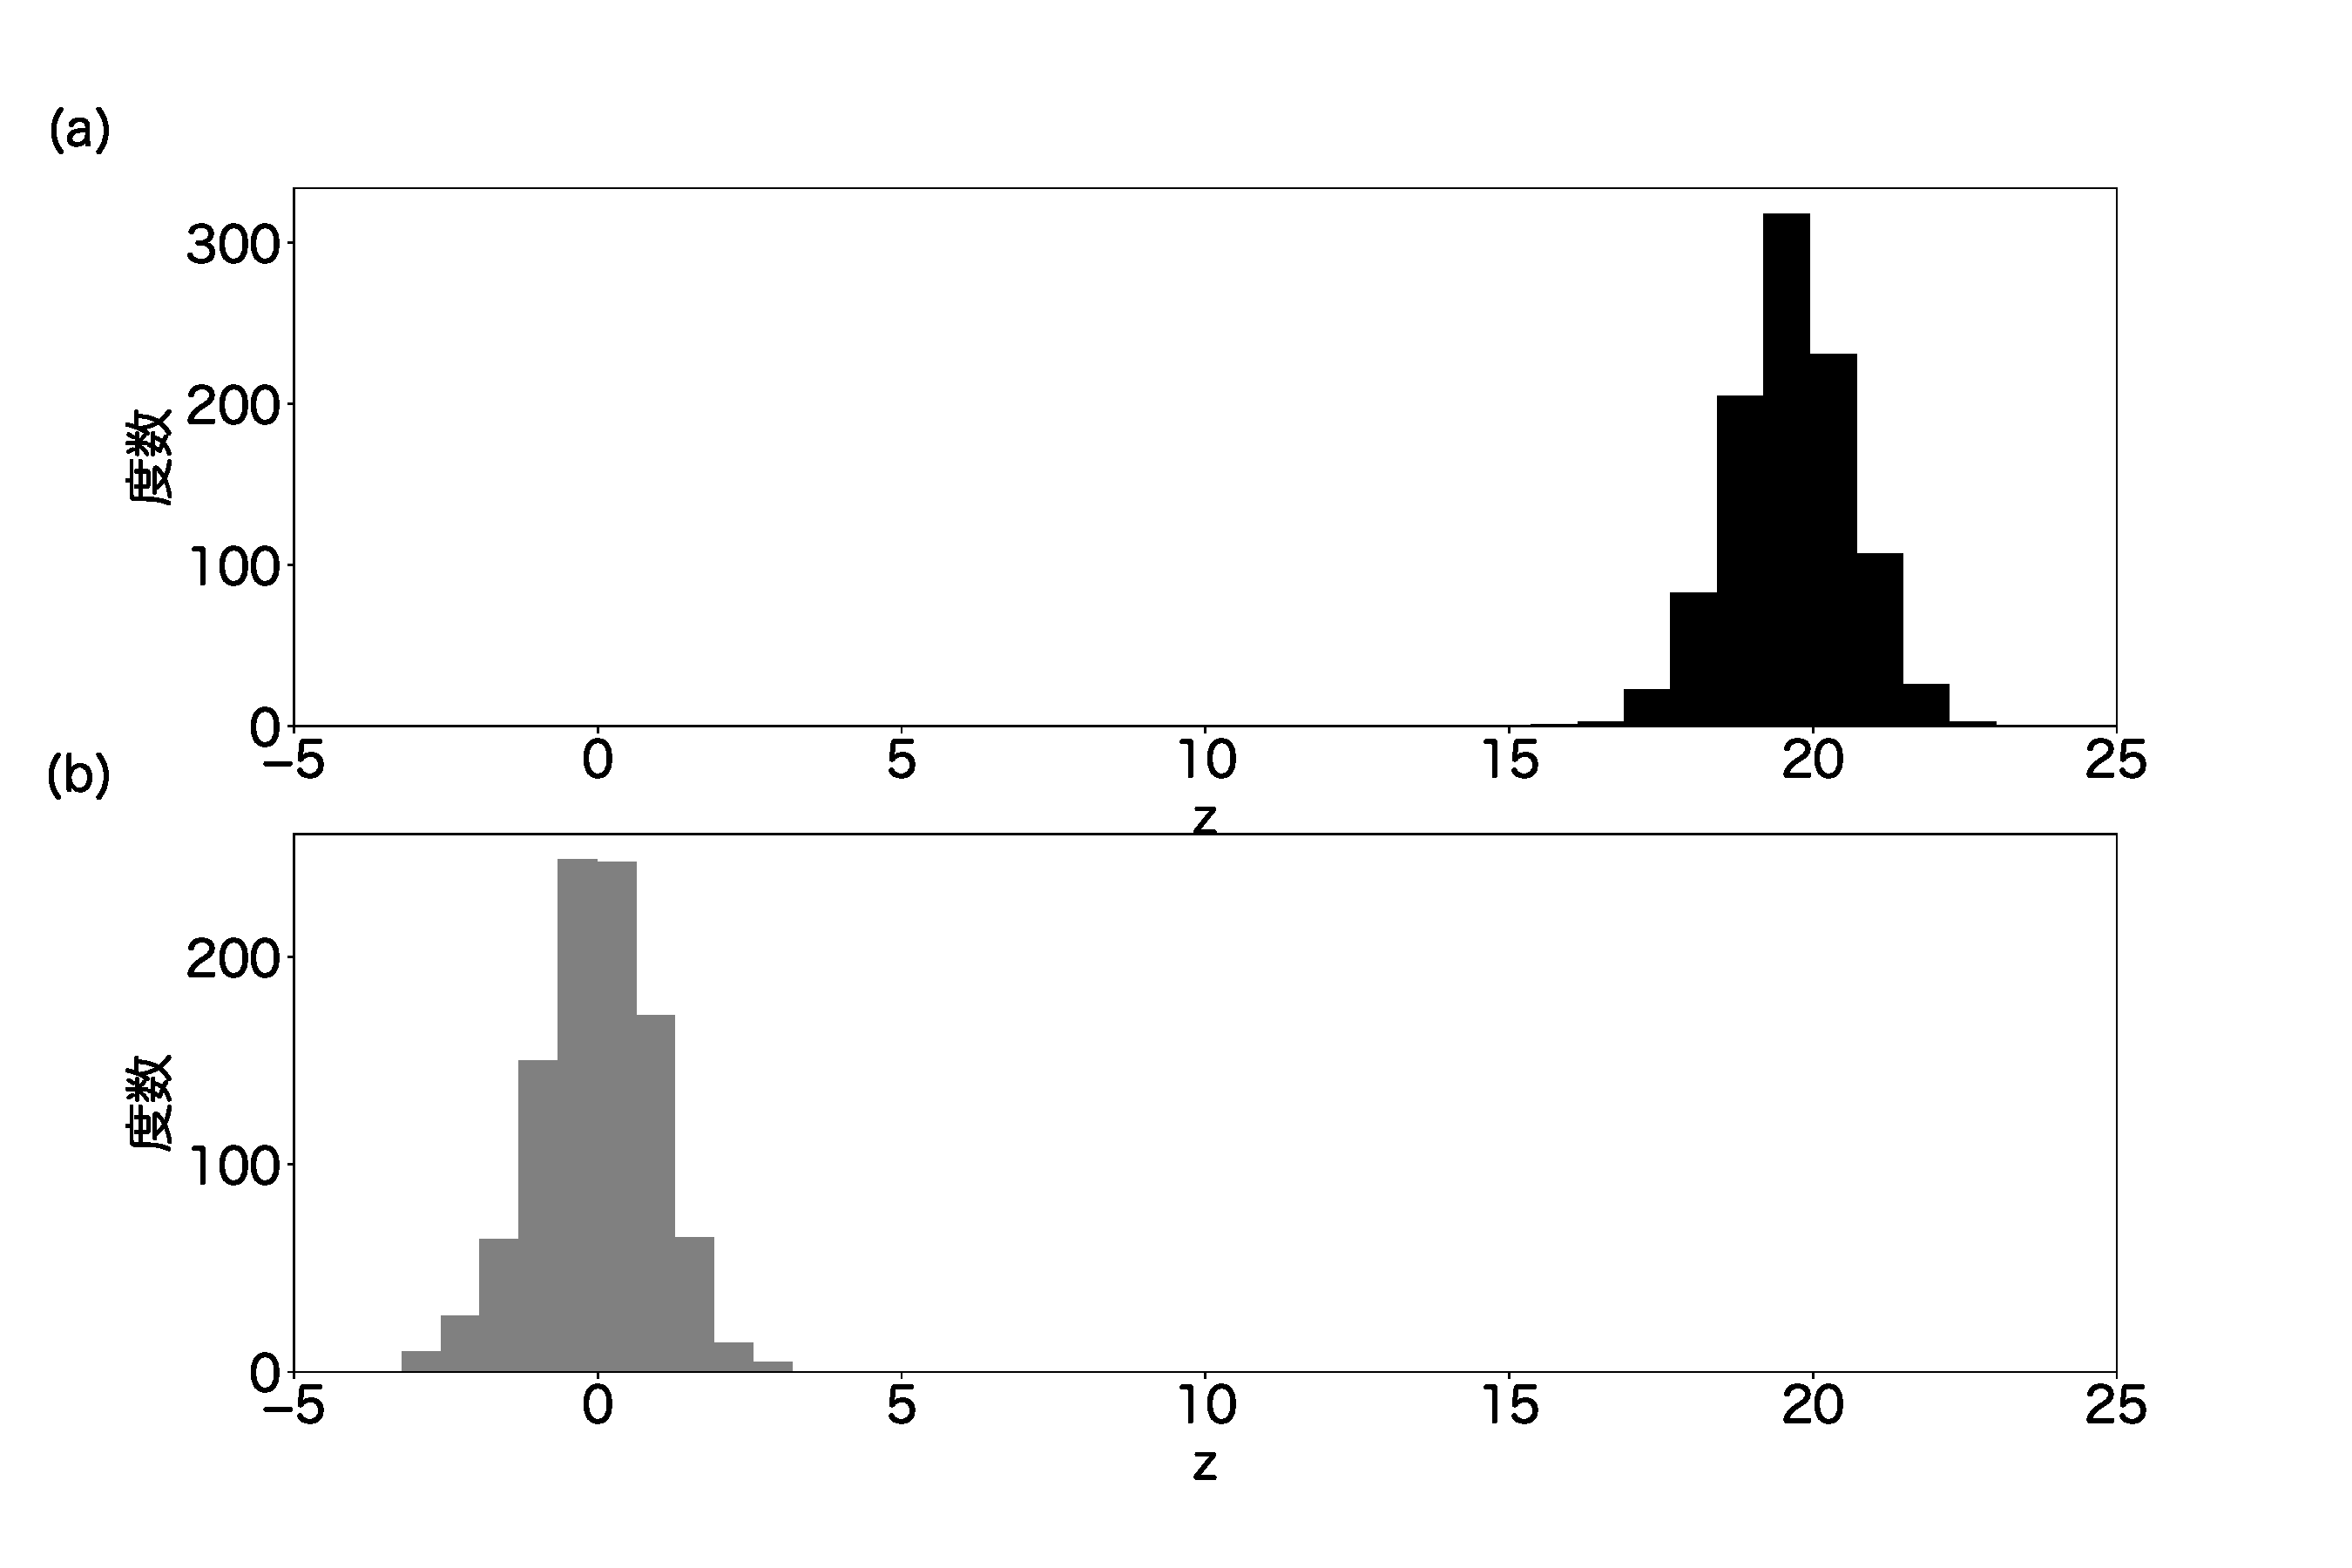
\includegraphics[width=15cm]{./image/02_/normal_distribution_test.pdf}
        \caption{(a)$N(1.96)$に従う確率変数を100個サンプリングし、その標本を1000個集めたときの$z=\sqrt{100}(\bar{X}-0)$のヒストグラム (b)$N(0,1)$に従う確率変数を100個サンプリングし、その標本を1000個集めたときの$z=\sqrt{100}(\bar{X}-0)$値のヒストグラム}
    \end{center}
\end{figure}


もう一つ例を挙げる。
$y_1,y_2,\cdots,y_n \sim N(170,5.8)$とする。このとき、この標本が$N(168,5.8)$によりサンプリングされたものではなくことを示すことはできるだろうか。
$z=\sqrt{n}\frac{\bar{y}-168}{\sigma}$を計算すればよい。
図には、$N(170,5.8)$に従う確率変数を100個サンプリングし、その標本を1000個集め、ヒストグラムを描いた。
これをみると、$0.5$を中心に分布が広がることがわかる。$z=\frac{\bar{X}-168}{\sqrt{\frac{5.8}{n}}}\sim N(0,1)$であるはずである。
複数回、標本を得た場合でも、$z$が$[-1.96,1.96]$の範囲に収まっている。このことは、$N(168,5.8)$ではないと判断できないことを示唆している。


\begin{figure}
    \begin{center}
        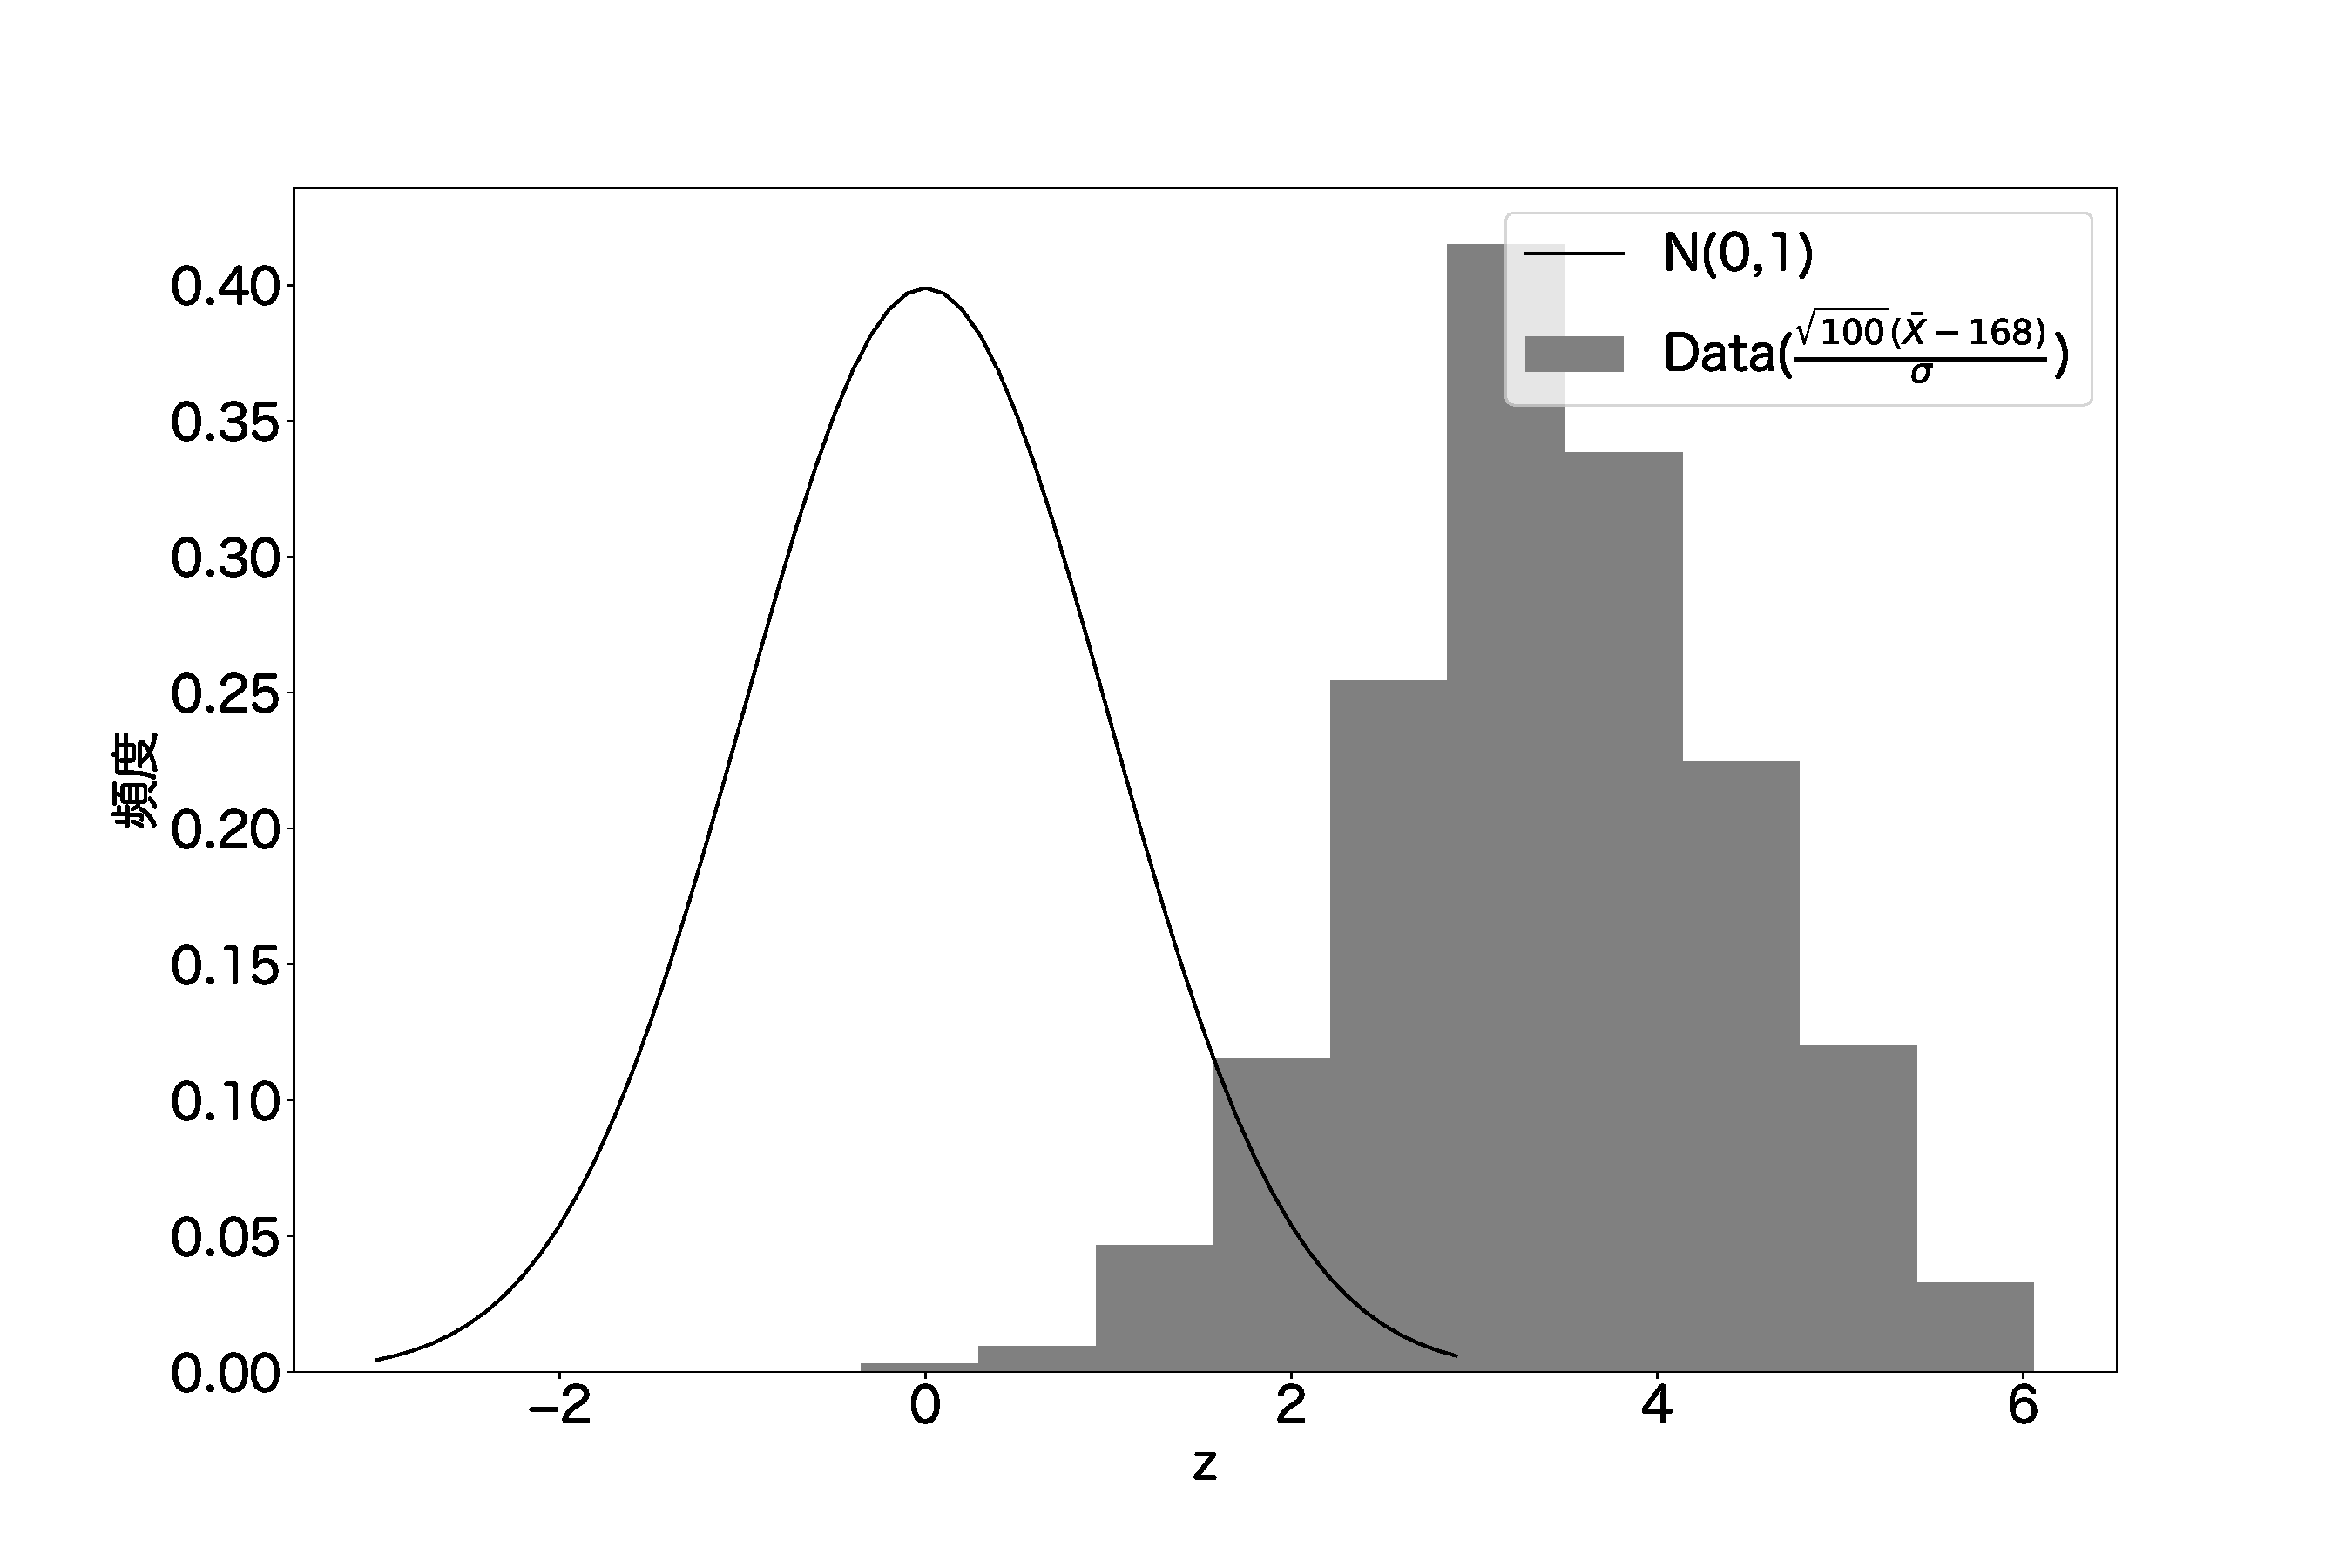
\includegraphics[width=15cm]{./image/02_/normal_distribution_test2.pdf}
        \caption{$N(170,5.8)$に従う確率変数を100個サンプリングし、その標本を1000個集めたときの$z=\sqrt{100}(\bar{X}-168)$のヒストグラム}
    \end{center}
\end{figure}


ある正規分布に従う確率変数$x_1,x_2,\cdots,x_n$が母数の異なる正規分布で得られる確率も計算できる。具体的には、$x_1,x_2,\cdots,x_n\sim N(\mu,\sigma^2)$とし、これが$N(\mu_1,\sigma_1^2)$で得られるとすると、そのときの統計量は、$z=\frac{\bar{x}-\mu_1}{\frac{\sigma_1}{n}}$である。この$z$は、$N(0,1)$に従うと考えられるので、$\phi(|z|>Z)$となる確率を計算すれば良い。

\begin{theo}
    確率変数$x_1,x_2,\cdots,x_n \sim N(\mu,\sigma^2)$ならば、$z=\frac{\bar{X}-\mu}{\sqrt{\frac{\sigma}{n}}} \sim N(0,1)$である。
    一方で、確率変数$x_1,x_2,\cdots,x_n \sim N(\mu,\sigma^2)$とする。$N(\mu_1,\sigma_1^2)$は正規分布とする。ただし、$\mu\neq \mu_1, \sigma =\sigma_1$このとき、$z=\frac{\bar{X}-\mu_1}{\sqrt{\frac{\sigma_1}{n}}} \sim N(0,1)$ではない。
\end{theo}
$\mu$と$ \mu_1$が極めて近い値のとき、$z=\frac{\bar{X}-\mu_1}{\sqrt{\frac{\sigma_1}{n}}} $も$N(0,1)$におけるよくある値になる言い換えれば、$\phi(|z|>Z)$は十分大きい。
一方で、$\mu$と$ \mu_1$が離れた値を取ると、$\phi(|z|>Z)$は小さな値になる。



\subsection{$(\star)$ $Exp(\lambda)$に従う確率変数であることを判定できるか}
$x_1,x_2,\cdots,x_n \sim Exp(\lambda)$であるとき、$n\bar{x}\sim Ga(n,\frac{1}{\lambda})$である。
母数不明の指数分布に従う確率変数が、$x_1,x_2,\cdots,x_n \sim Exp(\lambda)$と仮定したとき、$n\bar{x}\sim Ga(n,\frac{1}{\lambda})$でないならば、$x_1,x_2,\cdots,x_n \sim Exp(\lambda)$ではないと判断できるだろうか。シミュレーションによって確認してみよう。

この論法は、母数が不明の指数分布に従う確率変数を得たとき、その指数分布の母数が特定の値ではないことを示すためにこの論法を利用する。ここでは、母数が$\lambda=1,2,5,10,100$からサンプルサイズ4の標本を$1000$生成し、それら標本の統計量$n\bar{X}$のヒストグラムと、ガンマ関数$Ga(100,1)$の確率密度関数を比較する。

\begin{figure}
    \centering
    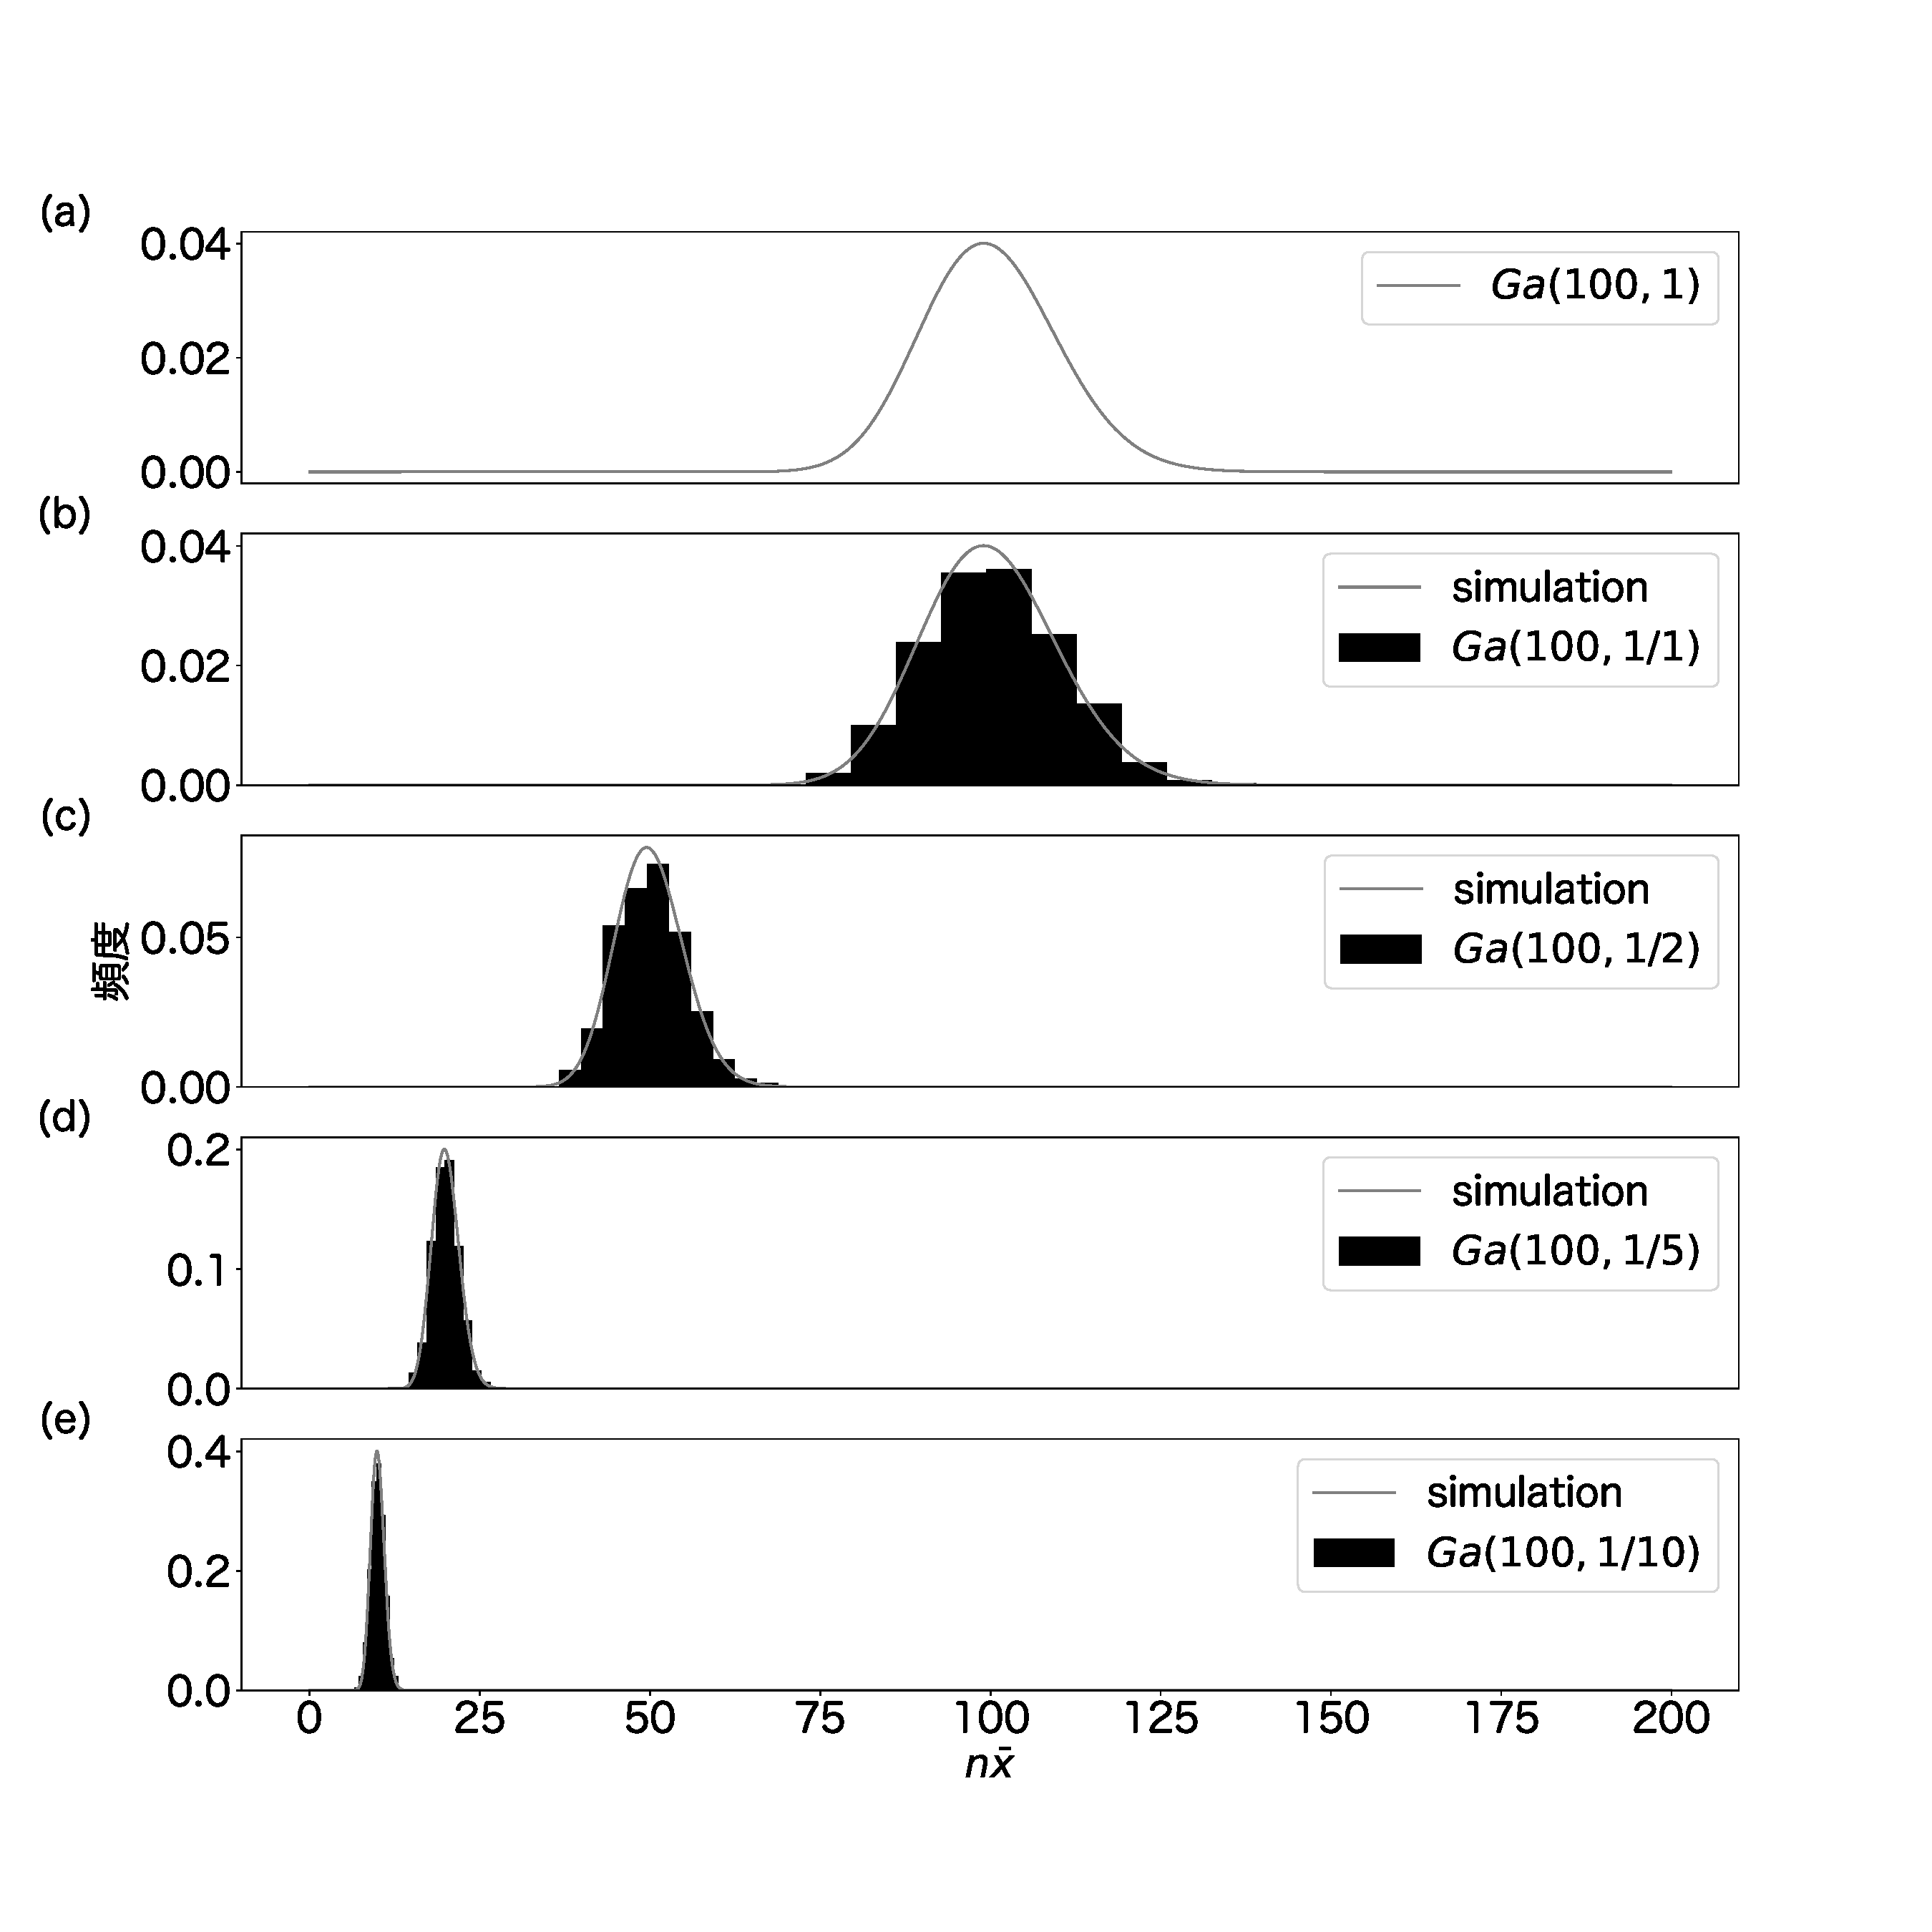
\includegraphics[width=15cm]{./image/02_/Exp_Gamma_simulation.pdf}
    \caption{(a)$Ga(10,1)$の確率密度関数。(b-e)指数分布からサンプルサイズ$4$の標本を$1000$回生成し、その統計量$n\bar{x}$のヒストグラム}
    \label{fig:exp_gamma_simulation}
\end{figure}

図\ref{fig:exp_gamma_simulation}(a)は、指数分布$Exp(\lambda=1)$の確率密度関数を示している。
図\ref{fig:exp_gamma_simulation}b-eは、シミュレーションの結果を示している。
図\ref{fig:exp_gamma_simulation}(b)には、指数分布$Exp(1)$に従う確率変数の統計量$n\bar{x}$が確かに、$Ga(100,1)$に従うことが確かめれる。
図\ref{fig:exp_gamma_simulation}(c-e)では、指数分布の$\lambda$が$1/2,1/5,1/10$のときの統計量のヒストグラムである。これらと、図\ref{fig:exp_gamma_simulation}(a)を比較すると、分布が異なっているので、確かに、$Ga(100,1)$には従わないことがわかる。



\subsection{TEST}

これらの事象は、統計モデルの上で観測される、数学的な事実です。
数学を扱っている以上はこの事実は決して崩れることはありえません。
一方で、我々が扱う現象ではどうなるでしょうか。現象が数学な分布関数から生成されていることは決してありえません。
誰かがサイコロを振って、人々の身長を決めているのなら話は別ですが、
人の身長が、ランダムに正規分布によって決定されることはありませんね。

$M(168)$モデルの平均値は$168cm$、データでは$171cm$程度なので、$3cm$小さい。また、
$180cm$以上の人の割合を使ってモデルとデータの乖離を調べることができました。
$180cm$の人がたまたまいなかった場合は、$M(169.1),M(168)$のどちらも推測できているとは言い難いことになります。このことから、特定の値を使って乖離を判定することは難しいと考えられます。


$\phi(z>Z(\mu))を$p値として、絶対に選択してはいけない統計モデル$M(\mu)$の母数$\mu$を調べます。具体的には、指標$p$が$0.05$より小さい統計モデルを選択しないようにします。その母数の範囲は$162.14 >\mu, \mu > 174.31$です。この母数の統計モデルは$p=0.05$の基準で使わないことを統計モデルを棄却すると言います。逆に、$p>0.05$となるモデルは、積極的に正しいとは考えません。明らかに間違いではないけども正しくもないという判断をします。


$p$値を使う方法がとられます。p値とは統計モデルとデータの乖離度合いを示す指標です。p値は$0~1$の値をとり、$0$に近いと統計モデルとデータが乖離していると判断します。




\section{04}
\subsubsection{いつでも正規モデルでいこう}
データが非対称に分布しているのに、統計モデルに正規分布を指定した場合、推定が正しく行えないことを確認しておこう\footnote{元ネタ。
    小標本 t 検定の誤解:中心極限定理と一般化線形モデル 井口豊(生物科学研究所,長野県岡谷市)\url{https://biolab.sakura.ne.jp/small-sample-t-test-glm.html}}。
次のような統計モデルを構築する。
\begin{enumerate}
    \item $X_1,X_2,\cdots,X_n $はi.i.d
    \item 正規分布
    \item 正規分布の母数$\mu$,$\sigma^2$の値は不明
\end{enumerate}
正規分布の母数$\mu=1$とした統計モデルを$M(1)$と記述する。
この$X_1,X_2,\cdots,X_n$について次の統計量が$t(n)$分布に従うことがわかっている。
\begin{equation*}
    T = \frac{\bar{X}-1}{\sqrt{\frac{\sigma^2}{n}}} \sim t(n)
\end{equation*}
このとき、データが、既知の確率分布から得られた場合に、$p$値がサンプルサイズによってどのように変化するのかを調べる。
具体的に、平均$1$の指数分布または、平均$1$、標準偏差$1$の正規分布からサンプルを得て標本を作る。その標本を$100000$回取得する。
このとき、$T$値を計算し、$T$値いじょの値が得られる確率$p$を計算する。その$p$が$p<0.05$となる割合を計算する。以上をサンプルサイズを変化させてシミュレーションを行なった。

平均$1$、標準偏差$1$の正規分布の場合、統計モデルの仮定と一致するので、$T$値は$t(n)$分布に従う。よって、$p<0.05$となる頻度も、$5\%$程度になることが期待される。
一方で、平均$1$の指数分布の場合、統計モデルの仮定と一致しない。このことから、$T$は$t(n)$分布に従うとはいえない。このことから、$p<0.05$となる頻度はわからない。


\begin{figure}
    \begin{center}
        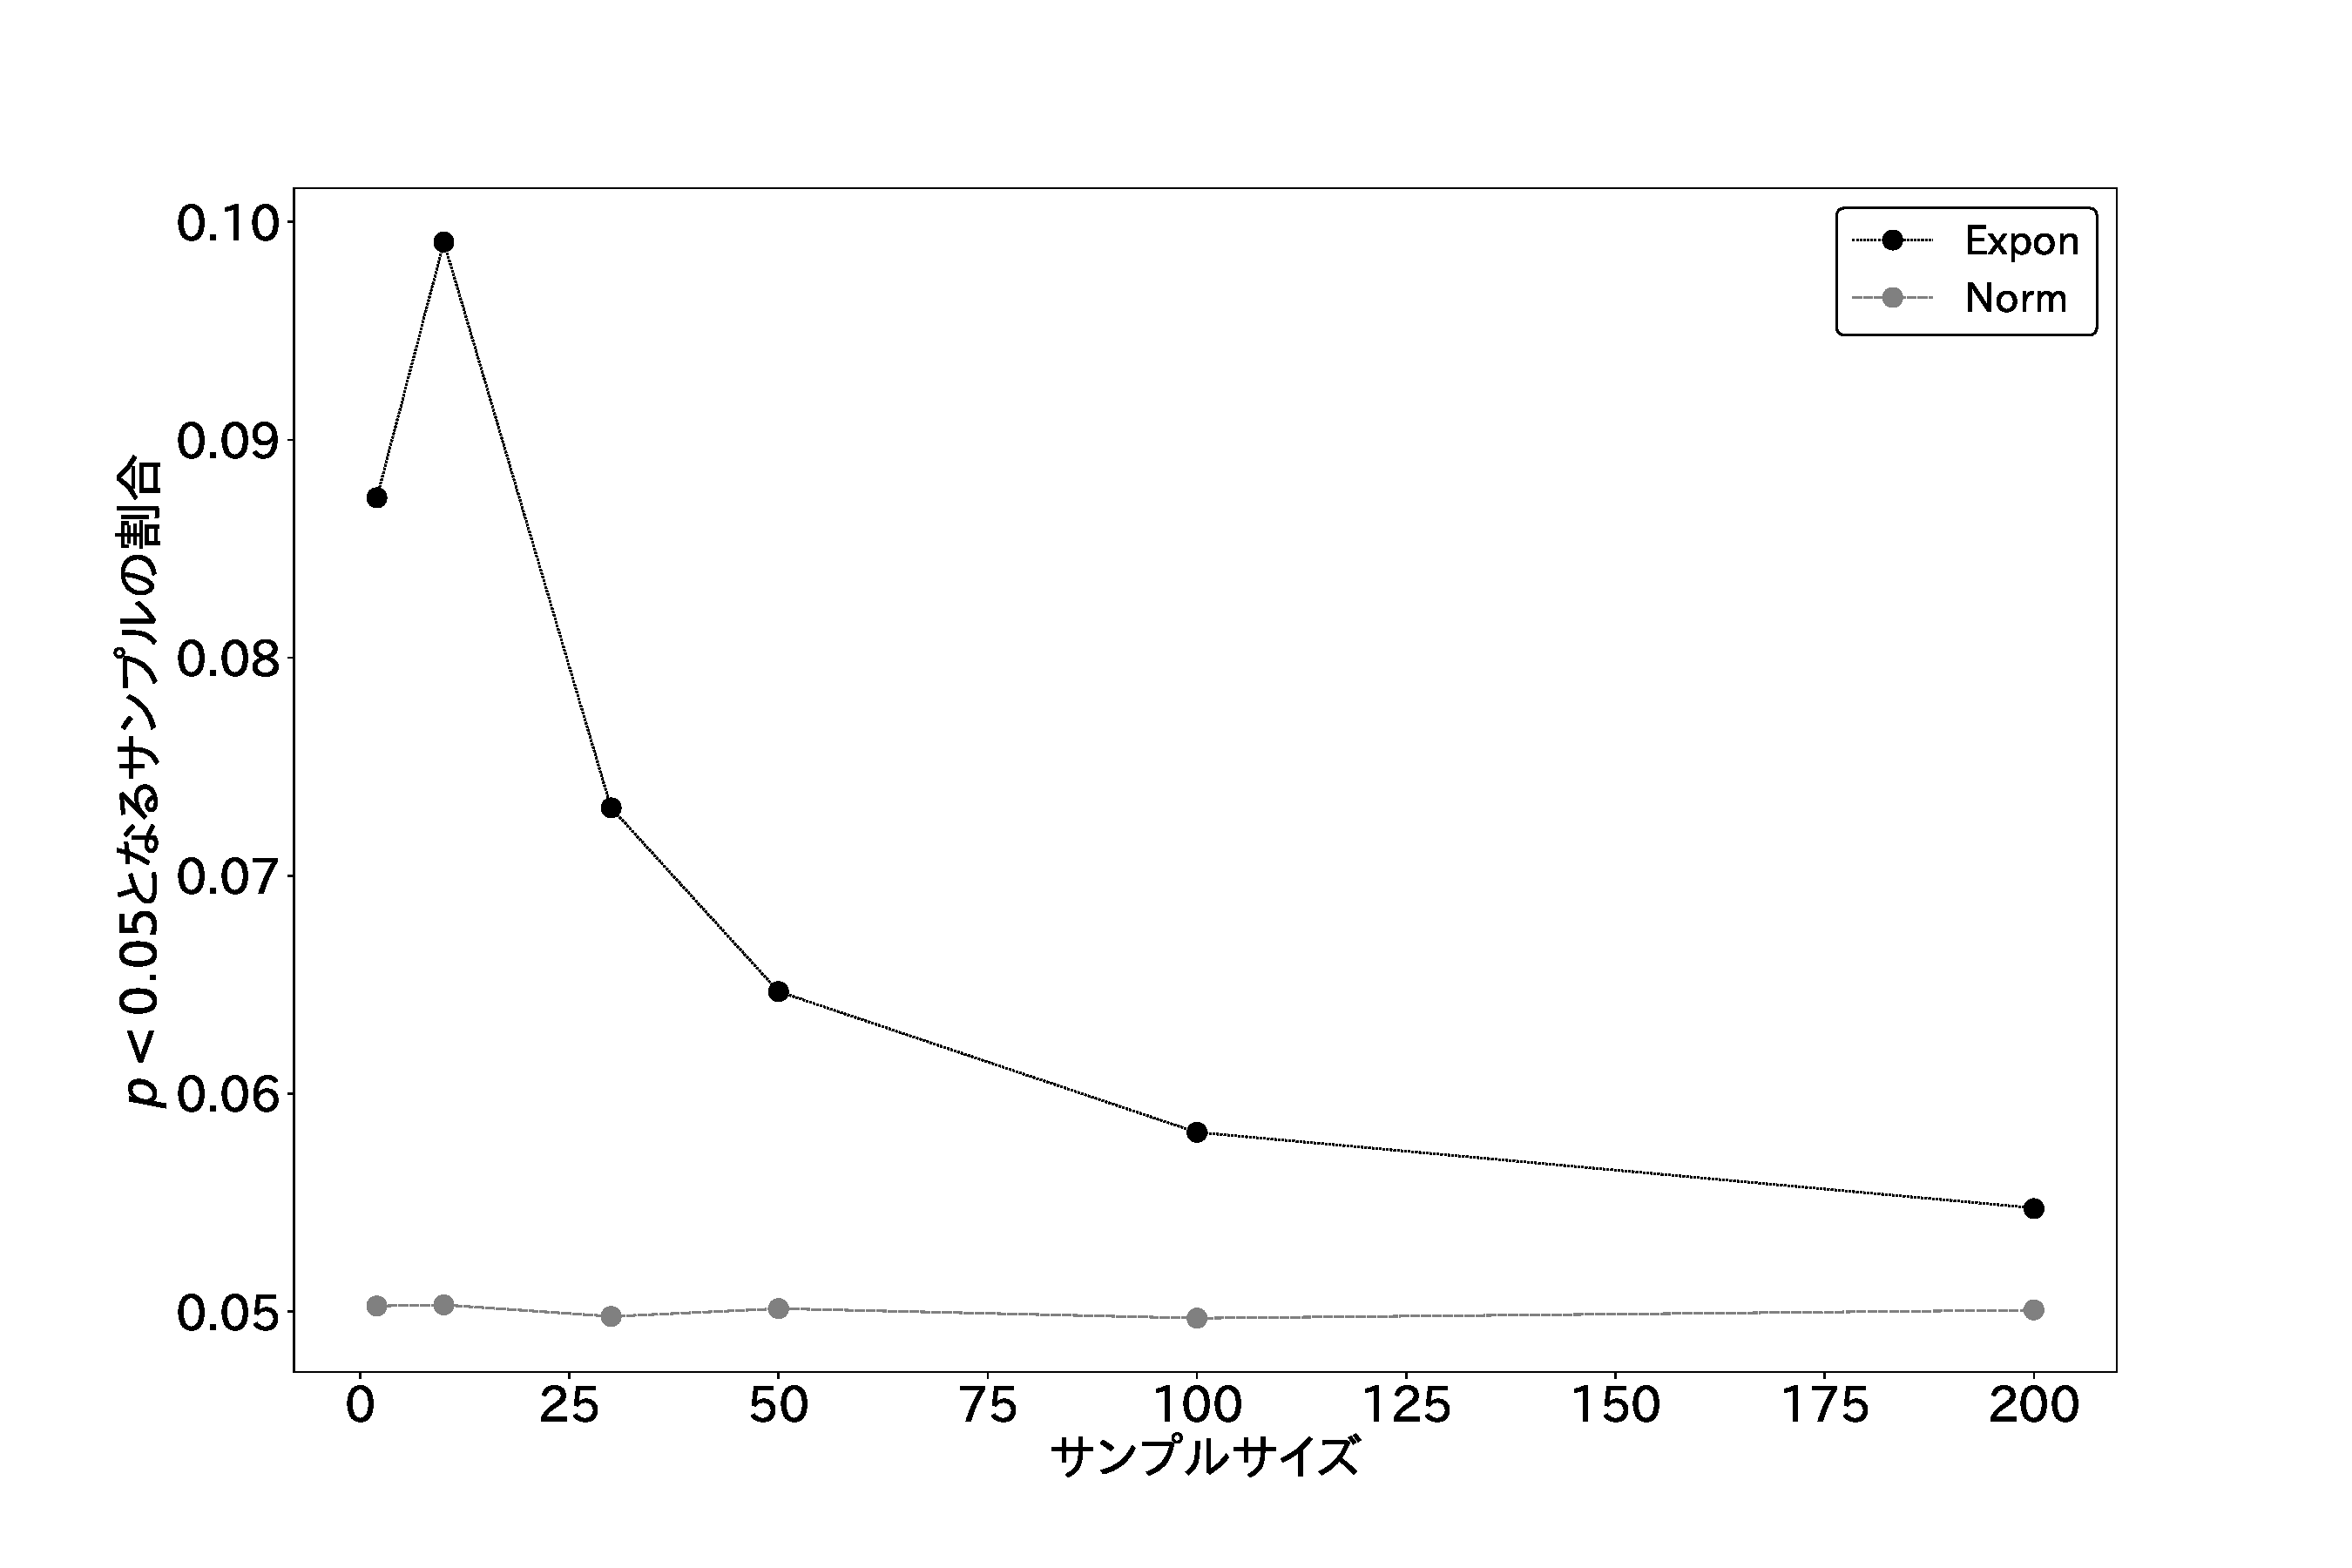
\includegraphics[width=15cm]{./image/04_/t_test_expon_norm.pdf}
        \caption{正規分布または指数ぶんぷから得た標本の$T$値から計算した$p$値で、$p<0.05$以下になる割合}
    \end{center}
\end{figure}

シミュレーションの結果、正規分布から標本を得た場合、$p<0.05$になる割合は、サンプルサイズに依存せず、$5\%$程度であり、理論と一致する。
一方で、指数分布から標本を得た場合、$p<0.05$になる割合はサンプルサイズに応じて変化しており、また、どのサンプルサイズでも$p<0.05$となる割合は$5\%$より多い。
このように、データが正規分布とかけ離れているにもかかわらず、正規モデルを構築し、そこから統計量を計算しても、的外れになることがあることを示唆している\footnote{$n$を大きくしたとき、中心極限定理より、$p<0.05$となる割合も$5\%$に近づくと解釈することがある。本当だろうか。具体的には、次の定理が成り立つのだろうか。
\begin{quote}
\begin{theo}
    $X_1,X_2,\cdots,X_n \sim Exp(\lambda)$とするとき、$T=\frac{\bar{X}-1/\lambda}{\sqrt{\frac{S^2}{n}}}$ここで、$S^2=\frac{1}{n-1}\sum_{i=1}^n(X_i-\bar{X})^2$である。$T\sim t(n-1)$または、$t$がなんらかの統計分布に従う。または、$E[T]<\infty,Var[T]<\infty$
\end{theo}
\end{quote}
このことが成り立つなら、中心極限定理も成立し、$n$が十分大きいときに、分布関数を近似できそうである。
}


\section{12}
\subsection{a}
このモデルにおいて、統計量$Z(\bar{x},\mu)$の$95\%$予測区間を求める。
%よく入る区間の式を変形し、データを得たときに、そのデータを基準にした$\mu$の範囲に変形してみます。
\begin{eqnarray*}
 & -z_{0.025} < Z(\bar{x},\mu)<z_{0.025} \\
\rightarrow & -z_{0.025} < \frac{\sqrt{n}(\bar{x}-\mu)}{\sigma}  <z_{0.025} \\
\rightarrow & \bar{x}- z_{0.025}\frac{\sigma}{\sqrt{n}} < \mu < \bar{x} + z_{0.025}\frac{\sigma}{\sqrt{n}}
\end{eqnarray*}


を使い、最尤モデルにおける平均値は、
$\bar{x}\sim N(\mu_{ML},\sigma^2_{ML}/\sqrt{n})$である。
このことから、モデルは、$\left[ \mu_{ML}-z_{0.05}\sigma_{ML},\mu_{ML}+z_{0.05}\sigma_{ML} \right]$
の間に、$68\%$の確率で平均値が入ることを予測する。


\begin{framed}
    まとめ、
    \begin{itemize}
        \item 統計モデル$M(\mu)$によってサンプリングし、標本を得たとき、標本平均値のよくある値の範囲が信頼区間
    \end{itemize}
    \end{framed}



    標本では、$168.9 < \mu < 176.0$、
この範囲にある$\mu$をもつ統計モデルであれば、この標本によって棄却されない。
%標本$2$では、$165.5 < \mu <172.6$です。
例えば、このモデル$M(\bar{x})$の信頼区間であれば、$M(168)$は棄却できない。




まとめ、
\begin{framed}
    \begin{itemize}
        \item 統計モデル$M(\mu)$のサンプルの平均が$95\%$の確率で入る範囲$\mu - z_{0.025} \frac{\sigma}{\sqrt{n}} < \bar{X} < \mu + z_{0.025} \frac{\sigma}{\sqrt{n}}$。現実の母集団が統計モデルによってよく推測できるなら、この範囲に平均値が入る確率は$95\%$に近くなることもある。逆に、統計モデルが現実をよく捉えることができなければ、母集団から無作為抽出した標本の平均値はこの範囲に入ることは少なくなる。
        \item データがよくある範囲に入る統計モデル$M(\mu)$の$\mu$の範囲$\bar{x}- z_{0.025}\frac{\sigma}{\sqrt{n}} < \mu < \bar{x} + z_{0.025}\frac{\sigma}{\sqrt{n}}$
        \item  統計モデル$M(\mu)$ではサンプルサイズを大きくすると、平均値が入る範囲が狭くなる。
    \end{itemize}
\end{framed}


複数の確率変数$x_1,x_2,\cdots,x_n$が$N(\mu,\sigma^2)$に従わないことを推定したい。

サンプルサイズが大きいときは、最尤推定を行い、$\mu_1=\bar{x},\sigma_1^2=\sum_{i=1}^{n} (x_i-\bar{x})^2/n$を計算し、その値が、$\mu,\sigma^2$と著しく異なっていれば、$N(\mu,\sigma^2)$に従わないと言えそうである。
例えば、図\ref{fig:maximum_likelihood_0}は、正規分布$N(170,6.8^2)$からサンプルサイズ$100$の標本を得たとき、図\ref{fig:maximum_likelihood_1}は、サンプルサイズ$30$、そしてそのデータの分布と、最尤推定量から予測されるも確率密度関数、$N(168,6.8^2),N(171,6.8^2)$を表している。図\ref{fig:maximum_likelihood_0}をみると、最尤推定した確率密度関数がデータの出現頻度をよく表していること、そして、周辺の二つの正規分布$N(168,6.8^2),N(171,6.8^2)$とデータが乖離していることがわかる。
一方、図\ref{fig:maximum_likelihood_1}では、データが$N(171,6.8^2)$に従っているのではないかという疑惑が残る。

\begin{figure}
    \begin{center}
        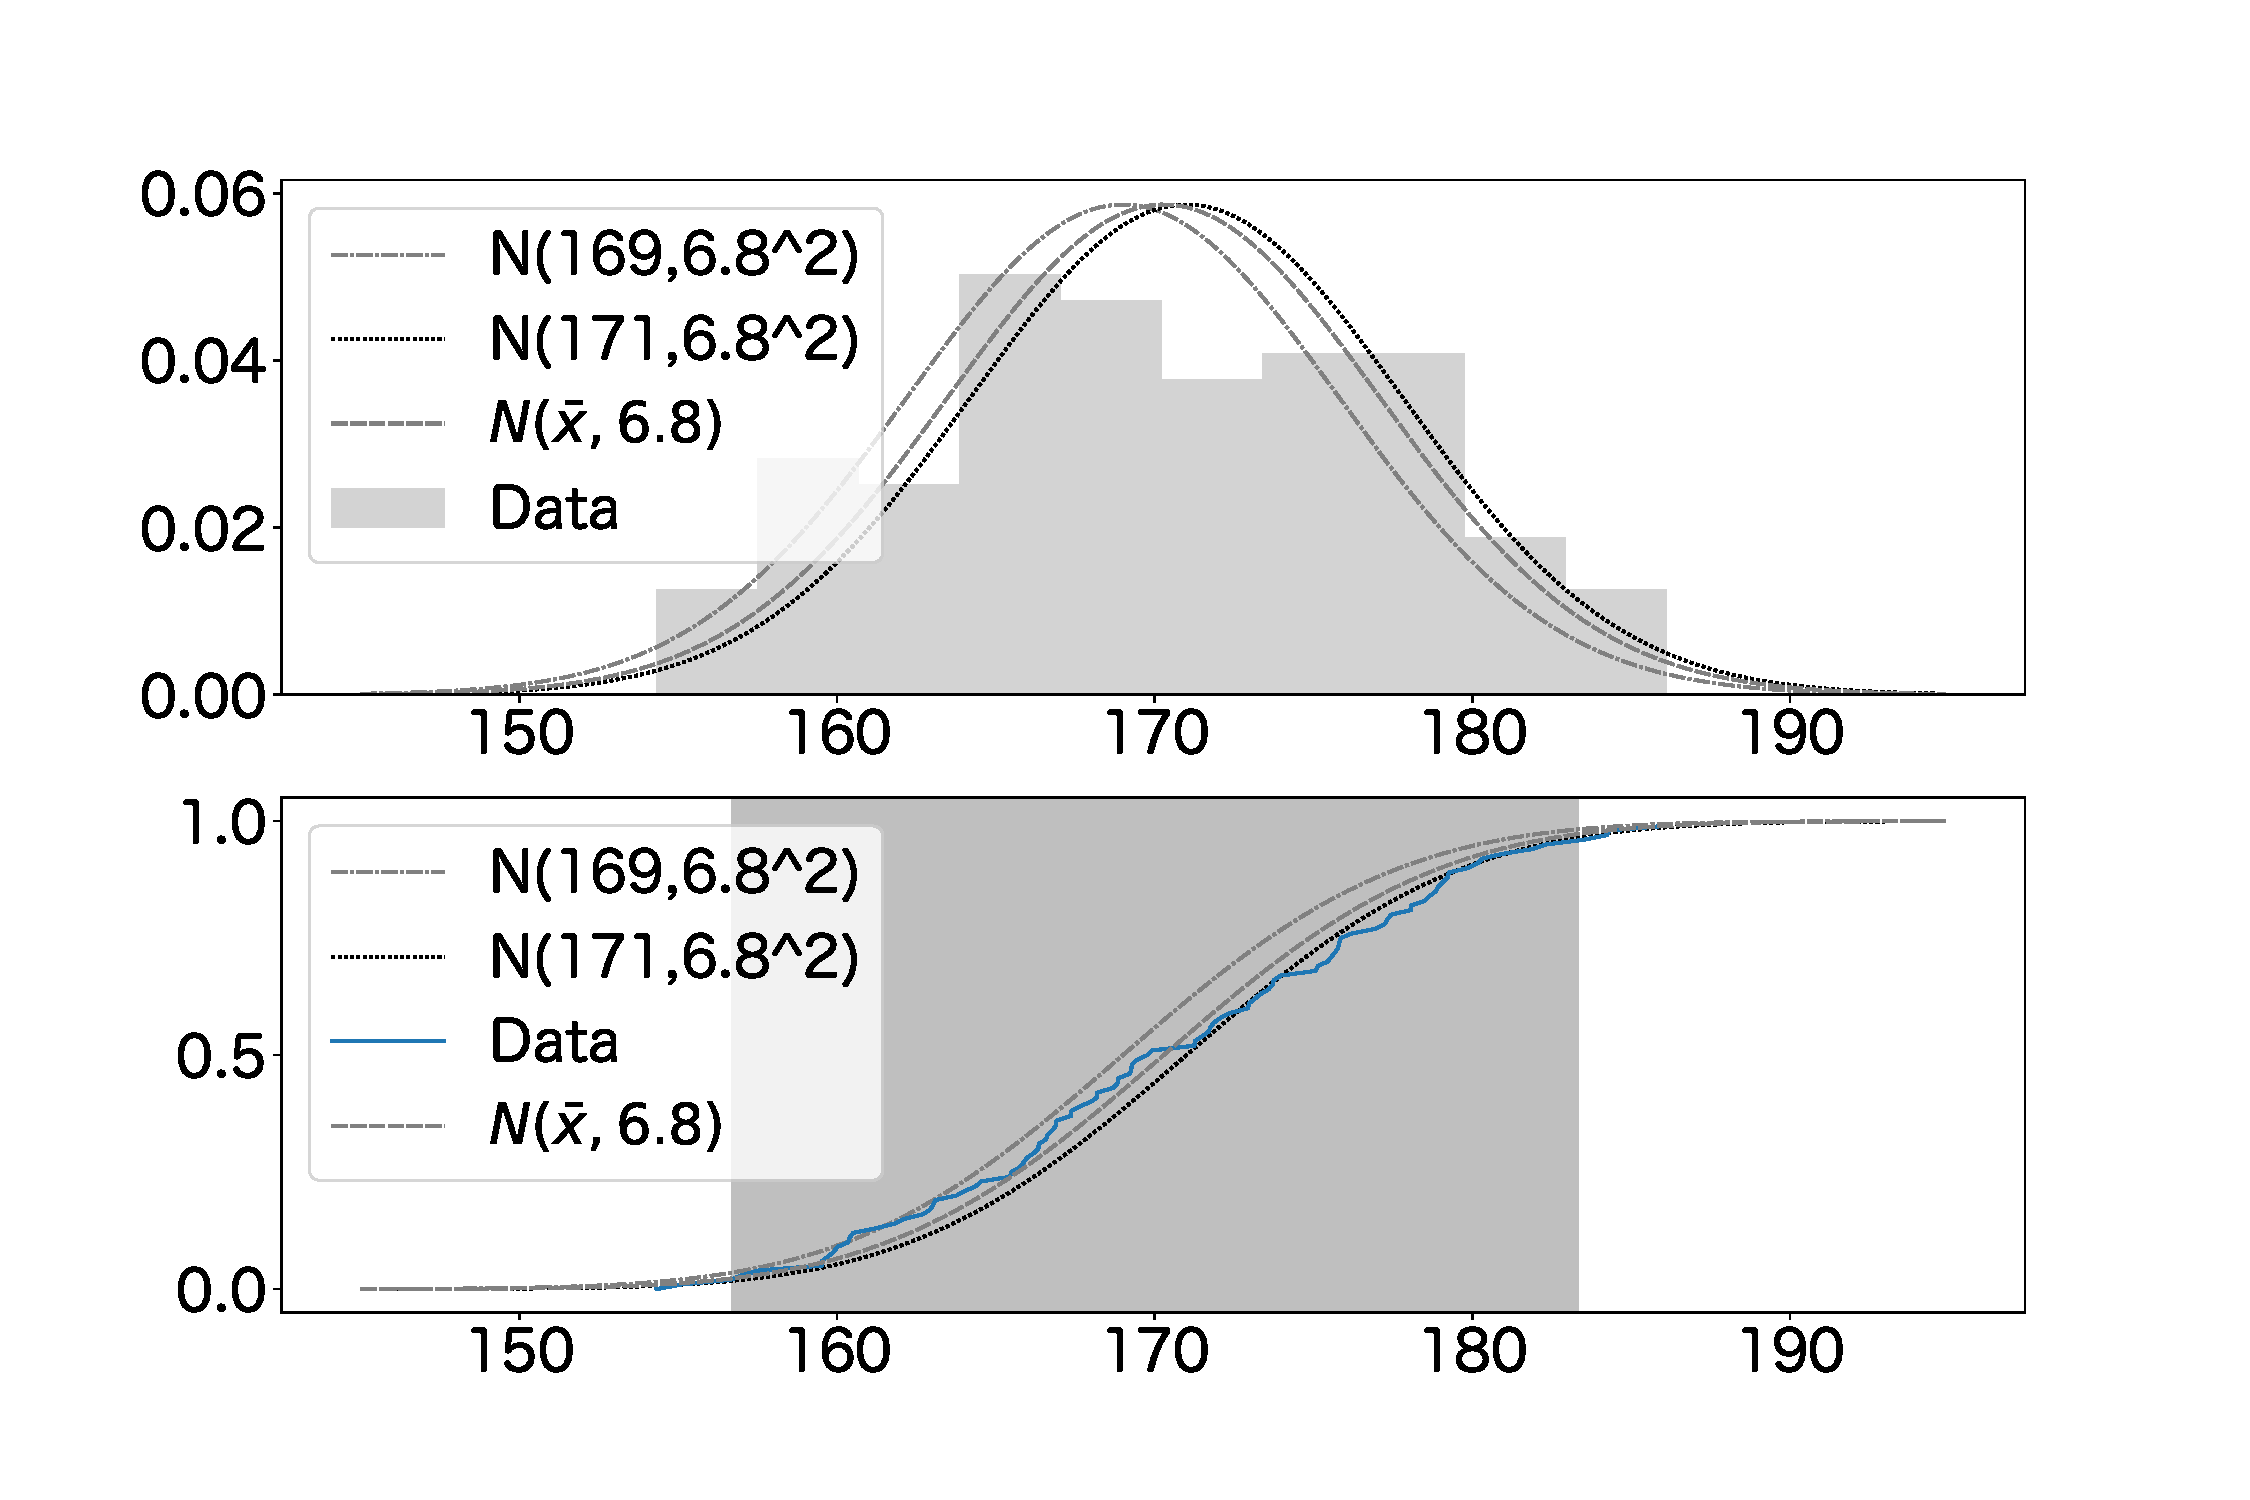
\includegraphics[width=15cm]{./image/02_/maximum_likelihood_0.pdf}
        \caption{$N(170,6.8^2)$からサンプルサイズ$100$の標本を得たときの分布。その最尤推定量により求められる分布関数。$N(168,6.8^2),N(171,6.8^2)$の分布関数を示す}
        \label{fig:maximum_likelihood_0}
    \end{center}
\end{figure}
\begin{figure}
    \begin{center}
        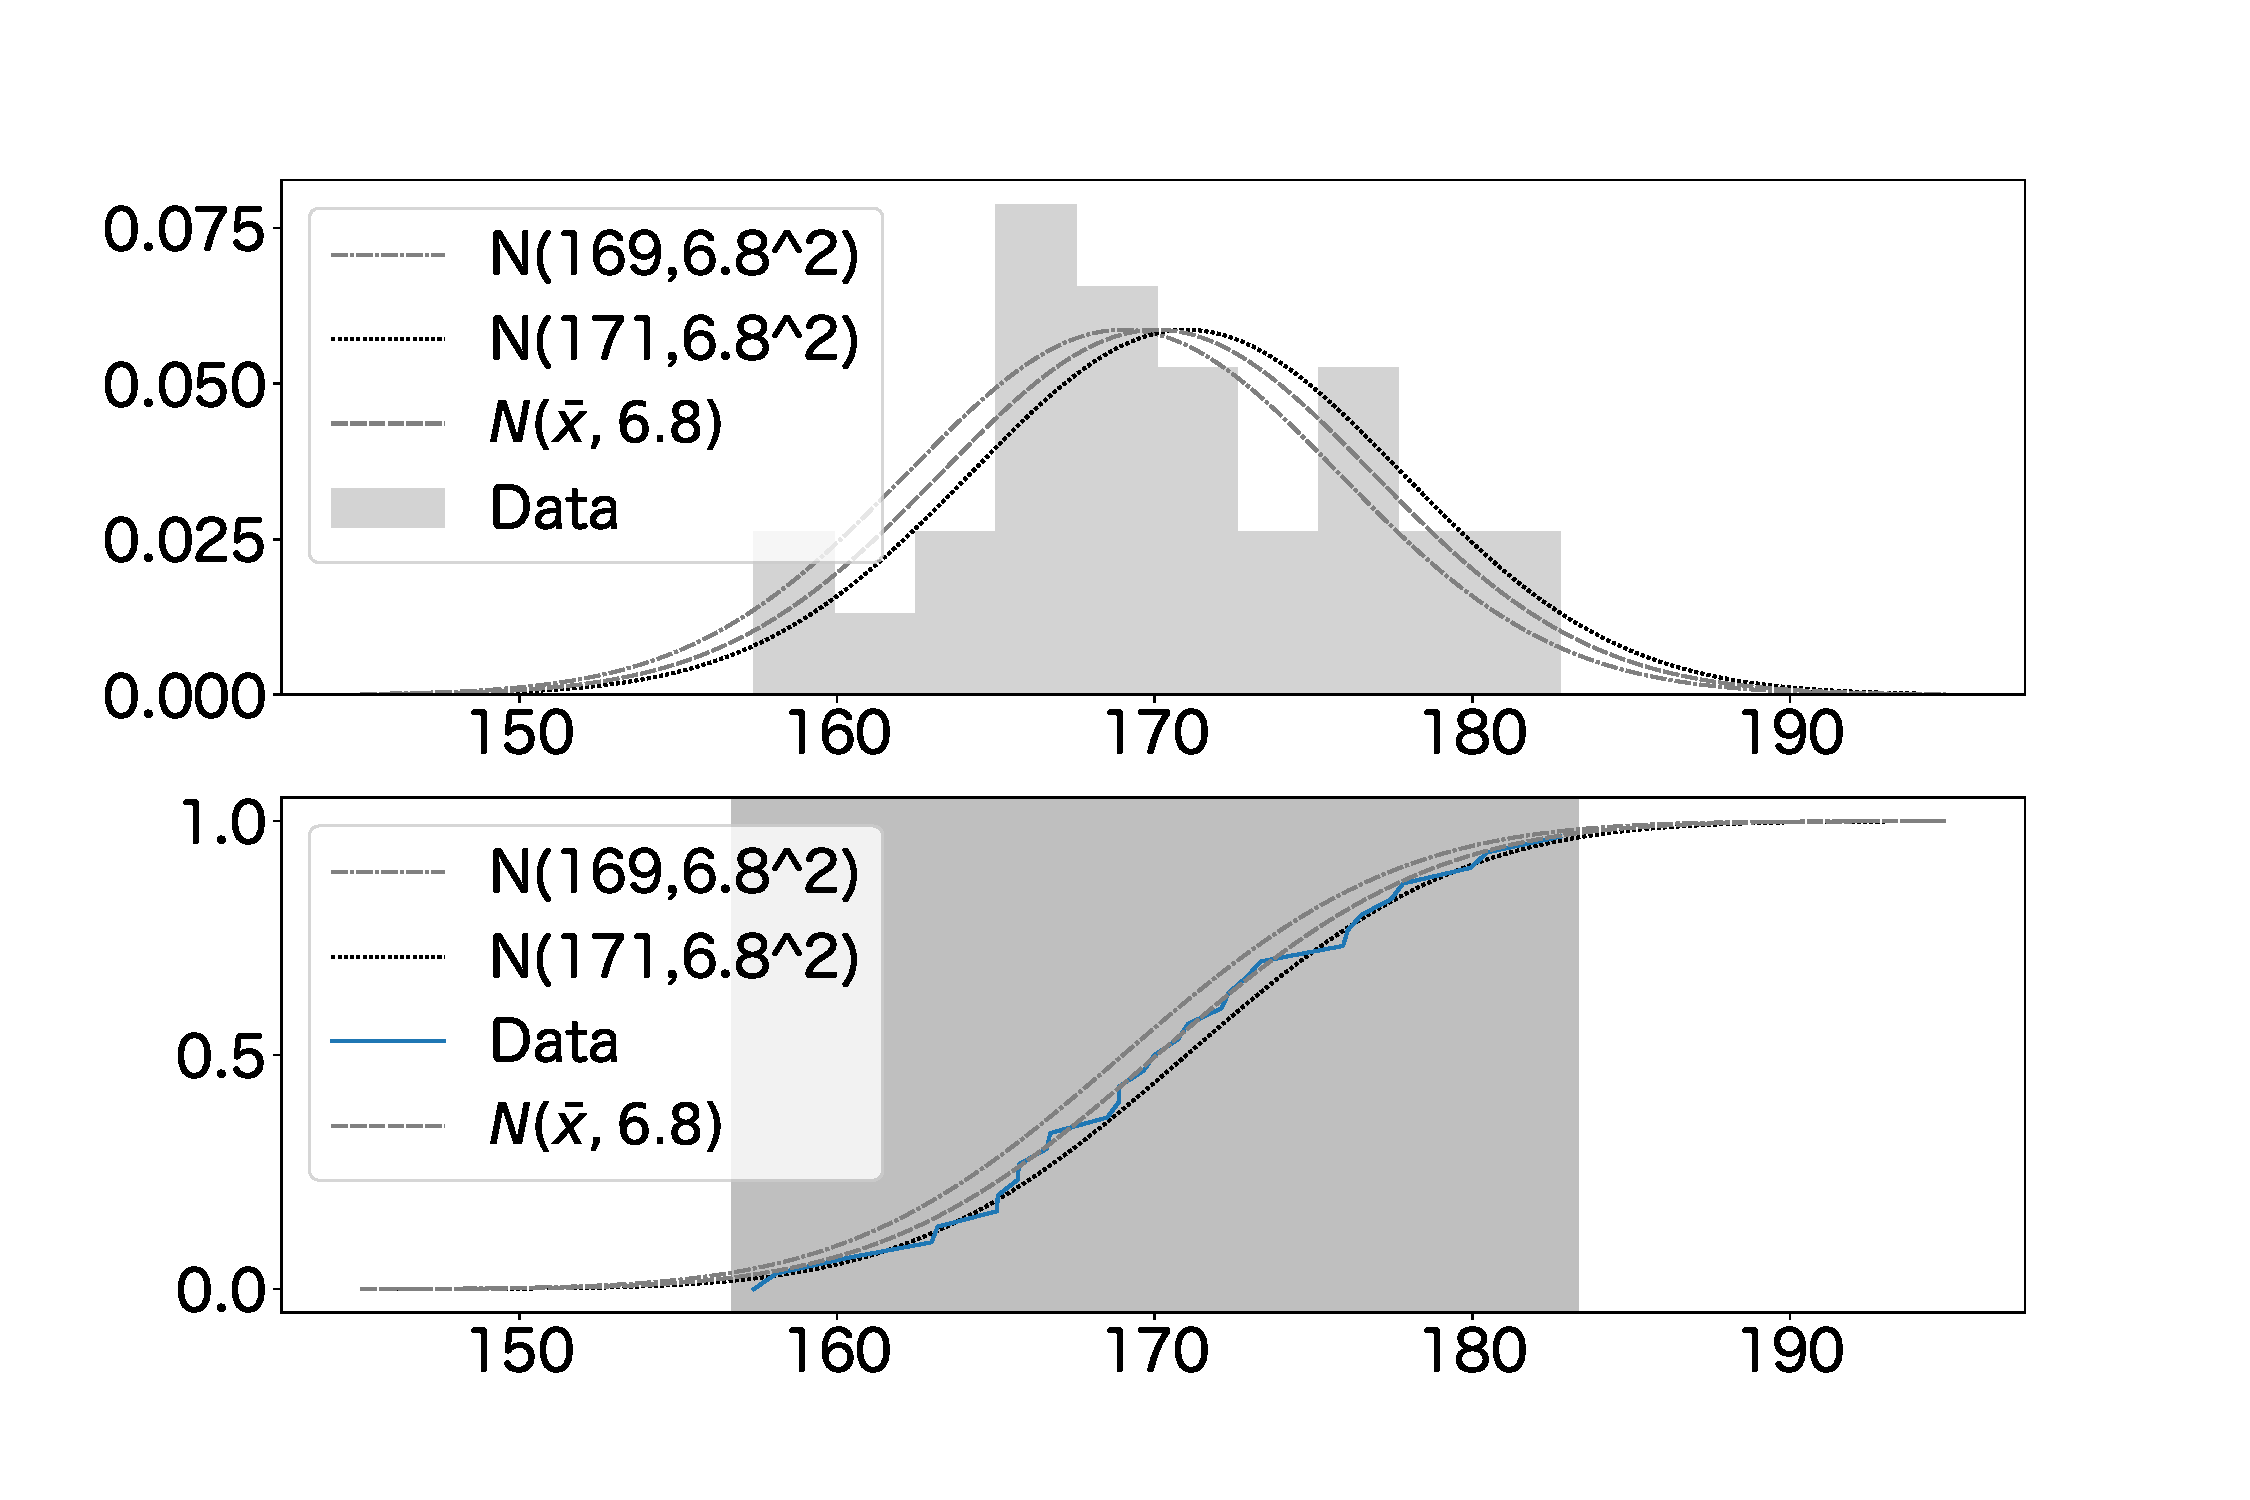
\includegraphics[width=15cm]{./image/02_/maximum_likelihood_1.pdf}
        \caption{$N(170,6.8^2)$からサンプルサイズ$30$の標本を得たときの分布。その最尤推定量により求められる分布関数。$N(168,6.8^2),N(171,6.8^2)$の分布関数を示す}
        \label{fig:maximum_likelihood_1}
    \end{center}
\end{figure}

このように、サンプルサイズが大きいと、最尤推定により推測した確率密度関数を見れば、そのほかの母数に従わないことがわかる場合がある。
また、より近くにある母数の確率密度関数と区別することは難しいこともわかる。

\begin{figure}
    \begin{center}
        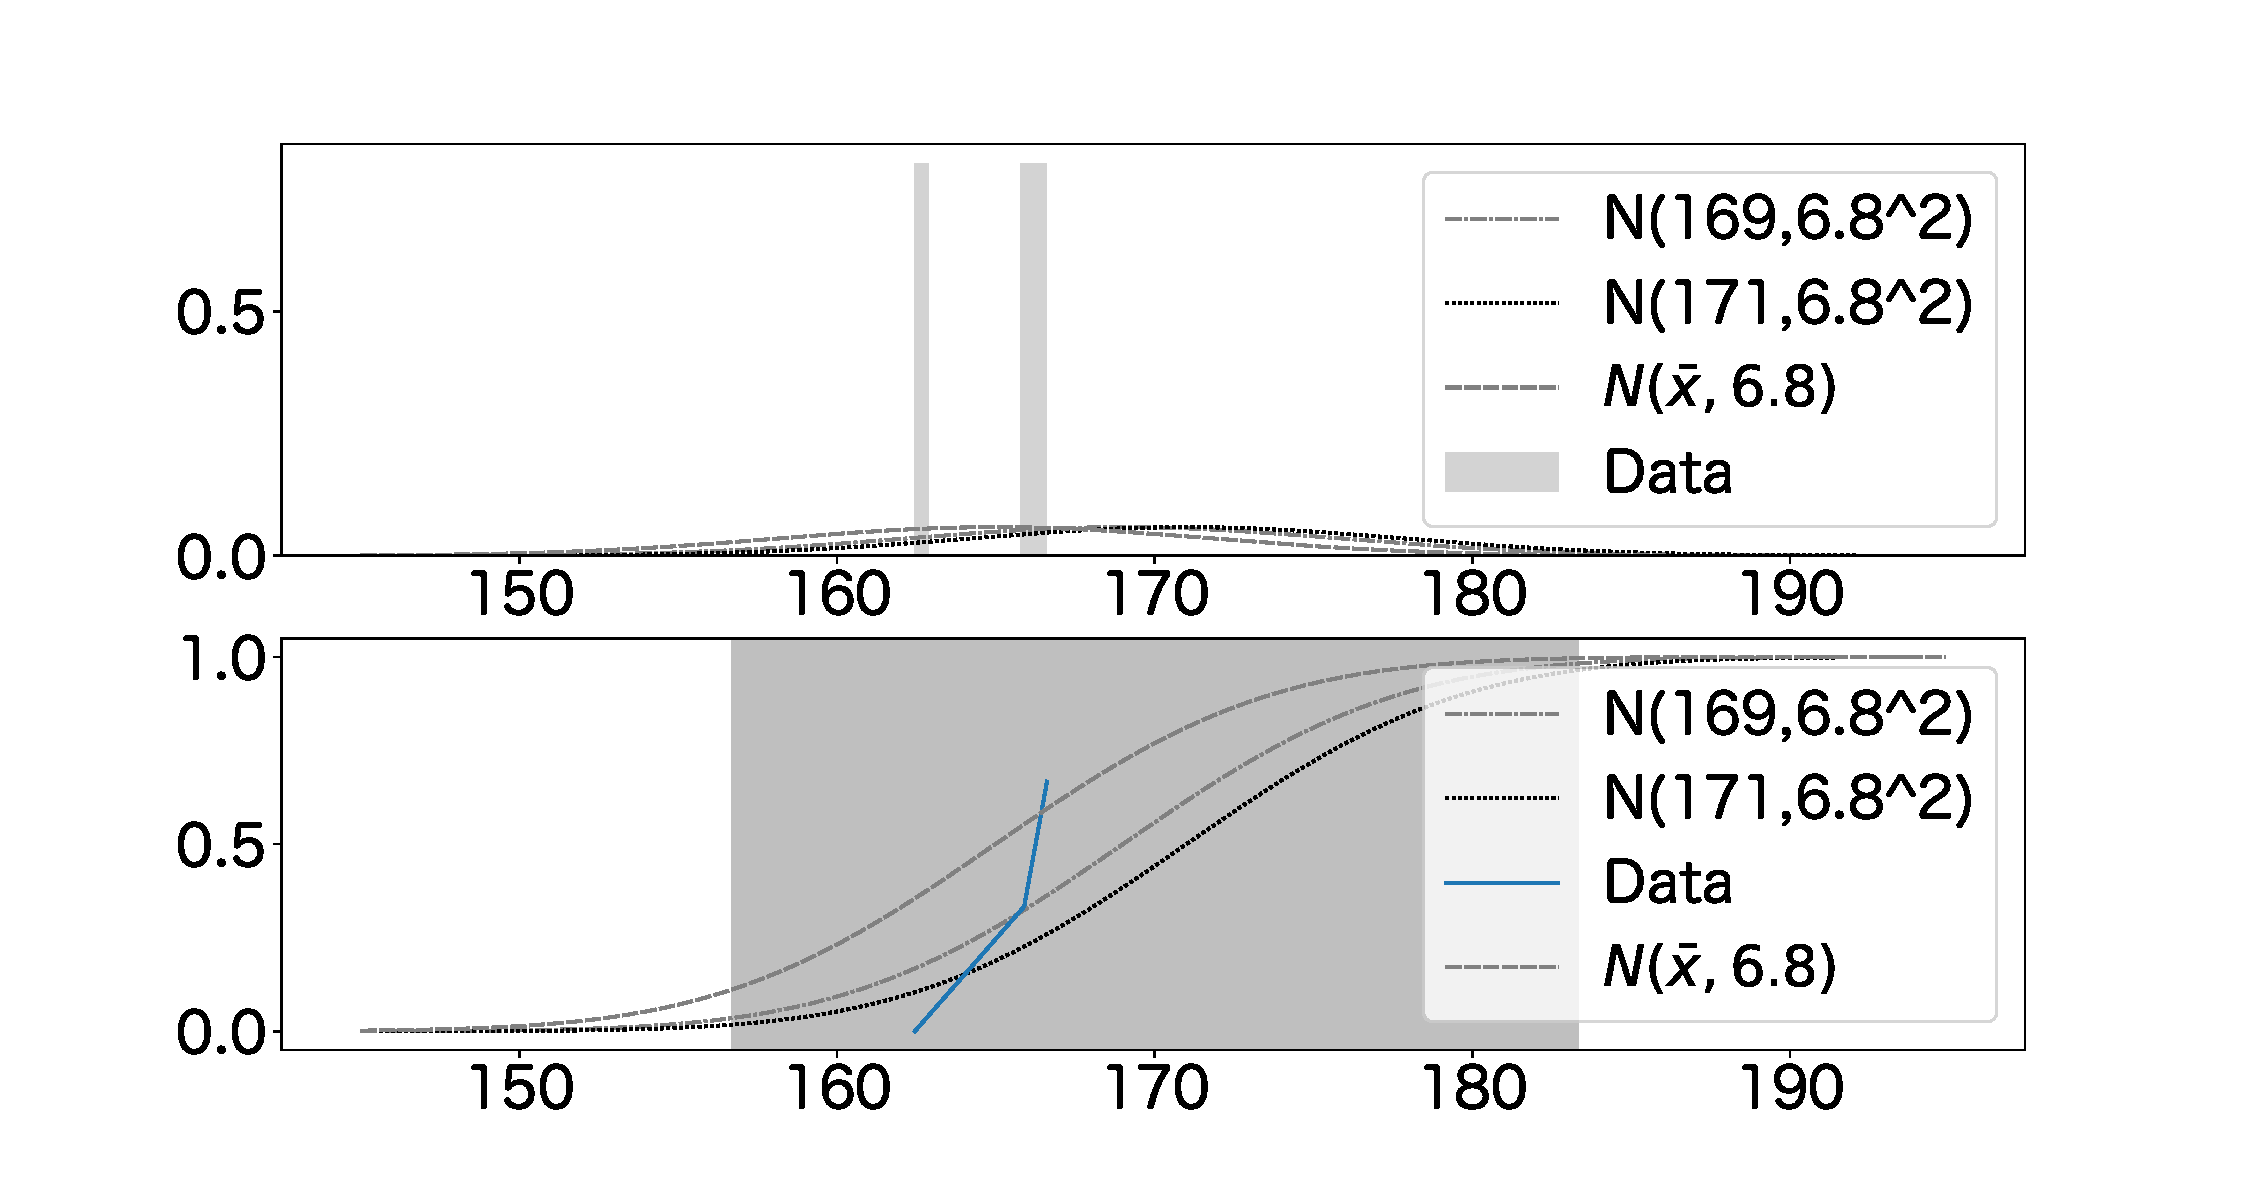
\includegraphics[width=15cm]{./image/02_/maximum_likelihood_3.pdf}
        \caption{$N(170,6.8^2)$からサンプルサイズ$3$の標本を得たときの分布。その最尤推定量により求められる分布関数。$N(168,6.8^2),N(171,6.8^2)$の分布関数を示す}
        \label{fig:maximum_likelihood_0}
    \end{center}
\end{figure}




\subsection{全然違うはなんとなくわかる}
図\ref{fig:maximum_likelihood_false_3},\ref{fig:maximum_likelihood_false_30}は、$N(170,6.8^2)$からサンプリングしたデータの度数分布と、その確率密度関数とは著しく異なる確率密度関数を表示したものです。

\begin{figure}
    \begin{center}
        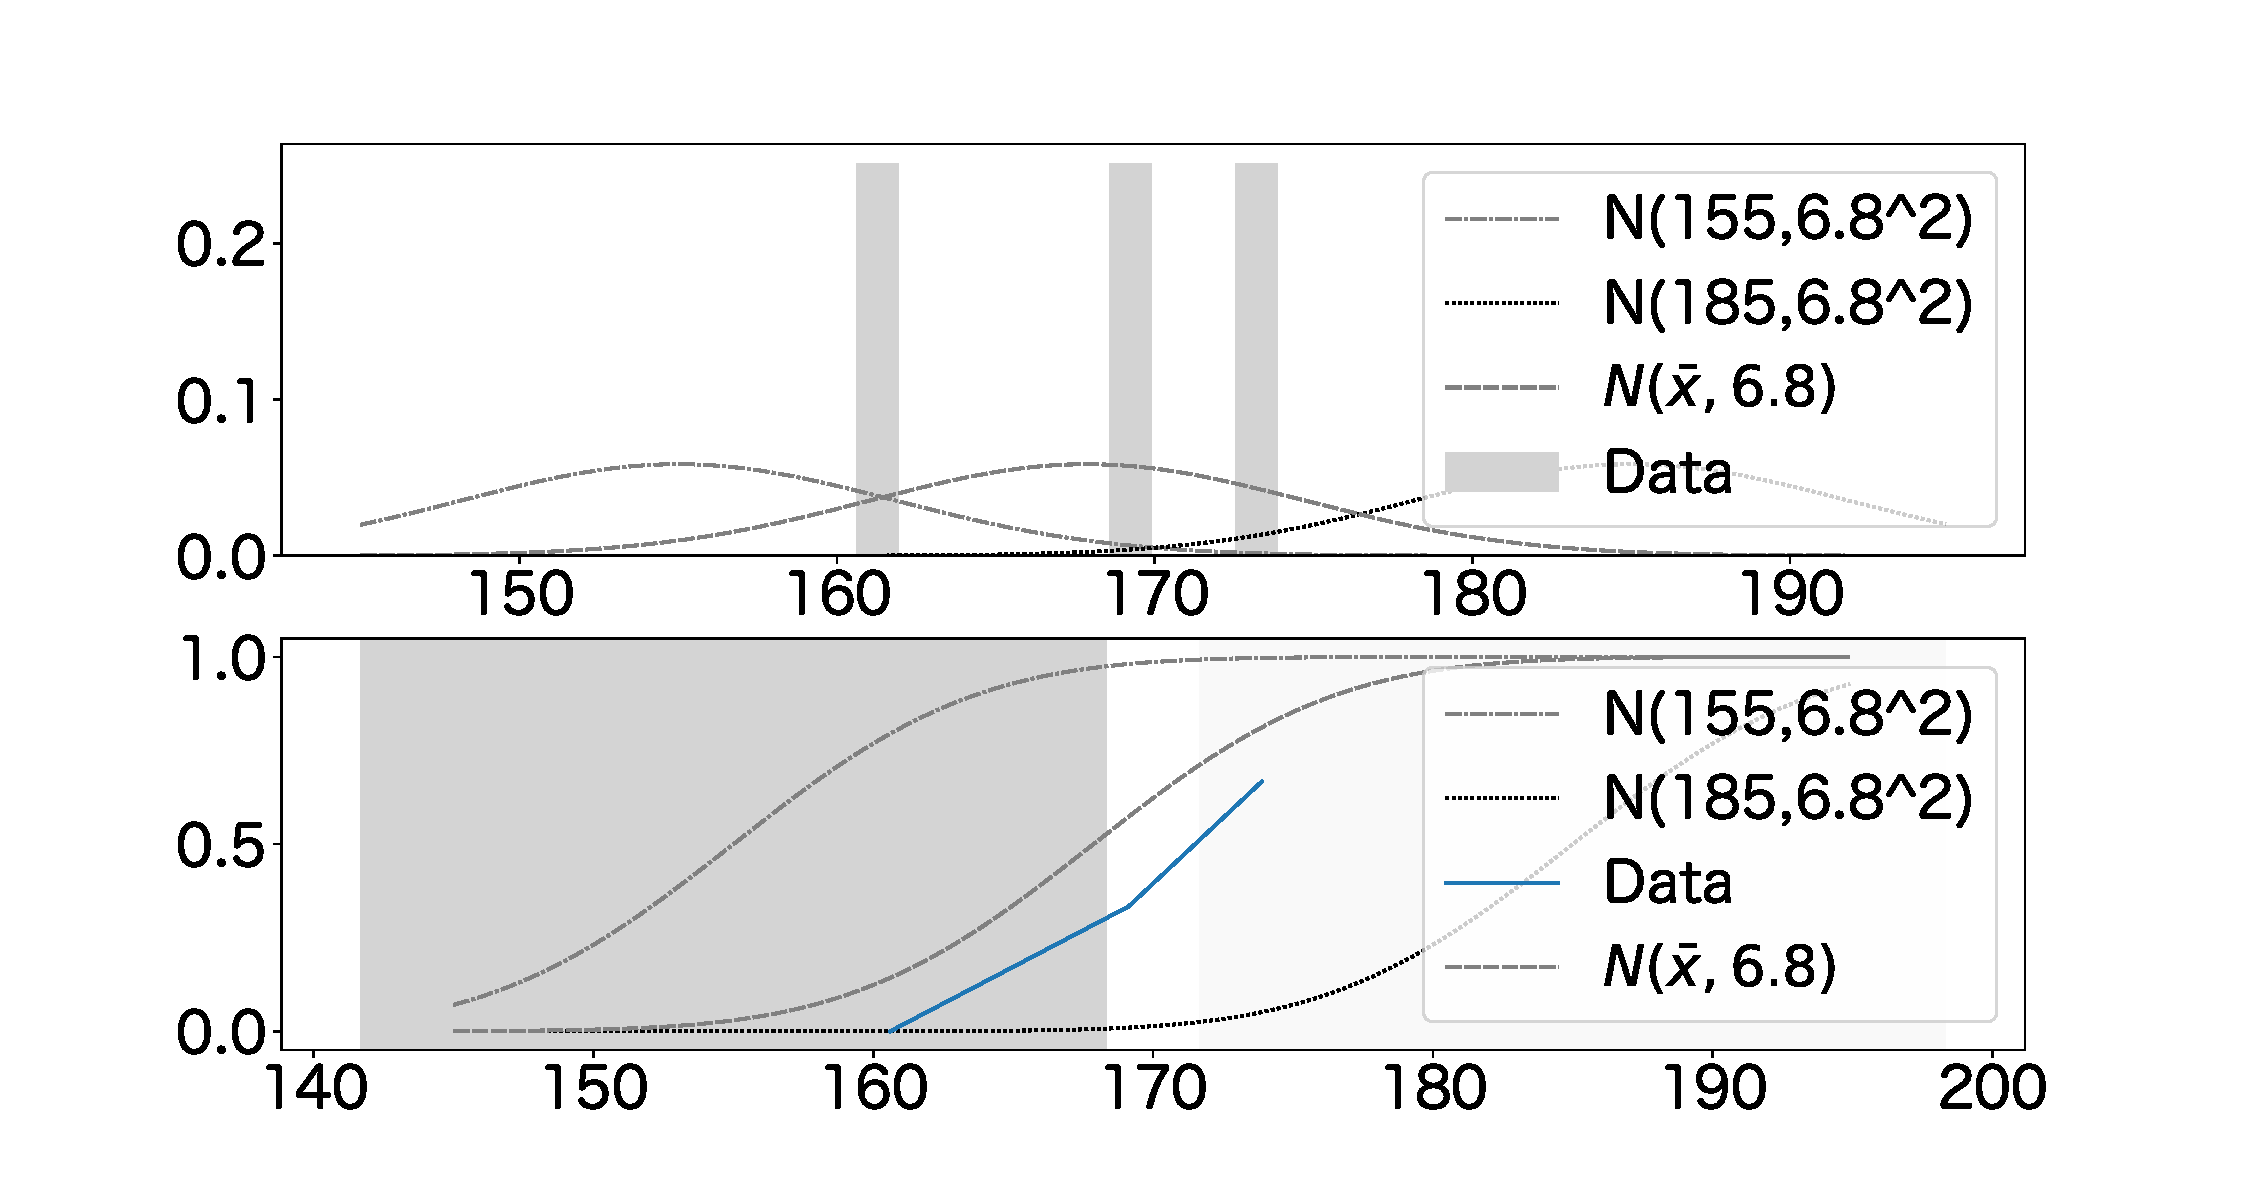
\includegraphics[width=15cm]{./image/02_/maximum_likelihood_false_3.pdf}
        \caption{$N(170,6.8^2)$からサンプルサイズ$3$の標本を得たときの分布。その最尤推定量により求められる分布関数。$N(168,6.8^2),N(171,6.8^2)$の分布関数を示す}
        \label{fig:maximum_likelihood_false_3}
    \end{center}
\end{figure}

\begin{figure}
    \begin{center}
        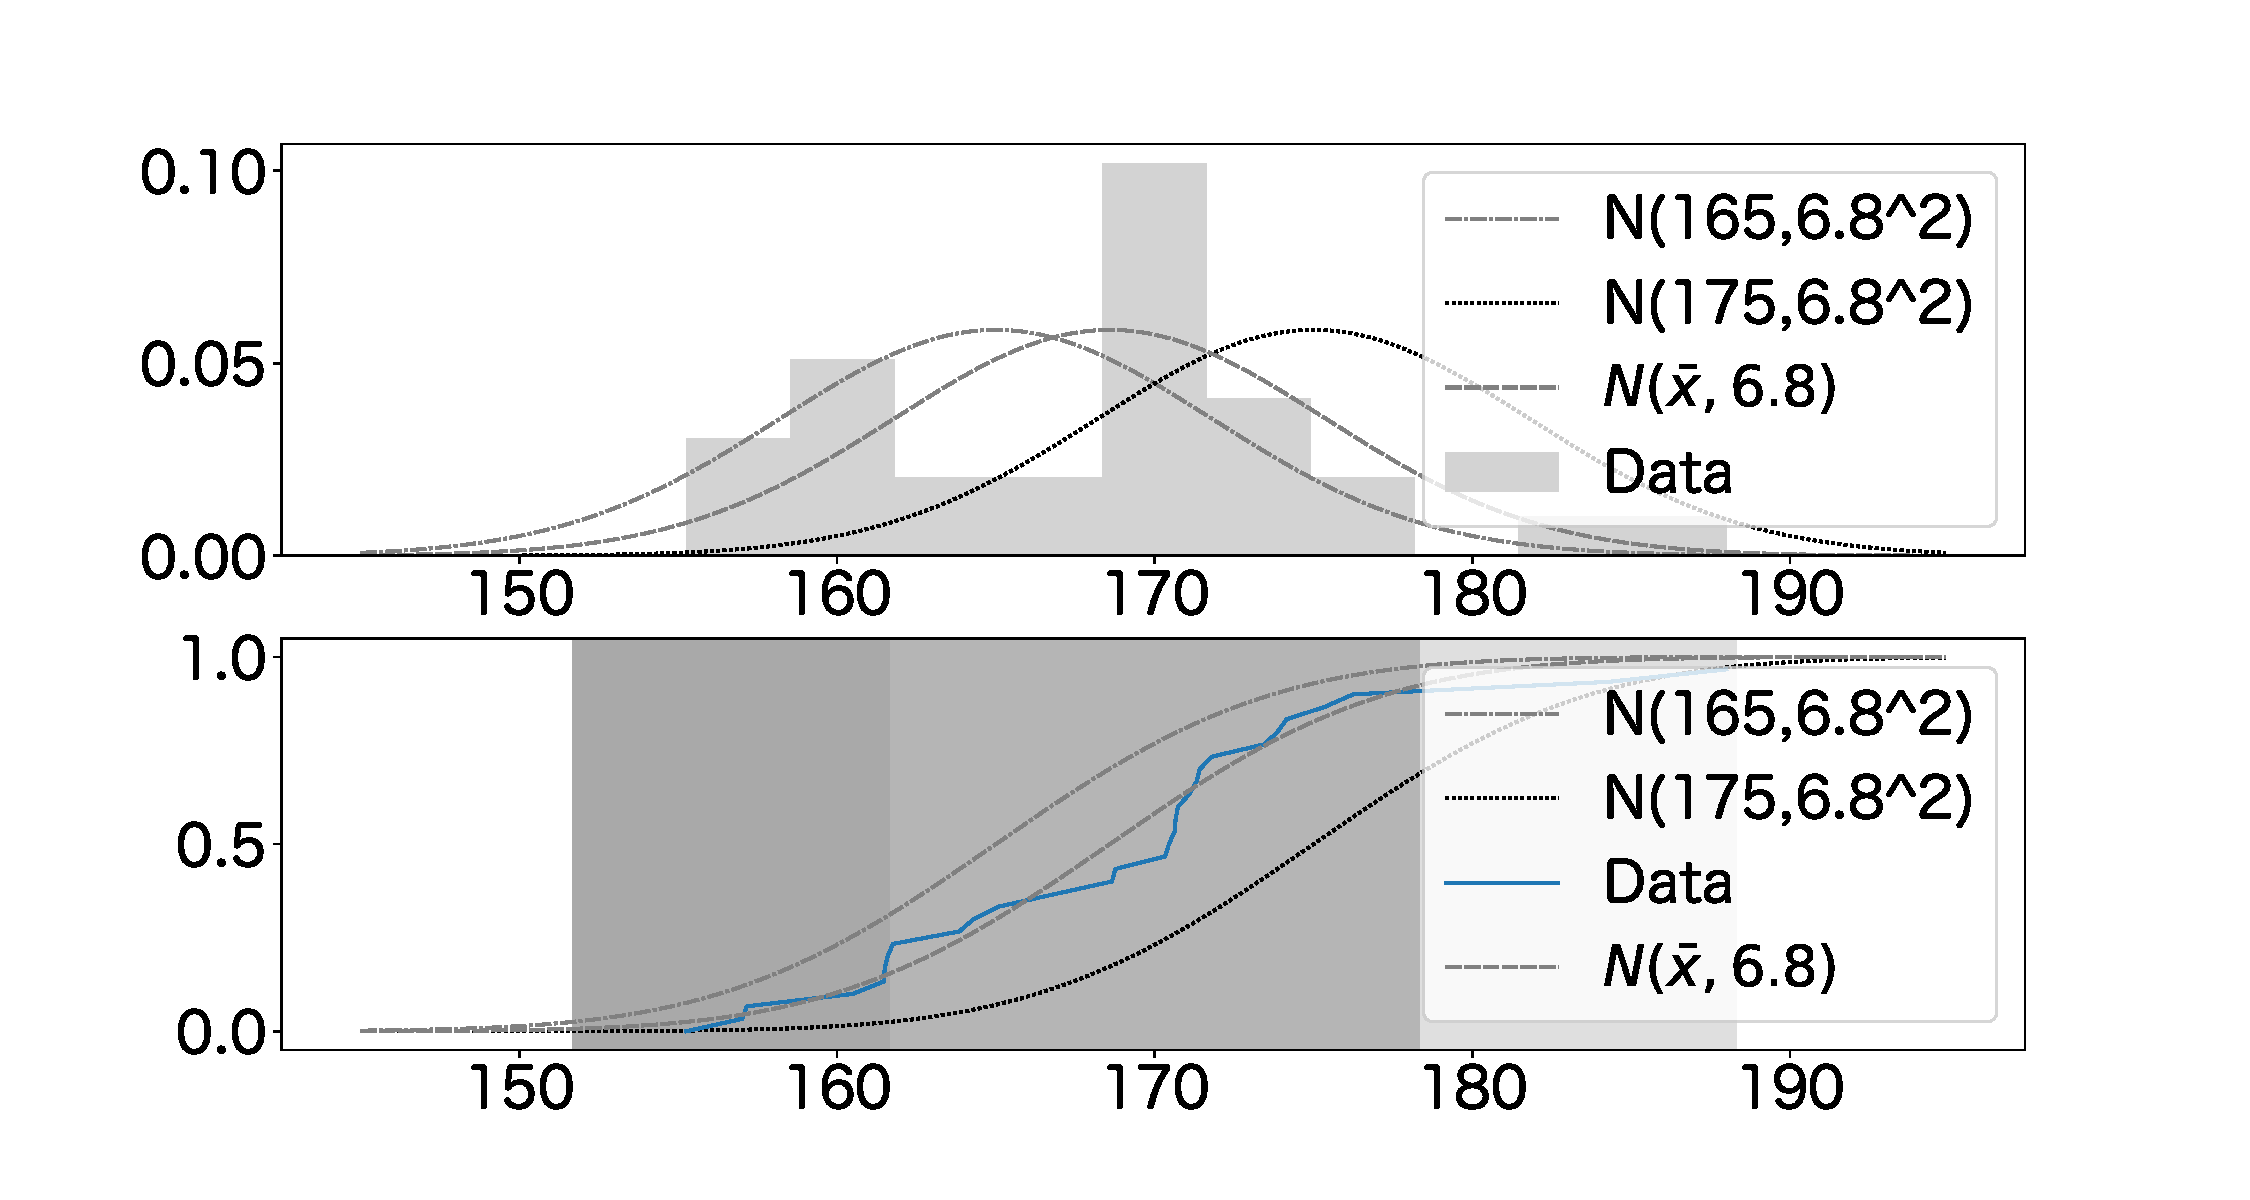
\includegraphics[width=15cm]{./image/02_/maximum_likelihood_false_30.pdf}
        \caption{$N(170,6.8^2)$からサンプルサイズ$3$の標本を得たときの分布。その最尤推定量により求められる分布関数。$N(168,6.8^2),N(171,6.8^2)$の分布関数を示す}
        \label{fig:maximum_likelihood_false_30}
    \end{center}
\end{figure}



\section{標本が統計モデルにより予測可能かを判定する}%統計モデルの性質を使った方法}
%ここまでは、統計モデルの予測がデータと一致することを定量的に評価した。
ここでは、推測に適していないと判断する方法である、統計的仮説検定を紹介する。
この方法は、統計量の一つである統計検定量の統計モデル上での出現しやすさにより、モデルを評価する。


\subsection{モデルの種類}

\begin{table}[hbtp]
    \caption{モデル}
    %\label{table:data_type}
    \centering
    \begin{tabular}{ccc}
      \hline
      モデルの仮定  & 棄却域  &  予測区間 \\
      $M(\mu_0,\sigma_0^2)$ $x_1,x_2,\cdots,x_n\sim N(\mu_0,\sigma_0^2)$  \\
      $\mu_0=\bar{x},\sigma_0^2=\frac{1}{n}\sum(x_i-\bar{x})^2$& -  &  - \\
      $\mu_0,\sigma_0$は設定値とする & $\frac{\sqrt{n}|\bar{x}-\mu_0|}{\sigma_0}\sim N(0,1)$  & $\mu_0-z_{\alpha/2}\frac{\sigma}{\sqrt{n}} <\bar{x}<\mu_0+z_{\alpha/2}\frac{\sigma}{\sqrt{n}}$ \\
      $\mu_0$は設定値,$\sigma^2$は未知 & 
      $|\frac{\bar{x}-\mu_0}{\frac{U}{\sqrt{n}}}| > t_{n-1,\frac{\alpha}{2}}$ただし、$U^2=\frac{1}{n-1}\sum(x_i-\bar{x})$
      %$\mu_0=\bar{x},\sigma_0^2=\frac{1}{n}\sum(x_i-\bar{x})^2$ 
      &  \\
      
      \hline
    \end{tabular}
  \end{table}


\subsection{問題意識}
確率変数$x_1$または、$x_1,x_2,\cdots,x_n$を得たとき、それらが独立同分布に従うという前提のもと、ある母数をもつ分布関数に従う、または従わないと推測することは可能であるだろうか。
最尤推定から、確率変数を得たなら、最尤推定を行って、母数を推測可能な場合がある。
具体的には、正規分布から得られた確率変数については、その平均と分散は、$(\mu,\sigma^2)=(\bar{x},\sum_{i=1}^{n} (x_i-\bar{x})^2/n)$である。

この問題に対して、
正規分布から確率変数を得たとき、ある母数平均$\mu$をもつ正規分布からサンプリングされていないということはできるだろうか。これを議論する。

%\subsection{問題点}
%aa

\chapter{科学的推論}
科学におけるモデルおよび、数理統計学におけるモデルについて説明し、その違いを明らかにする。


\section{モデル}
モデル(模型)とは、現実を表していると思わせるような、作られたものであり、次の特徴を備えています。
\begin{enumerate}
    \item モデルは本物の特徴の一部を推測可能。
    \item (1)を行うために、複数の仮定により構築される。また、それらの仮定は、現状の知識では明らかではないまたは、現実とは乖離していることがある。推測可能なことを増やすために仮定を増やすことがある。
    \item モデルは本物の要素・特徴の全体を推測することはできない。
    \item モデルは本物ではない。
\end{enumerate}
  
例えば、スケールを一定にした車のプラモデルはモデルの一つです。本物の特徴の一つである大きさを推測可能にするため、スケール(例えば、1/24など)を決めて作られている。車のプラモデルのドアや車体の幅を計測し、スケール倍すれば、本物の大きさを推測できる。本物の車がなくても、スケールを維持した車のプラモデルを持っていれば、簡単に推測が可能になる。
手のひらに収まるモデルを作ることができ、どこからでも観察することが可能である。

一方で、車のプラモデルがあったとしても、モデルの仮定によって推測可能なことが増えることがある。
例えば、本物のパーツの重量に応じて、モデルのパーツの重さを変化させる。
こうすることで、プラスティックでできたモデルの重さを計測すると、そこから本物の重さの推測が可能になる。
他にも推測したいこと、例えば、素材の質感や色や重量、または車の速度といった特徴なども、モデルに仮定を追加することで、本物の様子を捉えることが可能になっていく。


本物の車を持って来れば、本物の様子を推測することが可能であるので、車は、車自身のモデルということができる。
また、モデルの仮定を増やせば、本物の車にモデルを近づけることが可能である。
しかし、車を車自身のモデルとすると、それまであった利便性が損なわれる。
おおよその車体の長さが知りたいのに、わざわざ長い測りが必要になることや、手に持って観察することもできない。
このように、仮定を増やし細部まで推測可能にするというのは、デメリットになることがある。

本書では、モデルは本物ではないが、推測に役にたつ物として利用する。モデルと本物が極めて一致するように感じられることもあると思うが、モデルは本物ではない。

\section{統計モデル}


\subsubsection{分野によって異なるモデルの解釈}
モデルが本物であるか否かは、学問領域によって認識が異なっている。
生物物理学の視点では、モデルは現実を推測するための偽物のことだと考えていることの方が多い。
モデルが自分の知りたいことをうまく予測してくれさえいればいいという立場である。
一方で、数学では、モデルを現実と捉える傾向がある。モデルにより世界が支配されていると考えているのである。例えば、ある数学者は、流体モデルに解が安定的に存在するかがわからないから飛行機に乗りたくないと思っていると言う雰囲気がある。
現代の統計学はどちらかと言うと数学者が作った枠組みを統計ユーザーが受け入れてしまったため、ユーザーたちは、数学者のように世界を捉ようとしているように見える。


\begin{mybox}
    %\begin{quotation}
    \paragraph{頻度主義・ベイズ主義}
    頻度主義・ベイズ主義は統計学の流派を表す言葉である。頻度主義者であると言う人はあまり見たことがないが、ベイズ主義者はよく見る。ベイズ主義者は頻度主義者を非難するような主張をすることが多々ある。それぞれの立場を正確に説明した文献がないので、何を意味しているのかを私は理解できていない。

    おそらく、頻度主義では、モデルと母集団を一致させて考えており、このことを念頭にすれば頻度主義的な議論が理解できると思う。この立場にたてば、中心極限定理がデータにも適応可能になり、あらゆるデータが正規分布で推定可能にることを主張できる\footnote{本当にそう考えているのか確信が持てない}。
    %\end{quotation}
\end{mybox}


\subsection{統計モデル}
\begin{enumerate}
    \item モデルは現象の一部を表していると思わせるような、作られたもの
    \item モデルは不要な要素を削ぎ落とすために、大胆な仮定
    \item その仮定は、数理統計の知識を使う
    \item モデルは現象のことを推測できる
\end{enumerate}

モデルを作るとき、各仮定は、前提である必要はありません。実際と全く異なることを仮定しても良いですし、現象を扱うとなるとそうならざる得ないこともあります。

\begin{mybox}
    %\begin{quote}
        \paragraph{なぜ正規分布を仮定できるのか}
        %\begin{quote}
            学生のころ先生とデータについて議論していて(生物学分野です)「そもそもなぜ正規分布が仮定できるのか…」とおっしゃって二人でしばらく固まったことを思い出します。実現可能性の考え方から学ぶのが良いのかなと思います。
        %\end{quote}
        %\footnote{\url{https://twitter.com/katzkagaya/status/1209656621523058691}}
    %\end{quote}
\end{mybox}


\subsubsection{オッカムの剃刀}

仮定の追加には合理的な理由が必要だと考えられます\footnote{仮定を追加した統計モデルはベイズ統計と書かれた本で学ことができます。}。

\begin{figure}
    \begin{center}
%\includesvg{../markdown/section1/statistics_model.svg}
\end{center}
\end{figure}

\subsubsection{標本}


\subsubsection{サンプルサイズ、標本数}
\begin{defi}
母集団から無作為抽出して得た標本に含まれるデータの個数をサンプルサイズ(標本の大きさ)といい、その数を$T$や$n$で表す。同じ実験を繰り返して行ない、複数の標本を作ると、その標本の個数を標本数という。また、標本(サンプルサイズ)の大きさが大きい場合、大標本、小さいとき、小標本と言う。
\end{defi}
例えば、無作為抽出しデータを$20$個得る実験を30回繰り返した場合、サンプルサイズ$20$の標本を$30$得たことになります。言い換えれば、標本数$30$で、サンプルサイズは$20$であると言う。

サンプルサイズを標本数と言う流儀の統計学もあるようなので注意が必要である。
\footnote{ 業界によって様々な慣習があるので、業界の慣習に(師匠の言うことに)従った方がいいようにも思う\url{https://www.jil.go.jp/column/bn/colum005.html}。方言により定義が異なることがある文献がまとめられている\url{https://biolab.sakura.ne.jp/sample-size.html}。}


\chapter{取り扱うデータの条件}
科学的に事象を取り扱うための本書で扱うデータの条件は以下の通りである。
これらが無いならば、本書で扱える範囲を超えている。統計学者に相談した方が良い\footnote{最初から統計学者に相談した方が良い}。

\begin{itemize}
    \item 再現性 同じような条件であれば、同じような現象が生じるということである。
    \item 計測誤差  計測により生じた誤差(測定誤差)は揺らぎ(集団内での差)に比べて十分に小さい
    \item 無作為抽出 なるべく偏りなく母集団からデータを取得する%母集団の特徴を捉えるためのデータの収集方法
    \item 実験デザイン バイアスを小さくなるように計画を行う。
    \item 予測 データを集めると、データとモデルの予測に関して相違点が明らかになり、モデルの改訂が必要になる。この改訂に終わりはない。
\end{itemize}

%みたいものを見るための計測方法がランダムサンプリングである。
\section{実験デザイン}
わたしが扱える範囲ではないので、他書を読んだ方が良い。
今後まとめたい。

\section{無作為抽出されていない事による過誤}
対象を無作為に抽出できていない標本から、統計量を計算し、モデルの母数を推定したとする。
このモデルでは、本来設定した母集団に関する予測には誤りが多くなる。
例えば、17歳の日本人男性の身長を母集団に指定したのに、17歳のバスケ部部員の身長を計測する。
その標本を元に、モデルの母数を推定し、母集団に関する推測を行う。
すると、その予測は母集団に関して十分なものではなくなる。
例えば、平均が大きくなりすぎたり、平均よりも小さな人の割合が予測と異なることが生じる。
%その標本を元に、想定していた母集団に関しての推測を行おうとする。
%そうしたとき、その予測は母集団に関して十分なものではなくなる。

やってはいけないとは言い切れないが、偏った集団を計測してしまった場合、
その解釈に一工夫が必要になる。


\section{Questionable Research Practice(QRP)}
以下ではやってはいけないことを紹介する。
国立研究開発法人 日本医療研究開発機構が出版している研究公正に関するヒヤリ・ハット集の
「7 研究データの信頼性、再現性等 」に詳しくまとめられている\footnote{\url{https://www.amed.go.jp/content/000064531.pdf}}。

\subsection{後付けの母集団かつ$p<\alpha$を満たす集団}
母集団Aを設定し、標本を抽出したものを標本aとする。標本aのデータはさまざまな要素から構成されているとする。例えば、ある会社に所属する人の、身長や年収、税金の支払い履歴、ローン残高、労働部署、高校時代の部活などであるとする。
この標本から、何らかの属性$A'$に当てはまるデータbを抽出したとする。
データbについて特定の統計モデルとの乖離するかを調べ、乖離していることをが判明したとする(乖離を定量的に調べる方法はなんでもいいが、$p<\alpha$だったと考えても良い)。
この結果から、属性$A'$に関わると考えられる母集団A'を再構成する。
そこから、母集団$A'$を特定のモデルで予測できないと結論づけることはできない。

まず、今集めた標本$a$は、母集団$A$から集めたものであり、母集団$A'$から集めたものではない。
よって、母集団$A'$から無作為抽出できていない。
また、標本aを無作為抽出したときに付随して得た、母集団$A'$の一部の偏った集団のデータである。
以上から、母集団$A'$に関する無作為抽出とはいえない。
図\ref{fig:conceptual_diagram_HARKing}には、概念図を示しておいた。

\subsubsection{後付けの母集団かつ$p<\alpha$を満たす集団}
$p<\alpha$であるという標本がデータから発見されたので、標本の特性を持つと思われる母集団を後付けし、その母集団から無作為抽出を行なったことにし、ある統計モデルとデータが乖離していたと言うストーリーを作ったとする。
%統計モデルが棄却されたというストーリーを作ったとする。
言い換えれば、後付けの母集団ならば、$p<\alpha$であるという論理を立てたとする。
実際には、後付けの母集団でありかつ$p<\alpha$という集団から作為抽出しているので\footnote{この場合でも無作為抽出できていると誤解してしまうが、後付けの母集団から無作為抽出できていない!}、本来の母集団については何もわからない。言い換えれば、母集団に関する拡大解釈が行われたことで、母集団に関しては何もわからないのに、推測を行なったと主張している\footnote{実際調査した母集団は母集団かつ$p<0.05$に対して、報告した母集団デカすぎんだろ...}。
母集団の特徴を知るには、無作為抽出を行い、推測を行う必要がある。

\begin{figure}
    \begin{center}
        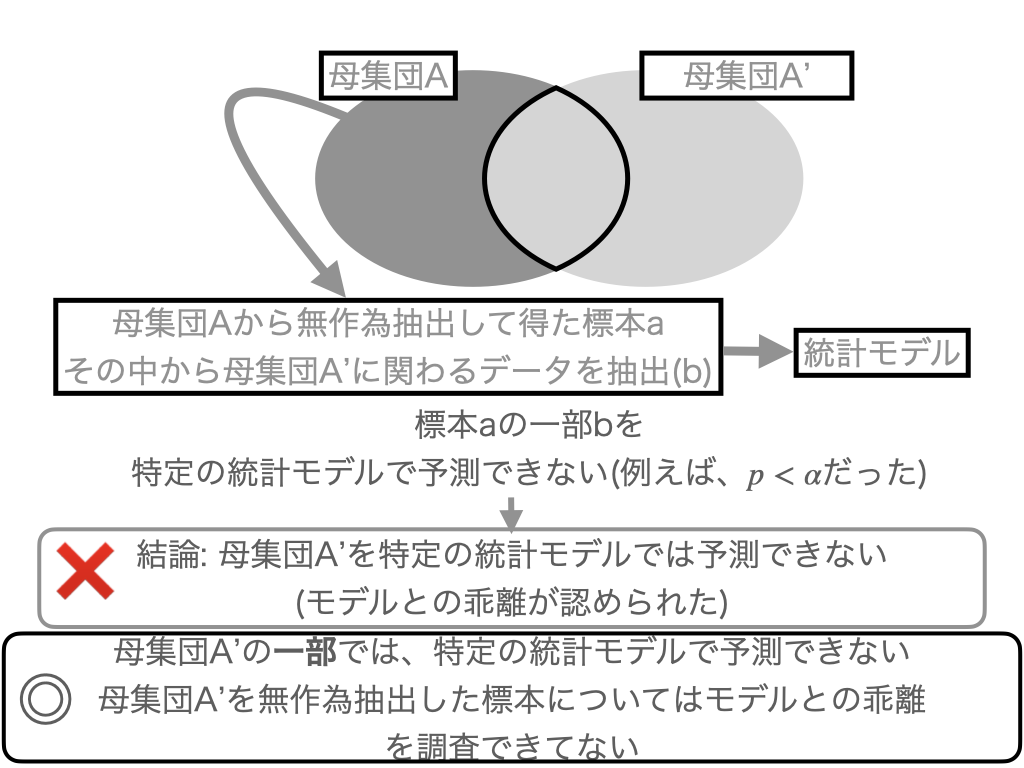
\includegraphics[width=15cm]{./image/01_/conceptual_diagram/conceptual_diagram.005.png}
        \caption{仮説ハッキングの概念図}
        \label{fig:conceptual_diagram_HARKing}
    \end{center}
\end{figure}
    

このような母集団に関する拡大解釈を仮説ハッキング($HARKing$(Hypothesizing After the Results are Known))といい、この操作により得たデータと仮説について、仮説が元からあったことにして、報告を行うと、研究不正となる\footnote{
    HARKingは、再現性の問題という意見もある。
    \url{https://twitter.com/ykamit/status/1077716200845500416} 。この意見に私は同意する。母集団を無作為抽出していないことで、再現できないことが増えると考えられる。
}
\footnote{
    多重検定により、$p$値が低く推測されることが問題であるというものもある\cite{池田_功毅2016,中村_大輝2021sp20016}。部分的には同意できるが、私は十分理解できなかった。
}\footnote{
    Twitterでのアンケートでは、多くの人がHARkingをうまく理解できてないというTwitterでのアンケートもある。
    \url{https://twitter.com/biomedcircus/status/1088957697368690689}
}\footnote{
    探索的なデータ解析においては、帰無仮説の後付けが許されるという主張もある。この意見には同意できない。母集団について拡大解釈をすることは許されない。探索的データ解析により得られるのは、母集団かつ$p<\alpha$という集団が見つかったということのみ主張できる。
    これを元に、母集団に関する性質を言及してしまうのはおかしい。
    %母集団についての推測をしたと主張はできない。
}\footnote{
    HARKingについては、\cite{kerr1998harking}に詳しくまとめられている
}。



\begin{SMbox}{HARKing}
    \begin{rightbubbles}{bubblegreen}{Yuki Kamitani}{./image/Twitter_logo_EPS/2021_Twitter_logo_blue.eps}
    データを操作してp値をいじる行為を不正と認識している人は多いが、HARKingが不正と思っている人は非常に少ない。私の周辺分野のシニア研究者で理解している人はほぼ皆無(問題を指摘すると一笑に付される)。研究の実践と論文フォーマットの齟齬やフェアプレー精神の問題(?)と理解している人がいた
        \begin{flushright} 
            \small	\url{https://twitter.com/ykamit/status/1077715969827528705}
        \end{flushright}    
    \end{rightbubbles}

    HARkingを理解するのは、難しい。無作為抽出したデータから、データを調べた後に、母集団を構成しているのだから、無作為抽出できていると考えてしまいがちになる。
\end{SMbox}
  

\subsection{$p<\alpha$になったら無作為抽出を終える}
$p$値がある値を下回ったときに、実験を終了するという操作を行なったとする。
統計モデルの予測と一致するように、母集団を選択したことになる。
この場合、無作為抽出した集団により、設定した母集団に関する性質を調べるという研究目的を達成できない。
「母集団かつ設定したモデルにおいて$p<\alpha$である」集団に関する調査を行なっていることになる。

調査を終えて、この標本についてモデルを使った予測ができないと主張できない。
この不正な操作をアステリスクシーキングという。


\subsection{標本平均がxxになったときに抽出を終える}
標本に対して計算できる平均値や分散が理想の(考えているモデル)と一致するまで無作為抽出を繰り返すまたは、一致したときに無作為抽出を終えると、無作為抽出したとは言いきれない。


\begin{SMbox}{計測したデータを報告しない}
    \begin{quote}
        日本製鉄は18日、東日本製鉄所君津地区(千葉県君津市)から有害物質が流出していた問題で、過去の水質測定データに不適切な扱いがあったと発表した。排出基準を超える有害物質が検出されたにもかかわらず、千葉県などに報告していない例があった。有害物質が基準を上回った際、再度測定して基準内に収まる結果を記録していたことも明らかにした。
        \ \ \\ \url{https://www.nikkei.com/article/DGXZQOUC186070Y2A810C2000000/}
    \end{quote}

    アンモニア化合物の漏洩が発生し、着色水の構外への流出が確認され、排水溝から取水したサンプルから、環境規制値を超えるシアンが検出される   \footnote{東日本製鉄所君津地区における着色水の構外への流出について \url{https://www.nipponsteel.com/common/secure/news/20220624_100.pdf}}。
    その後、シアン除去設備の能力増強などが行われる\footnote{\url{https://www.nipponsteel.com/common/secure/news/20220706_100.pdf}}。
    さらに、精査していくと、測定データについて不適切な取り扱いがあったことが判明した\footnote{\url{https://www.nipponsteel.com/common/secure/news/20220818_200.pdf}}。
    ここで、1日のうちに複数回の計測データが存在していたこと、関係機関へ報告していた数値より高い計測データが存在していたことが判明した。

    計測データが、予想や基準値よりも大きかったまたは小さかったから、データを削除してはいけない。
    計測手順を決定し、そして計測したデータは、全て報告しなければならない。

    データが恣意的に削除されているかどうかを判定することは非常に難しい。
    この例でも、データを持たない外部の人間が、不適切な報告が行われていることを判定できなかった。
    基準値を超えたデータについても記録が残っていたので、報告が適切に行われていないことが明らかになった。


    データがなければ、どのような行動を行うだろうか。
    例えば、保存されたサンプルを再度計測することになる。
    そのサンプルがなければ、なぜ基準値を超えた値が検出されたのかが徹底的にせいさされることになる。例えば、計測装置の利用手順のミスなどが検証される。
    ここで異常がなければ、通常のサンプリングが行われ、基準値を超えるデータが取得される頻度が、これまでよりも高いかを調べることになると考えられる。
    データがなければ、検証のコストが増えてしまうと考えられる。

    
    %川が赤くなっているという報告が上がったこともあり、調査が行われたようである\footnote{\url{https://news.yahoo.co.jp/articles/ea20d54623642b848960d93404aad6eba3ffae4a}}

\end{SMbox}

\chapter{統計モデル}
この章ではついにデータが登場する。データは母集団から無作為抽出によって得られた数値であるとする。
データを大文字の$X_1,X_2,\cdots,X_n$とし、モデルからサンプリングした確率変数を小文字の$x_1,x_2,\cdots,x_n$とする。
統計モデルはデータの出現頻度や統計量などを予測する。
まず、その予測可能なことについて列挙する。モデルとデータが異なる場合つまり、データの出現頻度をデータが予測できない場合に生じることについて説明する。

\section{正規分布を含んだ統計モデル}
次の3つを仮定したモデルを正規モデルと呼ぶ。
\begin{quote}
    \begin{enumerate}[(1)]
    \item 独立同分布
    \item その分布は、正規分布
    \item 正規分布の母数(平均と分散)はそれぞれ$\mu,\sigma^2$。
    \end{enumerate}
\end{quote}
この正規モデルを$M(\mu,\sigma^2)$と書く。$\sigma^2$をある特定の値にしたときのモデルを$M(\mu)$とし、$\mu$を特定の値にしたモデルを$M(\sigma^2)$とする。

%\subsection{最尤推定量を使ったモデル}
母集団から無作為抽出した標本を元にモデルを構築する。具体的には、$\mu_{ML}=\bar{X},\sigma^2_{ML}=\frac{1}{n}\sum(X_i-\bar{X})$とし、統計モデル$M(\mu_{ML},\sigma^2_{ML})$を最尤モデルと呼ぶ。

以下では、$M(\mu)$による予測について説明する。

\if 0 
このモデルにおいて、統計量$Z(\bar{x},\mu)$の$95\%$予測区間を求める。
%よく入る区間の式を変形し、データを得たときに、そのデータを基準にした$\mu$の範囲に変形してみます。
\begin{eqnarray*}
 & -z_{0.025} < Z(\bar{x},\mu)<z_{0.025} \\
\rightarrow & -z_{0.025} < \frac{\sqrt{n}(\bar{x}-\mu)}{\sigma}  <z_{0.025} \\
\rightarrow & \bar{x}- z_{0.025}\frac{\sigma}{\sqrt{n}} < \mu < \bar{x} + z_{0.025}\frac{\sigma}{\sqrt{n}}
\end{eqnarray*}
\fi

\if 0

\section{問題意識}
確率変数$x_1$または、$x_1,x_2,\cdots,x_n$を得たとき、それらが独立同分布に従うという前提のもと、ある母数をもつ分布関数に従う、または従わないと推測することは可能であるだろうか。
最尤推定から、確率変数を得たなら、最尤推定を行って、母数を推測可能な場合がある。
具体的には、正規分布から得られた確率変数については、その平均と分散は、$(\mu,\sigma^2)=(\bar{x},\sum_{i=1}^{n} (x_i-\bar{x})^2/n)$である。

この問題に対して、
正規分布から確率変数を得たとき、ある母数平均$\mu$をもつ正規分布からサンプリングされていないということはできるだろうか。これを議論する。

%\subsection{問題点}
%aa
\fi

\subsection{データが出現しやすい区間}
ある決められた確率でデータが出現するとモデルが予測する区間を予測区間という。
割合として、よく使われる$95\%$を設定したものを$95\%$予測区間という。
正規分布を含んだモデル$M(\mu)$において、予測区間は比較的簡単に求めることができる。
具体的には、正規分布の規格化を行い、標準正規分布に従うように変換を行い、$\frac{x-\mu}{\sigma}$であるので、予測区間は、
\begin{eqnarray*}
    %-z_{0.05} <\frac{x-\mu}{\sigma} <z_{0.05} \\
    \mu-z_{0.05}\sigma < x < \mu+z_{0.05}\sigma
\end{eqnarray*}
である。この範囲に$95\%$のデータが生じることをモデルが予測する。実際にそのようになるかは不明であり、予測であることを意識した方が良い。

$68\%$の確率でデータを含むと予測する区間が求められる。
\begin{eqnarray*}
    %-z_{0.05} <\frac{x-\mu}{\sigma} <z_{0.05} \\
    \mu-\sigma < x < \mu+\sigma
\end{eqnarray*}

\subsubsection{母集団の標本が指数分布的に分布していた場合}
母集団の分布形と統計モデルに含まれている確率分布関数が著しく異なる場合を考える。
母集団分布として、指数分布を仮定しする。これは、自然から指数分布的なデータが得られたときのことを想定している。
これを予測するモデルを正規分布の仮定されたモデルとする。
\if 0
を使い、最尤モデルにおける平均値は、
$\bar{x}\sim N(\mu_{ML},\sigma^2_{ML}/\sqrt{n})$である。
このことから、モデルは、$\left[ \mu_{ML}-z_{0.05}\sigma_{ML},\mu_{ML}+z_{0.05}\sigma_{ML} \right]$
の間に、$68\%$の確率で平均値が入ることを予測する。
\fi
最尤モデルは、$M(\mu_{ML},\sigma^2_{ML})$である。ここから、
\begin{eqnarray*}
    %-z_{0.05} <\frac{x-\mu}{\sigma} <z_{0.05} \\
    \mu_{ML}-\sigma_{ML} < x < \mu_{ML}+\sigma_{ML}
\end{eqnarray*}
が$68\%$予測区間になる。
言い換えれば、標準偏差の間に、サンプルの平均が入る確率が$68\%$であることをモデルが予測している。
このことを数値シミュレーションにより確かめる。
指数分布からランダムサンプリングを行い、無作為抽出によりサンプルサイズ$10^6$の標本を得たとする。
サンプルが上記の区間に入っている割合を計算する。

\begin{lstlisting}
N = 10**6
sample = expon.rvs(scale=10,size=N)
#sample = norm.rvs(loc=0,scale=1,size=N)
lambd= np.average(sample)
print(np.average(sample),np.std(sample),np.var(sample))

mu = np.average(sample)
s = np.std(sample)

a,b = mu-s,mu+s
len(sample[np.where( (sample >a) & (sample<b) )])/N
\end{lstlisting}
この結果、期待していた値$68\%$よりも著しく大きな確率$86\%$程度を得る。
これは、モデルでは、正規分布を仮定していたが、実際には指数分布的なデータだったために生じる予測の間違いである。
以上でわかるのは、統計モデルと実際の母集団が乖離している場合には、標準誤差に間違いが多くなるということである。

\subsubsection{エラーバー(SD)から読み取れること}
正規分布と指数分布それぞれからサンプルサイズ$N=100$の標本を作り、プロットした(図\ref{fig:sample_norm_expon_model})。それぞれの分布の右側のエラーバーは、$68\%$予測区間。
標本が正規分布であるときには、$68\%$予測区間の中におよそ$68\%$のデータが含まれている。
一方で、標本が指数分布であるときは、モデルの予測と乖離する。このことは、図から読み解くことが難しい。

エラーバー(SD)だけが描かれた図を見るとデータに対する印象が変わる(図\ref{fig:model_predict_SD})。
図\ref{fig:model_predict_SD}には、正規分布と指数分布から得られた標本から、最尤推定を行ったモデル$M(\mu_{ML},\sigma^2_{ML})$における$68\%$予測区間を描画している。
データが正規分布的であるならば、データが区間に入っている割合が予測と一致する。
一方で、データが指数分布的であるならば、モデルの予測(エラーバー)から得られることと、実際のデータは乖離する。
エラーバーからは、中央からデータが対称に分布しており、その中に、$68\%$のデータが入っていることを読み取れる。
実際のデータは図\ref{fig:sample_norm_expon_model}にある通りであり、モデルの予想とは一致しない。

エラーバーにSDを描くときには、特に指定がない限り、正規分布を仮定したモデルを想定しているということが予想される。
実際には、モデルを考えてエラーバーを書いていると断言しがたい。
SDが描かれているのに、検定においては正規分布を仮定しない統計モデルを使っていることも多々ある。
データの描画においては、正規分布を仮定しているにもかかわらず、統計においてはその仮定による推測をやめている。
この場合、著者が何を考えてSDを描いたのか判別しにくい。
%また、データが正規分布的であることに確信を得ることは、サンプルサイズを大きくした標本から想像するしかなく、費用がかさむので行われない。
%このこと、モデルの予測が当たることを肯定できる根拠がないことを意味する。

測定の精度の良さを示す指標としてSDを書くことがある。この場合、ただ単にSDが小さければ良い。
%データが正規分布であるという強い前提がある。

\begin{figure}
    \begin{center}
        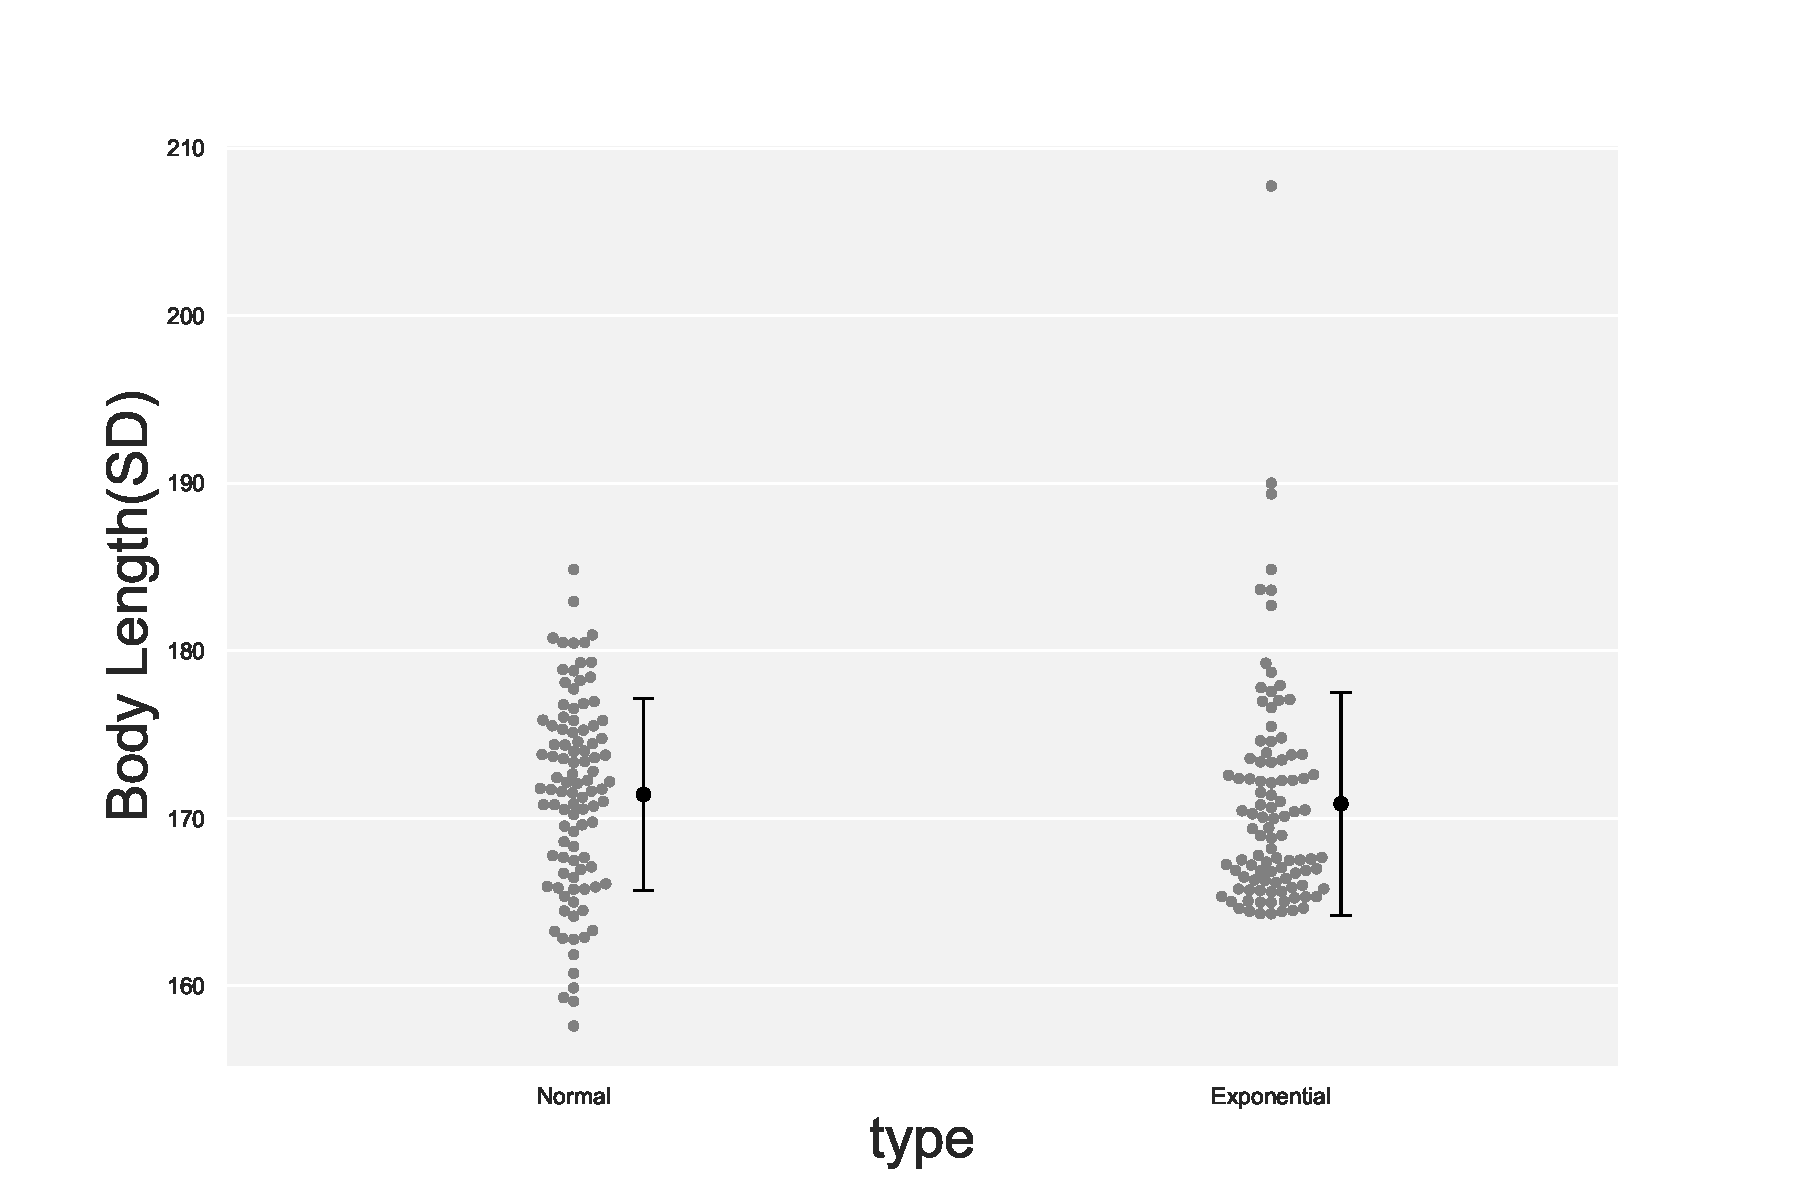
\includegraphics[width=15cm]{./image/12_/sample_norm_expon.pdf}
        \label{fig:sample_norm_expon_model}
        \caption{正規分布と指数分布それぞれからサンプルサイズ$N=100$の標本をプロットした。それぞれの右側にあるエラーバーは、正規分布モデルが予測した$68\%$予測区間。}
      \end{center}
    \end{figure}


\begin{figure}
    \begin{center}
        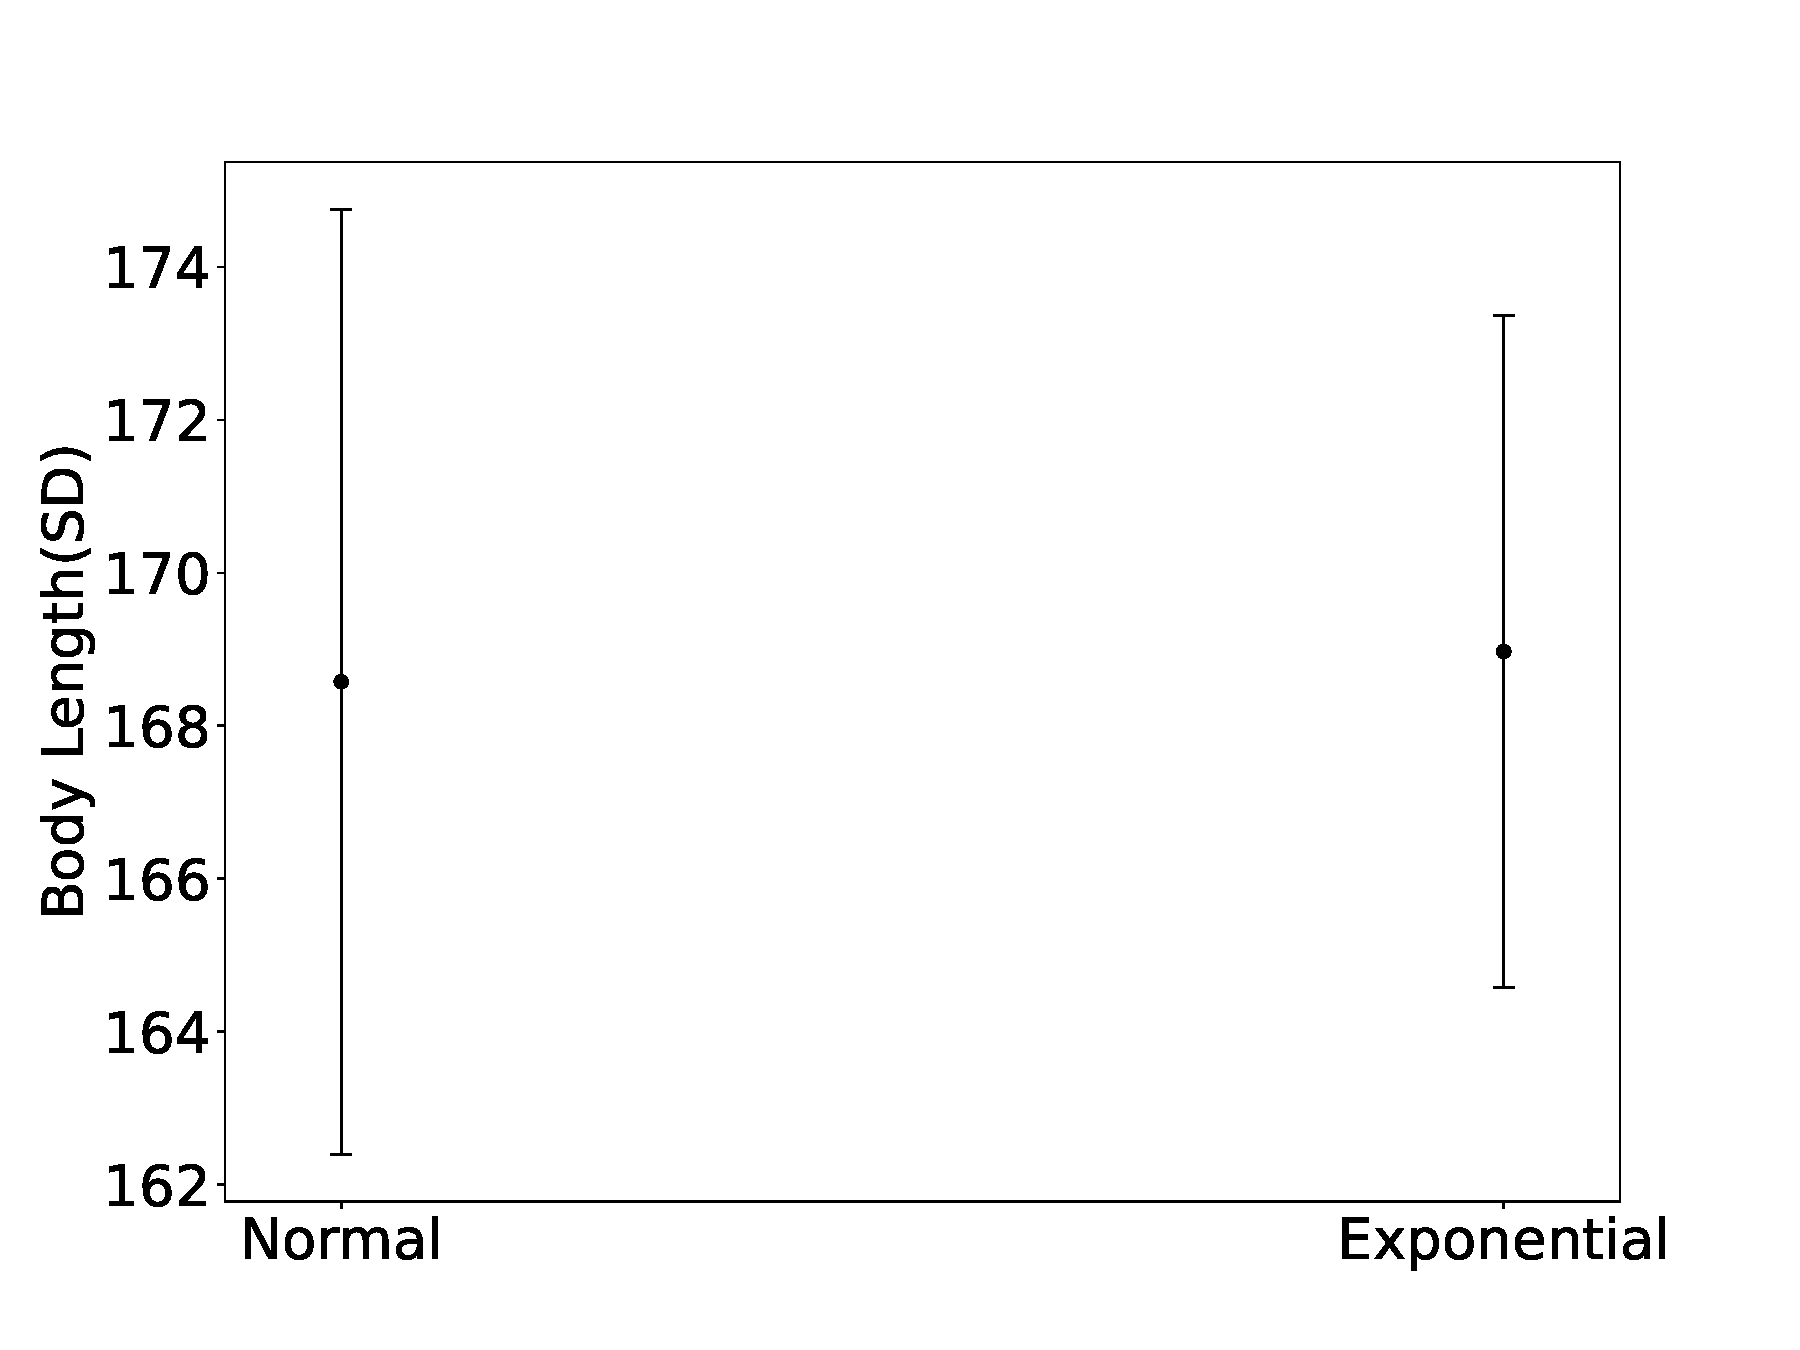
\includegraphics[width=15cm]{./image/12_/model_predict_SD.pdf}
        \label{fig:model_predict_SD}
        \caption{正規分布と指数分布それぞれからサンプルサイズ$N=100$の標本を得た。その標本から推測される$68\%$予測区間を描画した。}
      \end{center}
    \end{figure}


\subsection{平均値が出現する区間}
今回考えている統計モデル$M(\mu)$では、次の統計量$Z$が標準正規分布$N(0,1)$に従うことが、正規分布の再生性によってわかっている。
$$
Z(\bar{x},\mu)=\frac{\sqrt{n}(\bar{x}-\mu)}{\sigma} \sim N(0,1)
$$
ここで$\bar{x}$は、統計モデル$M(\mu)$からサンプリングした標本の標本平均値(データの平均値ではない)、$\mu,\sigma$は統計モデルで設定した母数平均、母数分散。
%$Z(\bar{x},\mu)$が$N(0,1)$に従うということから、$Z(\bar{X},\mu)$が$N(0,1)$における出現頻度が計算できる。
\begin{figure}
    \begin{center}
        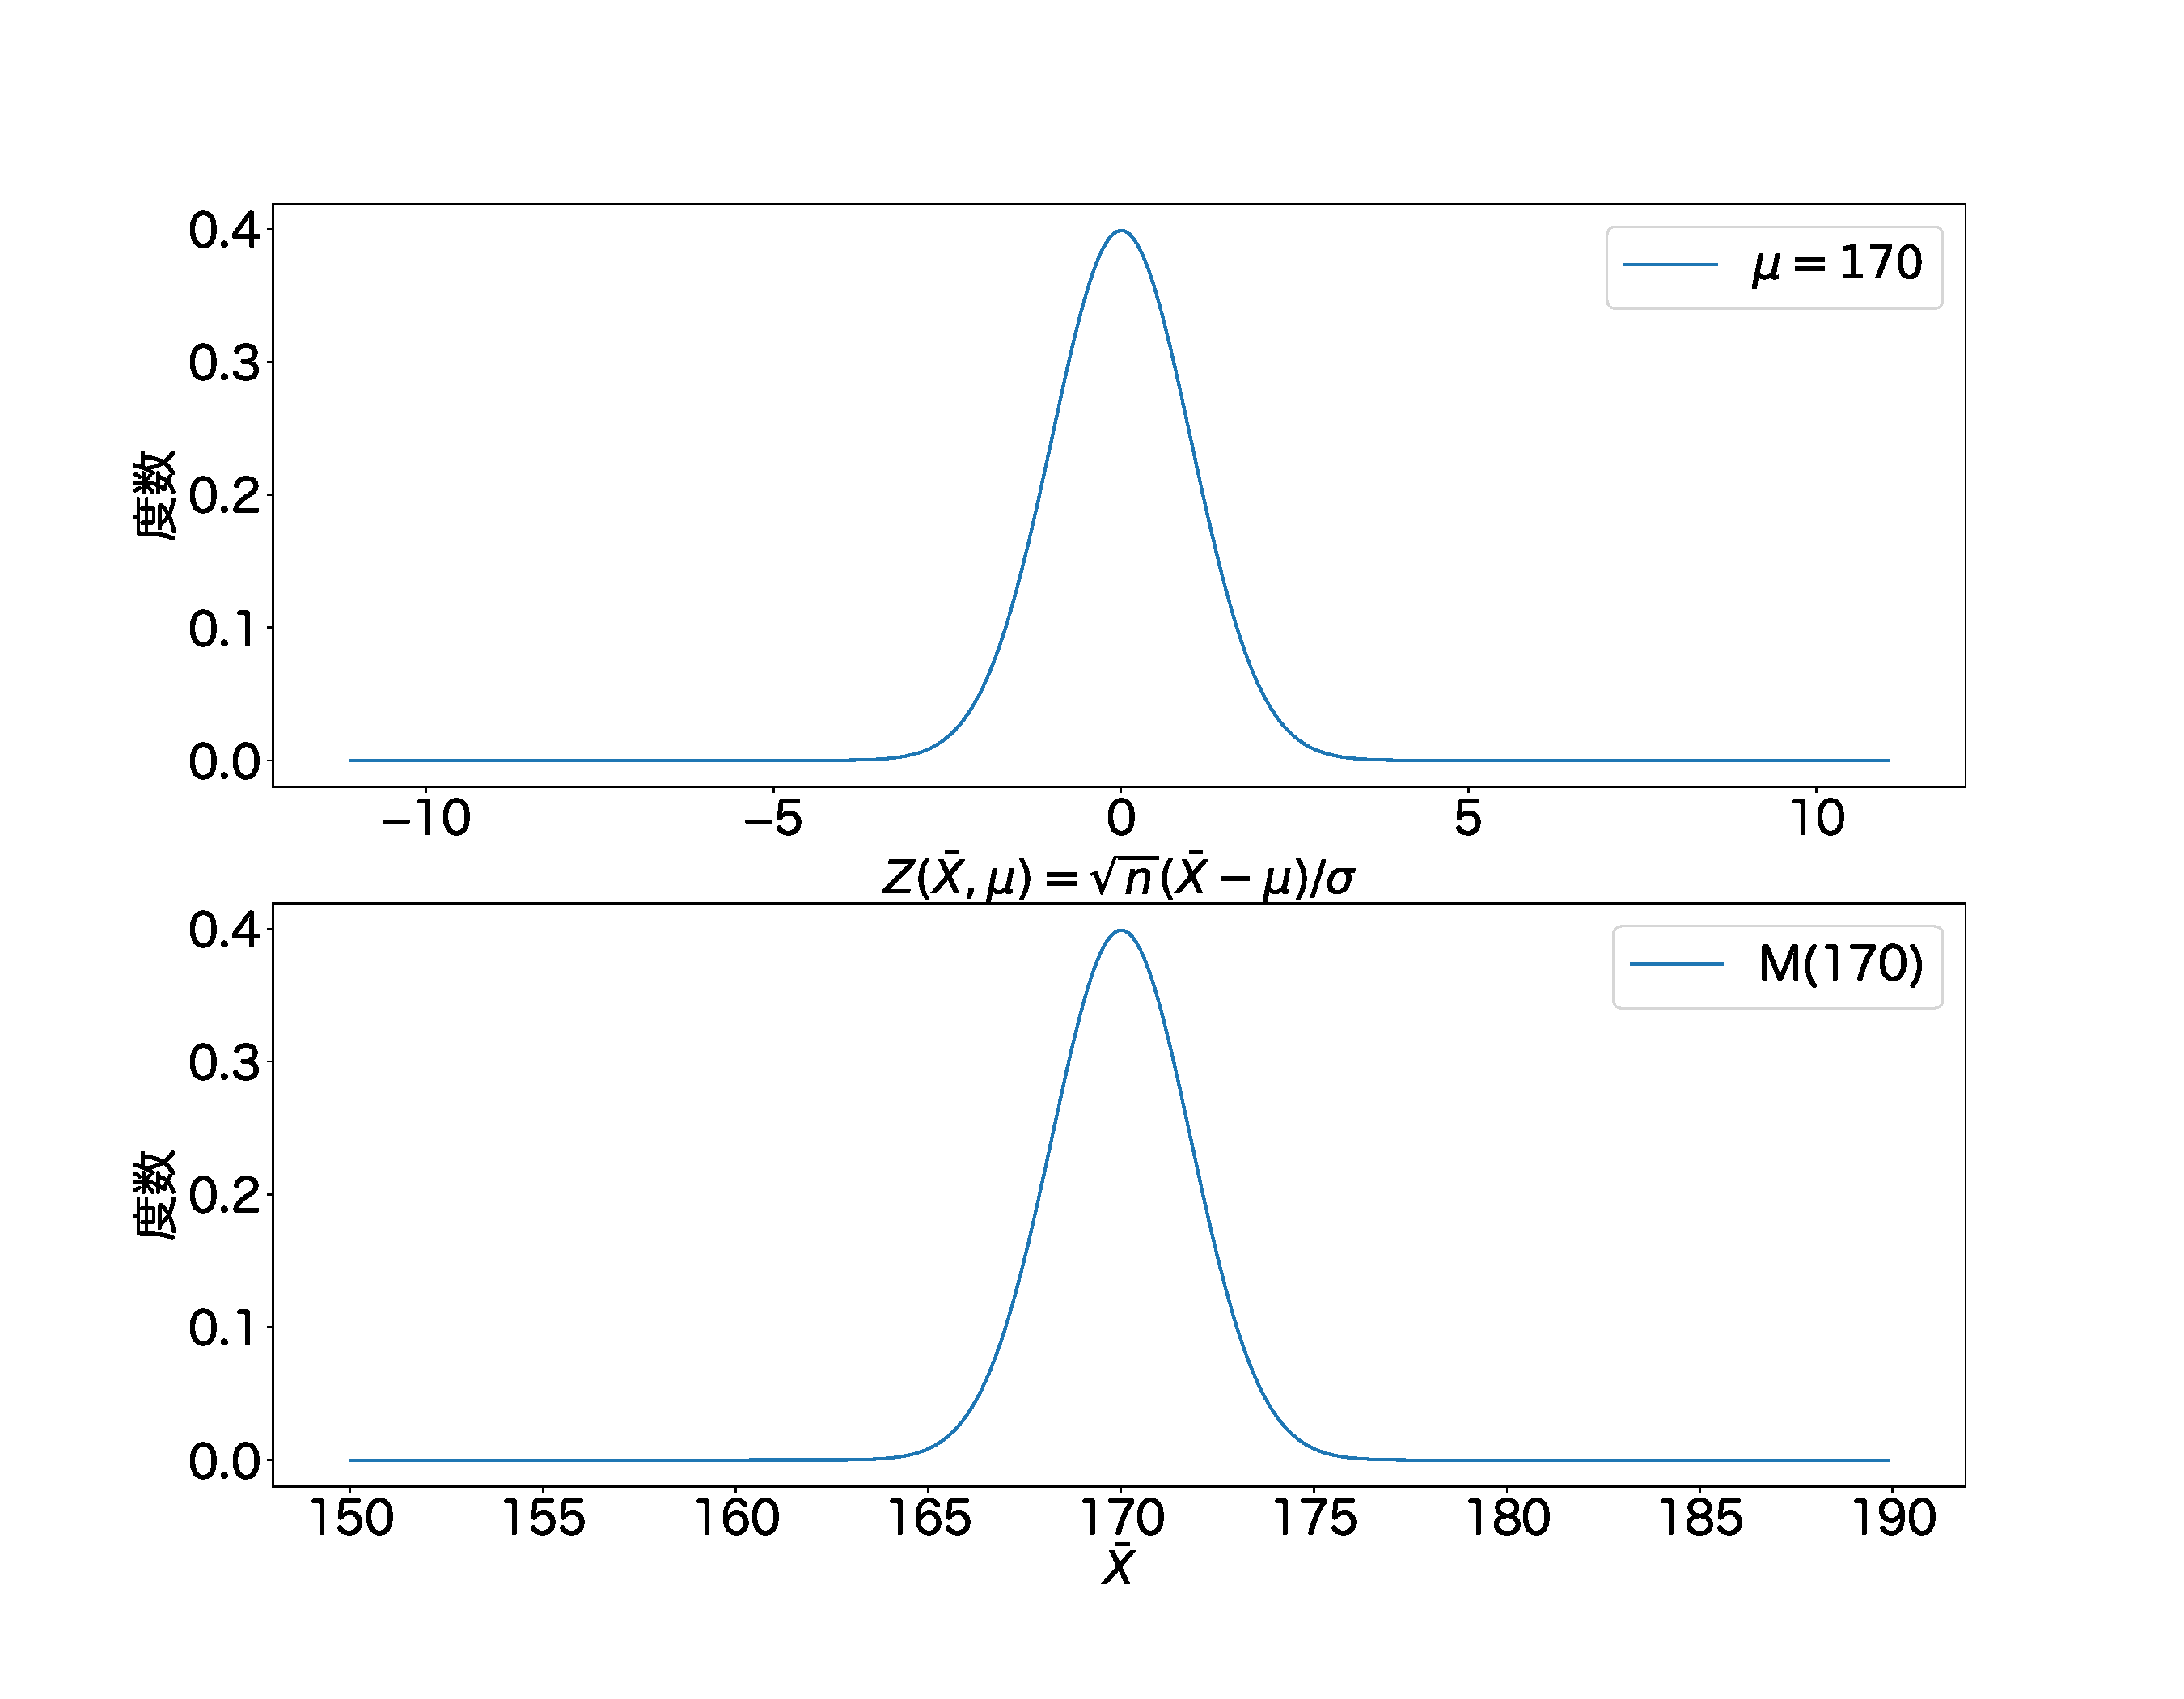
\includegraphics[width=15cm]{./image/03_/normal_Z_frequency.pdf}
        \label{fig:cm_standard_normal_distribution}
      \end{center}
    \end{figure}

$Z$の出現頻度を$Z$または$\bar{x}$の値に応じて書いたものが図\ref{fig:cm_standard_normal_distribution}である。
$Z(\bar{x},\mu)$の$95\%$予測区間が次のように求められる。
$$
-z_{0.025}<Z(\bar{x},\mu)<z_{0.025}
$$
これは、サンプリングされた標本の統計量$Z(\bar{X},\mu)$が$95\%$の確率で得られる範囲である。
統計モデルを使った判断でよく出てくる確率として分野を問わず、$95\%$が使われる。
%この値には身長に関する経験を使わずに決定しています。


$Z(\bar{X},\mu)$を式変形することで、標本平均が$95\%$の確率で出現する区間が推定できる。式を変形する。
\begin{eqnarray*}
    & -z_{0.025} < Z(\bar{X},\mu)<z_{0.025} \\
\rightarrow & -z_{0.025} < \frac{\sqrt{n}(\bar{X}-\mu)}{\sigma}  <z_{0.025} \\
\rightarrow & \mu - z_{0.025} \frac{\sigma}{\sqrt{n}} < \bar{X} < \mu + z_{0.025} \frac{\sigma}{\sqrt{n}}
\end{eqnarray*}
この統計モデルからサンプリングした標本の標本平均$\bar{x}$が$95\%$の確率で見つかる範囲のことを$95\%$信頼区間という。これも、モデルの予測である。

\subsubsection{サンプルサイズによる影響}
$95\%$信頼区間を見てわかるように、サンプルサイズ$n$が大きくなれば、$\bar{x}$が入る範囲は狭くなる。
信頼区間がサンプルサイズに依存することを数値的に確認する。
図\ref{fig:confidence_interval_n}は、信頼区間が$N$に応じて変化する様子を図示した。

\begin{figure}
\begin{center}
    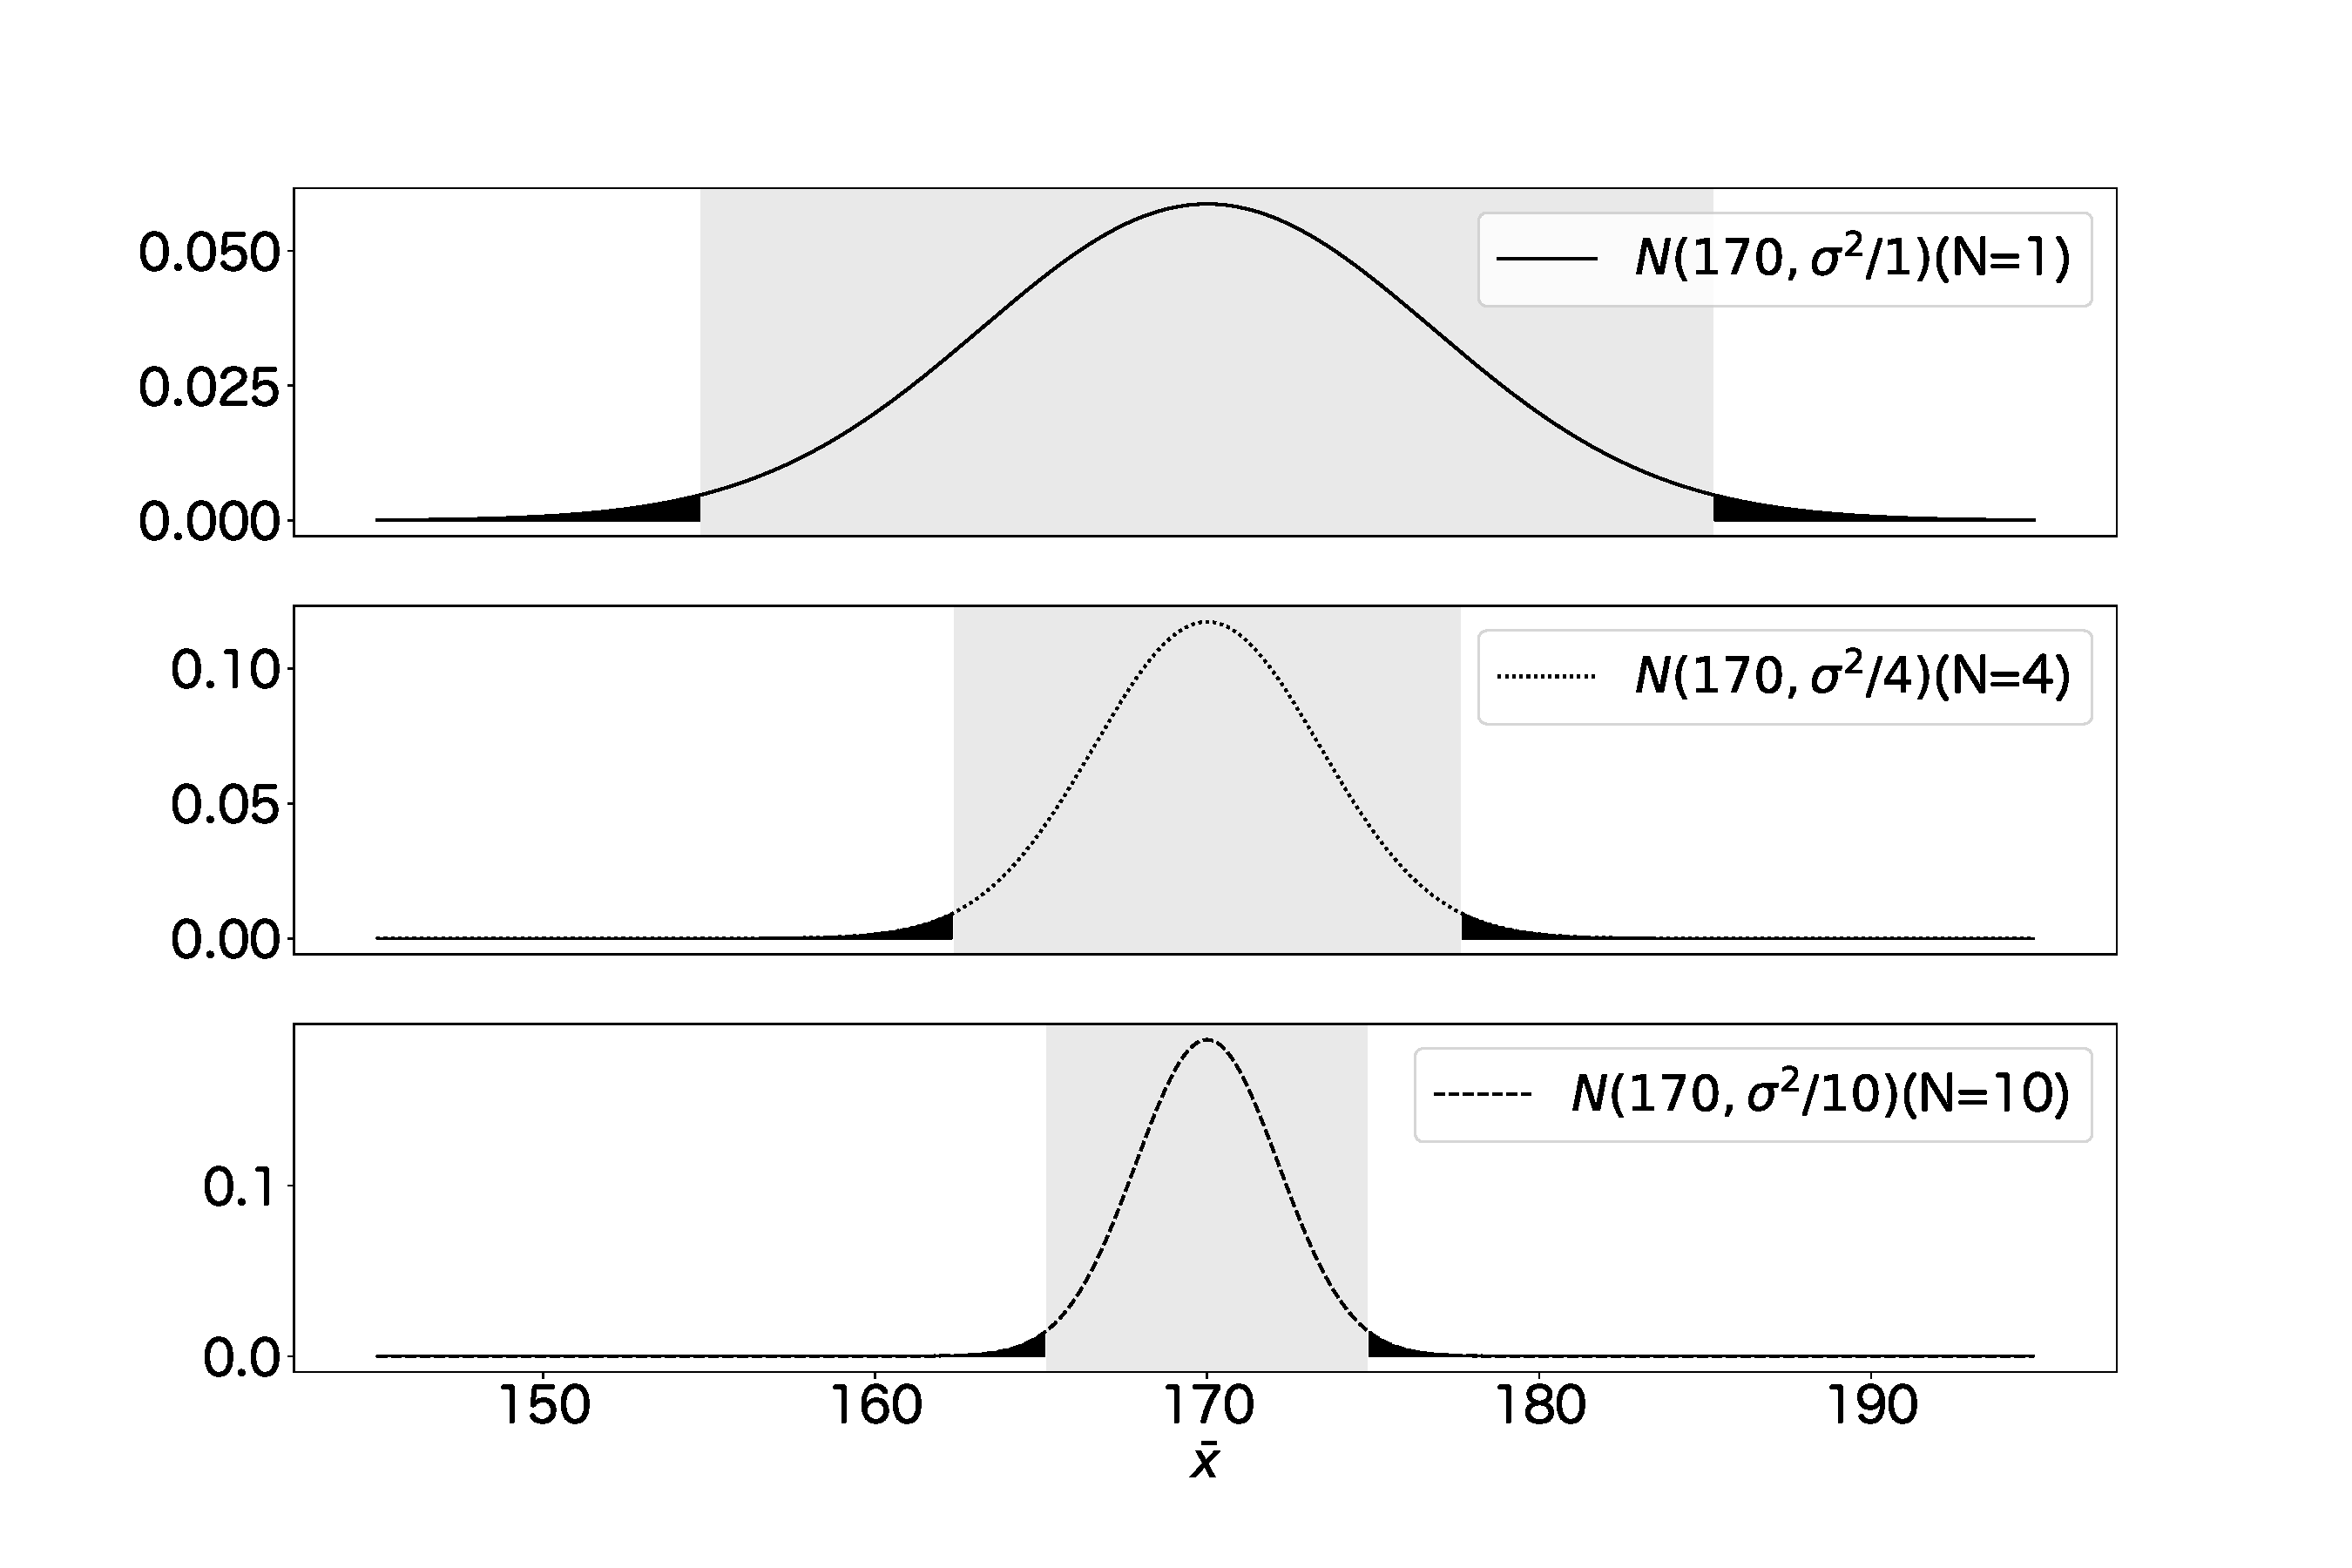
\includegraphics[width=15cm]{./image/03_/confidence_interval.pdf}
%    \caption{信頼区間}
    \caption{(A)$N=1$,(B)$N=4$,(C)$N=10$での信頼区間}
    \label{fig:confidence_interval_n}
  \end{center}
\end{figure}

\if 0
\begin{framed}
    まとめ、
    \begin{itemize}
        \item 統計モデル$M(\mu)$によってサンプリングし、標本を得たとき、標本平均値のよくある値の範囲が信頼区間
    \end{itemize}
    \end{framed}
\fi


\if 0
 川久保統計学P.166
 \fi


%![Z値の頻度]()

信頼区間の中に標本平均が含まれていることは、標本がモデルにり推測可能であることの証拠の一つになる。
ただし、証拠の一つであり、このことは実際には複合的に指標を見て判断する必要がある。
%$\bar{X}$が$95\%$信頼区間の中に入っていることは、この統計モデル
%信頼区間の中に統計量があれば、
%このことから、統計モデル$M(\mu)$でサンプリングしたときに、$95\%$の確率で、この範囲に平均値$\bar{X}$がえられます。


%標本$1$標本$2$について、これを計算してみる。平均値は、それぞれ172.4, 169.0です。
\if 0
標本では、$168.9 < \mu < 176.0$、
この範囲にある$\mu$をもつ統計モデルであれば、この標本によって棄却されない。
%標本$2$では、$165.5 < \mu <172.6$です。
例えば、このモデル$M(\bar{x})$の信頼区間であれば、$M(168)$は棄却できない。
\fi

\if 0
まとめ、
\begin{framed}
    \begin{itemize}
        \item 統計モデル$M(\mu)$のサンプルの平均が$95\%$の確率で入る範囲$\mu - z_{0.025} \frac{\sigma}{\sqrt{n}} < \bar{X} < \mu + z_{0.025} \frac{\sigma}{\sqrt{n}}$。現実の母集団が統計モデルによってよく推測できるなら、この範囲に平均値が入る確率は$95\%$に近くなることもある。逆に、統計モデルが現実をよく捉えることができなければ、母集団から無作為抽出した標本の平均値はこの範囲に入ることは少なくなる。
        \item データがよくある範囲に入る統計モデル$M(\mu)$の$\mu$の範囲$\bar{x}- z_{0.025}\frac{\sigma}{\sqrt{n}} < \mu < \bar{x} + z_{0.025}\frac{\sigma}{\sqrt{n}}$
        \item  統計モデル$M(\mu)$ではサンプルサイズを大きくすると、平均値が入る範囲が狭くなる。
    \end{itemize}
\end{framed}
\fi


\section{指数分布を含んだ統計モデル}
\begin{quote}
    \begin{enumerate}[(1)]
    \item 独立同分布
    \item その分布は、指数分布$(\lambda\exp{(-\lambda x)})$
    \item 指数分布の母数は$\lambda$
    \end{enumerate}
\end{quote}
このモデルを$M_E(\lambda)$とする。
指数モデルにおける$95\%$予測区間は、構成が難しいようなので、省略する\footnote{どうすれば求められるのか、わからない}。
$95\%$信頼区間は式\ref{exp_model_confidence_interval}である。


\subsection{信頼区間を近似する}
$95\%$信頼区間(式\ref{exp_model_confidence_interval})を近似的に求める方法がある。
中心極限定理を使う。このモデルでは、サンプルの平均および分散は、$E[x]=\frac{1}{\lambda},Var[x]=\frac{1}{\lambda^2}$である。このとき、中心極限定理により、$\bar{x}\sim N(E[x],Var[x]/n)$である。よって、$95\%$信頼区間は、
\begin{equation*}
    \frac{1}{\lambda}-z_{0.05}\frac{1}{\sqrt{n}\lambda}<\bar{x}<\frac{1}{\lambda}+z_{0.05}\frac{1}{\sqrt{n}\lambda}
\end{equation*}
である。

解析的に求めた信頼区間と中心極限定理による近似的な信頼区間を比較する(図\ref{fig:model_predict_CI_interval})。
$\lambda=10$としたので、平均は全て$10$である。
$N$が小さいと、解析と近似での信頼区間に差が生じている。近似的な信頼区間は、$0$よりも小さな値も出現することを予測している。平均$10$の指数モデルでは、平均が$0$以下になることはない。このように、モデルの想定しない区間も信頼区間に含めている。
$N$が大きくなると、解析と近似での信頼区間の違いは少なくなる。これは、中心極限定理の帰結から当然である。

\begin{figure}
    \begin{center}
        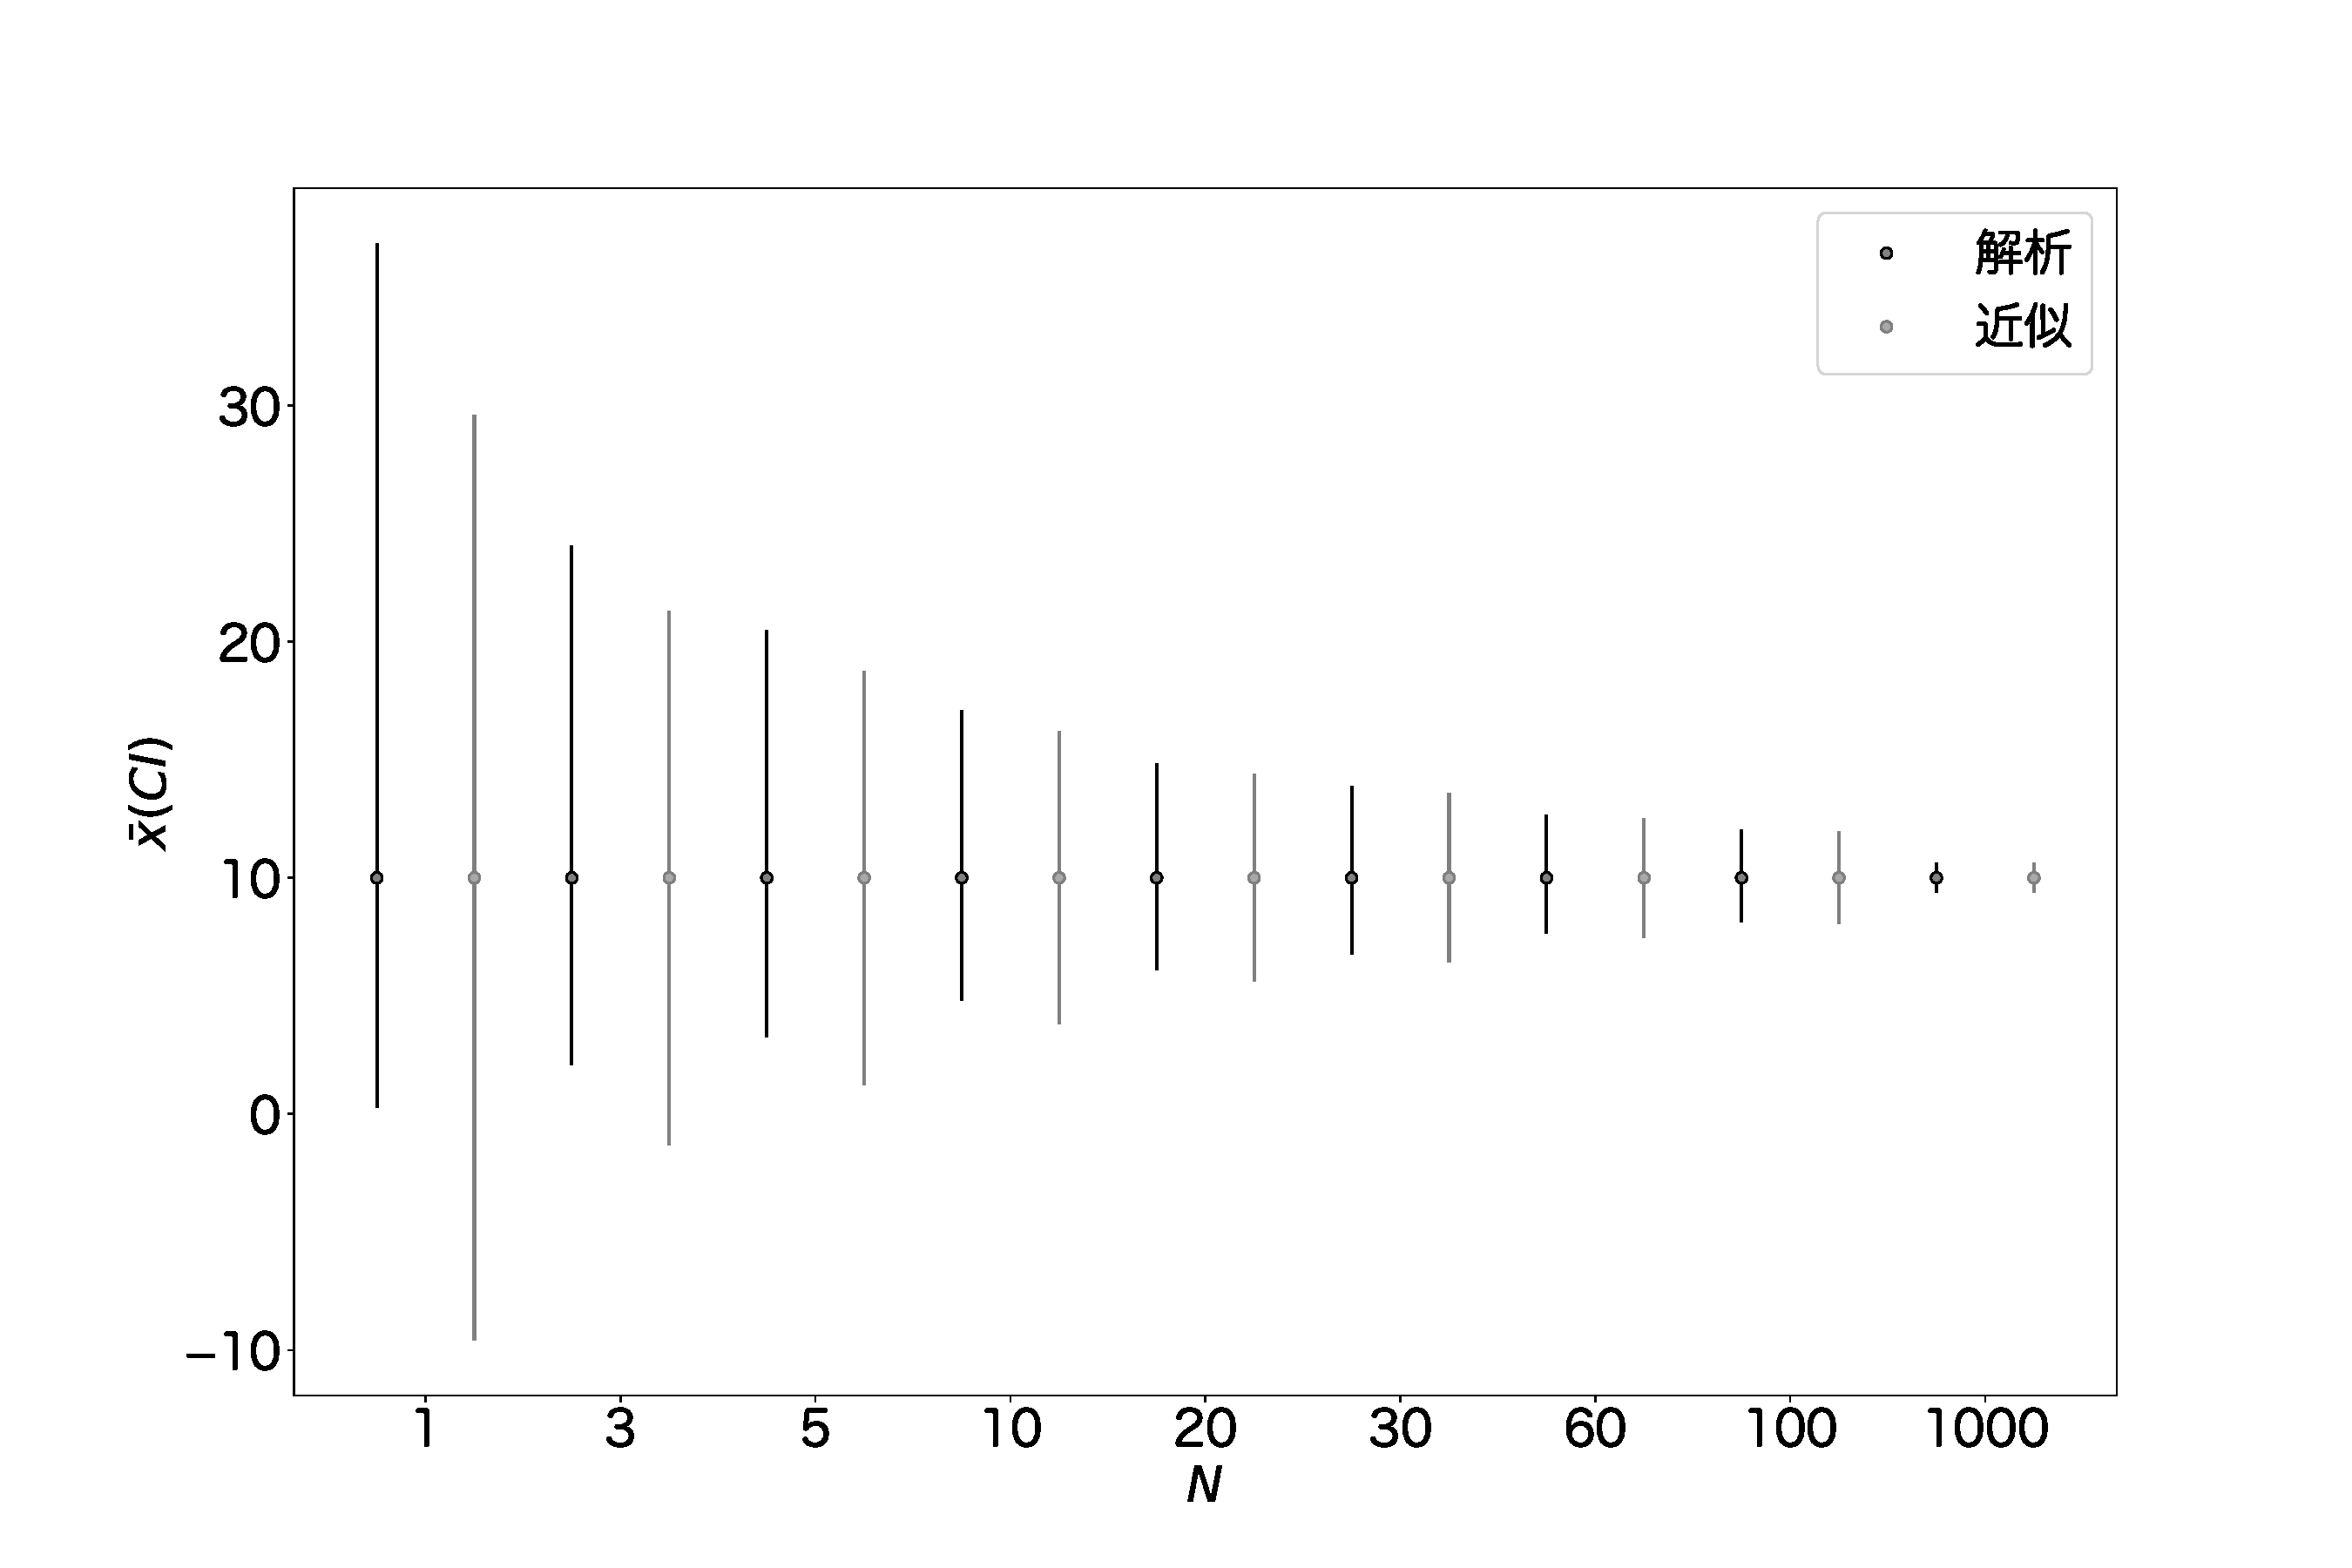
\includegraphics[width=15cm]{./image/12_/confidence_expon_interval.pdf}
        \label{fig:model_predict_CI_interval}
        \caption{解析的な信頼区間と近似によって求められた信頼区間。$1/\lambda=10$とする。横軸にサンプルサイズ。縦軸に、平均値。エラーバーは信頼区間(CI)。}
      \end{center}
    \end{figure}

\section{モデルの選択}
データの分布とモデルの分布が一致しているとき、そのモデルの予測も当たりやすい。
例えば、データがある値の周りに対象に分布していないにもかかわらず、正規モデルを使うと、その予想は当たりにくい。
このことから、データに適したモデルを選ぶ必要があると考えられる。

%ここで、現状のデータからモデルを選択したとして、その予測が当たるかはわからない。
%サンプルサイズが小さいとき、予測が当たりそうなモデルを選ぶことが難しい。
事前実験やこれまでの研究結果から推測し、モデルの分布と標本分布が一致していそうなモデルを選ぶことになる。

モデルを選択できるほどのサンプルサイズを集めて、母集団を予測しやすいモデルを決めることも科学的な成果になりうる。

\subsection{図による比較}
\subsection{AICの比較}

\if 0
\section{標本が統計モデルにより予測可能かを判定する}%統計モデルの性質を使った方法}
%ここまでは、統計モデルの予測がデータと一致することを定量的に評価した。
ここでは、推測に適していないと判断する方法である、統計的仮説検定を紹介する。
この方法は、統計量の一つである統計検定量の統計モデル上での出現しやすさにより、モデルを評価する。
\fi 



\if 0
\section{モデルの種類}

\begin{table}[hbtp]
    \caption{モデル}
    %\label{table:data_type}
    \centering
    \begin{tabular}{ccc}
      \hline
      モデルの仮定  & 棄却域  &  予測区間 \\
      $M(\mu_0,\sigma_0^2)$ $x_1,x_2,\cdots,x_n\sim N(\mu_0,\sigma_0^2)$  \\
      $\mu_0=\bar{x},\sigma_0^2=\frac{1}{n}\sum(x_i-\bar{x})^2$& -  &  - \\
      $\mu_0,\sigma_0$は設定値とする & $\frac{\sqrt{n}|\bar{x}-\mu_0|}{\sigma_0}\sim N(0,1)$  & $\mu_0-z_{\alpha/2}\frac{\sigma}{\sqrt{n}} <\bar{x}<\mu_0+z_{\alpha/2}\frac{\sigma}{\sqrt{n}}$ \\
      $\mu_0$は設定値,$\sigma^2$は未知 & 
      $|\frac{\bar{x}-\mu_0}{\frac{U}{\sqrt{n}}}| > t_{n-1,\frac{\alpha}{2}}$ただし、$U^2=\frac{1}{n-1}\sum(x_i-\bar{x})$
      %$\mu_0=\bar{x},\sigma_0^2=\frac{1}{n}\sum(x_i-\bar{x})^2$ 
      &  \\
      
      \hline
    \end{tabular}
  \end{table}
  \fi
%\chapter{統計量を使ったモデルとデータの比較}
\chapter{モデルにおける統計量の性質}
統計モデルからサンプリングを行った標本から、統計量を計算すると、その統計量より偏った値が出現する確率が得られる。この性質を利用して、モデルからサンプリングを行った標本について、統計量がより偏った値が一定値を下回るならば、このモデルからサンプリングされていないと判定を下し、ある特定の値より大きいならば、このモデルから得られた標本であると判断を下す。

%この確率が低いとき、標本がモデルからサンプリングされたものではないと一定の割合で判断を下すことにする。
%このことを利用して、標本をモデルからサンプリングしたと判断するものとそうでないものに仕分けを行う。

%言い換えるなら、ある母数を持つ統計モデルから標本がサンプリングされたのかい?そうじゃないのか?どっちなんだい?に答える方法の一つである。
%これを科学においては、ある母数をもつ統計モデルによって推測してもいいのかい?そうじゃないのかい?どっちなんだい?統計モデルが「ピー」と答える。
%\footnote{本章で説明する仮説検定とは、前者がモデルとの乖離の程度を調べる方法であり、後者は仮説の真偽を調べる数学的方法という点で完全に異なる。}。



\section{自己標本の批判}
統計モデルからサンプリングした標本の統計量が従う確率密度関数が理論的に求められる。
正規モデルの場合、以下の通りである。
\begin{equation*}
    Z = \frac{\sqrt{n}(\bar{x}-\mu)}{\sigma} \sim N(0,1)
\end{equation*}
この性質を利用することで、$Z$値よりも偏った値がどの程度の確率で出現するかが計算できる。
例えば、$Z=0$であれば、モデル内でこれ以上に偏った値が出現する確率は約$0.5$程度であり、よくある値であることがわかる。
一方、$Z=1.96$であれば、モデル内でこれ以上に偏った値が得られる確率は約$0.025$程度となり、なかなかレアな値であると思うことができる。
%ここで注意しなければならないのは、$p$値はモデル内における$Z$値よりも偏った値の出現する確率であるということである。
%言い換えれば、現実において$Z$値よりも偏った値の出現する確率についてはなんら言及できていない。
%統計量以上に偏った値がモデルにおいて出現する確率を$p$値という。



\begin{defi}
    統計モデルにおいて、その標本の統計量よりも偏った(大きいまたは小さな)値が得られる確率を$p$値と呼ぶ。
    %ある標本から求められた統計量以上に大きな値が得られる確率を$p$値と呼ぶ。
    %絶対にダメと判断されないときは、統計モデルを採択(棄却の対義語)すると宣言しない。
    %統計モデルが棄却されるのは、統計モデルの仮定によって変化する。本書の範囲内であれば、統計モデルの母数、分布関数、独立同一の分布関数からサンプリングされたことによる。
    %最尤統計モデルにおいて、棄却されない統計モデルの母数の範囲を信頼区間といい、棄却されるモデルの母数の範囲を棄却域という。
\end{defi}

あるモデルでの標本の得られにくさを、$p$値に変換して検討することが可能である。
$p$値が小さいなら、統計量$Z$値以上に偏った値の得られる確率が低いということであるので、
$Z$値の元の標本もそもモデルからは得られにくいということを示す。
%つまり、モデルから標本の得られにくさの指標の一つが$p$値であるとも言え、$p$値が小さいほど、その標本はそのモデルから得られにくい。

\if 0
\begin{center}
    標本$\rightarrow$ 統計量 $\rightarrow$ $p$値($p$値の小ささが標本のモデル上での得られにくさの指標になる)
\end{center}
\fi




\subsection{$p$値の計算練習}
%$Z(\bar{x},\mu)$以上の値が得られる確率}
$Z(\bar{x},\mu)\sim N(0,1)$により、$Z$以上の値が得られる確率の計算を練習してみよう。つまり、以下をコンピュータに計算させる。
\begin{equation*}
    p = \varPhi(Z(\bar{x},\mu)>x)
\end{equation*}
正規モデル$M(\mu=168;\sigma^2=6.8)$から得た標本の統計量を、$\bar{x}=172.4$、サンプルサイズを$n=10$とする。
$Z$値は$Z(\bar{x},\mu)=2.04$となる。これを元に、以下のスクリプトを実行すると、$p$値が約0.04程度であることがわかる。

\begin{lstlisting}
xbar = 172.4
mu = 168
sigma2 = 6.8**2
n=10
Z = np.sqrt(n)*(xbar-mu)/np.sqrt(sigma2)
print(Z)
p=1-norm.cdf(Z,0,1)
print(p*2)
\end{lstlisting}



\subsection{自己標本の否定確率}
%ここから、いくつか数学的な構造について紹介する。
%この内容は科学において使うのは非常に難しい。
%例えば、有意水準$\alpha$や検定量$\beta$などを決定することはできない。
%$Z_i$がモデル由来であるかを自己標本の批判を元に判断する。

正規モデル$M$において、$M$の標本を得てその統計検定量Zが極端な値を取るとき、$M$の標本ではないと判定する。
ここで、極端な値とは、$Z$が標準正規分布に従うことから、標準偏差の2よりも偏った値である場合に、$M$の標本ではないとする。
このとき、標準正規分布表を参照すれば$P(|Z|>2)=0.02275\times 2=0.046$程度となる。

標準偏差の代わりに確率を元に判定を行う。
$P(|Z|>x)=0.046$はキリが悪いので代わりに、$P(|Z|>x)=0.05$を設定する。
標準正規分布表を参照すれば$P(|Z|>x)=0.05$となるのは$x=1.96$程度である。
この値よりも大きな$|Z|$となる標本は、$M$の標本ではないと判定する。

あるモデルの統計検定量がより偏った値を取る確率$0.05$を他の統計モデルでも適用すれば、さまざまなモデルで統一的に判定が行える。また、あるサンプルサイズの標本をモデルから100回サンプリングした場合、$95$回はモデルから生成されたものと判断され、残りの5回についてはモデルから生成されていないと判断することになる。


\begin{defi}
    モデルからサンプリングされた標本のうち、モデルから生成されたものではないと判定する割合を$\alpha$とし、有意水準と呼ぶ。
    言い換えれば、$\alpha$値は、統計モデルからサンプリングされた値について、これが元の統計モデルからサンプリングであることを判定する閾値\footnote{閾値(読み:いきち)=限界値}である。
\end{defi}

%本書では、上記の歴史的な事情にしたがって、$\alpha=0.05$を利用して、理論計算を行う。


\begin{SMbox}{有意水準は$0.05$でよし}
    よくある受け答えを引用しておく\cite{greenland2016statistical}。
    \begin{quote}
        Q: Why do so many colleges and grad schools teach p = 0.05?

        A: Because that's still what the scientific community and journal editors use.

        Q: Why do so many people still use p = 0.05?

        A: Because that's what they were taught in college or grad school.
    \end{quote}
\end{SMbox}
%これは、モデル$M$の標本であるはずなのに、外れた値であれば、そのモデル$M$
%モデルが生成したはずの標本であるが、閾値を決めてモデルから生成されたものではないとするのである。
%モデルが自身から得られた標本を批判するのであるから、自己の標本を批判するのである。
%これは、モデルを元に、標本がモデルにより予測できるかどうかを考えている。


%具体的には、正規モデルを利用すれば、その統計量$Z$が$N(0,1)$に従うことがわかっている。
%$Z$の値が偏った値になっていれば、その出現頻度は低くなるので、$P(|z|<Z)=95/100$となる$Z$を計算する。
%この$Z$は具体的に計算でき、$Z_{0.95}=1.96$である。
%ここから、$|z_i|<Z_{0.95}=1.96$となる$z_i$の個数を数えればおよそ$95$になる。
%また、$|P(|z_i|>0.95)| > 1.96$ならば、$|z_i|>Z_{0.95}=1.96$である。
\if 0

\fi

%統計モデルの分布関数が変化すれば、その統計モデルにおける信頼区間・棄却域の値も変わる\footnote{中心極限定理を利用し、統計量の出現範囲を近似することが多い。}。
%実際のデータが$\alpha\%$の割合で棄却されるということではない。モデルから生成された標本であるのに、この統計モデルから生成されていないと疑いをかける。

\subsection{$\mu$の変化に応じた信頼区間}
%$95\%$信頼区間と$p$値の関係}
正規モデル$M$においてその統計検定量$Z$について、式変形を行なう。
\begin{eqnarray}
    & &|z| > Z_{0.95}( = 1.96 ) \notag \\
    &\rightarrow& \frac{\sqrt{n}|\bar{x}-\mu|}{\sigma} > Z_{0.95} \notag\\
    &\rightarrow& \mu-\frac{\sigma}{\sqrt{n}}Z_{0.95} < \bar{x} < \mu+\frac{\sigma}{\sqrt{n}}Z_{0.95} \label{confidence_interval_eqn}
\end{eqnarray}
\begin{defi}
式\eqref{confidence_interval_eqn}の$\bar{x}$の区間を信頼区間といい、次の式で定義される。
\begin{equation*}
    A=\{x;\mu-\frac{\sigma}{\sqrt{n}}Z_{0.95} < x < \mu+\frac{\sigma}{\sqrt{n}}Z_{0.95} \}
\end{equation*}
これ以外の区間を棄却域と言う。ここでは、$R=\mathbb{R}\backslash A$が棄却域である。
% Comment
%信頼区間の定義は、統計検定量の範囲ではなく、平均値の範囲
\end{defi}
信頼区間の範囲は、サンプルサイズ$n$、有意水準$\alpha$およびモデルの母数$\mu,\sigma^2$により決まる。
$\mu$の変化に応じて、信頼区間が変化する様子を確かめる。

図\ref{fig:confidence_interval_model}には、モデル毎の平均値と信頼区間を描いた。$\mu$の大きさにによらず信頼区間の幅は同じである。
各$\mu$に対して、信頼区間の内側で$\bar{x}$が$95\%$の確率で見つかることを統計モデル$M(\mu)$が推測する。
この外側にある$\bar{x}$になる標本については統計モデルの標本ではないと判定を下す。

\begin{figure}
    \begin{center}
        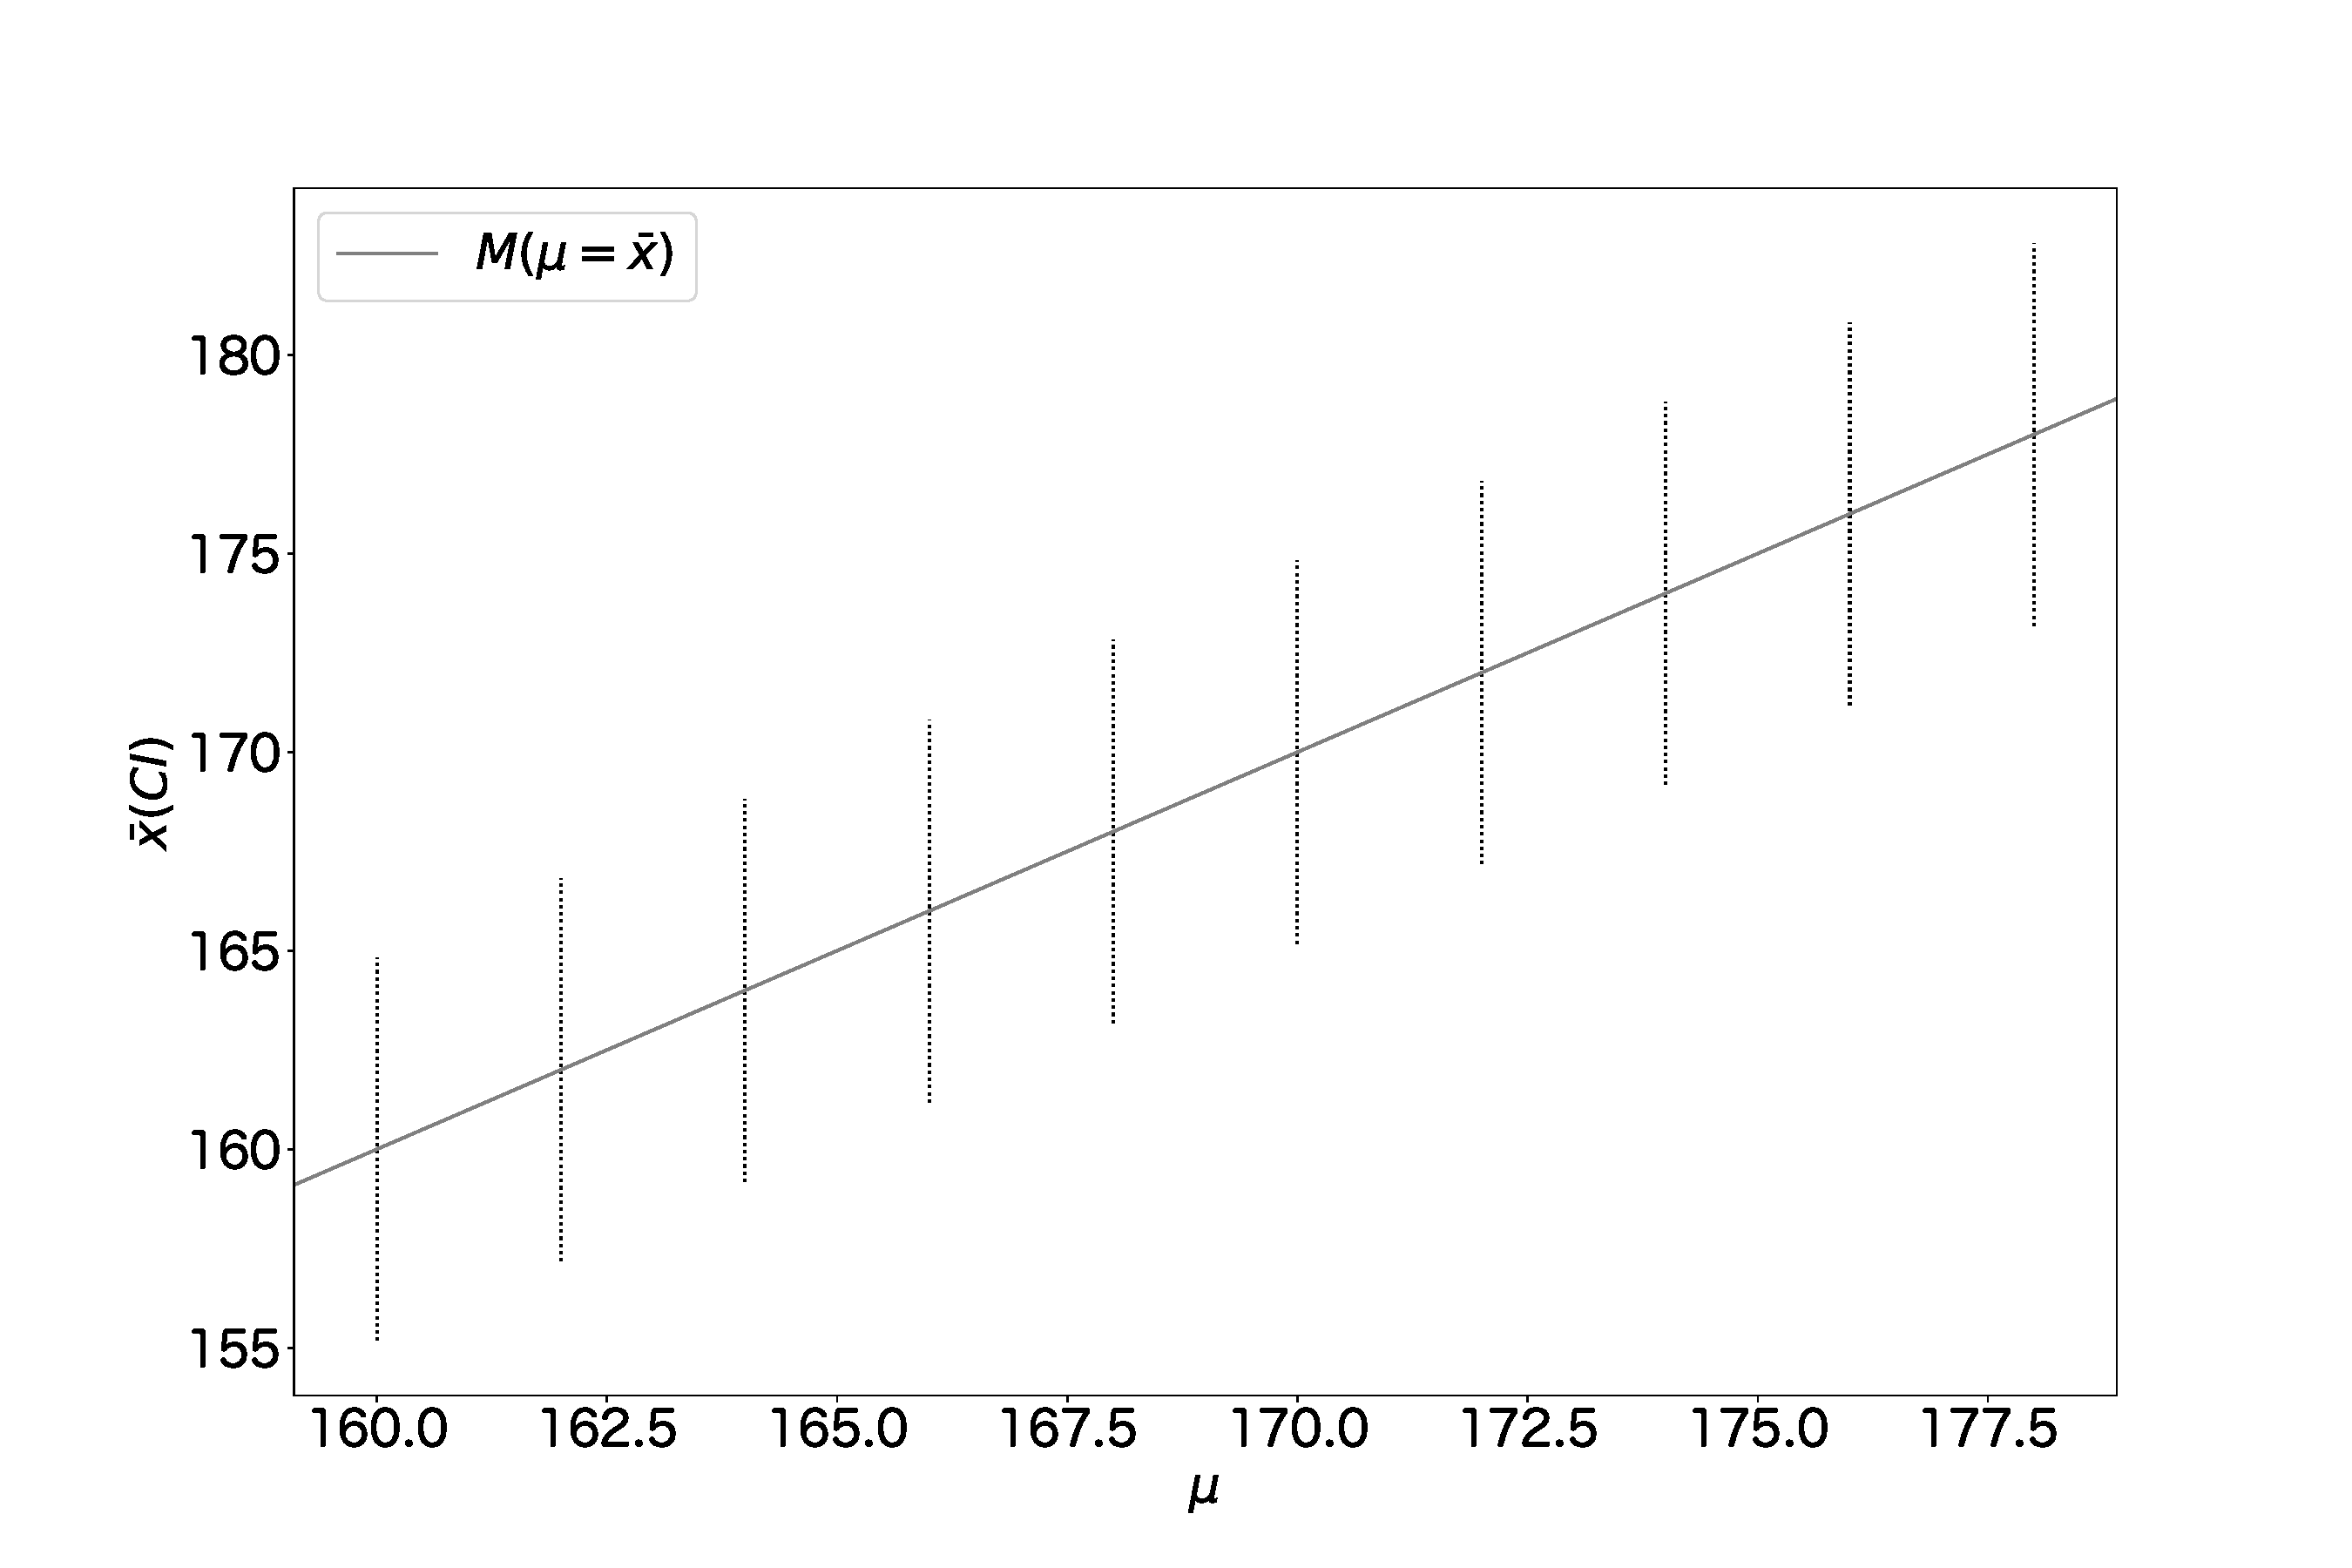
\includegraphics[width=10cm]{./image/04_/confidence_interval_model.pdf}
        \caption{横軸にモデルの母数$\mu$、縦軸に、モデルが予測する平均値$\bar{x}$、エラーバーに$95\%$信頼区間を描いた。$N=10,\sigma^2=6.8^2$}
        \label{fig:confidence_interval_model}

    \end{center}
\end{figure}



\section{統計量をもとにしたモデル間類似度(検出力)}
母数の異なる二つの統計モデル$M_a,M_b$について考察する。
$M_a$の信頼区間内の統計量が$M_b$において出現する確率を検出力という。
言い換えれば一方で出現する統計量が他方のモデルにおいて出現する確率である。
これは、$M_a$から$M_b$へのモデル間の統計量を元にした類似度と言える。

\subsection{検出力の定義}
$M_a$信頼区間$A$が$M_b$において出現する確率を$\beta$とする。$\beta$を検出力という\footnote{検出力を検定力または統計力と呼ぶこともある。\\ \url{https://id.fnshr.info/2014/12/17/stats-done-wrong-03/}}。

具体的には以下の式で表される。
\begin{eqnarray*}
    & &P_a(x \in R_a) = \alpha\\
    & & P_b(x \in A_a) = P_b(x\notin R_a )=\beta
\end{eqnarray*}
ここで、$R_a,A_a$はそれぞれ統計モデル$M_a$の棄却域、信頼区間を表し、$P_a,P_b$は、それぞれ統計モデル$M_a,M_b$におけるある統計量がしたがう分布の密度関数。

検出力$\beta$は、二つの異なるモデルを比較するための指標である。
二つの統計モデルの母数がよく一致するならば、$\beta$は$1-\alpha$に近い値を取る。一方、一致していないならば、$\beta$は0に近い値を取る。
また、$M_a$に対する$M_a$の検出力$\beta$は、$1-\alpha$である。
%$M_a$を棄却する閾値を低く設定すると、$\beta$は大きな値になる。

\subsection{正規分布モデルの検出力}
具体的に、$P_a(x \in R_a),P_b(x \in A_a)$を計算してみる。

$\sigma^2$がすでに与えられた正規モデルを$M(\mu)$とし、$M_a=M(\mu_a),M_b=M(\mu_b)$とする。
$M_a$または、$M_b$からサンプリングされた確率変数$x_1,x_2,\cdots,x_n$の平均値は、それぞれ$\bar{x}_a\sim N(\mu_a,\sigma/n)$または$\bar{x}_b\sim N(\mu_b,\sigma/n)$である。
$M_a$の信頼区間$A_a$は、$|\bar{x}_a|<\mu_a+\sigma / \sqrt{n}z_{2.5\%}$である。
このとき、$P_a$を$N(\mu_a,\sigma)$の確率密度関数とすると、
\begin{equation*}
    P_a(x \in A_a) = 1-\alpha
\end{equation*}
であるのは定義から明らか。
また、$P_b$を$N(\mu_b,\sigma)$の確率密度関数とすると、
\begin{equation*}
    P_b(x \in A_a ) = \beta
\end{equation*}
である。
モデルの母数平均$\mu_a$と、$\mu_b$が一致していれば、$P_b(x \in A_a )$も$1-\alpha$に近くなる。
$\mu_b$が$\mu_a$から離れていくと、$P_b(x \in A_a)=0$に近づいていく。


\begin{figure}
\begin{center}
    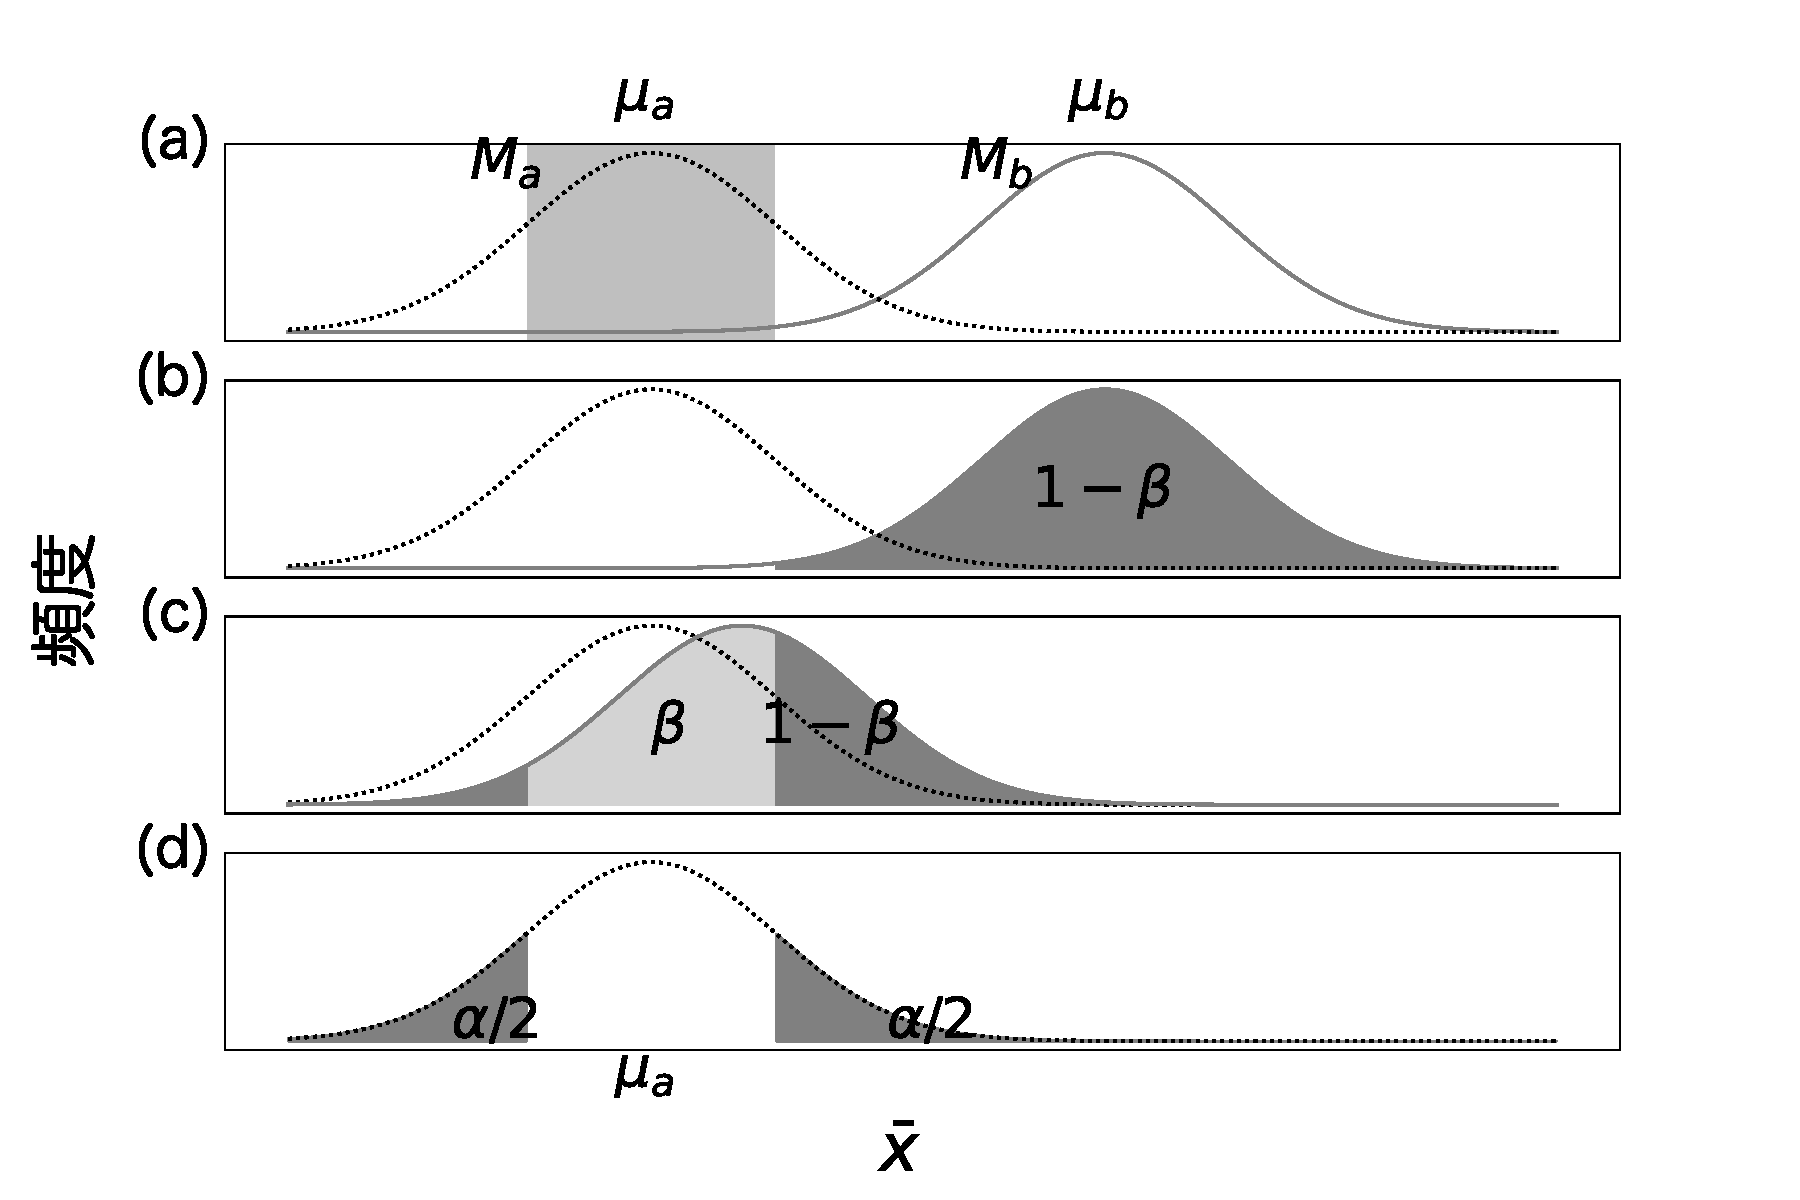
\includegraphics[width=15cm]{./image/04_/power_of_a_test_2.pdf}
    \caption{統計モデル$M_a,M_b$から計算された統計量$\bar{x}$の確率分布$P_a,P_b$。(a)灰色の範囲は$M_a$の信頼区間。(b)灰色の領域は、$1-\beta$の領域を示している。$\beta$の領域が小さいので、描画できなかった (c)$\mu_b$が$\mu_a$に近いときの$\beta$と$1-\beta$の領域。(d)灰色の範囲の面積が$\alpha$を示している。}
    \label{fig:power_of_test_alpha_beta}
\end{center}
\end{figure}


検出力と$\alpha$の領域を図示した(図\ref{fig:power_of_test_alpha_beta})。$M_a$の$95\%$信頼区間は、$|\mu|<\mu_a+z_{0.025}\frac{\sigma}{\sqrt{N}}$である。信頼区間は、図\ref{fig:power_of_test_alpha_beta}(a)において灰色で塗った$x$軸の範囲である。$\alpha$は図\ref{fig:power_of_test_alpha_beta}(c)の灰色で塗りつぶした領域の面積である。
検出力$1-\beta$は、$M_b$における$M_a$の信頼区間の外側の領域の面積なので、図\ref{fig:power_of_test_alpha_beta}(b)の濃い灰色の範囲である。

$\alpha$を0に近づけていくと、信頼区間は徐々に大きくなり、$\beta$は大きくなる。
$\alpha$を1に近づけていくと、信頼区間は徐々に狭くなり、$\beta$は小さくなる。



\begin{figure}
    \begin{center}
        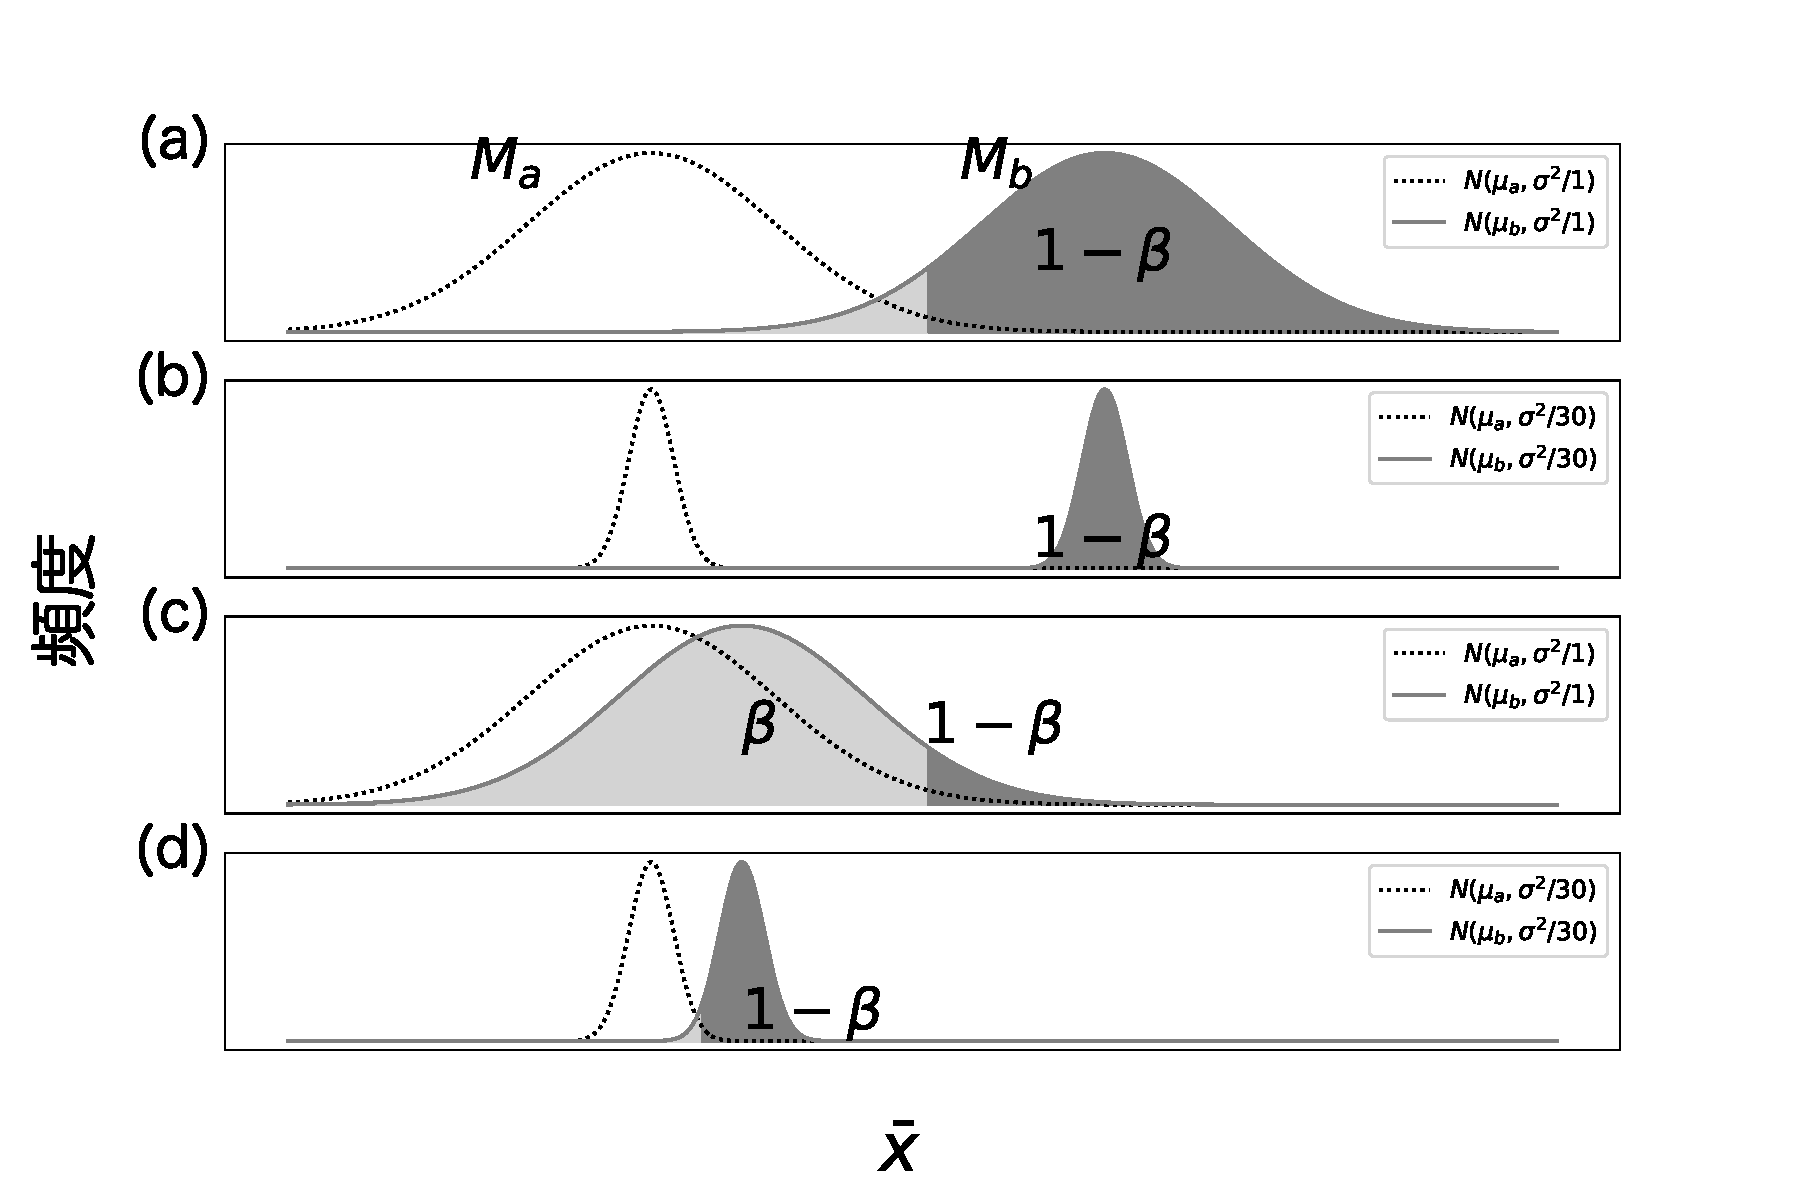
\includegraphics[width=15cm]{./image/04_/power_of_a_test_3.pdf}
        \caption{統計モデル$M_a,M_b$から計算された統計量$\bar{x}$の確率分布$P_a,P_b$。(a)$\mu_a,\mu_b$のサンプルサイズ$1$の平均値がしたがう確率密度関数$N(\mu_a,\sigma^2/1),N(\mu_a,\sigma^2/1)$。(b)(a)と同じ$\mu_a,\mu_b$に対して、サンプルサイズを$30$にした場合の確率密度関数。(c)$\mu_a,\mu_b$が(a)よりも近いときの$\bar{x}$の確率密度関数。(d)(c)と同じ$\mu_a,\mu_b$に対してサンプルサイズを$30$にした場合の$\bar{x}$の確率密度関数。}
        \label{fig:power_of_test_alpha_beta_sample_size}
    \end{center}
    \end{figure}

    

$\alpha$、$M_a$の母数平均$\mu_a$、$M_b$の母数平均$\mu_b$を固定したまま、サンプルサイズを変化させ,
$\beta$の変化を表す(図\ref{fig:power_of_test_alpha_beta_sample_size})。$\bar{x}$の確率密度関数($N(\mu,\sigma^2/n)$)の分散がサンプルサイズによって変化することは明らかである。このことから、サンプルサイズが大きくなると、信頼区間は徐々に狭くなり、$1-\beta$は大きくなる。サンプルサイズが小さいときは、$1-\beta$も小さくなる。

$\mu_a$を固定し、$\mu_b$を変化させたときの検出力$1-\beta$を図\ref{fig:power_of_test_N_mu0_variable}に示した。
サンプルサイズが大きければ、$1-\beta$も大きくなることがわかる。

\begin{figure}
    \begin{center}
        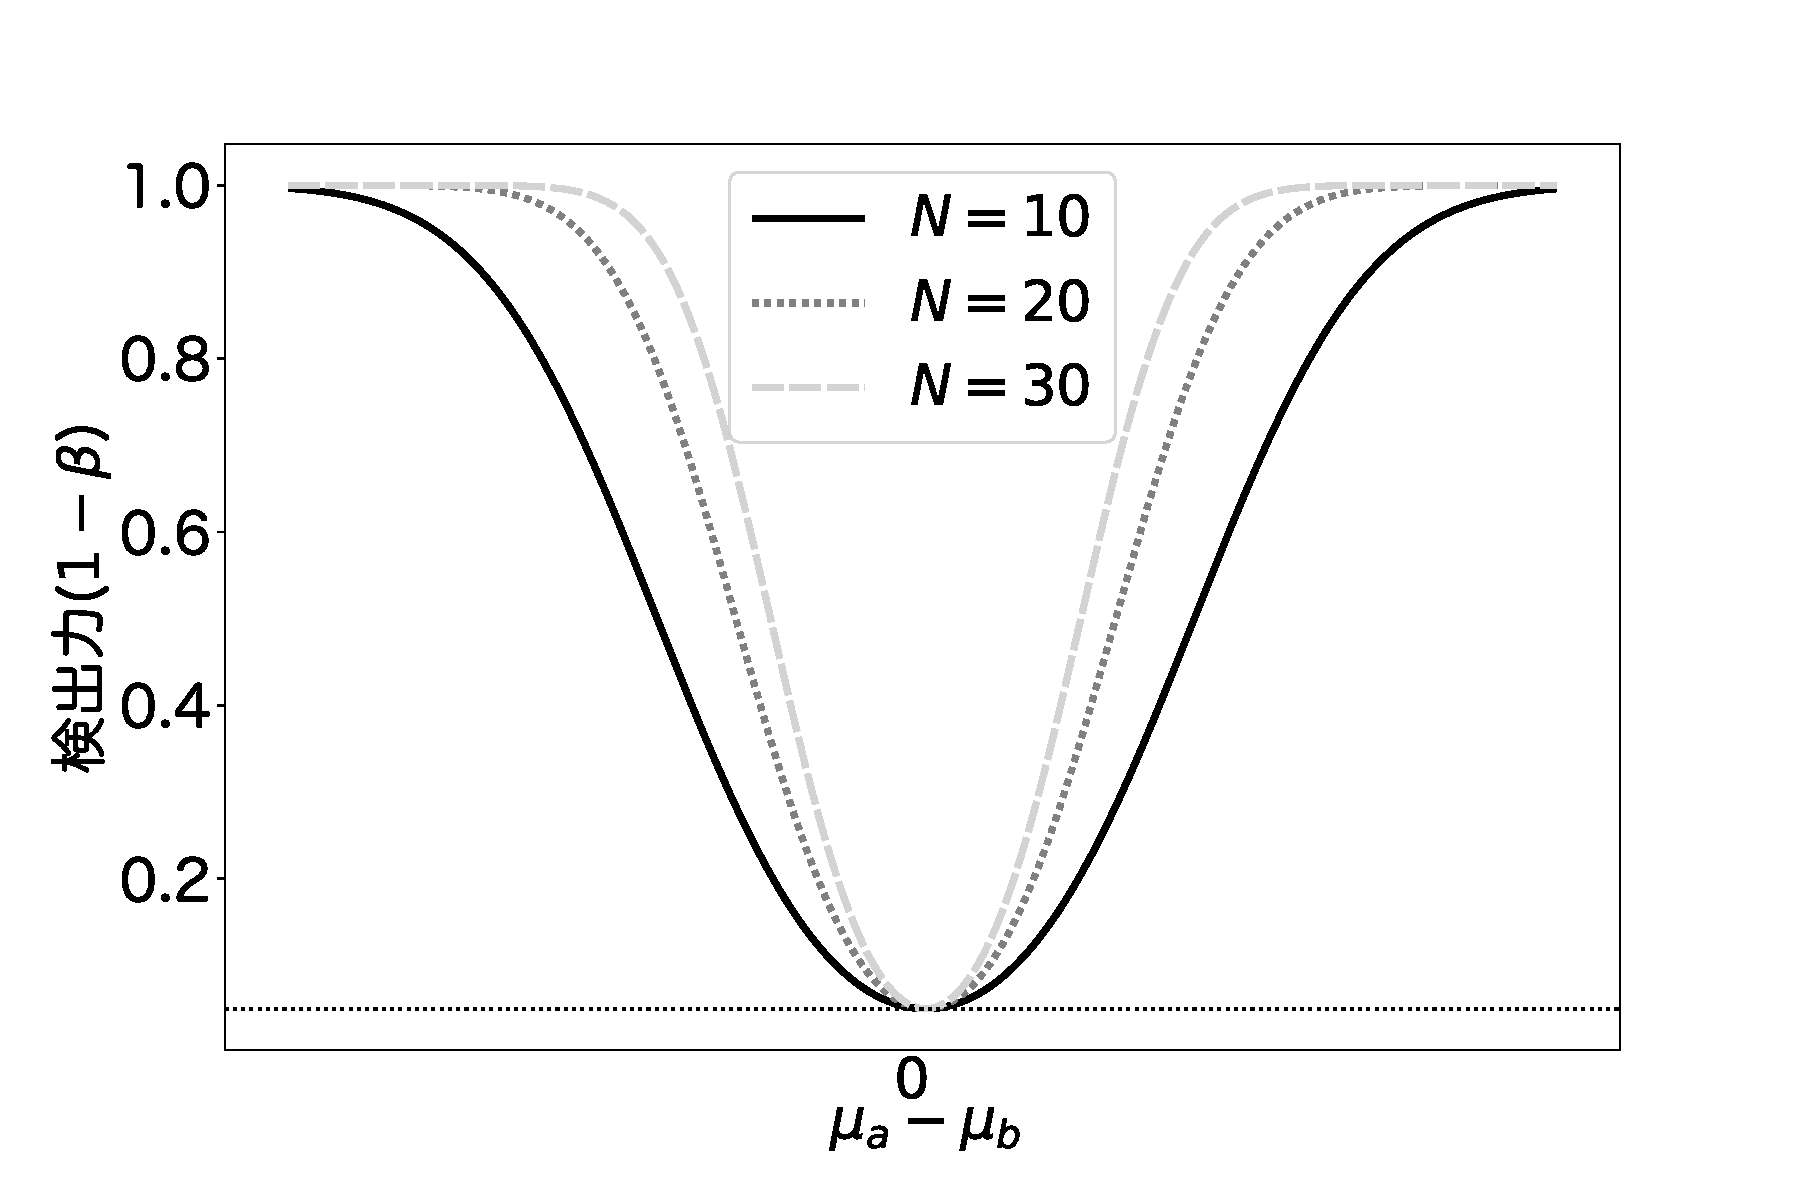
\includegraphics[width=15cm]{./image/04_/power_of_test.pdf}
        \label{fig:power_of_test_N_mu0_variable}
        \caption{$\mu_a$を変数にしたときの検出力(検出力関数)。}
    \end{center}
\end{figure}

$\beta$を定義したことにより、$\beta$の数値を決定し、$M_a,M_b$の違いが$\beta$になるために必要なサンプルのサイズが推測できる。ここでは、$\mu_a,\mu_b$が固定されている状況を考える。
検出力$1-\beta$は$1$に近いほど、$M_a,M_b$が違うと主張できる。
あらかじめ決めたおいた基準の$1-\beta$を閾値を設定し、それ以上の$1-\beta$となるサンプルサイズを推測する。
サンプルサイズが小さければ、$M_a$と$M_b$の違いは曖昧であり、サンプルサイズが大きくなると、はっきりとモデルの違いがわかる。




\subsection{$\beta$の計算}
正規モデル$M_a,M_b$を使って、$\beta$を計算してみる。
$M_a$の信頼区間は、
\begin{equation*}
    -z_{0.025}\leq \frac{\sqrt{n}(\bar{x}-\mu_a)}{\sigma}\leq z_{0.025}
\end{equation*}
より、
\begin{equation*}
    A_a = \{ x ; \mu_a -\frac{\sigma}{\sqrt{n}}z_{0.025} \leq x \leq \mu_a +\frac{\sigma}{\sqrt{n}}z_{0.025} \}
\end{equation*}
である。ここで、$a=\mu_a -\frac{\sigma}{\sqrt{n}}z_{0.025},b = \mu_a +\frac{\sigma}{\sqrt{n}}z_{0.025} $とおく。棄却域は$A_a$以外の$\mu$である。$M_b$の標本平均$\bar{x}_b$は、$N(\mu,\frac{\sigma^2}{n})$に従うので、$A_a$の区間で、$N(\mu_b,\frac{\sigma^2}{n})$の面積を計算すれば良い。
ここで、$\frac{\sqrt{n}(\bar{x}_b-\mu_b)}{\sigma}\sim N(0,1)$である。
このことを利用すると、
$a,b$は、$N(\mu_b,\frac{\sigma^2}{n})$の確率変数だとすると、
\begin{eqnarray*}
    A &=& \frac{\sqrt{n}(a-\mu_b)}{\sigma} \\
    %&=& \frac{\sqrt{n}(\mu_a-\frac{\sigma}{\sqrt{n} z_{\alpha/2}})}{\sigma}\\
    &=& -z_{\alpha/2}+\frac{\sqrt{n}}{\sigma}(\mu_a-\mu_b)
\end{eqnarray*}
同様に、
\begin{eqnarray*}
    B &=& \frac{\sqrt{n}(b-\mu_b)}{\sigma} \\
    %&=& \frac{\sqrt{n}(\mu_a-\frac{\sigma}{\sqrt{n} z_{\alpha/2}})}{\sigma}\\
    &=& z_{\alpha/2}+\frac{\sqrt{n}}{\sigma}(\mu_a-\mu_b)
\end{eqnarray*}
である。以上より、確率密度関数$N(0,1)$において、$-z_{\alpha/2}+\frac{\sqrt{n}}{\sigma}(\mu_a-\mu_b) \leq x\leq  z_{\alpha/2}+\frac{\sqrt{n}}{\sigma}(\mu_a-\mu_b)$の間で積分すれば良い。

$d=\frac{\mu_a-\mu_b}{\sigma}$とおく。$d=0.6,n=9$とする。このときの$\beta$を計算してみる。$N(0,1)$において、$-z_{\alpha/2} -0.6\sqrt{n} \leq x \leq z_{\alpha/2} +0.6\sqrt{n}$の区間で積分する。

\begin{lstlisting}
A,B = norm.interval(0.95,0.,1)
N = 9
d = 0.6
a,b = A+d*np.sqrt(N),B+d*np.sqrt(N)
print(a,b)
norm.cdf(b,0,1)-norm.cdf(a,0,1)
\end{lstlisting}

答えは、$0.564$


\subsubsection{サンプルサイズ}
$d$と検出力を指定したときに、$M_a,M_b$の類似度を検出力以上にするためのサンプルサイズが計算できる。
$\beta=0.1,\d=0.8$とし、この$\beta$を満たすように$N$を計算した。

\begin{lstlisting}
A,B = norm.interval(0.95,0.,1)
beta = 0.1
d = 0.8
for N in range(10,200,2):
    a,b = A+d*np.sqrt(N),B+d*np.sqrt(N)
    beta_ = norm.cdf(b,0,1)-norm.cdf(a,0,1)
    if beta_ < beta:
        break
print(N)
\end{lstlisting}
サンプルサイズは、$18$であることがわかる。



\subsection{最尤モデルでの$\beta$の計算}
\subsubsection{データを元にしたモデルとモデルの類似度}
統計モデルAを$M(\mu=170)$とし、統計モデルBを$M(\bar{X})$とする。ここで、$\bar{X}$は、無作為抽出によって得られた標本の平均であり、標本の大きさを$100$とする。
モデルA,Bの間の検出力が計算可能である。
$d=\frac{170-\bar{X}}{6.8}$、$n=100$であるので、$\bar{X}=168$を得たとすると、
\begin{lstlisting}
A,B = norm.interval(0.95,0,1)
N = 100
d = (170-168)/(6.8)
a,b = A+d*np.sqrt(N),B+d*np.sqrt(N)
print(a,b)
norm.cdf(b,0,1)-norm.cdf(a,0,1)
\end{lstlisting}
その検出力は、$0.163$


\section{過誤}
これまでの議論をまとめる。モデル$M_a$からサンプリングを行った標本について、モデル$M_a$に関する標本であるかを判定する。モデルから生成された標本であるが、偏った統計量出会った場合は、モデルから生成されていないと判断する。この頻度を$\alpha$とした。このように、モデル$M_a$から生成されたのに、統計量の出現頻度から、このモデルから生成したものではないと言う誤った判断を行う事になる。このことを判断の間違いであると言うことから第1'の過誤と呼ぶ。

次に、モデル$M_b$からサンプリングによって得られた標本が、別のモデル$M_a$からサンプリングされものであるかどうかを判定することを考える。この場合、統計量が信頼区間含まれているかどうかを確認し、含まれていない場合には、モデル$M_a$からサンプリングされた標本ではないと判定できる。問題は、統計量が信頼区間に含まれている場合である。この場合、実際には、$M_a$からサンプリングされていないのにもかかわらず、誤って$M_a$からサンプリングされた標本であると判断することになる。この誤った判断を第2'の過誤と呼ぶ\footnote{Neyman-Pearsonとは異なる過誤を定義したので、1'および2'とした。仮説検定において、Neyman-PearsonとFisherを混ぜ合わせて過誤を定義することが現在の主流である}。以上のことをまとめると、表\ref{table:type_error}のようになる。

\begin{table}[hbtp]
    \caption{モデル$M_a$による自己標本批判}
    \label{table:type_error}
    \centering
    \begin{tabular}{ccc}
      \hline
        &  $M_a$の信頼区間に &  $M_a$の信頼区間に \\
        & 標本の統計量が入っていない & 標本の統計量が入っている \\
      \hline \hline
      モデル$M_a$の標本  & モデル$M_a$の標本ではないと判定  & モデル$M_a$の標本と判定 \\
      & (第1'の過誤) & \\
      モデル$M_b$の標本  & モデル$M_a$の標本ではないと判定   & モデル$M_a$の標本であると判断 \\
      & & (第2'の過誤) \\
      \hline
    \end{tabular}
  \end{table}


\begin{SMbox}{正解と回答の違い}
    あるデータ群に対してそのデータの特徴を元に、YesまたはNoとアノテーションをつける。
    データからそのYesまたはNoを予測する手順を開発する。
    その手順によって得た回答と、正解(真の値)の一致と不一致は以下の通りになる(表\ref{table:Yes_no_answer})。
    回答と一致したら、True、一致しないならFalse。
    Yesと予測したらPositive、Noと予測したらNegativeとする。
    回答がYesな問題に、Yesと答えることは(手順が正しい予測を行なった)、True Positiveといい、Noと答える(手順が間違えた予測を行なった)ことはFalse Negativeという。回答がNoな問題に、Yesと答えることを、False Positive、また、Noと答えることをTrue Negativeという。

    モデル$M_a$の標本にYesを対応ずけ、モデル$M_b$の標本にNoを対応付ける。標本を元に、YesまたはNoを判定する手順をモデル$M_a$を元にした統計検定を利用する。この問題において回答がFPとなったものを第1'の過誤であり、FNとなったものが第2'の過誤である。
    \end{SMbox}
    
    
    \begin{table}[hbtp]
    \caption{正解と回答の違い}
    \label{table:Yes_no_answer}
    \centering
    \begin{tabular}{ccc}
        %\hline
          &  負例(真の値) & 正例(真の値)  \\
        \hline \hline
        正例(予測値) &  偽陽性(FP)  & 真陽性(TP)\\
        &予測が外れた & 予測が当たった\\
        負例(予測値) & 真陰性(TN) & 偽陰性(FN)\\
        & 予測が当たった & 予測が外れた\\
        \hline
    \end{tabular}
    \end{table}

    


\section{自己否定の過推定}
統計モデルからサンプリングされた標本を、統計量により元のモデルからサンプリングされたかどうかを判断するとき、そのモデルからサンプリングされた標本ではないと想定以上に判断してしまうことがある。
このような過度な推定は、二つの要素に分解できる。
不適切な統計量を使用することで、棄却域と統計量の違いにより生じる$\alpha_1$、そして、検定を繰り返して生じる$\alpha_2$である($0<\alpha_2 \leq 1$)。

$\alpha_1$は、統計モデルと、その統計量の関数になっており、言い換えれば、統計量が統計モデルの中で設計通りの振る舞いをしているかを測る指標である。
正規モデルを使い、統計量$T$を使った場合、$\alpha_1 \approx	 0 $であるが、指数モデルを使い、統計量$T$を使った場合、$\alpha_1$が指定した$\alpha$よりも多くなる。

$\alpha_2$は、$\alpha\times 2$以上になる場合、軽視されることはないが、
$\alpha_1$が同程度の隔たりになる場合においては無視され、$\alpha_1$は$\alpha_2$よりも軽視されがちである。


%この過誤は2つの要因に分解でき、\footnote{$\alpha_2$は$\alpha_1$に関係するので実際には、分解できない。気持ちとしては、$\alpha_2$は、$\alpha_1$を変数に持つ関数である$\alpha=\alpha_2(\alpha_1)$。}、
%$\alpha_2=\alpha$となっていれば、有意水準$\alpha$の検定ができる。

%統計モデルに対して不適切な統計量を使ってモデルの検証を試みると、第一の過誤が変化することがわかっている。




\subsection{どんな統計モデルでも$T$統計量で調べよう($\alpha_1$)}
統計モデルの分布の仮定が正規分布以外の場合においても、$T$統計量を使ってモデル自身を検証できるのかを調べる。次の統計モデル$M_E(\lambda)$を構築する。
\begin{enumerate}
    \item $X_1,X_2,\cdots,X_n $はi.i.d
    \item 指数分布
    \item $\lambda$
\end{enumerate}
母数$\lambda=1$とした統計モデルを$M_E(1)$とする。
$M(1)$からランダムサンプリングした確率変数$x_1,x_2,\cdots,x_n$から次の統計量を計算する。
\begin{equation*}
    T = \frac{\bar{X}-1}{\sqrt{\frac{\sigma^2}{n}}}
\end{equation*}
ここで、$T \sim t(n-1)$とする。
$T$値が$t(n-1)$の棄却域に入っている頻度を数値計算により計算する。
具体的に、平均$1$の指数分布または、平均$1$、標準偏差$1$の正規分布からサンプルを得て標本を作る。その標本を$10^5$回取得する。
このとき、$T$値を計算し、$T$値いじょの値が得られる確率$p$を計算する。その$p$が$p<0.05$となる割合を計算する。以上をサンプルサイズを変化させてシミュレーションを行なった。
平均$1$、標準偏差$1$の正規分布の場合、$T$値は$t(n)$分布に従ので、$p<0.05$となる頻度も、$5\%$程度になることが期待される。
一方で、平均$1$の指数分布の場合、$T$は$t(n-1)$分布に従うとはいえない。このことから、$p<0.05$となる頻度は計算してみなければわからない。


\begin{figure}
    \begin{center}
        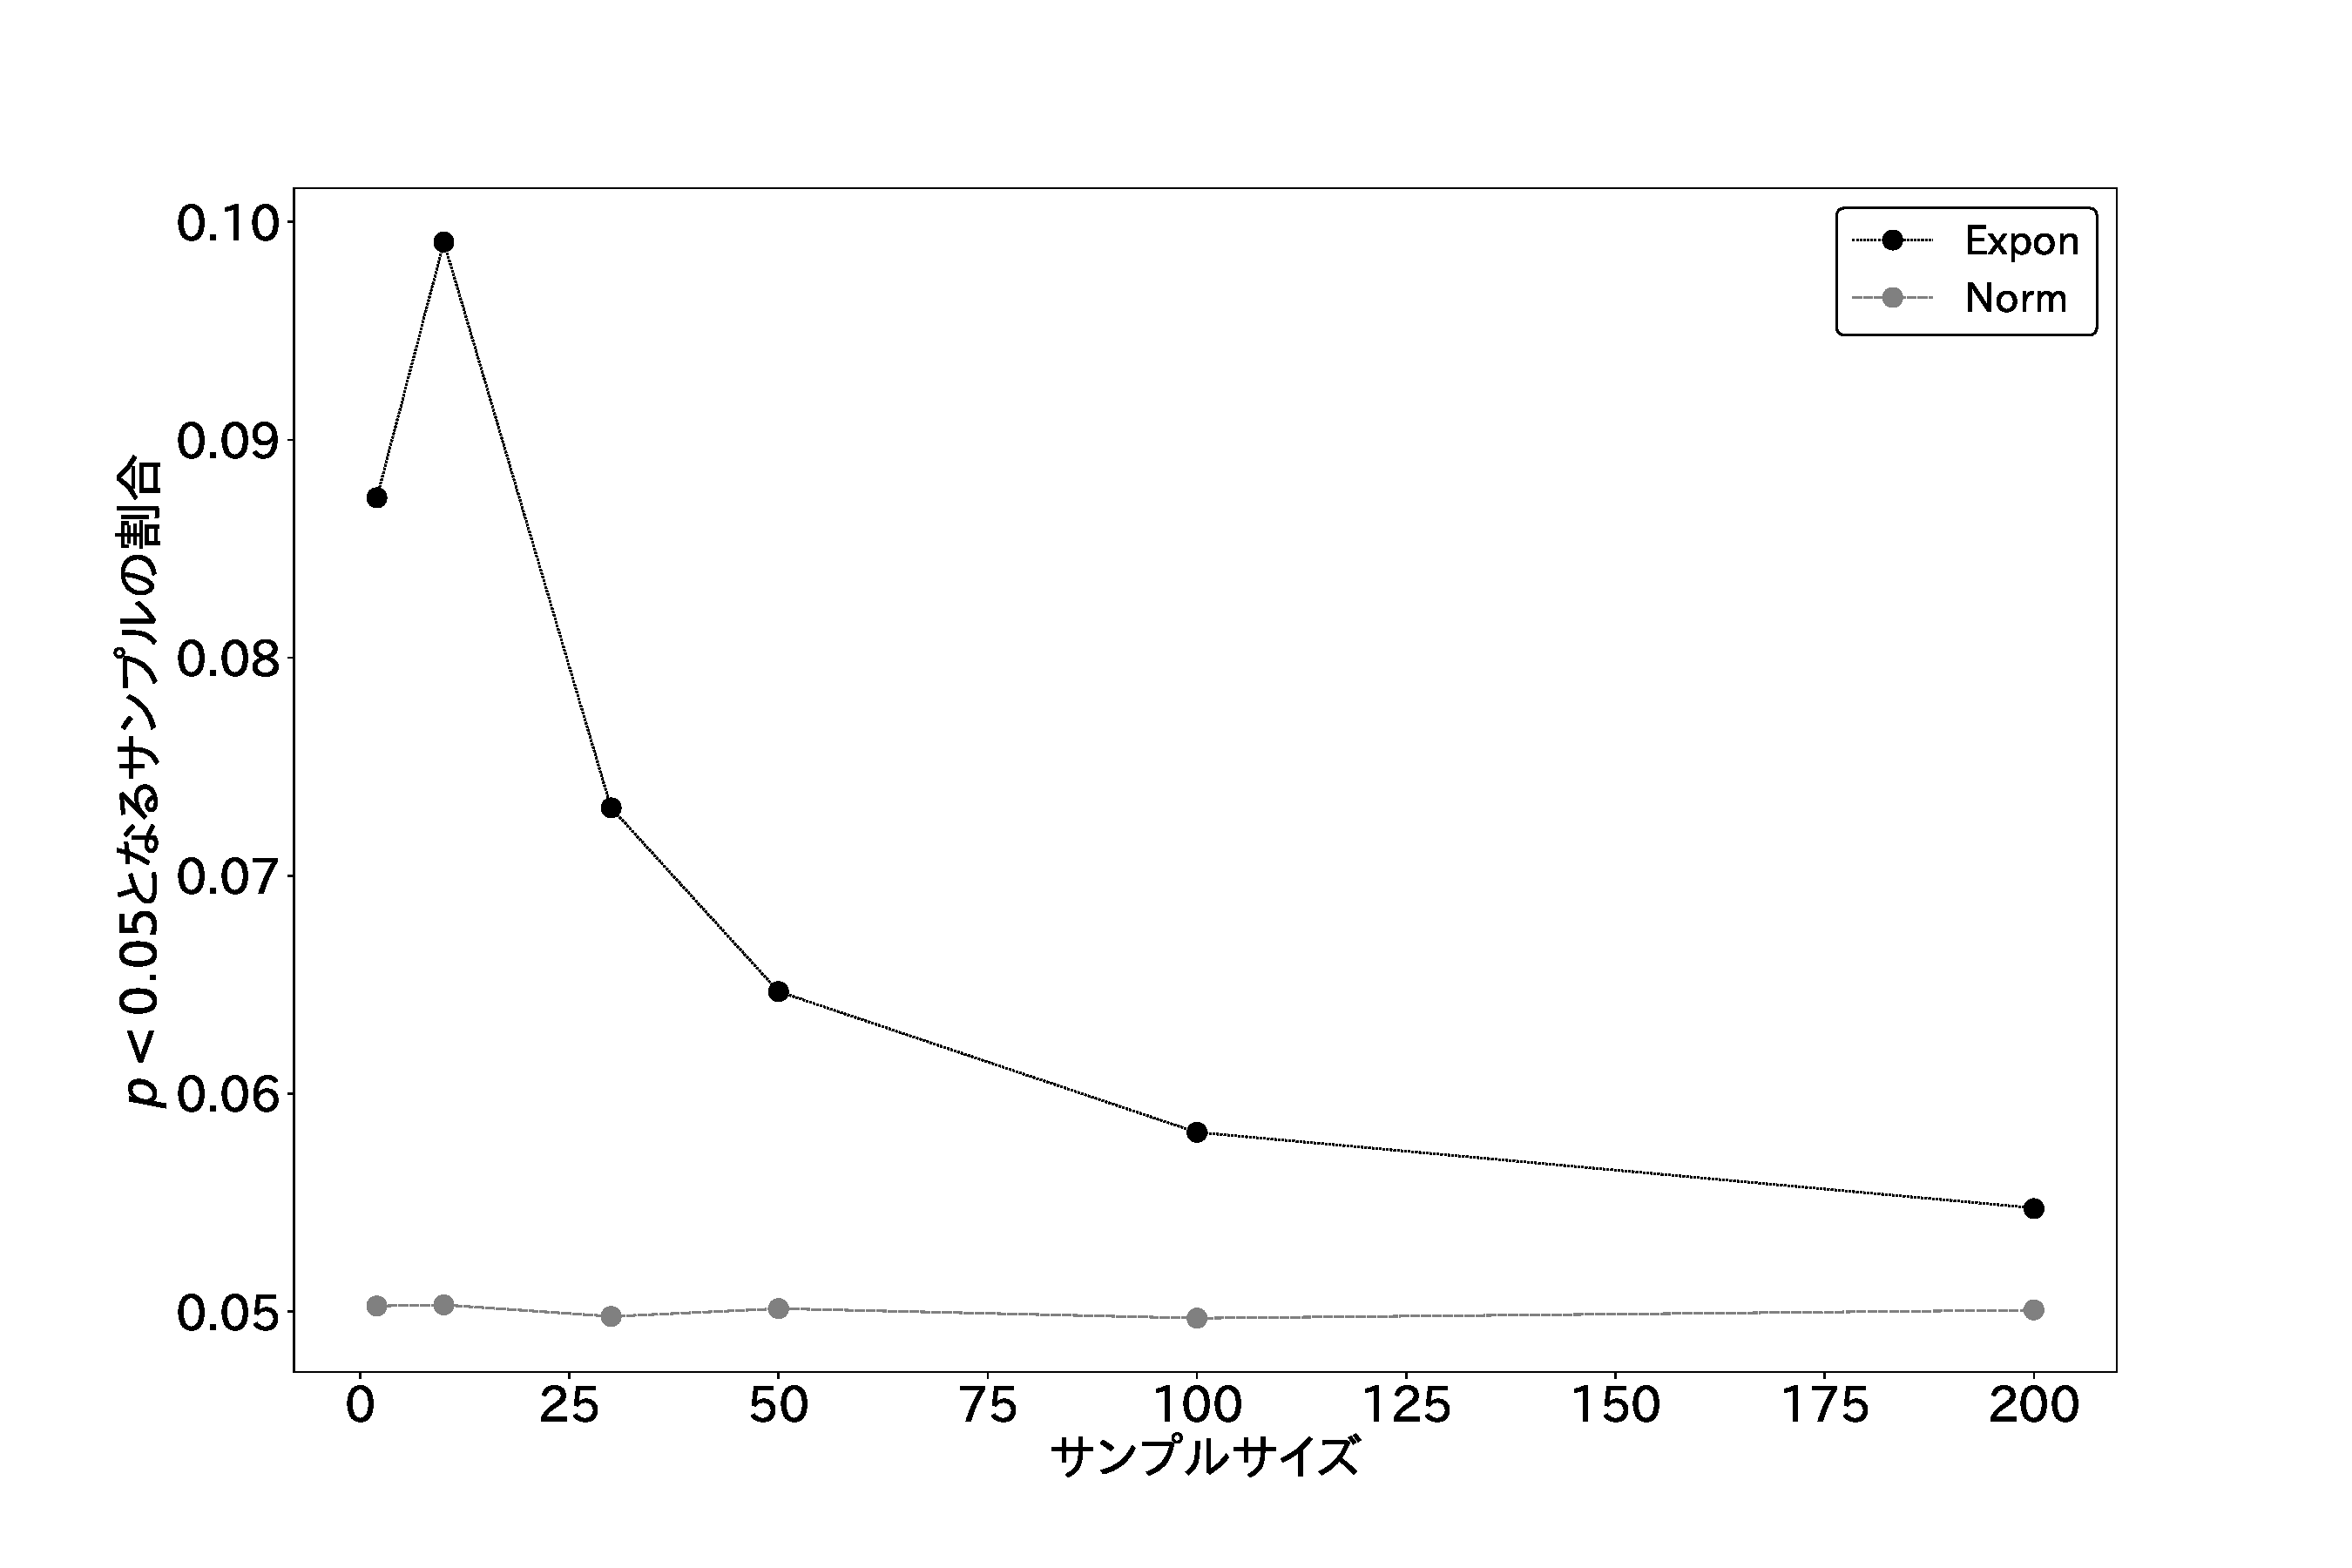
\includegraphics[width=15cm]{./image/04_/t_test_expon_norm.pdf}
        \caption{正規分布または指数ぶんぷから得た標本の$T$値から計算した$p$値で、$p<0.05$以下になる割合}
    \end{center}
\end{figure}

シミュレーションの結果、正規分布から標本を得た場合、$p<0.05$になる割合は、サンプルサイズに依存せず、$5\%$程度であり、期待通りである。
一方で、指数分布から標本を得た場合、$p<0.05$になる割合はサンプルサイズに応じて変化しており、また、どのサンプルサイズでも$p<0.05$となる割合は$5\%$より多い。

このことから、指数モデルの$\alpha_1$は、$\alpha_1>0.05$であることがわかり、統計量を正しく選ばなかったことで、自己否定の過誤が期待した$0.05$よりも大きくなっていることがわかる。

\if 0 
これはいらない
\begin{SMbox}{サンプルサイズがxx以上あるから$t$検定}
        サンプルサイズがある値以上あるので、中心極限定理により、$t$検定が利用できるというものもある\footnote{http://id.ndl.go.jp/bib/024660739}。このロジックが読み込めなかったので、その謎を明らかにすべく我々はアマゾンの奥地へ向かった。

        %サンプルサイズが1以上であれば、$t$検定を行うことは原理的には可能である。
        データが指数分布的であるときに、$t$検定を使うときに生じる問題は上でみた通りであり、$p<0.05$となる標本の割合が多くなっているので、間違った推測をする可能性が高くなる。
        他の分布関数でもおそらく同じような現象が現れる。
        このことから、我々は「$t$検定が利用可能である」は正確ではなく、「$t$検定を使うことができるが、間違った推測である確率が高くなる」ということだと推察した。

        %サンプルサイズが大きくなれば、$\alpha_1$は小さくなる。
        業界によっては、サンプルサイズが$xx$以上であれば、過誤を無視して良いというふうに言われることもある。実際には、設計したモデルと
\end{SMbox}
\fi

\subsection{検定を繰り返し使おう($\alpha_2$)}
ここまでは、一つの標本に対して、統計モデル$M(\mu)$により推測できるかを考えていた。
ここでは、$\sigma^2=10^2$とした正規モデル$M(\mu)$によって複数の標本について推測できるかを仮説検定を指標にし考える。
%ここでは、複数の標本について、$M(\mu)$により推測できるかを
標本が$3$個あるとする。このとき、それぞれの標本の統計量$T$が信頼区間に入っている確率は、$(1-\alpha)$である。全ての標本の統計量$T$が信頼区間に入っている確率は、その積$(1-\alpha)\times(1-\alpha)\times(1-\alpha)=(1-\alpha)^3$であり、この確率で統計モデルは棄却されない。
一方で、棄却される確率は、$1-(1-\alpha)^3$である。
\begin{table}[hbtp]
    \caption{標本数に応じた$\alpha_2$}
    \label{table:multiple_test_reject_prob}
    \centering
    \begin{tabular}{lcr}
      \hline
      標本数  & $\alpha=0.05$  &  $\alpha=0.01$ \\
      \hline \hline
       1 & $0.05$  & $0.01$ \\
       2 & $0.0975$ & $0.0199$\\
       3 & $0.142$ & $0.0297$\\
       4 & $0.185$ & $0.0394$\\
    \end{tabular}
  \end{table}
表\ref{table:multiple_test_reject_prob}は、標本数に応じた$\alpha_2$である。標本数が大きくなるについれて、$\alpha_2$が大きくなることがわかる。

$\alpha_1$がレベル$\alpha$の検定になっていない場合、$\alpha_2$はさらに有意水準$\alpha$から隔たりの多い数値になる。




\section{類似度の過誤}
統計モデルの間の類似度を検出力といった。
統計モデルに対して、不適切な統計量を与えたとき、検出力を歪める。
これを類似度の過誤といい、その確率を$\beta'$で表す。
直接またはシミュレーションを行い$\beta$を計算することがおそらくできそうだが、面倒なので行わない。



\section{データとモデルの比較}
ここで、いくつかのことを定義しておく。
\begin{defi}
    統計モデルと標本を比較して、モデルが母集団のことを予測できないとさまざまな指標をもとに判断するとき、統計モデルを却下すると宣言する。
    %ある標本から求められた統計量以上に大きな値が得られる確率を$p$値と呼ぶ。
    %絶対にダメと判断されないときは、統計モデルを採択(棄却の対義語)すると宣言しない。
    %統計モデルが棄却されるのは、統計モデルの仮定によって変化する。本書の範囲内であれば、統計モデルの母数、分布関数、独立同一の分布関数からサンプリングされたことによる。
    %最尤統計モデルにおいて、棄却されない統計モデルの母数の範囲を信頼区間といい、棄却されるモデルの母数の範囲を棄却域という。
\end{defi}
%ある閾値$\alpha$を決めて、それよりも小さな$p$値をもつ標本について、モデルから得られたものではないと判断する。ここで、$\alpha$を有意水準という。

\begin{SMbox}{検定統計量や$p$を計算するだけで解析完了}
    統計検定量があるモデルに適合的かを示す指標を計算するだけになってしまう。
\end{SMbox}


ここで、母集団から無作為抽出した標本(モデルから生成された標本ではない)を正規モデルにより、予測できるかを考える。
上記の議論と同様に、標本から、統計モデルにあった統計量を計算し、統計量よりも偏った値が出現する確率($p$値)を計算する。
$p$値が小さければ、モデルにより予測できないと考え、値が1に近いほど、もしかしたらモデルで予測できるのかもしれないと考える\footnote{$p$値だけで判断してはいけない}。
標本を元に、モデルにより予測ができないかを考えている。
%このとき、モデルを却下すると宣言する。
%$p$値が$\alpha$よりも小さいとき、流石にこのモデルでは予測できないでしょうと判定する。
%$p$値が$\alpha$よりも大きい場合でも、そのままこのモデルで予測できるとは宣言しない。他の指標やデータとモデルをグラフにより比較し、予測できそうかを考察する必要がある。

%この標本は、モデルからサンプリングしたものではない。
%標本の統計量が、モデルの上で得られやすいものかを調べる。
%$M_a$を棄却する判断をする閾値は、言い換えると、統計モデル$M_a$の棄却される母数(棄却域$R$)の出現確率を$\alpha$とした。


以上のことは、托卵行動に例えることができる。
モズは、カッコウに対して卵を託す托卵を行い、カッコウは、モズの卵とは気が付かず、そのまま育てる。
ここで言い換えたいのは、カッコウは統計モデルであり、卵は標本そして、モズは科学者である。
統計モデルは、モデルからのサンプリングされた標本を巣穴に置いている。
卵の情報を要約した統計量が、モデル由来であることをモデルはその統計量の出現頻度を推測できる。
出現頻度が$p$値である。
モデルの巣に自然から無作為抽出した標本を科学者が置く。
その標本の統計量の出現頻度をモデルは推測できる。
得られた推測から、標本がモデルの卵であることを判定するのは科学者である。
この手順だけでは科学者はモデル鳥と標本卵を比較しているだけであり、標本卵を構成しているデータそのものとモデル鳥を比較していないということに注意しなければならない。


\begin{figure}
    \begin{center}
        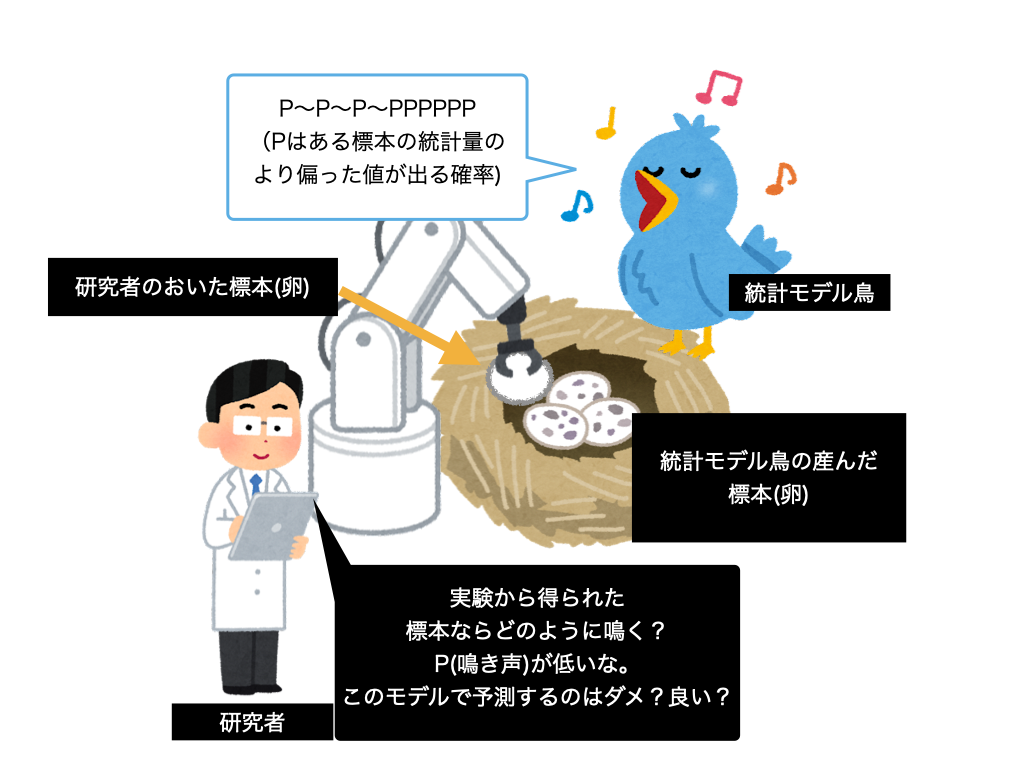
\includegraphics[width=15cm]{./image/01_/conceptual_diagram/conceptual_diagram.003.png}
        \caption{統計量を使ったモデルとデータの比較に関する概念図}
        \label{fig:conceptual_diagram_test}
    \end{center}
\end{figure}
    


\begin{SMbox}{偶然の差が生じたかを確かめたい}
    「偶然の差が生じたかを確かめたい」や「こんなことが起こる確率は$5\%$くらい」という言葉を統計学の教科書で見たことがある。これらは、本書での説明とは異なる前提をもとに議論を進めており、本書と解釈の互換性はない。
    %「統計モデルの上で統計量が現れる確率が十分小さいことを確かめたい」や「統計モデル上でそのような統計量が得られる確率が$5\%$」を省略して書いたものです。
    
    科学では、実験で得られたデータは、同様の実験を行った場合、同様のものが得られるということが前提になっている。このことを現象に再現性があると言う。
    再現性のないデータを現状の統計学で扱うことや、現実の現象が得られる確率を議論することは困難である。

    本書の前提を元にすれば、「こんなこと(これ以上に偏った統計量値)が(モデル内で)起こる確率は$5\%$くらい」ということを省略して「こんなことが起こる確率は$5\%$くらい」と言うことはできる。また、現実において起こりやすいのかどうかについては議論できない。
\end{SMbox}


\subsection{$p$値を使った判断に関する注意}
$p$値を元に統計モデルとデータの不一致を考えるとき、$p$値はモデルとデータの乖離を示す指標の一つであると言うことを意識しなければならない。このことを忘れてしまい、次の間違った判断を行うことがある。
\begin{enumerate}
    \item $p$値が0に近いならば、統計モデルによりデータを予測できないと判断する
    \item $p$値が1に近いならば、統計モデルによりデータを予測できると判断する
\end{enumerate}
それぞれのデータがどのようなものなかのかを確認してみる。
\subsubsection{$p$値が0に近い$\rightarrow$統計モデルによりデータを予測できないと判断}

\subsubsection{$p$値が1に近い$\rightarrow$統計モデルによりデータを予測できると判断}




\begin{SMbox}{P値が小さければ、モデルの仮定のうち少なくとも一つが間違い}
    \ 
    \begin{quote}
        P値が小さければ、データと帰無仮説の矛盾している程度が大きいので、P値が小さければ帰無仮説は棄却するんだと統計の教科書には書かれています。実はそうではなくって、今お話ししたように小さいP値が何を意味するかというと、たくさんある統計モデルの仮定のうちどれか一つが間違っているあるいは、複数のものが間違っている。決して帰無仮説だけが間違いの対象ではなくって、先程のように、小さいP値が選択的に報告してあれば、結果としては誤った結果になります。・・・・
        %ランダム化もランダムサンプリングもなされていなければ、そもそも、データに対して確率計算をすることも意味がないことですから、そういうデータでなければ、P値を計算する意味すらなくなってしまう。
        \footnote{京都大学大学院医学研究科 聴講コース 臨床研究者のための生物統計学「仮説検定とP値の誤解」佐藤 俊哉 医学研究科教授 \url{https://www.youtube.com/watch?v=vz9cZnB1d1c} }
    \end{quote}
    P値が小さければ、モデルの仮定のうち少なくとも一つが誤っているというものがある。私はこの意見に賛成できない。

    モデルの中で標本の統計量以上の値の出現確率を計算したものが$P$値である。$P$値によって、仮定の間違いを主張できるような値ではない。ある母数を持つモデルによりデータの平均値を予測できなかったことを示唆すのが$P$値である(パラメトリックモデルの範囲であれば)。
    正規分布や独立同分布ではないことを示唆することはおそらくない。

    ただ、モデルとデータの比較を行なった後、データが目的にあっているのかを調べなければならない。
    %モデルの仮定をデータが満たしていることを$P$値では測れない。モデルの仮定をデータが満たすことはほとんどない。
\end{SMbox}


\begin{SMbox}{モデルの仮定を満たせるのか}
    \ 
    \begin{quote}
    最初の原則。最初に述べられている原則ですが、P値はデータと特定の統計モデルが矛盾する程度を示す指標の一つであるというふうに書かれています。ここでですね、統計モデルは何かって言うと、統計モデルは必ず一連の仮定のもとで構成されています。どんな仮定かと言いますと、統計の教科書をみますと、「データが正規分布している」とか、「平均値が等しい」などが統計モデルに必要な仮定とされているのですが、まず、一番大切なことは、データを撮るときに、先程の試験のように、薬剤のランダム割り当てが行われているとか、対象者を剪定するときにランダムサンプリングがなされているか、こういったことも統計モデルの仮定に含まれています。
    それから当然、研究計画がきちんと守られているかも統計モデルが必要とする前提の一つです。例えば、先程の臨床試験で言えば、
    結果の解釈も変わってきます。最後まで対象者が追跡できているのか。追跡不能とからつだくがあったとすると、統計モデルの後世に影響を与えます。もちろん解析方法も妥当な結果を与える解析方法でなければいけない。
    こういったことを満たしていなければ、統計モデルの仮定を満たしているとは言えない。
    %もちろん、全ての解析結果が報告されている。これは統計モデルに必要な仮定とは言えないですが・・・
    \footnote{京都大学大学院医学研究科 聴講コース 臨床研究者のための生物統計学「仮説検定とP値の誤解」佐藤 俊哉 医学研究科教授 \url{https://www.youtube.com/watch?v=vz9cZnB1d1c} }
    \end{quote}

    この意見は統計モデルに関する仮定と実験計画の二つの要素が混じっている。実験計画を統計モデルの仮定を満たすように設計するという意見だと考えられる。
    この意見に賛成しない。

     まず、統計モデルの仮定が自然において対応するものが、本書においてはない。また、「平均値が等しい」という仮定であるが、ある平均値をもつ統計モデルとデータを比べるさいに、データの平均値が異なる場合においても、統計モデルを使ってそのデータの出現頻度などを推定することが可能である。
     このことは、モデルの仮定をデータが満たさなければならないことを示唆していない。

     次に、実験計画については、科学者がみたい効果を見るために設定しているのもである。ランダムサンプリングしているのは、対象に偏りがないようにし、さまざまな対象である特徴の変化を与え、その集団内での変化を計測するために行う。
     対象の選定に偏りがあった場合、本当に推測したかったことが推測できない。例えば、成人以上を対象にした試験なのに、60歳だけしかからサンプリングできなかったなら、成人に対しての言及はできない。
     また、偏りのあるデータを偏りを前提としていない統計モデルにより解釈するのはこんなんである。
     この困難さを回避するためにも実験デザインを守った無作為抽出であった方が良い。
     
     いずれも本書の方針とは異なる。
     %モデルに対してではなく、科学者がみたいものが見れなくなることを意味する。
     %モデルは偏ったデータが得られたことを考慮して構築していない。
     %モデル自体に偏りを設定すればよいはずであるが、


     %医学における研究が予測精度を高めるということを目的にして統計学を使っていないので、意見が一致しない。
\end{SMbox}

%%%
\section{モデルと標本の乖離による過誤}
データとモデルを統計量により比較したとき、その乖離について測ることのできないことをまとめる。

\subsection{モデルの確率密度関数と標本の分布の乖離による過誤}
経験がないことで、適当なモデルを構築し、非常に少数のサンプルサイズしか得られないことで、そのモデルの妥当性について検証できないまま、モデルとデータを仮説検定により比較し、判断することにより生じる間違いである。
例えば、データの分布が非対称に分布しているのに、正規分布を含んだ統計モデルを構築し、$T$統計量により検定をおこなったとする\footnote{データが非対称に分布していることから、正規分布を含んだ統計モデルでは推論できないことがわかるので、統計検定を使う意義はなくなると思う}。前の節でみたように、分布関数に対して適切な統計量を選ばなければ$\alpha_1$が設定した有意水準$\alpha$とならないので、期待していた推論が行えないことが多くなる。

\subsection{無作為抽出されていない事による過誤}
対象を無作為に抽出できていない標本から、統計量を計算し、モデルの母数を推定したとする。
このモデルでは、本来設定した母集団に関する予測には誤りが多くなる。
例えば、17歳の日本人男性の身長を母集団に指定したのに、17歳のバスケ部部員の身長を計測すると、その標本はひどく偏ったものになる。
その標本を元に、モデルの母数を推定し、母集団に関する推測を行う。
すると、間違った推測が得られる。例えば、平均が大きくなりすぎたりすることが予想される。


\subsubsection{後付けの母集団かつ$p<\alpha$を満たす集団}
$p<\alpha$であるという標本がデータから発見されたので、標本の特性を持つと思われる母集団を後付けし、その母集団から無作為抽出を行なったことにし、統計モデルが棄却されたというストーリーを作ったとする。
言い換えれば、後付けの母集団ならば、$p<\alpha$であるという論理を構築したことになる。
実際には、後付けの母集団でありかつ$p<\alpha$という集団から作為抽出しているので\footnote{この場合でも無作為抽出できていると誤解してしまうが、後付けの母集団から無作為抽出できていない!}、本来の母集団については何もわからない。言い換えれば、母集団に関する拡大解釈が行われたことで、母集団に関しては何もわからないのに、推測を行なったと間違えた主張をしている\footnote{母集団デカすぎの過誤である}。
母集団の特徴を知るには、無作為抽出を行い、推測を行う必要がある。

このような母集団に関する拡大解釈を仮説ハッキング($HARKing$)といい、この操作により得たデータと仮説について、仮説が元からあったことにして、報告を行うと、研究不正となる\footnote{
    HARKingは、再現性の問題という意見もある。
    \url{https://twitter.com/ykamit/status/1077716200845500416} 。この意見に私は同意する。私は、母集団を無作為抽出していないことで、再現できないことが増えると考えている。
}
\footnote{
    多重検定により、$p$値が低く推測されることが問題であるというものもある\cite{池田_功毅2016,中村_大輝2021sp20016}。部分的には同意できるが、私は十分理解できなかった。
}\footnote{
    Twitterでのアンケートでは、多くの人がHARkingをうまく理解できてないというTwitterでのアンケートもある。
    \url{https://twitter.com/biomedcircus/status/1088957697368690689}
}\footnote{
    探索的なデータ解析においては、帰無仮説の後付けが許されるという主張もある。この意見には同意できない。母集団について拡大解釈をすることは許されない。探索的データ解析により得られるのは、母集団かつ$p<\alpha$という集団が見つかったということのみ主張でき、母集団についての推測をしたと主張はしない方が良い。
}\footnote{
    HARKingについては、\cite{kerr1998harking}に詳しくまとめられている
}。


\subsubsection{$p<\alpha$になったら無作為抽出を終える}
$p$値がある値を下回ったときに、実験を終了するという操作を行なったとする。
統計モデルの予測と一致するように、母集団を選択したことになる。
この場合、無作為抽出した集団により、設定した母集団に関する性質を調べるという研究目的を達成できない。
「母集団かつ設定したモデルにおいて$p<\alpha$である」集団に関する調査を行なっていることになる。

調査を終えて、この標本についてモデルを使った予測ができないと主張できない。
この不正な操作をアステリスクシーキングという。

\if 0
\subsection{標本の分布がわからない事による過誤}
TODO: よくわからない。
以上により仮説検定は、既知の母集団と変異を与えた母集団との違いを図る方法の一つの方法であると言える。
母集団分布が既知でないならば統計モデルをかんで構築する必要があり、そこから変異を捉えることを試みると、
モデルの仮定と標本の特徴が一致しないことにより、過誤が生じる。

\subsubsection{独立同分布ではない事による過誤}
モデルでは、確率変数は独立であるが、自然現象の多くはなんらかの相関を持っていることが多い。
人間の身長であっても、同じ社会の中にいれば、各個人がなんからの相関を持つとも考えられる。
そんなことは、おいておいて、それぞれ独立だと思って解析してみると言うのが統計学を使った方法であるので、
自然とモデルの間にはやはりギャップが存在し、モデルの想定よりもあらい推定になることがあり得る。
\fi
\if 0
\paragraph{$p<0.05$にした理由}
https://biolab.sakura.ne.jp/statistics-5-percent.html
\fi



\if 0
\subsection{サンプルサイズが小さければ$t$検定}
西内啓 著「統計学が最強の学問である(実践編)」(ダイヤモンド社)
\url{https://biolab.sakura.ne.jp/small-sample-t-test-glm.html}
\fi 

\chapter{尤度比を使ったモデルとデータの比較}
モデル$M$において得られるデータ元に、母数を最尤推定する。新たに作られた最尤モデル上での尤度と元のモデル$M$での尤度の比がある分布に従うことがわかっている。
このことを利用して、もともモデル$M$でデータを予測してもいいのかを考察する。

前の章で統計検定をモデル鳥によって説明した。あるモデル鳥が生んだ標本卵に関する統計量のばらつきの特徴と、研究者が持ってきたデータ卵を比較し、そのモデル鳥が産んだと判定していいのかを考える方法と説明した。
ここでも、どのモデルが生んだ標本卵に関わる予測なのかを考えなくてはならない。
あるフルモデルにおける予想分布をまずは考察する。

\section{概要}

\begin{defi}
    母数の数が異なる統計モデル間の尤度の比を次のように定義する。
    \begin{equation*}
        Dev(D,M_1,M_2) = -2\log\frac{M_1におけるDの尤度}{M_2におけるDの尤度}
    \end{equation*}
    ここで、$M_1$は、$M(\theta_1,\theta_2)$,$M_2$は$M((\theta_{1'},\theta_2))$であり、$\theta_1$と$\theta_2$のベクトルの要素数の和は、$\theta_{1'},\theta_2$のベクトルの要素数の和に等しい。$D$は標本とする。

\end{defi}

$M_1$における標本$D$から、最尤モデル$M_1(\hat{\theta_1})$を構築したとき、$Dev(D,M_1,M_1(\hat{\theta_1}))$は、
\begin{equation*}
    Dev(D,M_1,M_1(\hat{\theta_1})) \sim \chi^2_{p}
\end{equation*}
であることがわかる。ここで、$p$は、$\theta_1$の要素数。
例えば、正規モデル$M(170,5.8^2)$から標本$D$を生成する。その$\mu$に対する最尤モデル$M(\hat{\mu})$は、次のようになる。
\begin{equation*}
    Dev(D,M(170,5.8),M(\hat{\mu})) \sim \chi^2_1
\end{equation*}
データ由来の母数の個数が$1$なので、自由度$1$の$\chi^2$分布に従う。

あるデータ$D'$に対して、最尤推定を行なったモデル$\hat{M}$について、次のことがわかる。
\begin{equation*}
    Dev(D,\hat{M},\hat{\hat{M}}) = -2\log\frac{\hat{M}におけるDの尤度}{\hat{\hat{M}}におけるDの尤度} \sim \chi^2_{p}
\end{equation*}
ここで$D$は、$\hat{M}$の標本であり、$\hat{\hat{M}}$は、標本$D$を使って$\hat{M}$のいくつかの母数の最尤推定を行なったモデル、$p$は$\hat{\hat{M}}$において最尤推定を行なった母数の個数。

\subsection{データと当てはめモデル$\hat{M}$の比較}
データ$D$を当てはめていないモデル$M$に対して、$D$を予測できるかを確かめる。
パラメータの個数が少ないモデル$M'$についての尤度比は次で計算できる。
\begin{equation*}
    Dev(D,M,M')
\end{equation*}
$M$によって、$D$について十分な予測ができるならば、パラメータを任意の個数減らしたモデル$M'$との尤度比は、$Dev(D,M,M')$が自由度は元のパラメータ数-自由度+1となる$\chi^2$分布に従う。
このことから、$Dev(D,M,M')$が比較的小さな値であれば($p$値は比較的大きくなっている)、モデル$M$によって予測可能であることの根拠の一つになりうる。


\subsection{データと当てはめモデル$\hat{M}$の比較}
当てはめたモデル$\hat{M}$とデータの比較。
次を計算する。$D'$を観測データとする。
\begin{equation*}
    Dev(D',\hat{M},\hat{\hat{M}}) 
\end{equation*}
ここで、$M$の標本$D'$の最尤推定モデルを$\hat{M}$とし、$\hat{\hat{M}}$は$\hat{M}$の$p$個の母数に対して最尤推定を行なったモデルである。
$Dev(D,\hat{M},\hat{\hat{M}}) $の分布($\chi^2_p$)の中で、$Dev(D',\hat{M},\hat{\hat{M}}) $が珍しい値を取っていたなら、
$\hat{M}$から考えられる尤度比の変動の中では、比較的大きな変動が起きていることが示唆される。
このことから、$\hat{M}$で標本を予想しない方が良いのではないだろうかと判断する。

注意しなければいけないのは、$\hat{\hat{M}}$の方が良いとは言えてないことである。
当てはまりの良さは、尤度の大小関係を見れば良い\footnote{次は何かがおかしい「尤度の大小関係が有意であることを確かめるのが尤度比検定である。」。}。%有意かどうかとはどういう意味かがわからない。$\hat{M}$の尤度比の変動では予測できないという意味であれば理解できる。さまざまな前提で検定が使われているので、解釈が一致しない。}。

\if 0
この性質を利用して、母数の数の異なるモデルに対して、最尤推定をそれぞれ行い、モデルを構成する。
ある統計モデル$M_1$とし、$M_1$の中でいくつかの母数を固定したモデル$M_2$とする。
$M_1$からサンプリングした標本とその最尤モデル$M_{1'}$は尤度の比が$\chi^2$に従う。
同様に、その標本に対する最優モデル$M_{2'}$とすれば、$M_1$と$M_{2'}$の尤度比も$\chi^2$分布に従う。

ここで、母集団から無作為抽出した標本$D$とする。
$D$の最尤モデルを$M_{1''}$、$M_{2''}$とする。
これらモデル上での尤度の比を計算し、$\chi^2$においてどの程度の珍しさなのかを調べる。


そのモデルでのならば、どの程度の珍しさなのかを計算する。
尤度比が大きくなれば、$\chi^2$において珍しい値になり、$p$値が小さくなる。
言い換えれば、あるモデルで予想される尤度の比と比べて、データから導かれた尤度比が大きな変動かが計算できる。
\fi

\begin{SMbox}{尤度比検定で$p<0.05$だったので$M_1$より$M_2$がより適合的だ}
    尤度比検定で$p<0.05$だったので$M_1$より$M_2$がより適合的だという判断はしないほうが良い。
    尤度比検定において$p$値が小さいということは、
    $M_1$における尤度比の予測値の中で、比較的大きな尤度の変化が実験データでは生じていることを示したことになる。
    これは、$M_1$の中での変動と比較しているだけである。
    相対的に$M_2$の方がより適合的であることを示唆していない。
    
    より適合的であることを示す量は、尤度である。
    対数尤度が小さい方がデータに対して適合しているという判断ができる。
\end{SMbox}



\if 0
\paragraph{尤度比}
データを指数分布から生成し、モデルを正規モデル$M$とする。
二つの母数についての最尤モデルと、平均
このとき、何度もデータを指数分布から生成し、尤度比を計算したとき、その尤度比は$\chi^2$に従うか?
%無作為抽出して得た標本に対して、あるモデルのその標本に対する最尤モデルを$M(\theta_1,\theta_2,\theta_3)$とする。
\fi

\section{尤度比検定}
母数の個数が$k$個のモデル$M(\theta)$とする($\theta$は$k$次元ベクトル)。
モデル$M(\theta)$からサンプリングしたサンプルサイズ$n$の標本$x=(x_1,x_2,\cdots,x_n)$を得たとする。
この標本$X$から$\theta$のうち$r$個の母数に関する最尤推定量を$\bar{\theta}$得たとする。
$\bar{\theta}$のうち$k-r$個はモデル由来の母数であり、$r$個は標本から推定した母数である。
このことから、$\bar{\theta}$は自由度$r$の母数のベクトルと言う。

もとのモデル$M(\theta)$における標本$X$に対する尤度は、$L(\theta,x)$とする。
また、最尤モデル$M(\bar{\theta})$での尤度は、$L(\bar{\theta},x)$とする。
このとき、これら尤度の比がカイ二乗分布分布に従うことがわかっている\footnote{ただしいくらかの条件がある}。
つまり、
\begin{equation*}
    -2\log\lambda(X)\sim \chi^2_{k-r}
\end{equation*}
ただし、
\begin{equation*}
    \lambda(X) = \frac{L(\theta,x)}{L(\bar{\theta},x)} 
\end{equation*}
である。


\begin{SMbox}{滅多に観察されない逸脱度}
\begin{quote}
    有意確率が小さければ(通常は$5\%$以下)\footnote{おそらく$p$値が小さければ}、2つのモデルの「逸脱度の差」は滅多に観察されないほど大きな値であると判断する。
\end{quote}
    これは本書とは異なる方針の科学における指針である\footnote{
        この話は後でもう一度考えて見た方がいい気がする。
        できないはずであるが、できるとする論文が多い。なぜなんだろうTODO。
    }。

    本書では、ある統計モデルが予測した統計量と比較して大きな統計量が得られたからといって、現実的に滅多に観察されないとは解釈しない。

    本書が扱いたい科学において、
    一般化線型モデルを使えば、現実での起こりやすさが検証できるということはおそらくない。
    %https://www.jstage.jst.go.jp/article/weed/55/4/55_4_275/_pdf
    %特集 統計解析(再?)入門 R を用いた一般化線形モデル(仮説検定編): 割合データを例
\begin{quote}
    2つのモデルの「逸脱度の差」が大きいことから、すなわち、要因を覗くことでモデルの当てはまりが十分に悪くなることから、その要因は有意な要因であると判断する。
\end{quote}
    これも本書とは異なる分野を研究しているのだと思われる。

    尤度比の差の統計量を実データの尤度比の差と比べてわかるのは、フルモデルで予測または当てはめしない方が良さそうということである。
    より当てはまりのモデルかどうかは尤度比を比べればよい。
\end{SMbox}

\section{正規モデルにおける尤度比検定}

$\sigma^2_0$を設定した正規モデル$M(\mu_0;\sigma^2_0)$について考察する。
この正規モデルからサンプリングを行なった標本$X$とする。
標本から得た最尤正規モデルを$M(\bar{x};\sigma^2_0)$とする。
それぞれのモデル内での標本$X$の尤度を$L(\mu_0,X),L(\bar{x},X)$とする。
具体的な数式は、
\begin{align}
    L(\mu_0,X)=\frac{1}{\sqrt{2\pi\sigma^2}}\exp(-\frac{\sum(x_i-\mu_0)}{2\sigma^2})\\
    L(\bar{X},X)=\frac{1}{\sqrt{2\pi\sigma^2}}\exp(-\frac{\sum(x_i-\bar{X})}{2\sigma^2})\\
\end{align}
これらから$\lambda(X)$を計算すると、
\begin{align}
    -2\log\lambda(X) &= -2(-\frac{n}{2\sigma^2_0}(\bar{x}-\mu_0)^2) \\
    &= \frac{n}{\sigma^2_0}(\bar{x}-\mu_0)^2 \sim \chi^2_1 \\
\end{align}
である。

\subsubsection{数値実験}
モデルと同じ確率密度関数からサンプリングを行い、尤度比検定を行なってみる。

数値実験を行なってみる。具体的に、正規分布$N(170,5.8^2)$からサンプリングした標本1000個を集める。
標本から平均値を求め、これを最尤推定量とする(xbar)。
この最尤モデル$M(\mu;\sigma^2=5.8^2) $における標本の尤度を計算する(loglike2)。
同様に、モデル$M(170;\sigma^2=5.8^2)$における標本の尤度を計算する(loglike)。
以上から尤度比を計算し、それが$\chi^2_1$分布と一致することを確かめる。
以下がコードである。

\begin{lstlisting}
norm_ = norm(170,5.8)
data_ = norm.rvs(170,5.8,size=(1000,10))
xbar = np.average(data_,axis=1)
loglike_ = np.prod(norm_.pdf(data_),axis=1)
#loglike2_ = np.prod(norm(xbar,5.8).pdf(data_),axis=0)
#print(np.prod(norm(xbar,5.8).pdf(data_),axis=1),xbar)

loglike2_ = []
for item in data_:
    #print(item.shape)
    a = norm(np.average(item),5.8).pdf(item)
    loglike2_.append(np.prod(a))

y = -2*np.log(loglike_/loglike2_)
x = sorted(y)
y_ = np.arange(len(y))/len(x)
plt.plot(x,y_)
plt.plot(x,chi2.cdf(x,df=1))
plt.show()

\end{lstlisting}

$N(170,5.8^2)$と$N(175,5.8^2)$と言う2種類の密度関数からサンプリングを行いそれぞれ結果を図\ref{fig:loglikelihood_test_simulation_norm}(a)および(b)に示す。
図\ref{fig:loglikelihood_test_simulation_norm}(a)は、モデルとデータの分布が一致していることから、累積分布が$\chi^2_1$の累積分布にかなり近いことがわかる。
図\ref{fig:loglikelihood_test_simulation_norm}(b)は、モデルとデータが一致していない状況での結果を示している。尤度比の多くが右に移動しており、標本の多くが$\chi^2_1$において珍しいと判定されやすくなっている。


\begin{figure}
    \begin{center}
        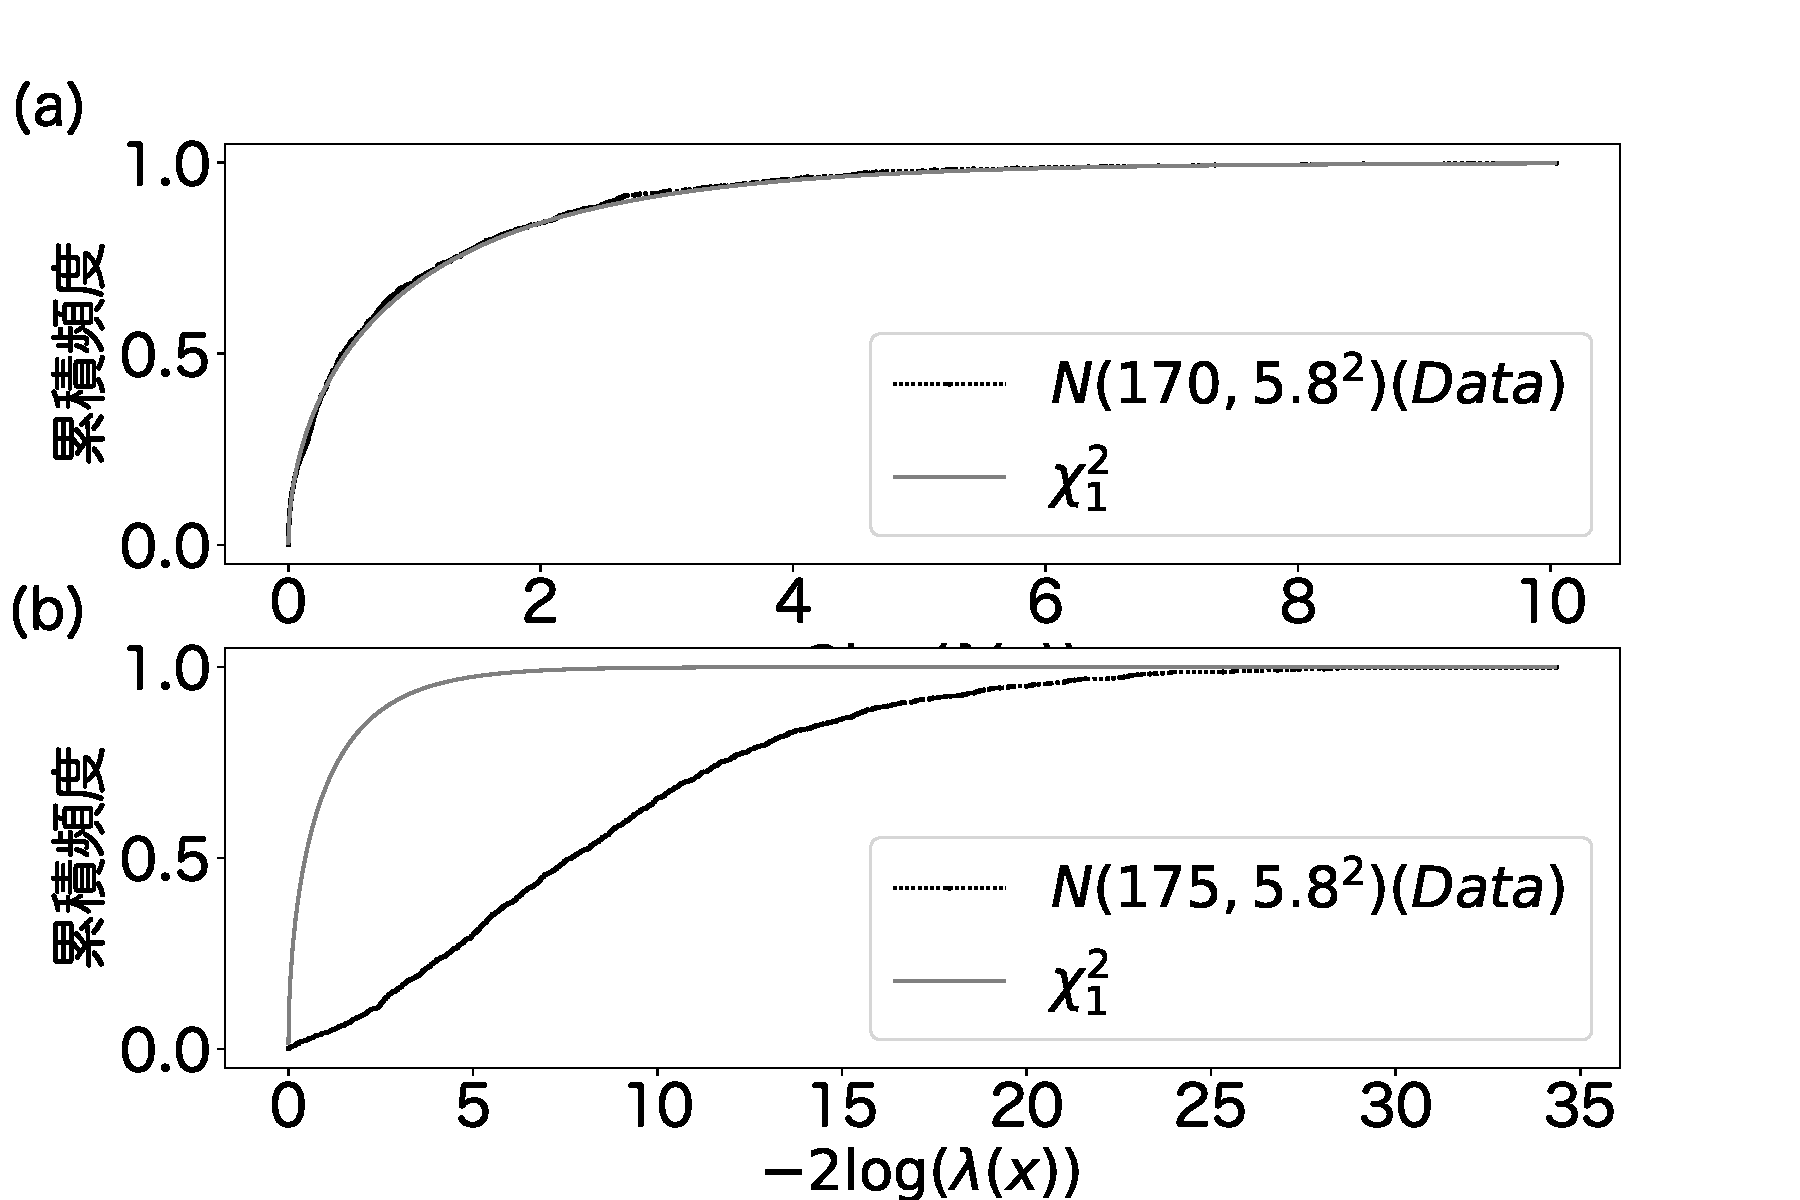
\includegraphics[width=15cm]{./image/04_/loglikeli_norm_test.pdf}
        \caption{対数尤度比の累積頻度。モデルは正規モデル$M(170;\sigma^2=5.8^2)$。(a)標本を$N(170,5.8^2)$からサンプリングした結果。(b)標本を$N(175,5.8^2)$からサンプリングした標本。}
        \label{fig:loglikelihood_test_simulation_norm}

      \end{center}
    \end{figure}

\subsection{データとモデルの乖離を検証する}
モデル上において、その標本を元にした最尤モデルにおける尤度比が$\chi^2_1$に従うことを示した。このことを元に、データをモデルによって予測可能かを調べる。手順は、
\begin{enumerate}
    \item 標本を$x$とする。
    \item モデル$M$における最尤推定量を計算する。
    \item モデル$M$および最尤モデル$M_{MLE}$における標本$x$に対する尤度を計算する
    \item 尤度比および$-2\log\lambda(x)$を計算し、$\chi^2_1$において珍しい値なのかを検証する。
\end{enumerate}
実際に、正規モデルにおいてこの手順をなぞってみる。
$M(\mu;\sigma^2)$における最尤モデルは、$M(\bar{x};\sigma^2)$である。
それぞれのモデルにおける尤度を計算し、$-2\log\lambda{x}$を計算すればよい。

\section{複雑なモデルでの尤度比検定}
次のモデル$M(\beta_1,\beta_2)$を考える。
\begin{enumerate}
    \item $x_i$は定数。
    \item $y_i$は以下に示す分布$p(y_i;\lambda_i)$に従う。
    \item $\lambda_i = \exp(\beta_1+\beta_2 x_i)$
    \item $y_i \sim p(y_i;\lambda_i) = \frac{\lambda_i^{y_i}\exp(-\lambda_i)}{y_i!}$
\end{enumerate}
無作為抽出した標本$x$における2つの最尤モデルを考える。
最初のモデルは、$\beta_2=0$とした上で、$\beta_2$に関する最尤推定を行なったモデル$M_1=M(\hat{\beta_1},\beta_2=0)$である。
このモデルでは、$x_i$に応じて、$\lambda_i$が変化しないので、$\lambda$が常に一定のモデルになる。言い換えれば、$y$が母数$\lambda=\exp(\beta_1)$のポアソン分布となるモデルである。
次のモデルは、$\beta_1,\beta_2$の両方について最尤推定を行なったモデル$M_2=M(\hat{\hat{\beta_1}},\hat{\hat{\beta_2}})$である。
このモデルにおいて、$(x_i,y_i)$はペアになっており、$x_i$に応じて$y_i$が揺らぎを持って決まる。

ここで、$M_1$における尤度比が$\chi_1^2$に従うことを確かめる。手順は以下の通りである。
\begin{enumerate}
    \item $M_1$においてサンプリングを行い、$(x_i,y_i)$からなる標本$X$を得る。$x_i$は、既存の標本$x$のものを使う。$(x_i,y_i)$に関してバラバラになった標本が得られる。
    \item $M_1$における標本$X$の尤度$L_1$を計算する。
    \item $M_2$における標本$X$の尤度$L_2$を計算する。
    \item $-2\log\frac{L_1}{L_2}$を計算する。以上を繰り返す。
\end{enumerate}
以上を行うと、$\chi^2_1$に従うことがわかる。図\ref{fig:loglikelihood_test_simulation_poisson}a,bに結果を載せている。
コードを書いておく。
\begin{lstlisting}
df  = pd.read_csv("https://raw.githubusercontent.com/tushuhei/statisticalDataModeling/master/data3a.csv")

def get_dd(d):
    d['y_rnd'] = np.random.poisson(np.mean(d.y),len(d.y))
    model1 = smf.glm(formula='y_rnd~1',data=d,
    family=sm.families.Poisson())
    model2 = smf.glm(formula = 'y_rnd~x',data=d,family=sm.families.Poisson())
    #print(fit1.summary())
    fit1 = model1.fit()
    fit2 = model2.fit()
    return fit1.deviance - fit2.deviance

l = []
for i in range(1000):
    l.append(get_dd(df))


x = sorted(l)
y = np.arange(len(l))/len(l)
plt.plot(x,y)
plt.plot(x, chi2.cdf(x,df = 1))
plt.show()
\end{lstlisting}


\begin{figure}
    \begin{center}
        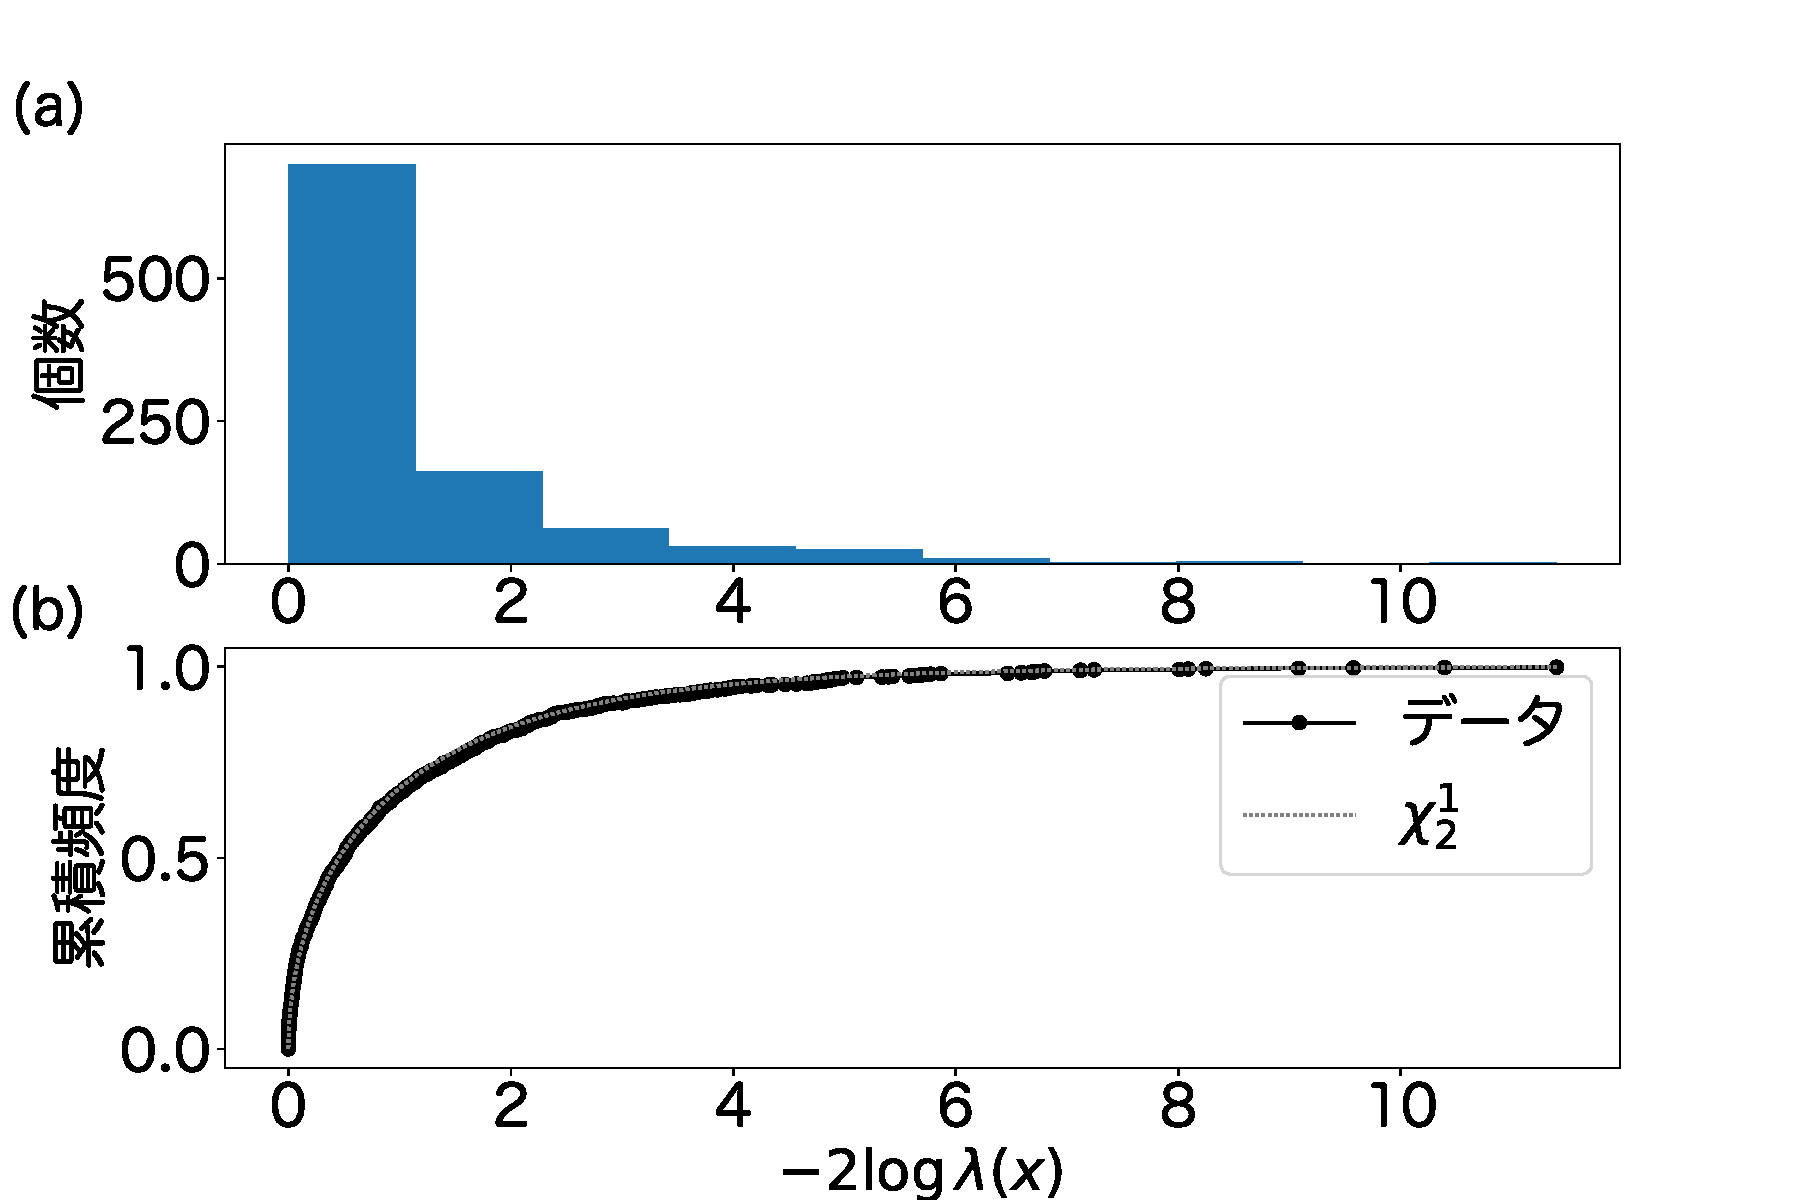
\includegraphics[width=15cm]{./image/04_/loglikeli_poisson_model_test.pdf}
        \caption{$M_1$における対数尤度比の累積頻度。(a)ヒストグラム(b)累積分布}
        \label{fig:loglikelihood_test_simulation_poisson}
    \end{center}
\end{figure}


データと、最尤モデル$M_1$との比較は同様に、
\begin{enumerate}
    \item 標本$x$の尤度$L_1$を$M_1$上で計算する。
    \item 標本$x$の尤度$L_2$を$M_2$上で計算する。
    \item $-2\log\frac{L_1}{L_2}$を計算する。
\end{enumerate}
最尤モデル$M_1$においてデータ$x$が予測できないなら、$-2\log\frac{L_1}{L_2}$が大きな値を取る。

最尤モデル$M_1$からサンプリングされた標本の尤度と、最尤モデル$M_2$での尤度を比較すると、$\chi^2_1$に従う。
なぜならば、ここにおける最尤モデル$M_2$のパラメータ$\beta_2$はほとんど0と変わりなく、小さな値をとるので、$M_1$と違いが少ない。
標本が$M_1$からサンプリングされていないなら、モデル$2$での最尤推定の結果、
$\beta_2$も$0$から離れてしまい、尤度比も大きくなるはずである。
$M_1$で標本$x$を予測しない方がよくないことを示す証拠の一つになる。
ただし、$M_2$が良い予測モデルであるのかは不明である。


$M_1$からサンプリングした標本で、$M_1$および$M_2$を推定したモデルの尤度比は$\chi^2_1$に従う。
実際の標本を元に、$M_1,M_2$を推定し、そのモデルの尤度比は、$M_1$による予測ができるならば、$\chi^2_1$程度だと考えられる。
実際にこの例では、尤度比が大きくなり、$\chi^2_1$においては珍しい値になったので、
$M_1$により予測しない方が良さそうと言う根拠の一つになりうる。
$M_2$の$\hat\hat\beta_2$のパラメータがどうなっているかなども気にした方が良さそう。



\begin{SMbox}{帰無仮説の取り方}
    \if 0
    \begin{theorem}
        $M_a$を$M_b$のネストされたモデルとする($M_b$の方が$M_a$よりもパラメータが多い)。このとき、$M_a$からサンプリングした標本$X$について、
        \begin{equation*}
            -2\log\frac{M_aにおけるXの尤度}{M_bにおけるXの最尤推定量}
        \end{equation*}
        は、ある自由度を持つカイ二乗分布に従う。
    \end{theorem}
\fi

    通常の尤度比検定は、次の通りである。
    \begin{theo}
        帰無仮説:$M_a=M(\alpha)$\\
        対立仮説:$M_b=M(\alpha,\beta\neq 0)$\\
        とする。このとき次が自由度1のカイ二乗分布に従う。
        \begin{equation*}
            -2\log\frac{帰無仮説における尤度}{サンプルXを元にした最優M(\alpha,\beta)での尤度}
        \end{equation*}
    \end{theo}

    「データ解析のための統計モデリング入門」では定理として示されてはいないが、恣意的にまとめてみると次のことが成立していると考えられている。
    \begin{theo}
        帰無仮説:$M_a=M(\alpha)$\\
        対立仮説:$M_b=M(\alpha,\beta\neq 0)$\\
        とする。このとき、次が自由度1のカイ二乗分布に従う。
        \begin{equation*}
            -2\log\frac{帰無仮説における尤度}{M(\alpha,\beta\neq 0)の最尤モデルにおける尤度}
        \end{equation*}
    \end{theo}
    尤度比が、頻度論統計学で紹介されるものとは異なっている。これが成立するのかは私にはわからないので、本書では採用していない。

    また、本書と異なる点は、対立仮説を採択している点である。
    \begin{quote}
        So we can state that 対立仮説 can be accepted.\footnote{\url{https://kuboweb.github.io/-kubo/stat/2019/Ees/d/kubostat2019d.pdf}}
    \end{quote}

    本書においては、尤度比検定ではモデルとの乖離を調べれるという方針なので、モデルとデータを比較していないモデルを採択することはありえない。    
\end{SMbox}



\section{One-way ANOVA}
次の仮定をもとに統計モデル$M_A=M(\mu_1,\mu_2,\cdots,\mu_n)$を構築する。
\begin{enumerate}
    \item $\mu_i (i=0,1,2,\cdots,n)$
    \item $x_{ik} \sim N(\mu_i,\sigma^2)$
\end{enumerate}
この統計モデルの$\mu_1=\mu_2=\cdots=\mu_n$としたときの最尤推定量を計算する。
サンプリングされた標本$x = x_{ik} (k=0,\cdots,n_i)$とすると、このモデルの尤度は次のようになる。
\begin{equation*}
    L(\mu;x) = \prod_{i=0,1,2,\cdots,n,k=0,2,\cdots,m_i}\frac{1}{\sqrt{2\pi\sigma^2}}\exp(-\frac{(x_{ik}-\mu_i)}{2\sigma^2})
\end{equation*}
最尤推定量は次のようになる。
\begin{equation*}
    \bar{\mu_i} = \frac{1}{n_i}\sum_{j=0}^{n_i} x_i = \bar{x_i},\\
    \bar{\sigma}^2 = \frac{1}{\sum_{i}^k n_i} \sum_{i=0}^n \sum_{j=0}^{n_i} (x_{ij}-\bar{x_i})^2
\end{equation*}
である。

このモデルについて母数制限を制限したモデルを$M_N=M(\mu;\sigma^2)$がある。
$M_N$は明らかに$M_A$のネストされたモデルである。
$M_s$から得られたサンプル$x$についてその最尤推定量は次のようになる。
\begin{equation*}
    \bar{\mu}_{\rm{ML}} = \frac{1}{\sum_{i=0}^n m_i} \sum_{i=0}^n\sum_{k=0}^{m_i} x_{ik}, \\
    \bar{\sigma^2}_{\rm{ML}} =  \frac{1}{\sum_{i=0}^n m_i} \sum_{i=0}^n \sum_{k=0}^{m_i}(x_{ik} -\mu)^2
\end{equation*}
以上をもとに尤度比を計算する。
\begin{equation*}
    -2\log \lambda(x) = \frac{L(\mu;\bar{\sigma}^2)}{L(\mu_1,\mu_2,\cdots,\mu_n,\bar{\sigma}^2_{ML})}
\end{equation*}

$M_N$において、このモデルの上位の$M(\mu_1,mu_2,\cdots,\mu_n)$の最尤推定モデルと、$M_N$の尤度比がカイ二乗分布に従う。
検定統計量は以下の通り。
\begin{equation*}
    F = \frac{\sum_i^k \frac{n_i (\bar{x}_i-\bar{x})^2}{k-1}}{ \sum_{i=0}^k\sum_{j=0}^{n_i}\frac{ (x_{ij}-\bar{x}_i)^2 }{n-k}}
\end{equation*}
データ由来の母数の個数から1を引いた数が自由度になる。
つまり、
$-2\log\lambda(x)\sim \chi^2_{k-1}$である。

モデル$M_N$における統計的性質であることに注意。
以上のことから、1つの平均値を設定したモデルとデータが乖離していることを調べることができる。


\begin{SMbox}{少なくとも一つは母数が違う}
    1-way ANOVAを使い、$p<\alpha$を得たならば、少なくとも一つは母数が違う郡が入っている。言い換えれば、帰無仮説が棄却され、対立仮説を採択している。    
    有意差検定では、対立仮説を採択することはないと説明している教科書でも、ANOVAでは対立仮説を採択していることがある。
    
    ここで得られる主張は、$M_N$モデルとデータが乖離しているかもしれないである。
    異なる母数で推測した方が良いという結論を得るには、検定以外の方法で、データを解析することが必要である。
\end{SMbox}

\subsection{数値計算}
統計的性質が現れることを数値計算により確かめてみる。
\begin{lstlisting}
mu = 170
sigma=5.8
n=10
sampleN = 200

norm_ = norm(mu,sigma)
l=[]
for i in range(10000):
    sample = norm_.rvs(size=(n,sampleN))

    ave_ = np.average(sample)
    sigma_ = np.std(sample) 
    #sigma_,ave_
    ave_s = np.average(sample,axis=1)
    sigma_s = np.std(sample,axis=1)
    ave_s.shape,sigma_s.shape

    lam = np.sum( (sample - ave_)**2)/np.sum( (sample.T - ave_s)**2)
    l.append((sampleN*n)*np.log(lam))

x = np.sort(l)
y = np.arange(len(l))/len(l)
plt.plot(x,y)
plt.plot(x ,chi2.cdf(x,df = n-1))
plt.show()
\end{lstlisting}
% https://linesegment.web.fc2.com/introduction/IQ/IQ_introduction.html
% https://www.iqmindware.com/123-sigma-rule/
% https://ja.wikipedia.org/wiki/%E9%AB%98IQ%E5%9B%A3%E4%BD%93
% https://newsdig.tbs.co.jp/articles/-/148819?display=1

\chapter{身長を予測する統計モデル}
\section{正規分布を組み入れた統計モデル}
日本人の$17$歳男性の身長を予測する統計モデルを構築する。この統計モデルは次の1-3から構成される。
\begin{quote}
    \begin{enumerate}[(1)]
    \item 独立同分布
    \item その分布は、正規分布
    \item 正規分布の母数(平均と分散)はそれぞれ$\mu,\sigma^2=5.7^2$。
    \end{enumerate}
\end{quote}

$\mu$を変数としたこの統計モデルを$M(\mu)$とする。
%数理統計学の知識を使うには、少なくとも$3$つので一つの統計モデルであると私は考えている。
およその平均値は日本にいれば母集団の分布をなんとなく知っているので、$\mu=171.1\mathrm{cm}$であると推測できる。
母集団のばらつき具合を意識することが少ないので、分散の値を決定することは難しい。
今回は、カンで$5.7^2$としました\footnote{統計データを覗き見した。分散を経験で推定できる人は少ないはずです。標準偏差の二倍の範囲に大体$90\%$の人が入っているので、言い換えれば、大体$160cm$くらいの人は見ることが少なくなってくることから、分散は、大体$5^2\sim 6^2$位であることは推測できます。}。


\begin{SMbox}{なぜ正規分布を仮定できるのか}
  %\blindtext[5]
  数理統計学の本には、正規分布を前提にして書かれていることが多々あることから、科学において統計を利用するには、その前提が満たされる必要があるという考えがある。私も以前はそのように考えており、同様の考えにハマってしまう人は少なくない。

  \begin{rightbubbles}{bubblegreen}{Katsushi Kagaya}{./image/Twitter_logo_EPS/2021_Twitter_logo_blue.eps}
  学生のころ先生とデータについて議論していて(生物学分野です)「そもそもなぜ正規分布が仮定できるのか…」とおっしゃって二人でしばらく固まったことを思い出します。実現可能性の考え方から学ぶのが良いのかなと思います
      \begin{flushright} 
          \small	\url{https://twitter.com/katzkagaya/status/1209656621523058691}
      \end{flushright}    
  \end{rightbubbles}

  学問の世界において、分布関数に関する仮定が可能な理由についての認識は様々である。数学においては、仮定をして結論を導くことはよくある。数学から離れた科学の領域では、仮定することに対して妥当性や客観的であること要求していることもある。本書では、恣意的に考えたモデルを使って推測をしてみるという考えに基づいて、統計モデルを構築し、現象について推測を行う。
\end{SMbox}

  %\subsection{なぜ推測できたと思えたのか}


\section{統計モデルによる推測}
$\mu=171.1$としたときの統計モデル$M(171.1)$を使って、身長に関する推測を行う。

\subsection{ $\circ\circ \mathrm{cm}$以下、$\diamond\diamond \mathrm{cm}$以上の人の割合}
まず、母集団に$180cm$以下、$180cm$以上の人の割合を推測する。正規分布関数を使い、$P(x>180)$を計算する。

\begin{lstlisting}
norm.cdf(180,171.1,5.7)
1-norm.cdf(180,171.1,5.7)
\end{lstlisting}
結果、 $P(x<180)=0.940$より、$P(x>180)=0.059$ということが分かります。
このことから、母集団から100人無作為抽出を行うと内$5-6$人程度は$180cm$以上であることが推測できる。

もう一つ、$160cm$以下の人割合を推測する。

\begin{lstlisting}
norm.cdf(160,171.1,5.7)
1-norm.cdf(160,171.1,5.7)
\end{lstlisting}
結果、$P(x<160)=0.059$、$P(x>160)=0.940$と推測できる。

$P(x<160)$と$P(x>180)$が極めて近い値でるのは、利用した正規分布は、母平均$\mu=171.1$を中心に、対称に分布する関数なので、$171.1$からおよそ$10cm$離れた$160cm$以下の人と$180cm$以上の人ではおよそ同じくらいの割合でいると推定される。
    
\subsection{擬似的に無作為を行うサンプリング}
$10$人分のデータをサンプリングしてみると、以下の数値が得られる。
$10$人を母集団から無作為抽出すると、およそこのようなデータが得られることがあると推測できる。

\begin{lstlisting}
168.575192 164.5988088 162.7027275 163.9689649 169.8187076 174.8851702 172.767133 165.0665034 175.7370453 163.0385381
\end{lstlisting}



\section{統計モデルとデータの比較 1}
統計モデル$M(171.1)$による推測と実データを比較し、モデルがデータを推測できていることを確認する。
17歳男性の身長を無作為抽出して標本を得るには時間とお金がかかるので、公開されているデータ\footnote{ \url{https://www.e-stat.go.jp/dbview?sid=0003107092} }\footnote{\url{https://www.e-stat.go.jp/dbview?sid=0003037791}}を使う。
このデータは文部科学大臣があらかじめ指定した1410校の高校に在籍する生徒を対象にした標本である。

\begin{figure}
\begin{center}
    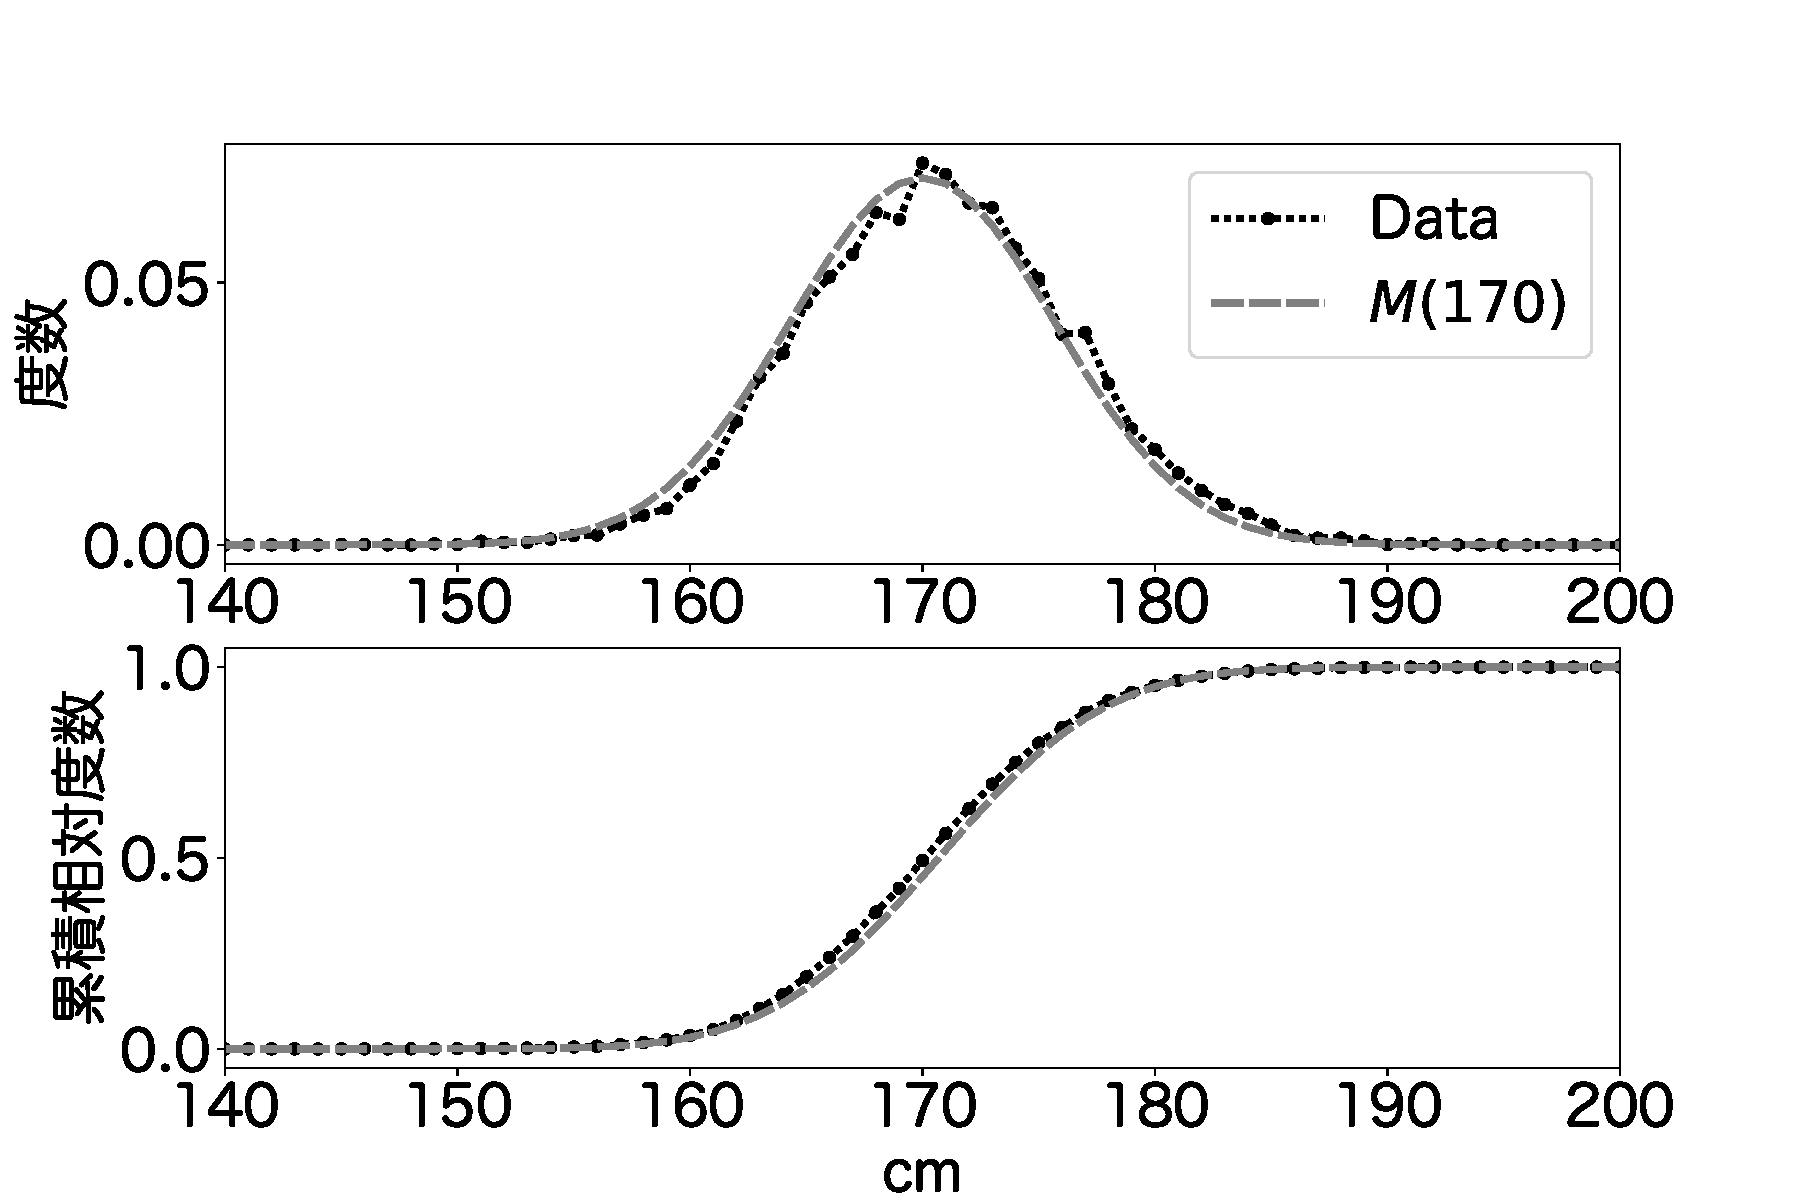
\includegraphics[width=15cm]{./image/03_/cm_data.pdf}
    \caption{17歳の男性から無作為抽出したデータ。上は、データと統計モデル$M(170)$の度数。下は、データと統計モデル$M(170)$の累積相対度数}
    \label{fig:real_height_men}
\end{center}
\end{figure}


\begin{SMbox}{$170cm$を少し超えた人が多いのは、不正(無作為抽出の手順に異常)があったから?}
\begin{quotation}
    「生物学上、グラフは曲線になっていなければならないが、169cmの部分はへこんでいる。これは先生や生徒による四捨五入で生まれるサバ読みの結果。身長が170cmなのか169cmなのかで気持ち的に違ってきますからね」と話すと、食料自給率や犯罪発生件数とは異なる微笑ましいサバ読みのトリックに、出演者一同、笑みを浮かべていた。\footnote{国民を欺く“統計のウソ” 知らないと怖い“統計トリック”を専門家が解説
    \url{https://times.abema.tv/articles/-/5640846} 2022/04/30確認}
\end{quotation}

このように、データが統計モデルに一致しないことから、データに不正な操作が加わっているという推測がされることがある。議論となっている身長のデータを観察してみる。
図\ref{fig:real_height_men}上を見ると、確かに、$170$を超えたあたりの度数は、$169$の度数よりも多い。
また、$170cm$以下のデータは統計モデルの度数よりも低く、$170cm$以上のデータは統計モデルの度数よりも大きい。一方で、図\ref{fig:real_height_men}下の累積相対度数を見ると、度数と同様の変異は少ないように見える。このようなデータと統計モデルの相違の原因は、不正な計測により生じたと断言できるのだろうか。

データとモデルの相違が生じる原因が、不正な計測だけではないことを確認する。
具体的には、データを統計モデルからサンプリングし、そのデータが統計モデルと一致するかを観察してみる(図\ref{fig:simulation_height_men})。図を見るとわかるように、サンプリングを行った場合、$168cm$付近で、度数が曲線よりも上にくる部分がある。また、$170cm$より小さいところでは、統計モデルよりもデータの度数が上にあり、$170cm$より大きなところでは、統計モデルより、データの度数が下にある。このように、統計モデルによりサンプリングし、統計モデルとサンプリングデータを比較した場合でも、ズレが生じる。これは、不正なモデルの予測とデータの間のズレが計測以外から生じることを示唆している。
%単純なズレだけを見たとしても、それが不正なのかは結論をつけることは難しい。


不正を見つけるには、次の経験が必要である。恣意的な操作を一切介入させない、かつ、無作為にデータを取得する条件のもと、得られたデータ、と同じ計測方法・同じ生徒において、教員が計測したデータこの二つのデータが一致しないならば不正な操作が加わったことが疑える。

データ解析をするには、常に、データを収集する手順が守られていないことを疑うことをするべきである。
例えば、髪の毛や靴などを履いる人がそうではない人と同じように計測をされると、平均値が大きくなる。身長の低い生徒に対してその傾向が高ければデータには歪みが生じやすくなる。計測を行なった先生方の疲れなども考慮すれば、データ収集の手順の誤りにより、データが偏ることもある。

データの収集には多大な労力がかかっている。誰かがどこかで腰を痛めながら高校生の身長を測る仕事をしていることは心に留めておくべきで、不正があったと主張するのは、彼らの仕事を低く評価しすぎではないだろうか。おそらく先生たちは、正確に計測できるように正確に手順を満たすように計測しているはずである。
不正を疑うならば、それなりに確証できる証拠を提示すべきである。具体的には、自分が手順を守って計測したデータと、先生が測ったときのデータにおいて、それらの間の差を示すべきである。



もう一つこの論者と私とで異なる点は、生物学データのグラフが曲線になるべきという点である。私は、推論のために統計モデルを利用しているので、統計モデルとデータが一致しない場合でも、推測に利用できると考え、統計モデルを利用する。一方で、この論者は、統計モデルとデータが一致すべきと考えている。言い換えれば、データが統計モデルに従うことを前提にする立場と、データを推論するために統計モデルを仮定すると言う立場がある。

\if 0 
$180cm$以上の割合についてはデータと一致していますが、$160cm$以下は、データと不一致です。この統計モデルで推測できていると考えても良いのでしょうか。
無作為抽出したときに得られるデータをできます。
ここで、$\mu=169.1$の統計モデル$M(\mu=169.1)$と、$\mu=180$の統計モデル$M(180)$を
標本から無作為抽出を行い、集計すると平均$169.1cm$程度であることがわかったとします。このとき統計モデル$M(169.1)$の推測は母集団の特徴をよく捉えているだろうか?
\fi 
\end{SMbox}

\begin{figure}
    \begin{center}
        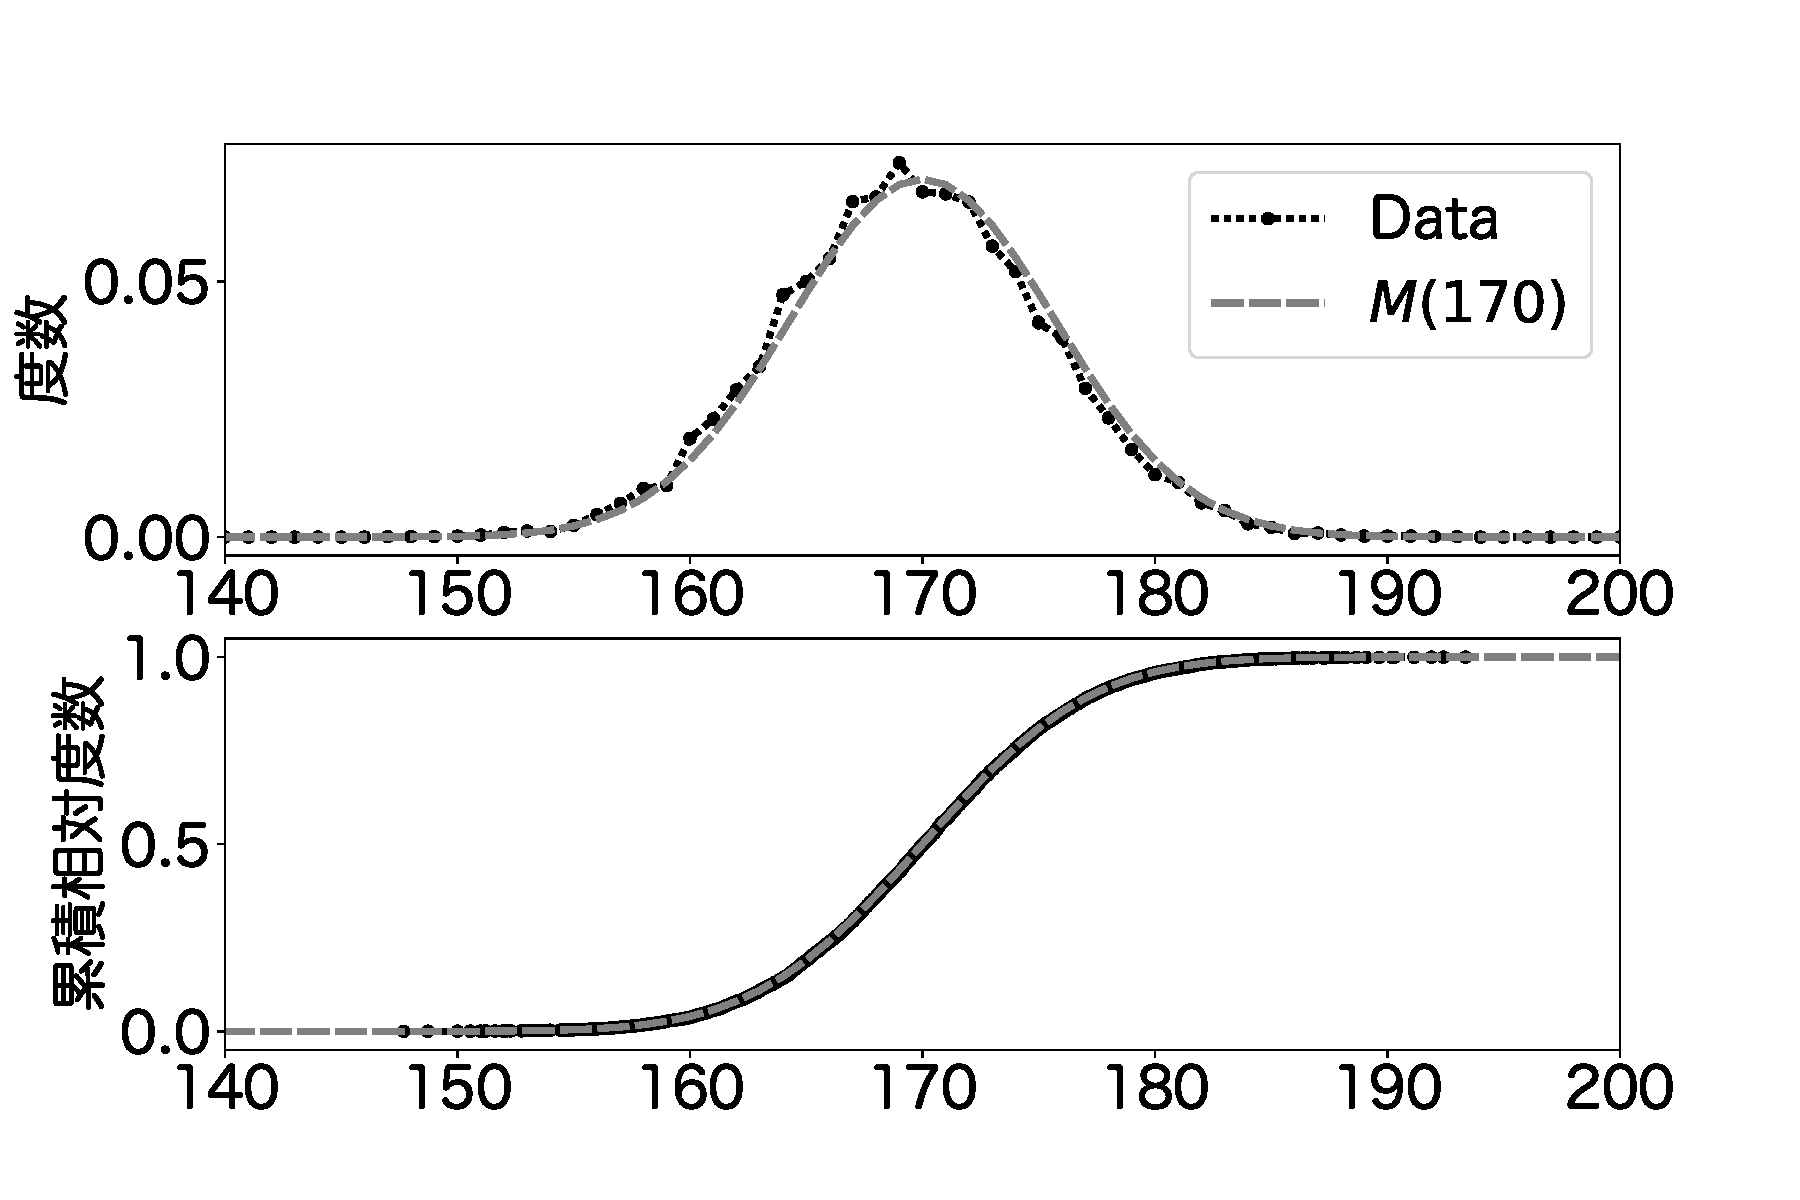
\includegraphics[width=15cm]{./image/03_/cm_data_simulation.pdf}
        \caption{上:正規分布を含む統計モデル$M(170)$によりサンプリングされたDataの頻度と、統計モデルの頻度。下:上と同じデータ・統計モデルの累積相対頻度}
        \label{fig:simulation_height_men}
    \end{center}
\end{figure}

\begin{SMbox}{軽いパンばかり買わされる}
ある国では、ある時期、パンを作るための道具、手順、材料が政府からパン屋に配布され、パン屋がパンを作ることになっていた。パンを焼くための型は、完成時に$1000g$になるように設計されており、手順を厳密に守り作ったパンは確かにおよそ$1000g$になっていた。どの季節に作っても手順を守りさえすれば、$1000g$になったのだ。
この材料、道具をパン屋が利用し、手順にそってパンを作れば、やはりパンはおよそ$1000g$になるはずである。

その国では、小麦の値段が高騰しており、支給された小麦をそのまま売った方が儲かるという状況になっていた。そんなとき、パンが$1000g$よりも軽いと感じた数学者が、数ヶ月にわたりパンの重量を計測していった。その結果、パンの重量は平均で$950g$となっており、本来の$1000g$よりも、軽いことがわかった。

このとき、パン屋が不正をしていると主張できる。
手順を踏めば平均で$1000g$になるパンが平均およそ$950$になったのは、パン屋が手順通りにパンを作っていないことを疑える。手順を守って作れば$1000g$になるという経験(データ)があるから疑うことができる。
%もしも、季節によってパンの重さが変化するものだったとするなら、$4$月には$1000g$だったものが$6$月には、$900g$になる可能性を排除できない。
\end{SMbox}


\subsection{サンプルサイズが大きい場合}

データと統計モデルを比較する。$180cm$以上の割合は、0.0642であり、モデル$M(171.1)$の推測値$P(x>180)=0.059$と数値が近い。
また$160cm$以下の割合は、$0.023$程度であり、統計モデルの推測値$P(x<160)=0.025$であり、やはり数値が近い。
%このように数学的フィクションである統計モデルを使うことで、現実に関する推測が可能になった。

ここまでは、$M(171.1)$を用いて、母集団を推測した。統計モデル$M(170)$の代わりに$M(168)$により推測を行うとデータとの一致具合を確かめる。$180cm$以上の人を推測すると$M(168)$では$P(x>180)=0.03$であり、統計モデル$M(171.1)$の推測$P(x>180)=0.059$よりもさらに実際の計測値$0.0642$と乖離している。
これは、$M(168)$では、ピークが平均値の$168$に移動するので、$180cm$を超える割合がさらに低くなるので、実際の数値から離れる。

一方で、$160$以下の人では、$M(168)$では、$P(x<160)=0.08$程であり、$M(171.1)$の推測値$P(x<160)=0.025$よりも、実際の数値$0.023$から離れている.
これも、$M(168)$では、ピークが$170$よりも小さな値になるので、$160cm$より小さい人の割合が大きくなるので、予測と実際のデータの不一致度が大きくなる(表\ref{table:data_type}にまとめておいた)。
このように、統計モデルの母数に応じて、現実の予測精度が変化する。

\begin{table}[hbtp]
    \caption{統計モデルとデータの比較}
    \label{table:data_type}
    \centering
    \begin{tabular}{lcc}
    %\hline
    統計モデル  & $P(x<160)$  & $P(x>180)$   \\
    \hline \hline
    データ &  0.023 &  0.0642\\
      %\hline \hline
    M(171.1) & 0.025 & 0.059  \\
    M(168) &  0.08 & 0.03 \\
      \hline
    \end{tabular}
  \end{table}


この統計モデルの予測の良さが分かったのは、無作為抽出を繰り返して、サンプルサイズを大きくしたときのデータの分布を得ていることによって、
そのデータとモデルとを比較をすることで、$M(171.1)$が$M(168)$より良い統計モデルであることを判別できた。

では、データが十分でない場合においても、推測とデータの一致を基準にして、より良い統計モデルを選ぶことはできるのでしょうか?

\subsection{サンプルサイズが小さい場合}
%\subsection{推測値とデータの比較}
母集団のことをほとんど知らない場合において、統計モデルとデータの比較はできるが、これを元に統計モデルが良いことを検討できない。
\if 0
母集団に関して次のことを知っていることにします。
\begin{itemize}
    \item 平均がおよそ$170cm$
    \item $160cm$の人や$180cm$の人と出会う確率は同じくらい($170cm$を中心に対象に分布している)
    \item 分散は5.7
\end{itemize}
\fi
サンプルサイズ10の標本が二つ得られたとします(実際には、コンピュータを使って正規分布からサンプリングした。このデータは母集団から無作為抽出したと考える)。標本は、次の通り。

\begin{lstlisting}
sample1 = [162.56944902, 178.42128764, 171.15286336, 172.2581195 , 160.21499345, 175.35072013, 173.17952774, 173.73301156, 179.52758126, 178.35924221]
\end{lstlisting}

\begin{table}[hbtp]
  \caption{統計モデルと小さいサンプルサイズの標本}
  \label{table:smalle_sample_size}
  \centering
  \begin{tabular}{lccc}
  %\hline
  統計モデル  & $P(x<160)$  & $P(x>180)$  & $\bar{X}$ \\
  \hline \hline
  標本1 &  0 &  0 & 172.8 \\
    %\hline \hline
  M(171.1) & 0.025 & 0.059  & 171.1 \\
  M(168) &  0.08 & 0.03 & 168\\
    \hline
  \end{tabular}
\end{table}
$180cm$以上の人は、$0$人、$160cm$以下の人も$0$人、どちらの統計モデルでも推測と一致しているかを推測できない[表\ref{table:smalle_sample_size}]。
標本平均$\bar{X}=172.8$であり、$M(170)$の母数$170$が$M(168)$の母数平均$168cm$でどちらも同じ程度の差である。
サンプルサイズが小さいときには、統計モデルの予測とデータを比較できないことがあるので、予測精度の良いモデルがどれかを決定できないことがある。


\if 0
sample2 = [164.04222157, 162.19052559, 172.03420244, 168.03580415, 176.73750537, 166.41177205, 165.27050656, 168.02537023, 176.18720054, 171.78005419]
\end{lstlisting}


\begin{table}[hbtp]
    \caption{統計モデルと小さいサンプルサイズの標本}
    \label{table:smalle_sample_size}
    \centering
    \begin{tabular}{lccc}
    %\hline
    統計モデル  & $P(x<160)$  & $P(x>180)$  & $\bar{X}$ \\
    \hline \hline
    標本1 &  0 &  0 & 172.8 \\
    標本2 &  0 &  0 & 169 \\
      %\hline \hline
    M(171.1) & 0.025 & 0.059  & 171.1 \\
    M(168) &  0.08 & 0.03 & 168\\
      \hline
    \end{tabular}
  \end{table}
どちらの標本でも

\fi
% また、標本の平均値と統計モデルの平均値でも標本が
% 仮説検定の枠組みでは、絶対にだめな統計モデルを明らかにします。

%\subsubsection{標本内の偏った値に注目}

%\section{統計モデルの比較 尤度・対数尤度}

\section{統計モデルとデータの比較 2}


\subsection{モデルの平均を含む信頼区間の個数}
実際に、$M(\mu=170)$を使って、$サンプルサイズを10$とし、標本を$100$個作ってみると、
その標本平均の分布は、図\ref{fig:confidence_interval_sample}Bである。
それぞれの標本に対して、最尤モデル$M(\bar{x}_i)$を作り、信頼区間を描いたものが図\ref{fig:confidence_interval_sample}Aである。
図\ref{fig:confidence_interval_sample}Aの170cmのところにある縦の線は、元の統計モデル$M(\mu=170)$の母数平均である。
元の統計モデルの母数170cmを跨いでいる信頼区間の個数はこの図では$96$個ある。コンピュータシミュレーションをすると、$\mu$を跨いでいる信頼区間の個数はおよそ95個である。
このことは、信頼区間の定義から明らかである。

\begin{figure}
\begin{center}
    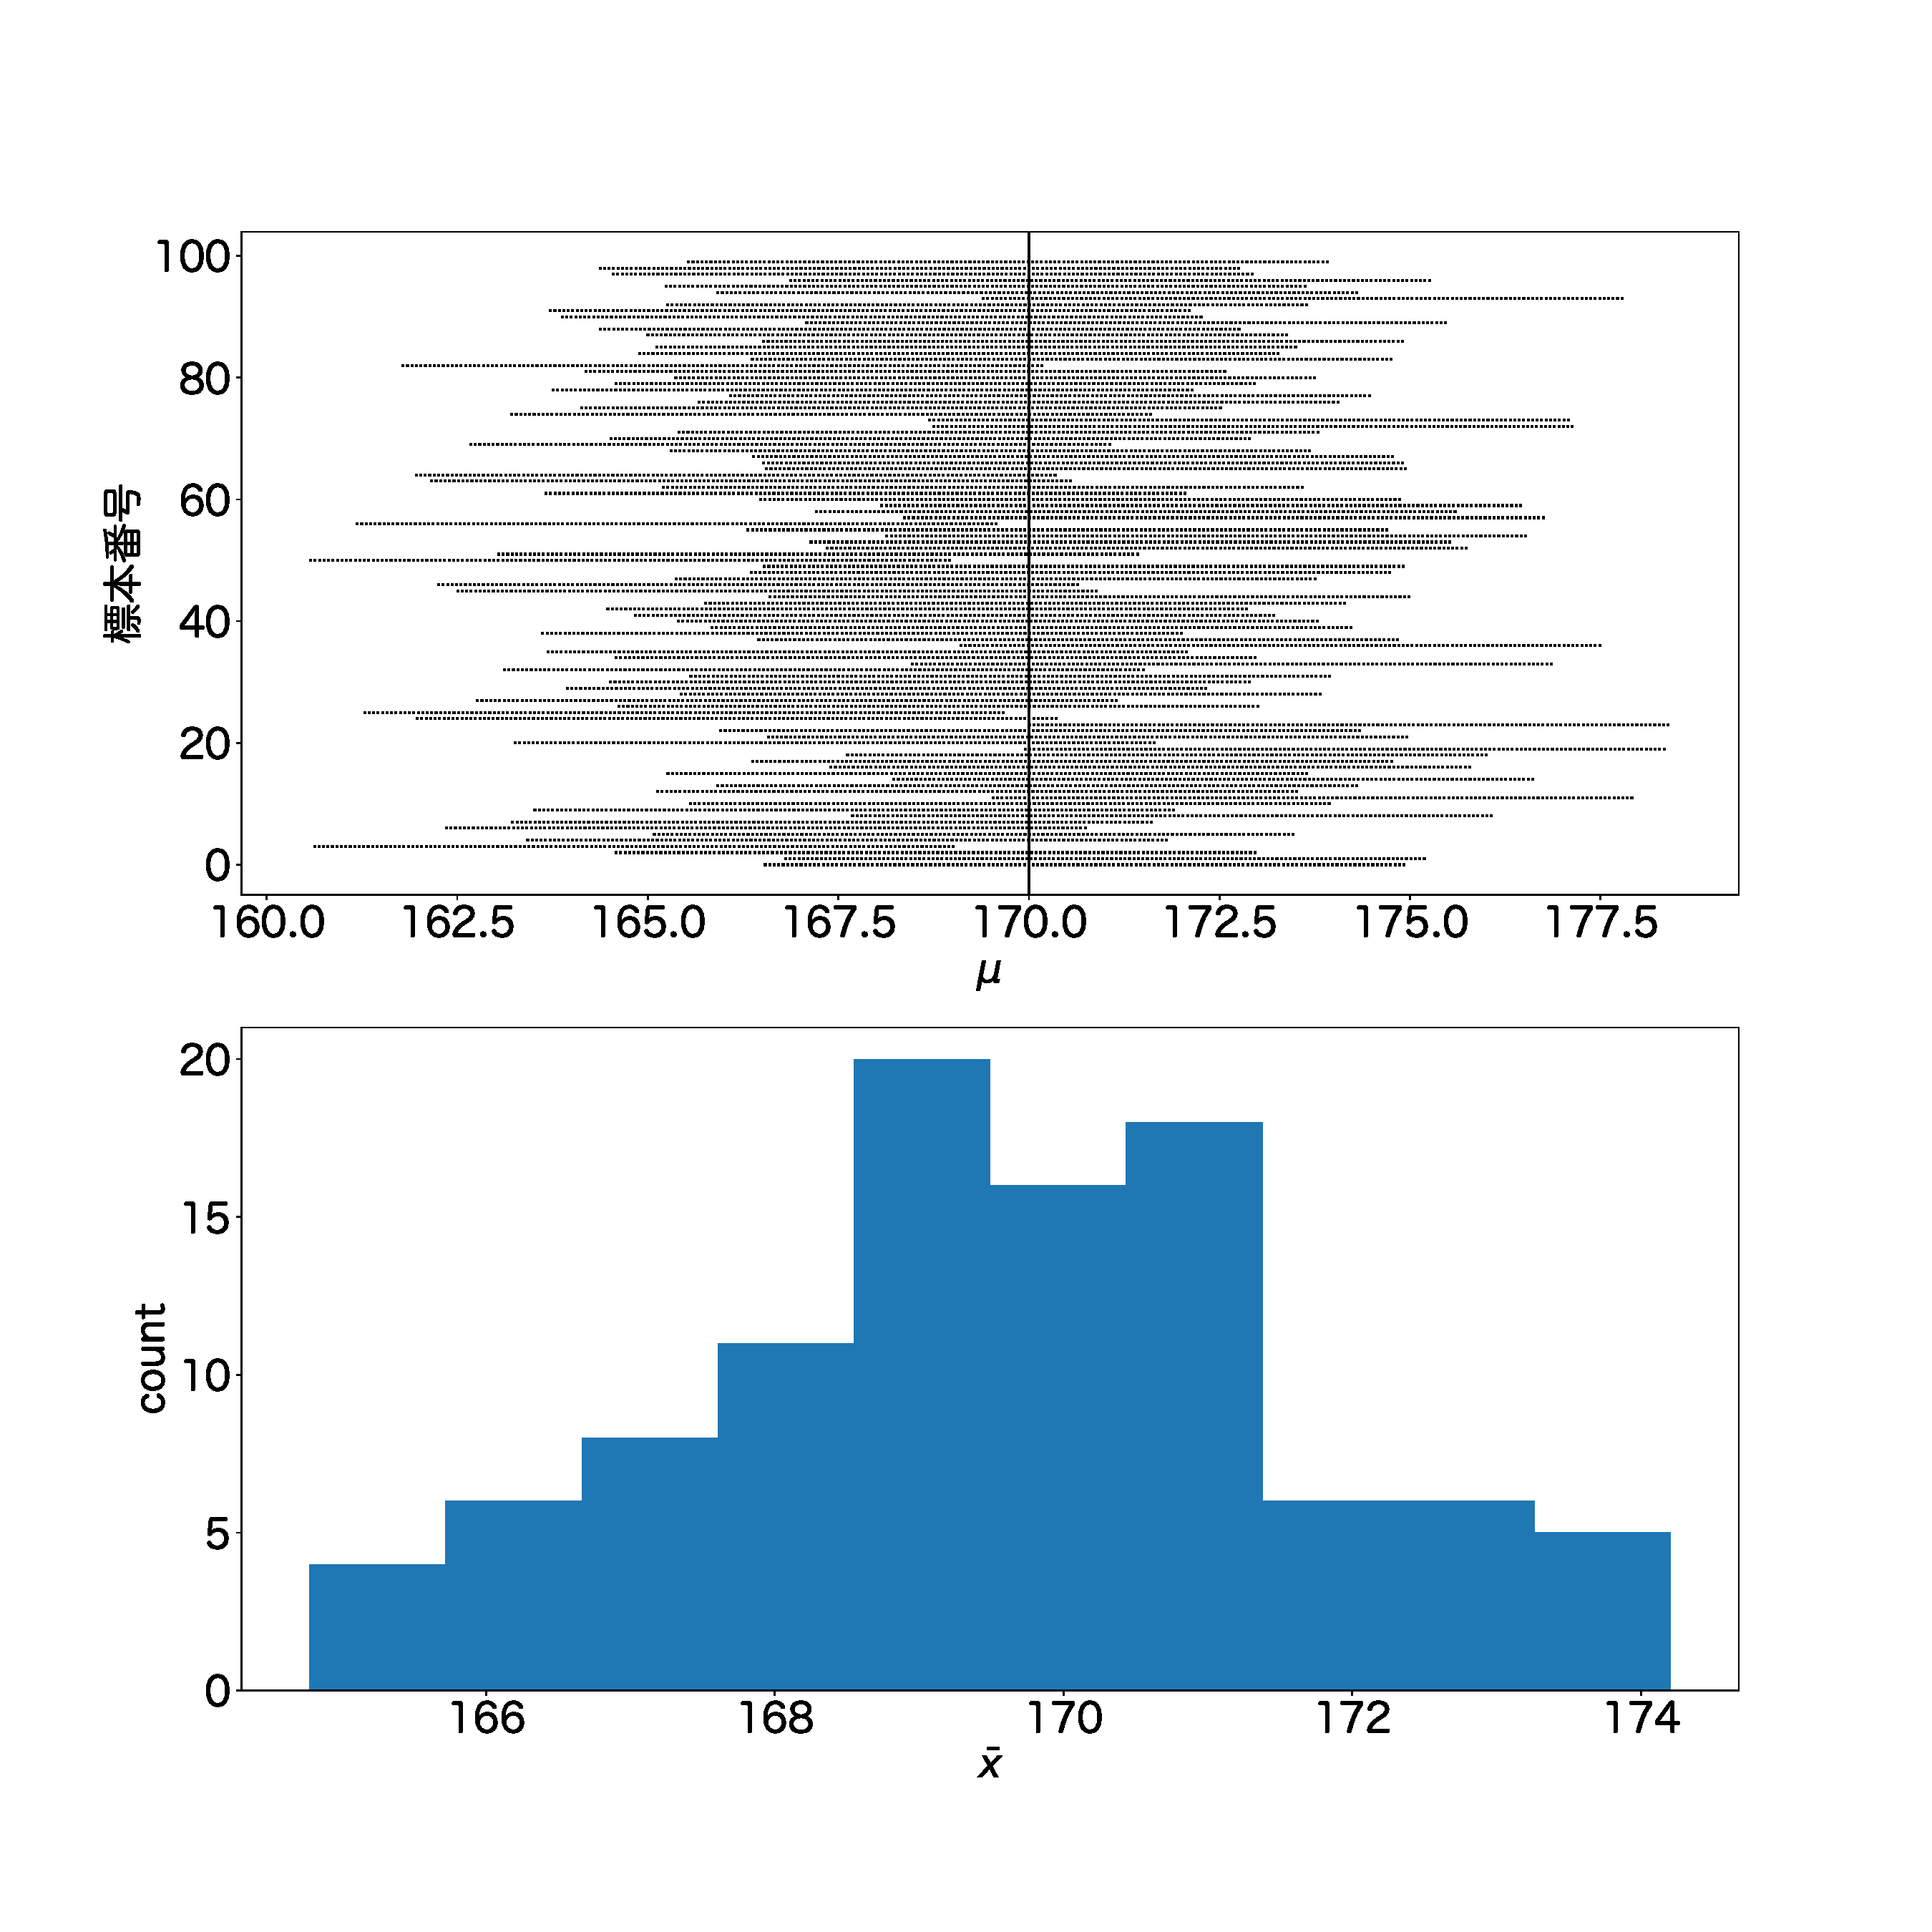
\includegraphics[width=15cm]{./image/03_/confidence_interval_model_count.pdf}
    \caption{(A)モデルから標本を得て、その標本から信頼区間を計算し、表示したもの。(B)標本平均の分布}
    \label{fig:confidence_interval_sample}
  \end{center}
\end{figure}


\begin{SMbox}{信頼区間は、データをたくさん取ったときに(サンプルサイズが同じ標本をたくさん集めたときに)、その範囲に真値が$95\%$の確率で含まれるの区間のこと}
信頼区間は、データをたくさん取ったときに、その範囲に真値が入る$95\%$の確率で含まれるの区間のこと\footnote{\url{https://www.slideshare.net/simizu706/ss-123679555}}。このように解説されることがある。
データを元に、統計モデルの母数を決定したときに、信頼区間が得られる。さらに計測を行い標本を作ると、標本の標本平均がこの信頼区間の間に含まれる確率が$95\%$であることを主張していると考えられる。

一般に、母集団が統計モデルにより、よく推測できるならば、無作為抽出の標本平均が$95\%$くらいの確率で信頼区間に含まれる。そうではないならば、$95\%$信頼区間にモデルの母数が含まれる確率は$95\%$とは異なる値をとることがある。
モデルが推測に適さないことは科学においてはよくあり、この解釈は科学においてはやめておいた方が良いと考えられる。 

統計科学の一部では、データをたくさんとったときに\footnote{モデルからサンプリングしていない}、信頼区間内に真値が$95\%$の確率で含まれる区間と解釈されることがあるということは心に留めておくと、統計学者との会話が可能になる。
\end{SMbox}



%\subsection{推測に利用できないと判定する}

\if 0
$N=1$では、$\bar{x}$が$154\sim185$あたりであれば、$M(170)$は棄却できない。$N=4$であれば、$\bar{x}$が$162\sim177$であれば、$M(170)$は棄却できない。$N=10$であれば、$\bar{x}$が$165\sim174$であれば、$M(170)$は棄却できない。
このようにサンプルサイズが増加することで、信頼区間が狭まり、棄却できるモデルの母数の範囲が狭まることがわかる。
\fi

\section{統計検定量によるモデルの評価}

これまでは、統計モデル$M(\mu)$における信頼区間・棄却域の計算を行った。今回は、$p$値を計算する。
無作為抽出により得られたデータ$\bar{x}$がこれ以上偏る確率は、
$\phi(z>\frac{\sqrt{n}(\bar{x}-\mu)}{\sigma})$
である。



棄却されるモデルが観測されたデータの平均値$\bar{x}$に応じて変化することを視覚的に確認しておく。図はさまざまな$\bar{x}$を得たときにその信頼区間を描いたものである。この信頼区間の範囲内にある$\mu$であれば、統計モデル$M(\mu)$は棄却されない。例えば、$\bar{x}=170$であれば、$M(170)$は棄却されない。一方で、$\bar{x}=165$あたりであれば、その棄却域は$\mu=170$を含まないので、$M(170)$は棄却される。


\subsection{データの統計検定量と統計モデルの評価}
%母集団から無作為抽出したデータについて考えます。
実際の標本のサンプル$X_1,X_2,\cdots,X_{10}$について、その標本平均を$\bar{X}$とする。$M(\mu=171)$において、$\bar{X}$以上の値が得られる確率を計算する。
$\phi(z)$を標準正規分布とすると、$\phi(z>\frac{\sqrt{n}(\bar{x}-\mu)}{\sigma})$を計算する。
具体的な数値として、
$\bar{X}=172$モデルの母数を$\mu=171$なら、$p=\phi(z>\frac{\sqrt{n}(\bar{x}-\mu)}{\sigma}) = 0.289$であり、$\bar{X}=169$、モデルの母数を$\mu=171$の場合、$p=\phi(z>\frac{\sqrt{n}(\bar{x}-\mu)}{\sigma}) = 0.866$である。統計モデル$M(\mu=171)$において、これらの標本平均は、そこまで珍しいものではない。
\if 0
実際に、検定を行なっておく。$N=1,\bar{x}=181$とする。このとき、$\bar{x}\sim N(\mu,\sigma^2)$より、$\frac{\sqrt{n}(170-\bar{x})}{\sigma}=-1.61$より、$z_{0.975}=-2.241$なので、棄却域に含まれない。統計モデル$M(170)$は棄却されない。
$N=4,\bar{x}=181$とする。このとき、$\frac{\sqrt{n}(170-\bar{x})}{\sigma}=-3.23$より、棄却されることがわかる。
\fi
言い換えれば、このモデルにより、母集団について予測ができるかもしれないことを示唆している。
%$M(168)$でも同様に計算できる。

\begin{lstlisting}
    xbar = 172
    mu=171
    sigma = 5.7
    N=10
    c = np.sqrt(N)*(xbar-mu)/sigma
    1-norm.cdf(c,0,1)
\end{lstlisting}

\subsection{標本平均と$p$値}
$M(171)$の上で、各$\bar{X}$に対して$p=\phi(z>Z(\mu))$を計算する。
これを図示したのが図\ref{fig:p_cm}である。
標本平均$171cm$をピークに左右対象に$p$値が減少している。
モデルの母数$\mu$と$\bar{X}$が近ければ、$p$値が大きく、離れるほど$p$値が小さい。
言い換えると、得られたデータが統計モデルによって推測できそうであれば、$p$値が小さく、離れるほど$p$値が小さくなる。
このことから、$p$値が一つの目安になることが示唆される。

\begin{figure}
\begin{center}
   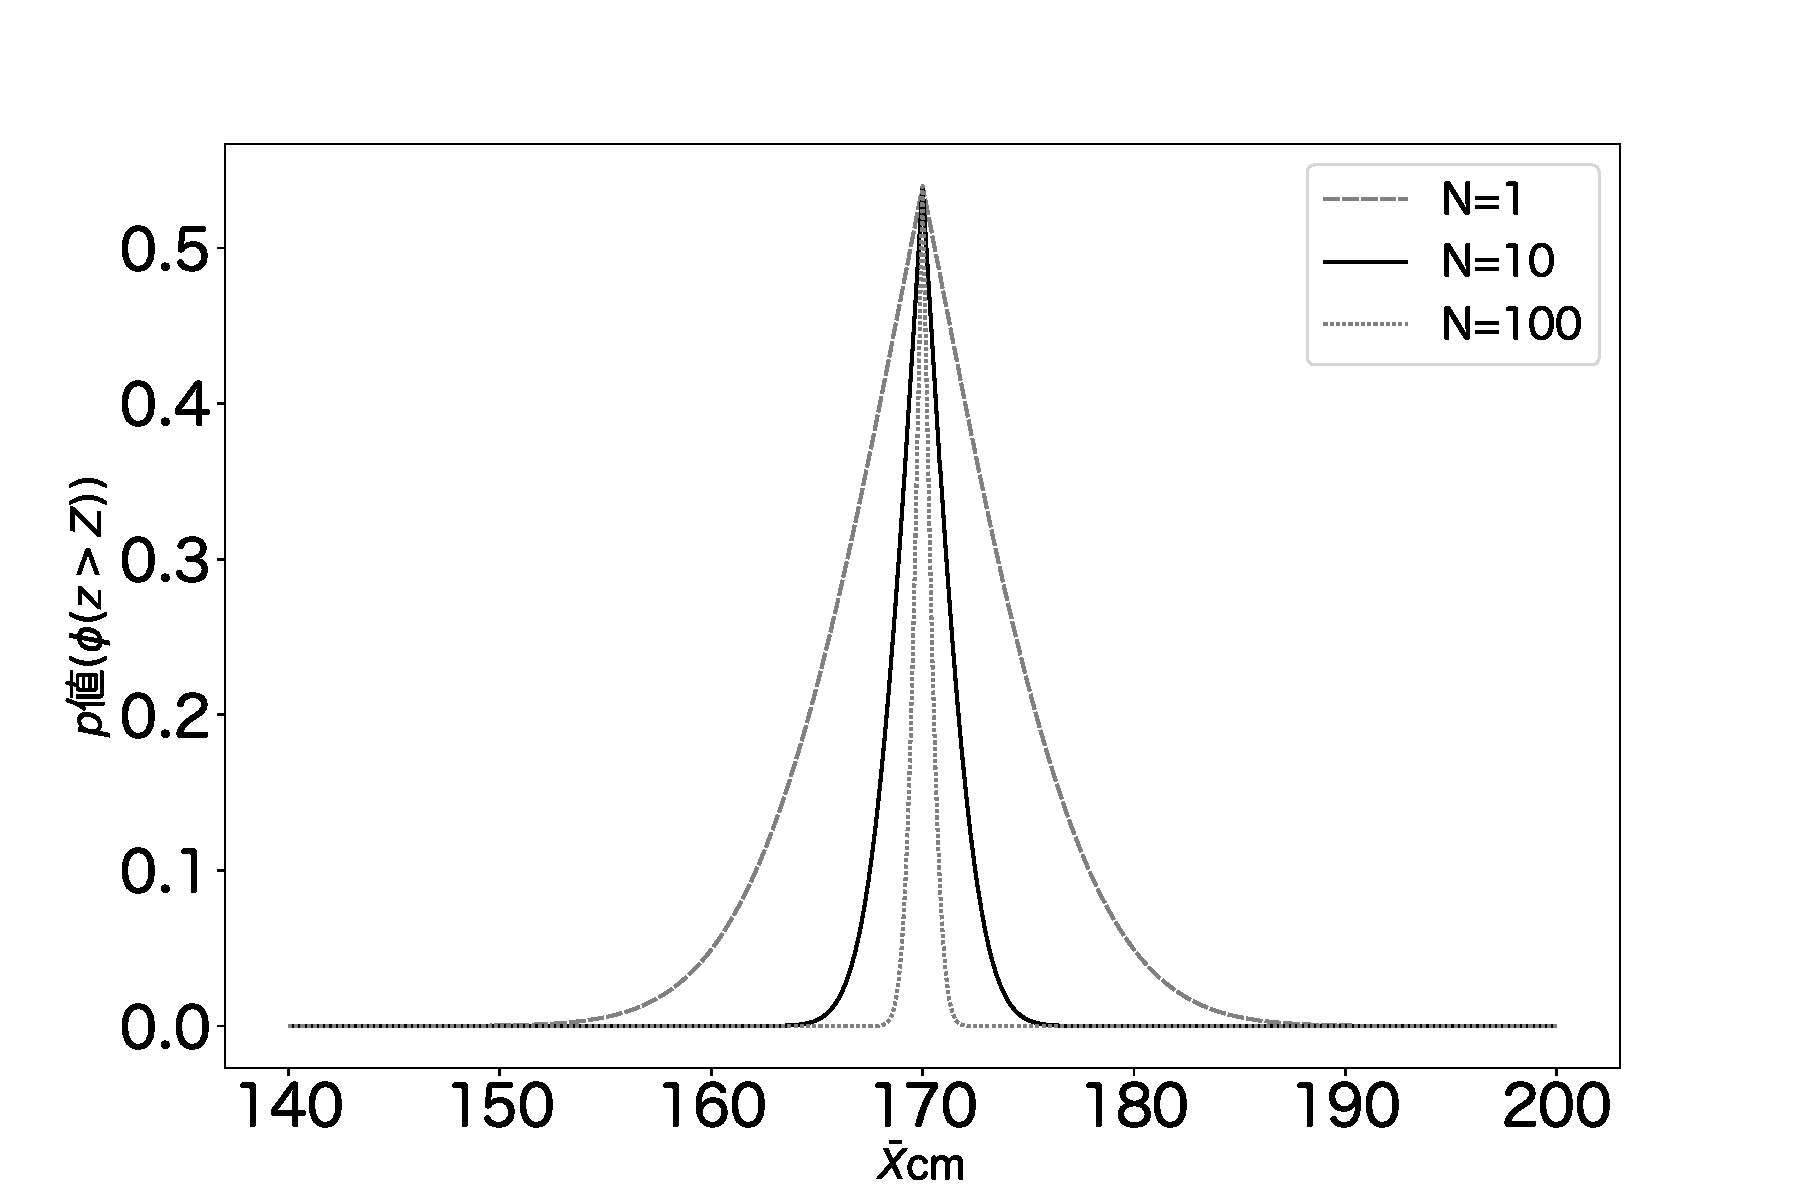
\includegraphics[width=15cm]{./image/04_/p_cm.pdf}
   \caption{各標本平均$\bar{X}$が$M(\mu=171)$において得られる確率。$N=1,10,100$の場合。}
   \label{fig:p_cm}
 \end{center}
\end{figure}





%\section{データを元にした統計モデル}
%\subsection{最尤推定}

%\subsection{aaa}

%\subsection{推定した母数を持つモデルとそのほかのモデル}


%
\chapter{指数分布を使った統計モデル}
あるシステムの故障発生間隔日数を調べてみると、次のようなデータを得たとする(実際には、平均10の指数分布関数を使いサンプリングを行った。もちろんそんなことは忘れて、現象は数学関数により生成されていないと考える)
\begin{lstlisting}
19.9290003   0.60892905  0.55864947 29.77846887  0.28955969  1.58223429 21.10080586 10.78952122  0.59624638 15.74379646
\end{lstlisting}


平均値は10.09,分散は107.7であった。以下の仮定からなる統計モデルを構築した。
\begin{quote}
    \begin{enumerate}[(1)]
\item i.i.d
\item 正規分布
\item 平均10.09、分散107.7
\end{enumerate}
\end{quote}
では統計量を元に、$p$値を求めてみる。具体的には、

\begin{lstlisting}
Y =[19.9290003 ,  0.60892905,  0.55864947, 29.77846887,  0.28955969,  1.58223429, 21.10080586, 10.78952122,  0.59624638, 15.74379646]
stats.ttest_1samp(Y, 10.09)
\end{lstlisting}

結果、$p=0.978$である。$p=0.05$を基準にすれば、この統計モデルは棄却できない。統計モデルの仮定が妥当かを一つずつ調べる。統計モデルの仮定(2)は、分布が正規分布であることを仮定している。実際の標本をQ-Qプロットしてみよう。正規分布だと考えても問題がなさそうである。統計モデルの仮定(3)について検討する。このサンプルの平均値は$10.09$なので、これについても仮定は妥当だと考えられる。
では、帰無仮説を採択し、この統計モデルを元に推測をするべきだろうか。このモデルで推測を行なってみる。$15$日後の故障発生率は$P(X>20)=0.0036$程度である。同様に、$5$日後の故障発生率は、$P(X>5)=0.0036$である。正規分布は左右対称な関数なので、平均故障発生日から5日でも15日でも、同じ割合で故障する。 
機械などの故障は日数がたてば故障しやすくなるので、肌感覚としてあり得ないと思われる。
実際に、この統計モデルによる故障発生間隔の推測は現実と乖離していくことがわかっている。
このように、恣意的に決めた$p$より大きな統計モデルを使ったとしても、推測がうまくいくわけではないことから、棄却されなかった統計モデルを採用することには慎重になるべきである。

二つ目は、データの偏りによって、統計モデルを棄却できないことあるということである。
$10000$回実験を繰り返したとして(もちろん、指数分ぷからサンプリングを行った。もちろんそんなことは忘れて、現象は数学関数により生成されていないと考えてください)、サンプルサイズは毎回10だとすると、棄却できる割合は0程度であった。一方で、サンプルサイズを$100$程度にすると、棄却できる割合は、$0.956$程度であった。これは、平均値のあたりにデータが集まりやすく、データの端は無視できる程度の数量しか発生しないことで、正規分布を使った統計モデルを棄却しにくくなる。TODO
このように、データが十分ない場合は$p$の棄却に正規分布を仮定した統計モデルでは統計モデルを棄却する頻度は高くなることが予想される。

$p$値による判断がうまくいかないことがわかった。また、信頼区間の中にある母数でも推論ができないこともわかった。
\if 0
このような偏ったデータを手に入れた場合はどのように統計モデルを作ればいいのだろうか。
\fi

https://biolab.sakura.ne.jp/small-sample-t-test-glm.html



\subsubsection{モデルの更新}
\if 0
データ数の問題と、推測の精度の問題を解決することはできるだろうか?
尤度ひ検定
\fi
月日は流れ、データが蓄積された。その結果、次のような分布が得られた。ここまでの議論で、正規分布を仮定したモデルを棄却できないことはわかった。では、そのモデルを使って現在のデータを予測できるだろうか?パラメータを推定した正規分布とデータの分布を見てみよう。
データの最頻値が0の近くなので、平均10の正規分布では、ズレが生じることがわかる。
これではデータを捉えることはできない。
また、$30$日後までに故障が発生する確率を計算してみると、$0.971$程度であり、30よりも大きなデータの数は$0.05(1-0.05=0.95)$それなりに良く一致している。
一方で,5日までの故障発生率は、$0.30$をと予測するが、実際のデータは、0.18程度であり、こちらは乖離していると感じるだろう。
\begin{figure}
\begin{center}
    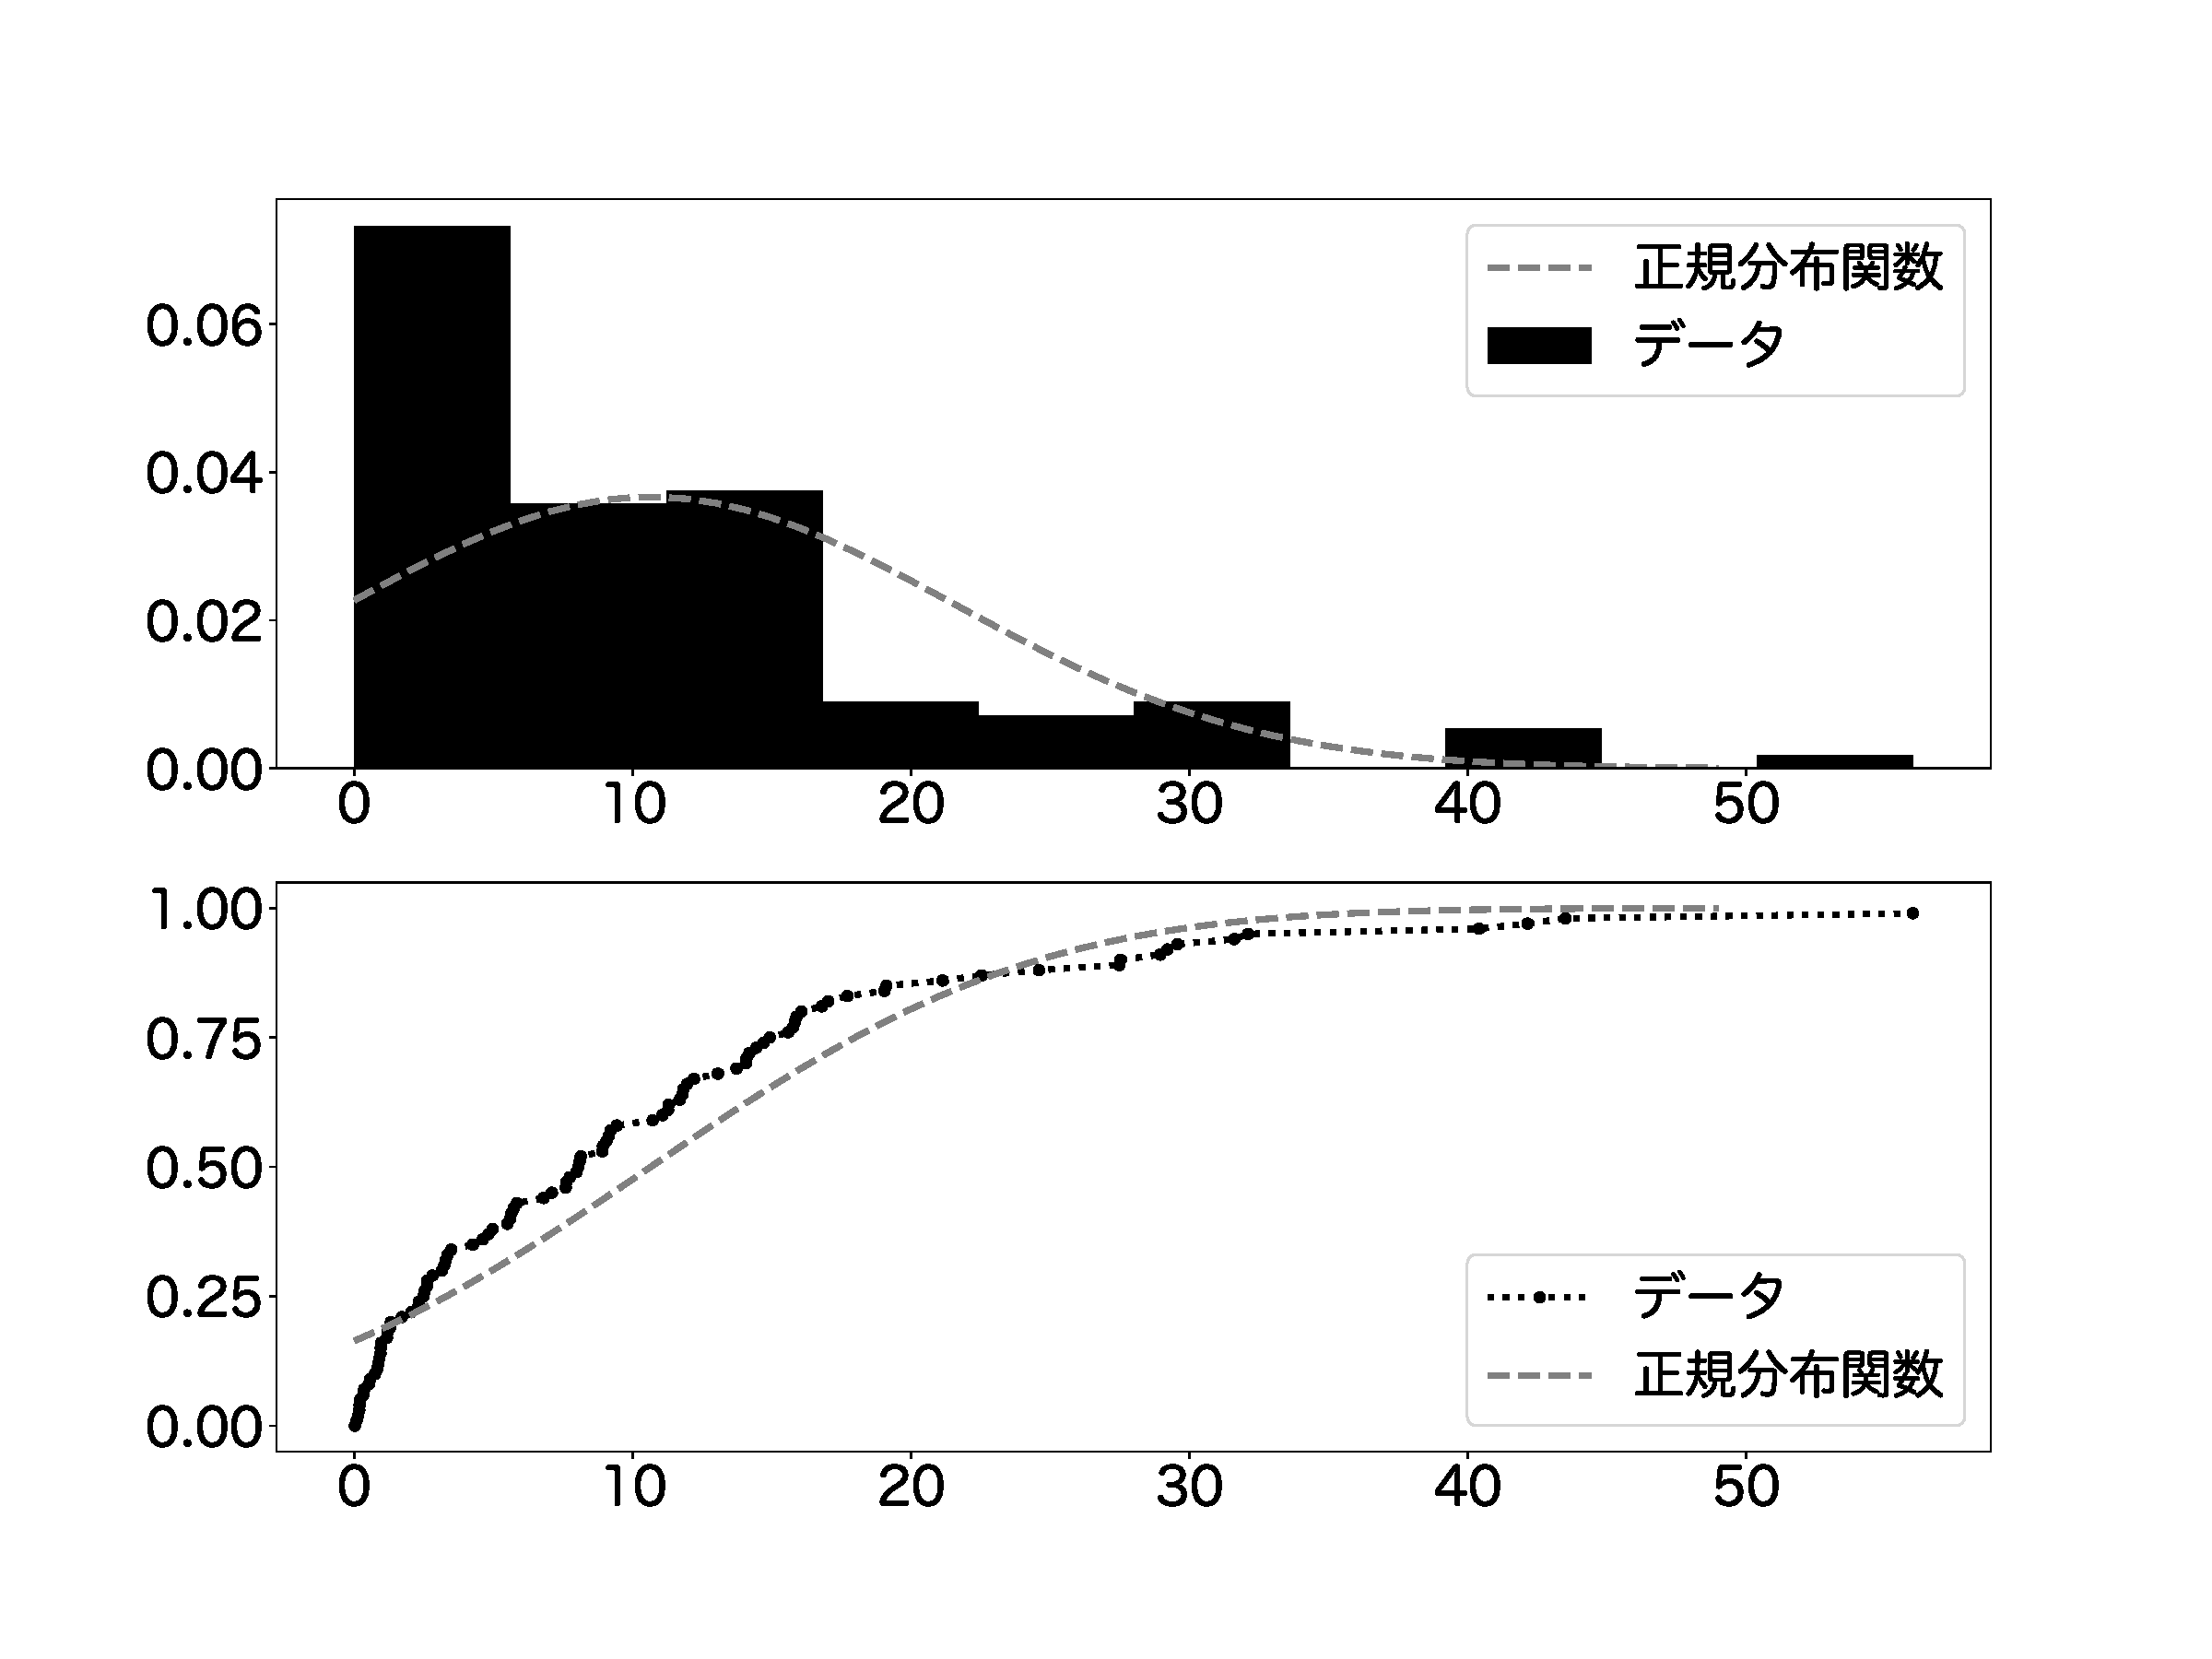
\includegraphics[width=15cm]{./image/06_/normal_exponential.pdf}
    %\caption{データの分布を正規分布で捉えれない}
\end{center}
\end{figure}


では、どのようなモデルを構築すればいいのだろうか。指数分布関数を使ってみよう
\begin{quote}
    \begin{enumerate}[(1)]
\item i.i.d
\item 指数分布
\item 母数$\lambda$
\end{enumerate}
\end{quote}
このモデルを$M(\lambda)$とかく。指数分布では、確率変数の平均は、母数$\lambda$の逆数であることがわかっている($E[x]=\frac{1}{\lambda}$)。$\lambda$として、現在手に入れたデータの平均値の逆数を代入し、データの分布と指数関数の曲線を書いてみると、よく一致しているように見える。

30日後に故障が起こる可能性は、$0.94$程度であると予想が出る。現状のデータと確認をしてみると、30よりも大きなデータの数は$0.05(1-0.05=0.95)$より、良く一致していることもわかる。
\begin{figure}
\begin{center}
    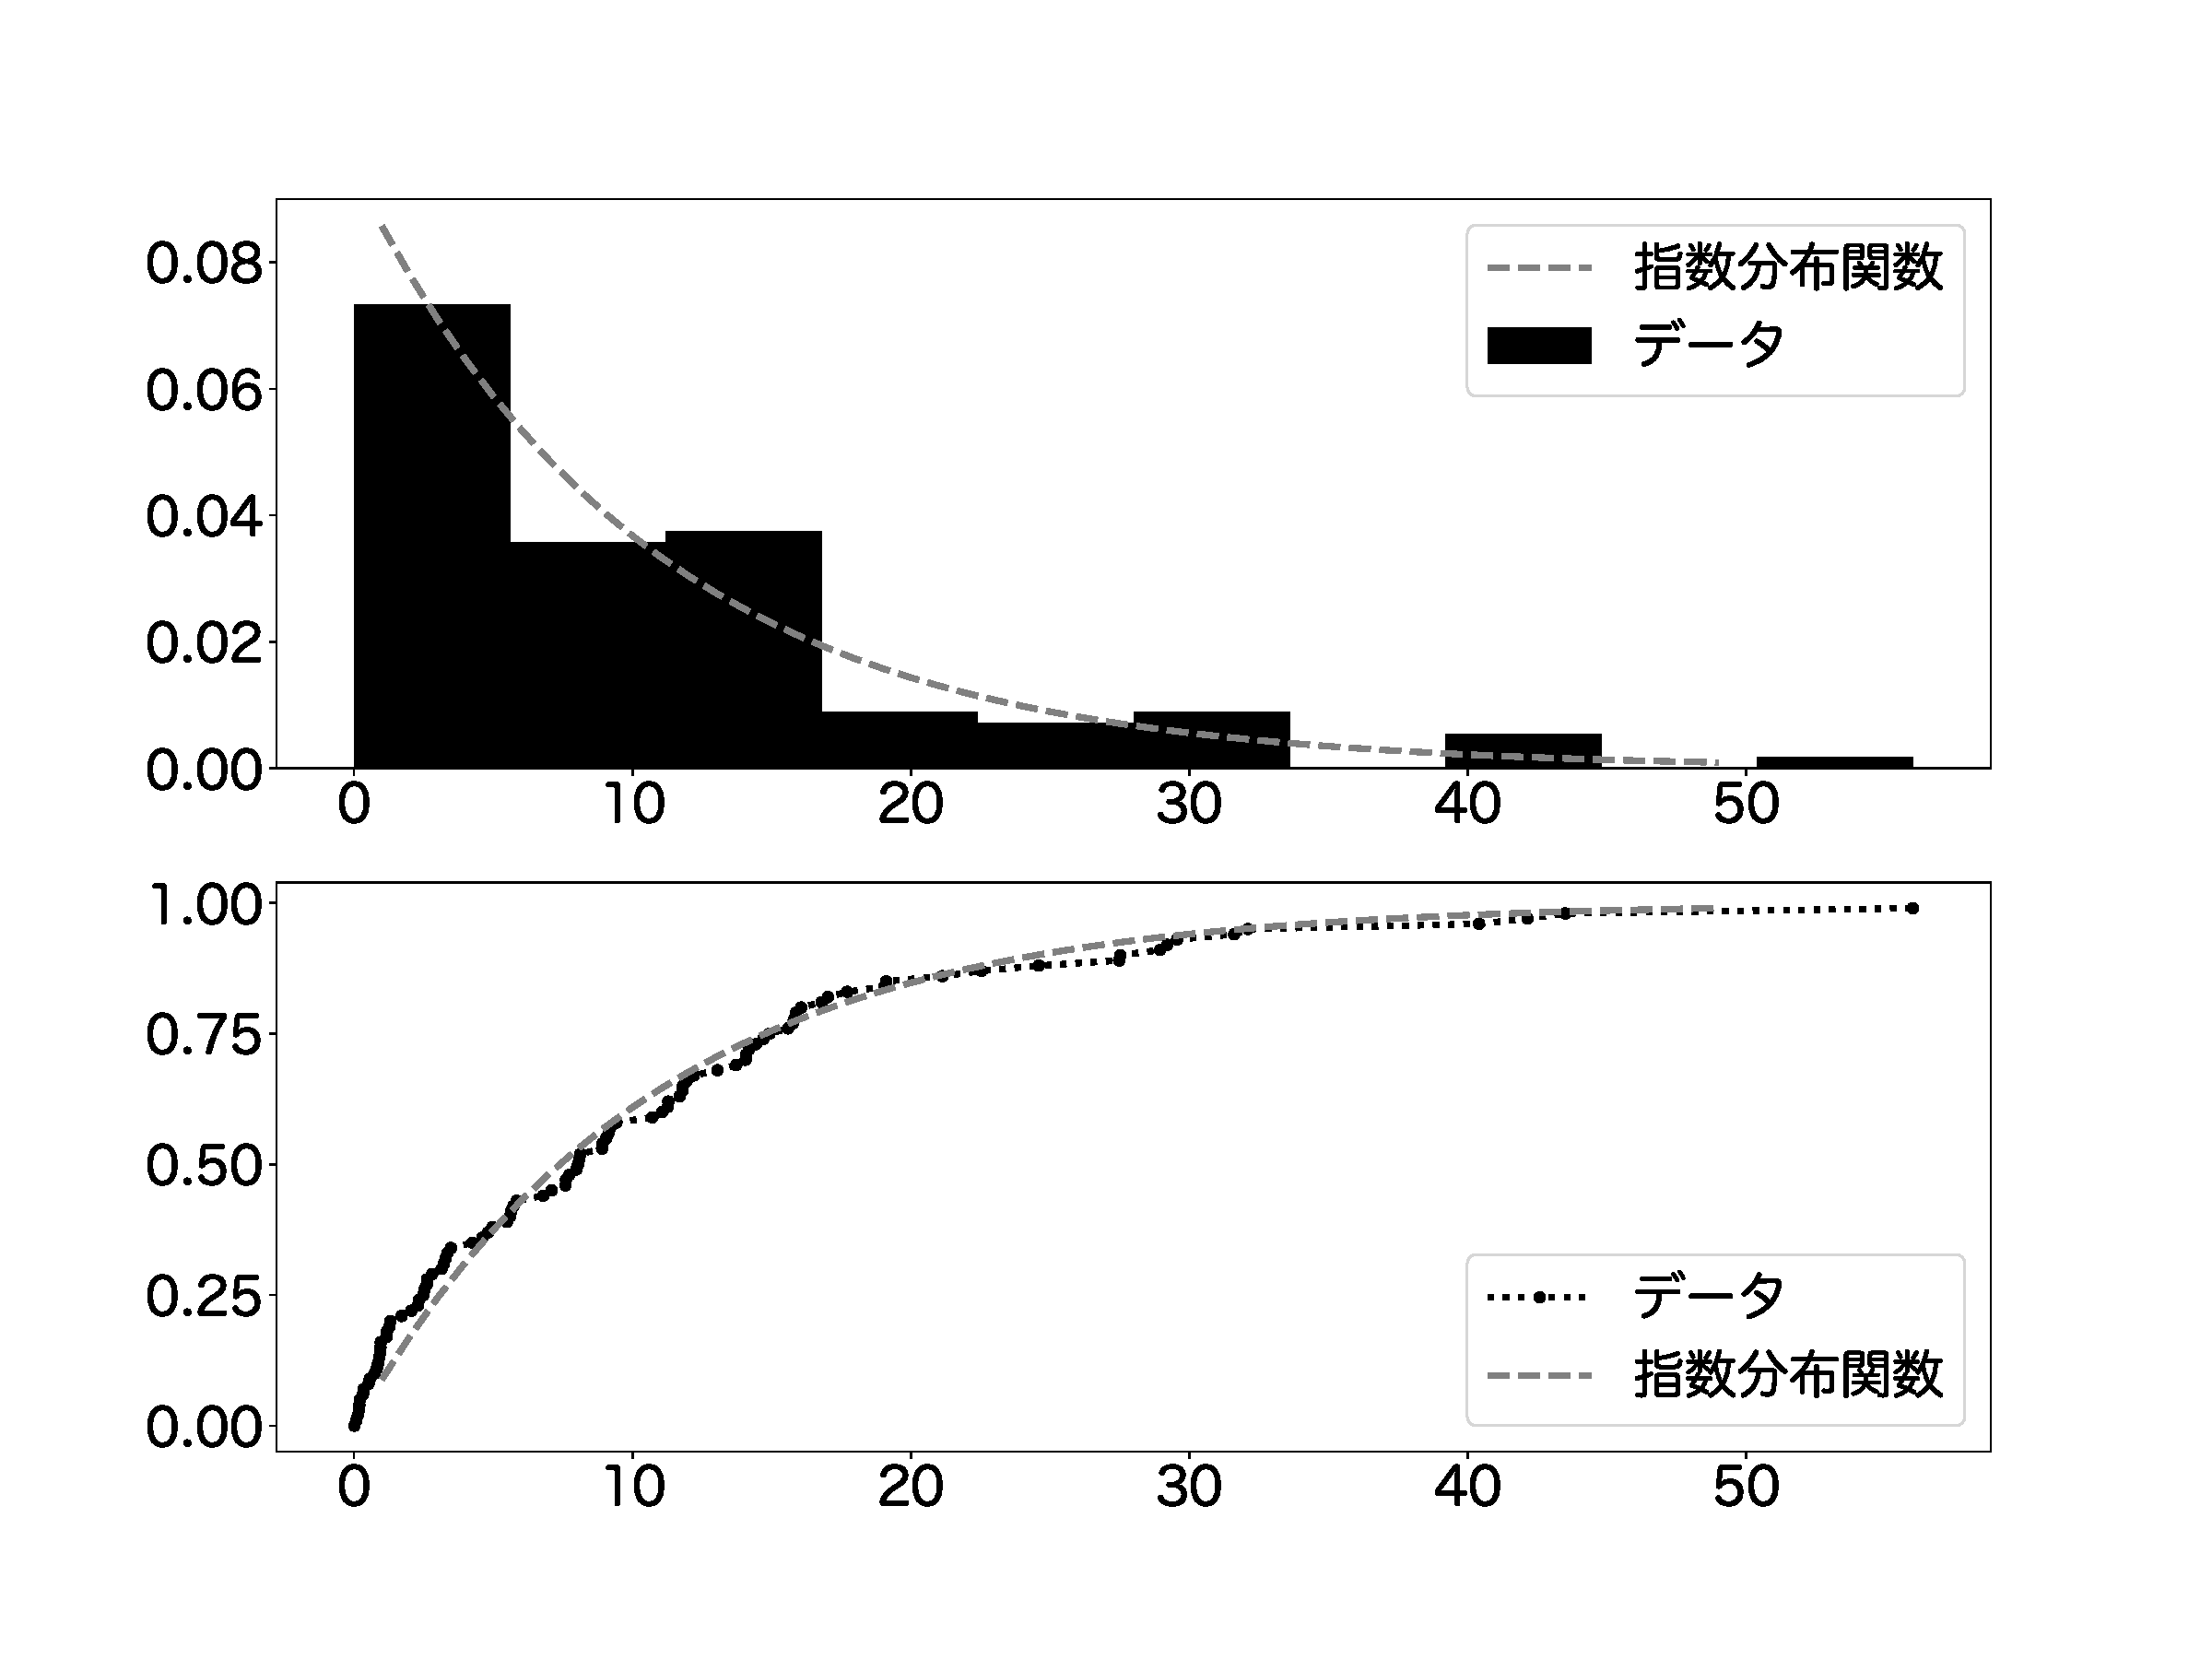
\includegraphics[width=15cm]{./image/06_/lambda_0.1.pdf}
    %\caption{しばらくした後の故障頻度の分布図}
\end{center}
\end{figure}





以上を通じて、単純に正規分布を仮定したモデルを導入すれば良し!とは言えないことがわかっただろう。言い換えれば、サンプルサイズが増えたときに見えてくる分布関数から母集団の構造を想定し、統計モデルを構築するべきだという方針が理解できる。
また、データの構造を理解した上で、推測を行うことで、データと推測が程よく一致することがわかった。


% https://biolab.sakura.ne.jp/small-sample-t-test-glm.html
\if 0
AICでモデルを選ぶと、正規分布の仮定がある。指数関数に対しては選択できないのでは? 
\fi
% https://eprints.lib.hokudai.ac.jp/dspace/bitstream/2115/49477/6/kubostat2008e.pdf
% http://www.ieice-hbkb.org/files/01/01gun_12hen_01.pdf




\paragraph{AAA}
あるとき、「改良することで故障日が伸びたみたいなんだ。調査してくれ」と依頼された。サンプルサイズは10程度であり、以下のようになった(今回も指数分布を使ってデータを生成した。もちろん実際の現象は数学の関数で生成されているわけではない)。

\begin{lstlisting}
6.46239039  7.5235678  31.84227772  6.73334029  2.9221049   1.84776618  8.7189158   2.97501827 57.78271493 20.51976339
\end{lstlisting}

統計モデルを構築しよう。
\begin{quote}
    \begin{enumerate}[(1)]
\item i.i.d
\item 正規分布
\item $\mu=10$
\end{enumerate}
\end{quote}

とする。以前のデータ解析では、指数関数を利用し、その平均値は10程度であった。今回の統計モデルでは平均$10$の正規分布を利用することで、この統計モデルが棄却できるかを試してみよう。



\begin{lstlisting}
stats.ttest_1samp(Y, 10)
\end{lstlisting}




その結果、$p=0.421$であることがわかった。このことから、有意水準$p<0.05$を満たしていないので、帰無仮説は棄却で聞いないので、改良できていないという判断を行うべきだろうか?
もちろん良くない。モデルの仮定をみると、統計モデルの仮定(2)が正規分布になっている。これは、我々が扱っている標本にはうまく適応できないことが経験的に理解してきた。
では、次のモデルはどうでしょう。

\begin{quote}
    \begin{enumerate}[(1)]
\item i.i.d
\item 指数分布
\item 指数分布の母数$\lambda=0.1$
\end{enumerate}
\end{quote}
このモデルは、故障日をよく予測してくれることがわかっている。
今回、統計モデルが正規分布ではないので、これまでの仮説検定により、統計モデルとデータの乖離を評価できない。そこで、数理統計学の知識を使う。

\subsection{指数分布関数の仮説検定}
確率変数$X_1,X_2,\cdots,X_n \sim i.i.d \ Exp(\lambda)$は、$n\bar{X}\sim Ga(1,\frac{1}{\lambda}) $ただし、$\bar{X}=X_1+X_2 \cdots +X_n$ここで、$Ga(1,\lambda)$は、尺度母数$\lambda$のガンマ分布である。統計量$\bar{X}$を利用した検定ができることが示唆される。
%https://ds.machijun.net/clear-exercise-of-statistics/%E7%AC%AC7%E7%AB%A0-%E6%8C%87%E6%95%B0%E6%AF%8D%E9%9B%86%E5%9B%A3ex%CE%BC%EF%BC%89%E3%81%AE%E6%AF%8D%E5%B9%B3%E5%9D%87%E3%81%AE%E4%BF%A1%E9%A0%BC%E5%8C%BA%E9%96%93%E3%81%A8%E6%A4%9C%E5%AE%9Ap128/



\subsection{尤度比検定}
TODO: 尤度比検定の定義

我々のデータをもとに推論をすると、
$$
\eta= \frac{\lambda_0\exp\left({-\lambda_0\sum x_i}\right)}{\bar{\lambda}^n \exp{(-n)}}
$$
ここで、$\bar{\lambda}$は最尤推定量であり、$\frac{n}{\sum x_i}$、$\lambda_0=0.1$,$n$はサンプルサイズである。
以上を元に、$\eta$を計算する。
$$
-2\log \eta \sim \chi^2_1
$$

より、$p=0.1902$と計算できる。$p$値を計算したら、やることはいつも同じで、統計モデルの仮定をもう一度調べる。統計モデルの仮定(1)はおそらく問題ない。統計モデルの仮定(2)は、少しの改良を加えただけなので、母集団の特性はほとんど変わっていなと前提を置いているので、悪くない近似ができることを期待している。統計モデルの仮定(3)は、$\lambda=0.1$である。$p>0.05$より現状では母数$\lambda$が変化しているとは言い切れない。




\begin{lstlisting}
9.70693386 14.74490149 33.03244855 21.8343649  40.73749837
\end{lstlisting}


さらにサンプルサイズが増えた。この場合、$p=0.01325$となり、$p=0.05$の有意水準を満たす。$N$数をどこまで増やすべきだったのだろうか。

TODO いつかかくけど、どこまで増やすんだろうか。
理想的には構造がわかるまで計測できたら嬉しい



\subsection{分散分析}
Section.2で行った分析では、様々な母平均に対して、統計モデルの推定がデータと一致することを確かめた。今回は、ばらつきを変化させ、統計モデルと推定の一致について考えてみよう。
統計モデルを構築しよう。
\begin{quote}
    \begin{enumerate}[(1)]
\item i.i.d
\item 正規分布$N(170,\sigma^2)$
\item 正規分布の母数$\sigma$
\end{enumerate}
\end{quote}
このモデルを、$M(\sigma)$とする。身長を予測するモデルとして、分散を替えてみよう。
Section.2で利用していた$M(5.7)$に対して、$M(10.0)$が現象を推定可能かを検討してみよう。
分布関数を書いてみると、グラフの裾野が広がったことが見て取れる。その分、ピークである$170$のあたりの頻度が減少している。つまり、$170$が出てくる頻度が下がり、より様々な身長の人がサンプリングできることが期待される。一方で、$M(2.0)$では、$170$の辺りが増え、他の場所では、頻度が現象することがわかる。$M(5.7)$よりも、身長のバラエティが少ないデータにたいし適合できる。


\begin{lstlisting}
163.54258776 179.15834405 172.6934295  166.29185695 177.65182141 165.87491547 172.08610141 158.30711988 163.74574501 176.47887419
\end{lstlisting}




拒否するべき統計モデルはどのような母数をもつだろうか。
10人から無作為抽出したデータに対して、統計モデル$M(3.1),M(12.0)$は十分データを説明できるだろうか?
統計モデルの上で、確率変数$X_1,X_2,\cdots,X_n$から計量される以下の統計量を定義する。
$$
Y_0=(n-1)\left(\frac{S_x}{\sigma}\right)^2
$$
ここで、$S_x^2=\frac{1}{n-1}\sum_{i=0}^{n}(x_i-\bar{x})^2,\bar{x}=\frac{1}{n}\sum_{i=0}^{n}x_i$である。
統計量$Y_0$は、$Y_0\sim\chi^2_{n-1}$であることがわかっている(定理\ref{fig:normal_sigma_chi2})。
このとき、$M(3.1),M(12.0)$については、$p<0.05$となり棄却される。
$p$値を基準にして、絶対にだめな統計モデル$M(3.1)$から、サンプリングを行ってみる。
\begin{lstlisting}

165.02227239, 163.16327065, 170.40109545, 170.81675656, 167.80872784, 166.91030856, 167.24096441, 170.44877048, 165.99400494, 167.59131488
\end{lstlisting}

統計モデル$M(5.7)$よりも値が広がった印象があると直ちにはわからない。
$M(3.1)$を使って、$180cm$を超える人の割合を計算すると、$P(X>180)<10^-5$となり、観測と比較してかなり少ない。
同様に、統計モデル$M(12.0)$を使って計算を行うと、$P(X>180)=0.15$となり、観測と比べて多いこともわかる。
棄却されなかった統計モデル$3.1<\sigma<12.0$の中でも、積極的に予測に利用するには、データの構造をより理解する必要がある。


\begin{figure}
\begin{center}
    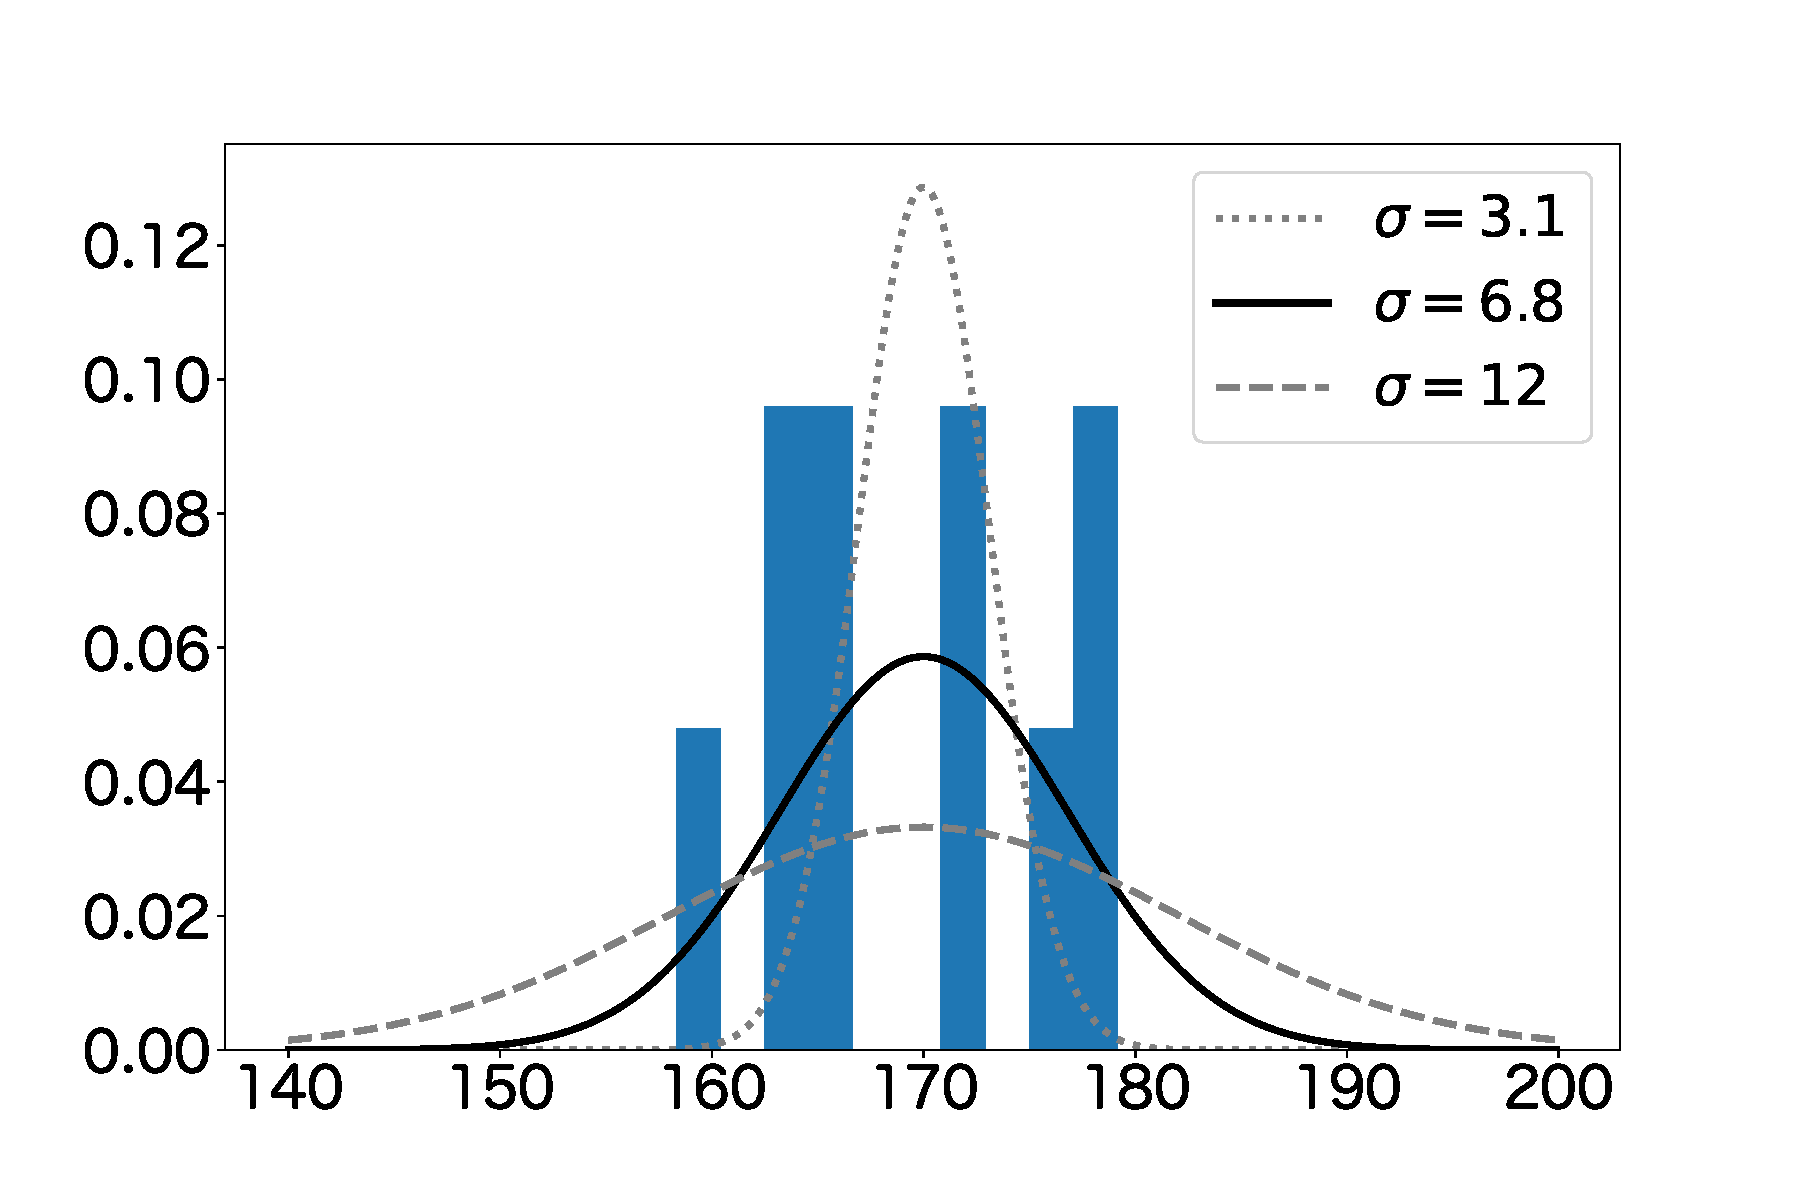
\includegraphics[width=15cm]{./image/06_/normal_sigma.pdf}
    %\caption{検出力}
\end{center}
\end{figure}

\if 0
https://biolab.sakura.ne.jp/welch-test.html
https://biolab.sakura.ne.jp/welch-anova-statwing.html
https://biolab.sakura.ne.jp/welch-test.html
\fi



%
\chapter{誤差論}
%\footnote{以下の論文を読んでの意見である\cite{Error_bar_nature,krzywinski2013importance}}
%真である理論値へ実験が近づけたことを検証することを目的にしており、理論に重点をおき、計測を疑うという点で生物学などのデータ解析とは異なる。
誤差論は、計測に対する信頼性を定量的に扱う方法論である。
計測に利用する計測機は、計測を行えば誤差を伴う。その誤差は以下の誤差の公理を満たすものとする。
\begin{enumerate}
    \item 誤差には中心がある。中心を対象に同等にデータが生じる。
    \item 絶対値の小さい誤差の方が大きな誤差よりも現れる頻度が高い
    \item ある程度以上の大きな誤差は生じない
\end{enumerate}


\section{標準偏差か標準誤差か}
%標準偏差や標準誤差によりデータのばらつきを捉えようとすることは、正規分布を含んだモデルを使って、母集団を推測しようとする行為であると考えることができます。以下の議論は、モデルが現象をよく捉えている場合にはうまく成り立つが、そうでないなら、モデルを修正したほうが、うまく現象をうまく捉えることができる\footnote{様々な意見がある\cite{SUZUKI_SESD,池田郁男2013統計検定を理解せずに使っている人のために,池田郁男2019改訂増補版}}。
%ここでは、次のモデル$M(\mu,\sigma^2)$を使う。
\if 0
\begin{enumerate}
    \item i.i.d
    \item 正規分布関数
    \item $\mu,\sigma^2$
\end{enumerate}

ここで、母集団から無作為抽出した標本の標本平均と標本分散をそれぞれ、$\bar{x}=\frac{1}{n}\sum{x_i},s^2=\frac{1}{n}\sum(x_i-\bar{x})^2$である。これらを組み入れた統計モデルを$M(\bar{X},s^2)$と書く。
\fi

\subsection{標準偏差}
正規分布を含んだ統計モデルを仮定し、そのモデルの上で、予想されるサンプルがおよそ$68\%$の確率で出現する範囲は、母数分散$\sigma^2$より以下の範囲になります。
\begin{equation*}
    [\mu-\sigma,\mu+\sigma].
\end{equation*}
モデルの母数分散は不明な場合、母集団から無作為抽出を行なって集計した標本の偏差$s$を計算します。
\begin{equation*}
    s = \sqrt{\frac{1}{n}\sum(x_i-\bar{x})^2}.
\end{equation*}
このことから、モデルが予測するサンプルが$68\%$の確率で出現する範囲は
\begin{equation*}
    [\mu-s,\mu+s].
\end{equation*}
これを図示したものが、図です。
言い換えれば、これは、$68\%$予測区間である。


\begin{figure}
    \begin{center}
        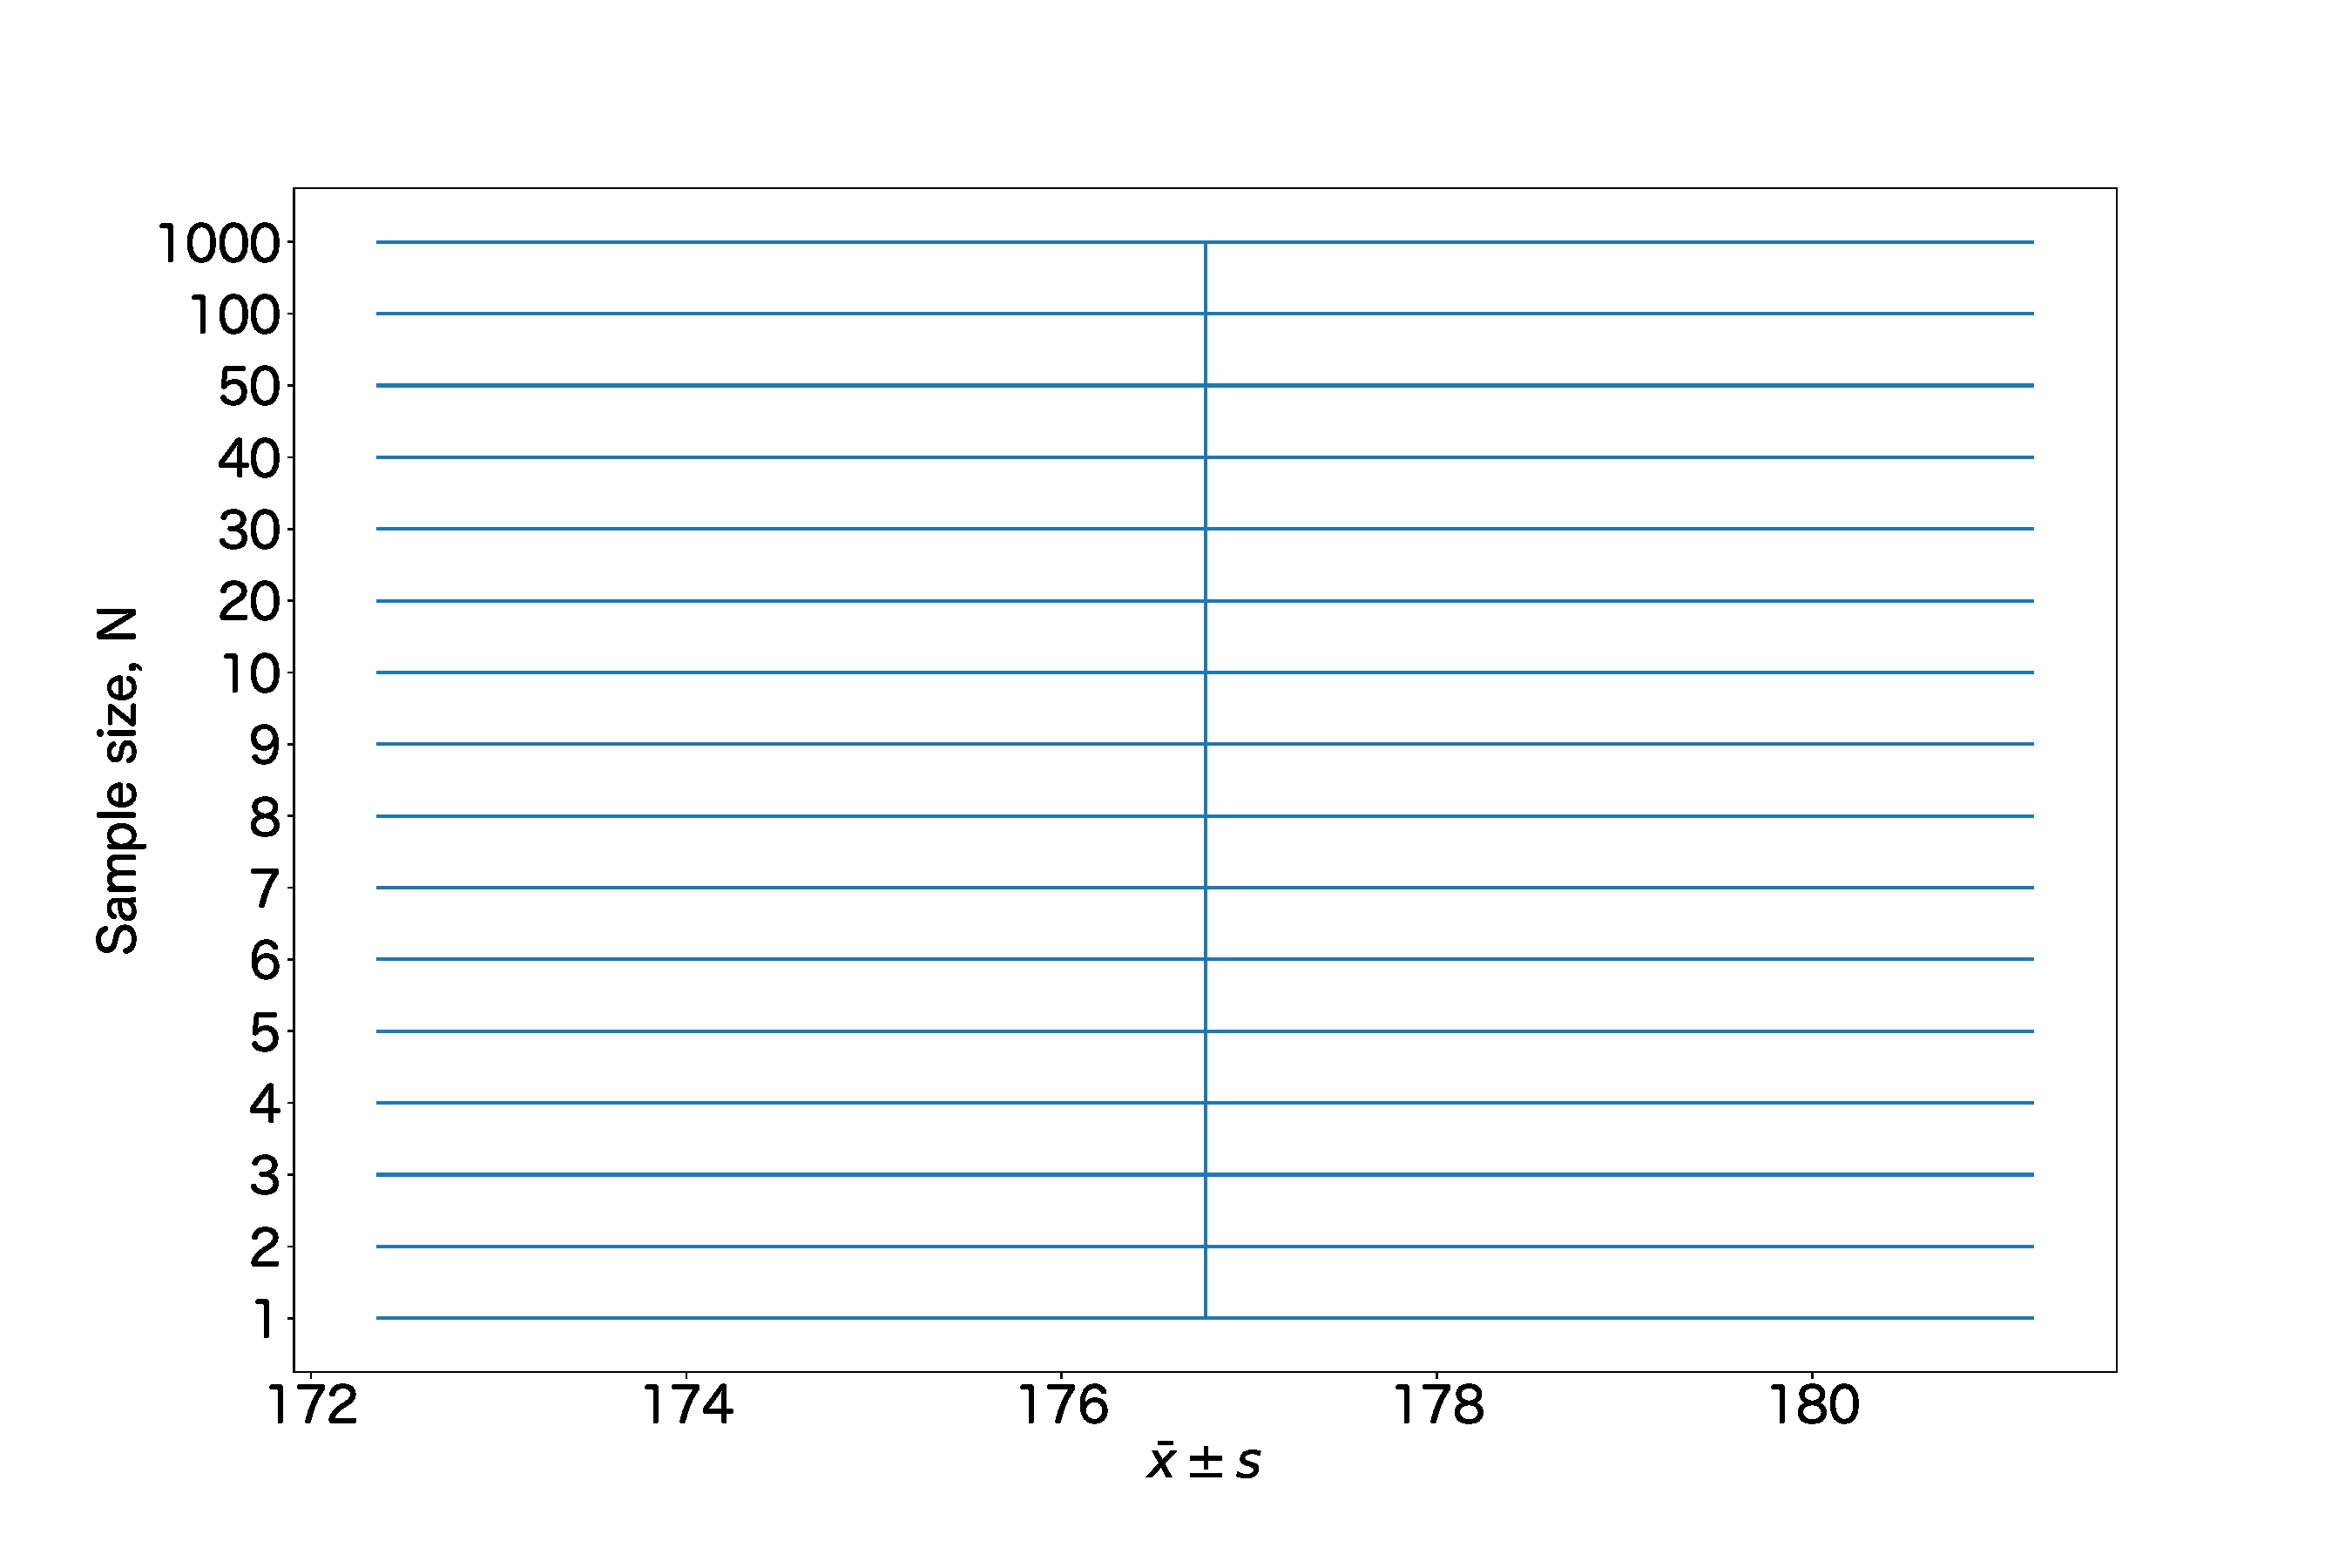
\includegraphics[width=15cm]{./image/10_/Norm_standard_deviation.pdf}
        \caption{サンプルサイズに応じた標準誤差の広がり}
        %\label{fig:standard_normal_distribution}
    \end{center}
\end{figure}



\subsection{標準誤差}
標準誤差$SE$は、標準偏差$s$をサンプルサイズ$N$の平方根で割ったものである。
\begin{equation*}
    SE = \frac{s}{\sqrt{N}}
\end{equation*}
$\bar{x}\sim N(\mu,\sigma^2/\sqrt(N))$であるので、モデルの上で$\bar{x}$が以下の範囲に出現する確率は、およそ$68.2\%$である。
\begin{equation*}
    [\bar{\mu}-SE,\bar{\mu}+SE]
\end{equation*}
よって、$\mu$の値は一般にわからないので、標本平均$\bar{X}$を用いて、
\begin{equation*}
    [\bar{X}-SE,\bar{X}+SE]
\end{equation*}
である。
統計モデル$M(\bar{x},s^2)$からサンプリングした$\bar{X}$がこの範囲に得られる確率が$68.2\%$である\footnote{$\sigma$が変曲点であるから使ったと思われるが、なぜ、$68.2\%$または、$\bar{X}\pm SE$の範囲を使ったのかはわからなかった。誤差論の立場では、以下の記述が見つかった\cite{誤差の取り扱い_神戸大学}。
\begin{quote}
    したがって、おおよそ$70\%$の確率で誤差の絶対値は$\sigma$より小さいことがわかるので、これを測定値の信頼度の目安として用いる。
\end{quote}
}
\footnote{標準偏差に ± を付けるな!: 医療論文に多い?
\url{https://biolab.sakura.ne.jp/mean-sd.html}。まだ読めていない。$\pm SE$という表記はよろしくないらしい。}。
言い換えれば、$SE$は、$68\%$信頼区間である。


\begin{figure}
    \begin{center}
        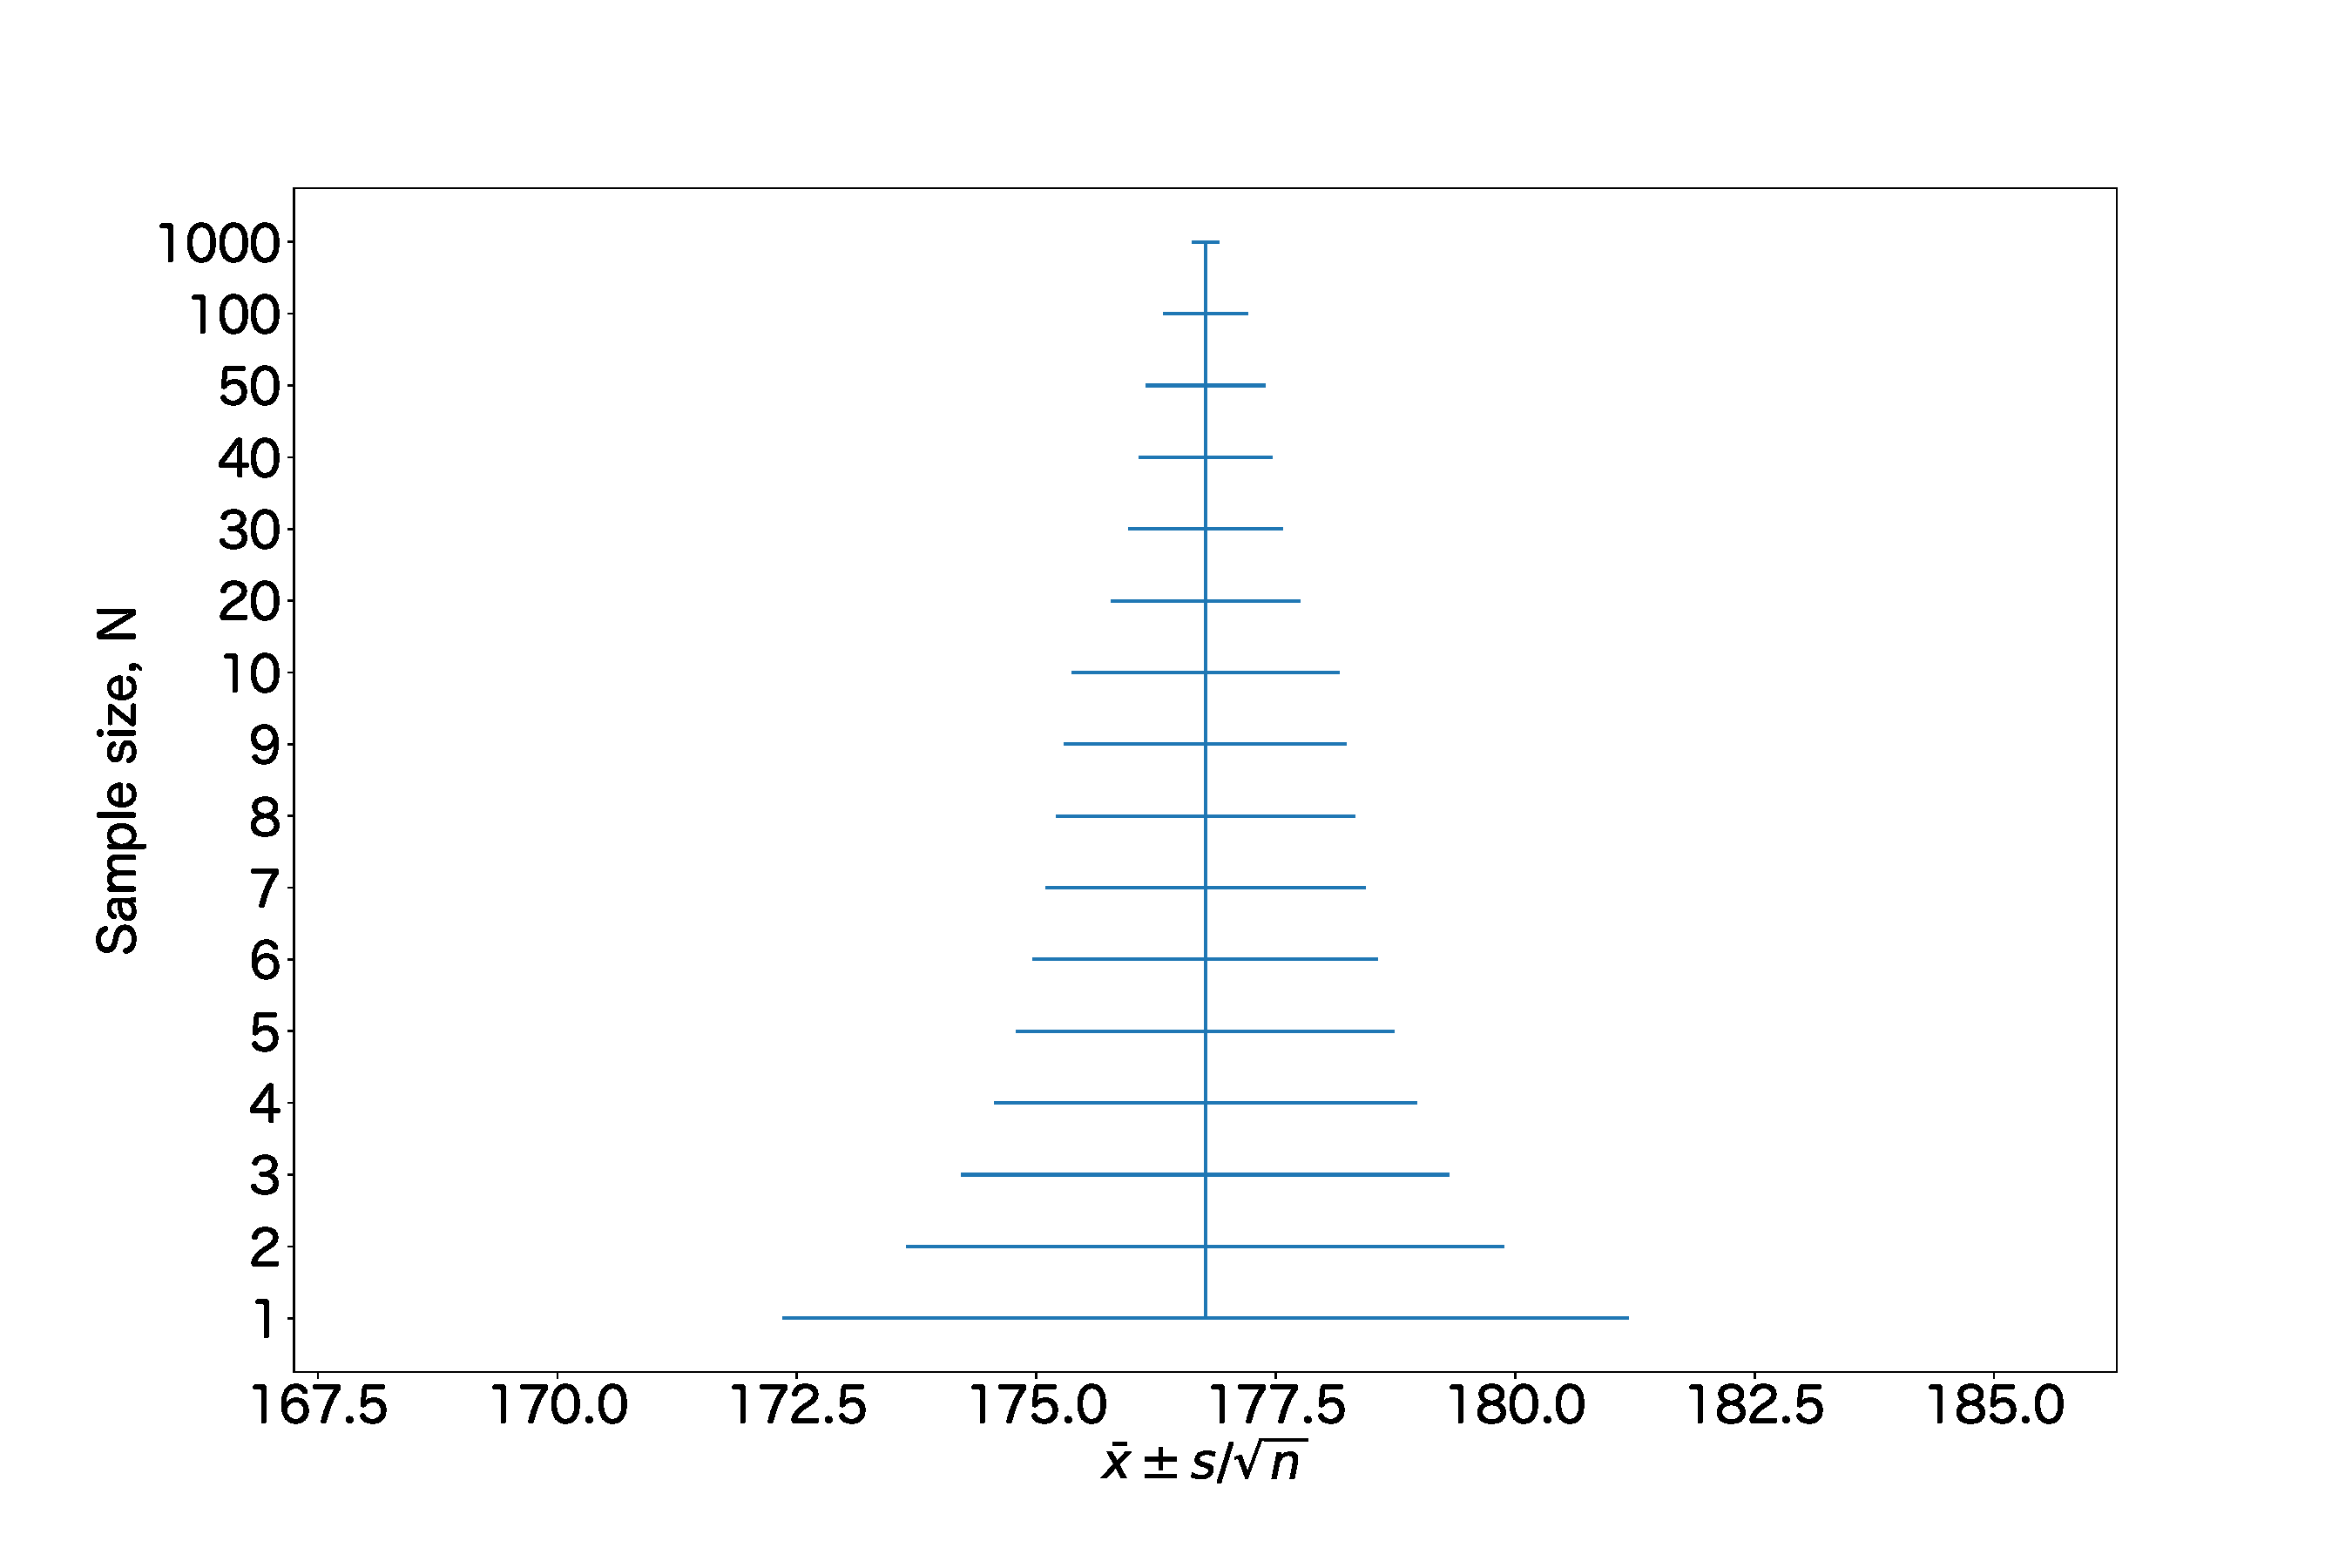
\includegraphics[width=15cm]{./image/10_/Norm_SE.pdf}
        \caption{サンプルサイズに応じた標準偏差の広がり}
        %\label{fig:standard_normal_distribution}
    \end{center}
\end{figure}




\chapter{統計モデル2}
ここでは、二つの確率変数から得られた確率変数についてその性質を議論する。

\section{正規分布二つを含んだ統計モデル}
次の3つを仮定したモデルを正規$2$モデルと呼ぶ。
\begin{quote}
    \begin{enumerate}[(1)]
    \item $x_i$および、$y_i$はそれぞれ独立同分布
    \item その分布は、正規分布
    \item 正規分布の母数はそれぞれ$\mu_1,\sigma_1^2,\mu_2,\sigma_2^2$とする。
    \end{enumerate}
\end{quote}
この正規2モデルを$M(\mu_1,\mu_2,\sigma_1^2,\sigma_2^2)$と書く。$\sigma_1,\sigma_2$を特定の値に設定したモデルを$M(\mu_1,\mu_2)$または、$M(\mu_1,\mu_2;\sigma^2_1,\sigma^2_2)$とし、$\mu_1,\mu_2$を特定の値に設定したモデルを$M(\sigma_1^2,\sigma_2^2)$または$M(\sigma_1^2,\sigma_2^2;\mu_1,\mu_2)$とする。
データから最尤推定を行なった母数を持つモデル$M_{ML}=M(\mu_{1,ML},\mu_{2,ML},\sigma_{1,ML}^2,\sigma^2_{2,ML})$を最尤正規2モデルという。

\subsection{信頼区間}
統計モデル$M(\mu_1,\mu_2;\sigma^2,\sigma^2)$により、$x_1,x_2,\cdots,x_n$,$y_1,y_2,\cdots,y_m$とサンプリングされたとする。次の統計量を定義する、
$$
Z=((\bar{x}-\mu_1)-(\bar{y}-\mu_2))\frac{\sqrt{mn}}{\sigma\sqrt{m+n}}
$$
ただし、$\bar{x}=\frac{1}{n}\sum_{i=0}^{n} x_i,\bar{y}=\frac{1}{m}\sum_{i=0}^m y_i$である。
$Z$は、$Z\sim N(0,1)$となることがわかっている。

信頼区間は、$Z$の大きさ$|Z|$によって決まる。
$\alpha=0.05$とすると、
\begin{eqnarray*}
&|Z|& < z_{0.025}\\
&\rightarrow & |(\bar{x}-\mu_1)-(\bar{y}-\mu_2)|\frac{\sqrt{mn}}{\sigma\sqrt{m+n}} < z_{0.025}\\
&\rightarrow& |(\bar{x}-\mu_1)-(\bar{y}-\mu_2)| <z_{0.025}\frac{ \sigma\sqrt{m+n} }{ \sqrt{mn }}\\
\end{eqnarray*}
式を展開すると、
\begin{equation*}
    (\mu_1-\mu_2)-z_{0.025}\sigma\sqrt{\frac{1}{n_1}+\frac{1}{n_2}} \leq \bar{X}-\bar{Y} \leq (\mu_1-\mu_2)+z_{0.025}\sigma\sqrt{\frac{1}{n_1}+\frac{1}{n_2}}.
\end{equation*}
を得る。
統計モデル$M(\mu_1,\mu_2)$によるサンプリングによって得られた平均値の差の大きさは、右辺よりも小さくなることが、$95\%$くらいの確率でモデル内でおこる。
実際に、何度も統計モデルからサンプリングを行なってみると、$95\%$くらいの確率でこの等式が成り立っている。計算機で試してみる。
\begin{lstlisting}
mu1 = 10
mu2 = 10
sigma = 5
m=10
n=20

norm1 = norm(mu1,sigma)
norm2 = norm(mu2,sigma)

sample1 = norm1.rvs(size=(m,1000))
sample2 = norm2.rvs(size=(n,1000))

xbar1 = np.average(sample1,axis=0)
xbar2 = np.average(sample2,axis=0)
A = np.abs(xbar1-xbar2) < norm(0,1).interval(1-0.05)[1]*sigma*np.sqrt(m+n)/np.sqrt(m*n)
len(np.where(A==True)[0])
\end{lstlisting}
およそ950程度の標本で、不等式が成立していることが確かめられる。

計算機で計算するには、次のコードが使える。
\begin{lstlisting}
def tTest(X,Y,sigma):
    x_bar,y_bar = np.average(X),np.average(Y)
    M,N = len(X),len(Y)
    Z = (x_bar-y_bar)*np.sqrt(M*N)/(sigma*np.sqrt(M+N))
    p=norm.cdf(Z,0,1)
    return 1-p
tTest(X,Y,5.7)
\end{lstlisting}


\begin{lstlisting}
def rejectRange(X,Y,sigma):
    M,N = len(X),len(Y)
    Z = sigma*(np.sqrt(M+N))/np.sqrt(M*N)
    za,zb= norm.interval(0.95,0,1)
    return Z*za,Z*zb
rejectRange(X,Y,5.7)
\end{lstlisting}

%\subsection{信頼区間}
%平均母数$\mu_1,\mu_2(\mu_1\neq \mu_2)$のときに、

$Z$の不等式を変形していくと、次がわかる
\begin{equation*}
    (\bar{X}-\bar{Y})-z_{0.025}\sigma\sqrt{\frac{1}{n_1}+\frac{1}{n_2}} \leq \mu_1-\mu_2 \leq (\bar{X}-\bar{Y})+z_{0.025}\sigma\sqrt{\frac{1}{n_1}+\frac{1}{n_2}}.
\end{equation*}
この式の意味は、何だっけ???TODO
%これは、$\bar{X},\bar{Y}$を得たときに、%$\mu_1-\mu_2$がこの範囲にあれば、$\mu_1=\mu_2$という統計モデルは棄却できない。



\subsection{検出力}
%二つの統計モデル$M(\mu,\mu),M(\mu_1,\mu_2)$において、を元に、検出力を計算する。
$M(\mu,\mu;\sigma^2,\sigma^2)$における統計量$Z$が、もう一つの統計モデル$M(\mu_1,\mu_2)$においての出現頻度を計算する。これは1標本のモデルと同様に検出力という。

$M(\mu,\mu)$において、
\begin{equation*}
    \frac{\bar{x}-\bar{y}}{U} \sim N(0,1)
\end{equation*}
である。ここで、$U=\sigma\frac{\sqrt{m+n}}{\sqrt{mn}}$である。
また、$M(\mu_1,\mu_2)$において、
\begin{equation*}
    \frac{\bar{x}-\bar{y}}{U}\sim N(\frac{\mu_1-\mu_2}{U},1)
\end{equation*}
である。上式の信頼区間$-z_{\alpha/2}\sim z_{\alpha/2}$が下式において出現するのは、確率分布が平行移動しているので、その区間を$[A,B]$とすると、ぞれぞれ
\begin{eqnarray*}
    A = -z_{\alpha/2}+\frac{\mu_1-\mu_2}{U}\\
    B = z_{\alpha/2}+\frac{\mu_1-\mu_2}{U}
\end{eqnarray*}
である。この区間に統計量が出現する頻度は、
\begin{equation*}
    \beta = \varPhi(B)-\varPhi(A)
\end{equation*}
により計算できる。ここで、$\varPhi(x)$は、標準正規分布の累積分布関数である。

\subsection{$\sigma$が異なるモデルでの検出力}
信頼区間は、
\begin{equation*}
    -z_{\alpha/2} \leq \frac{\bar{x}-\bar{y}}{U} \leq z_{\alpha/2}
\end{equation*}
ここで、$U=\sqrt{\frac{\sigma^2_1}{n_1}+\frac{\sigma^2_2}{n_2}}$である。
また、$M(\mu_1,\mu_2)$における統計量を$Z$とすると、$Z = \frac{\bar{x}-\bar{y}}{U}\sim N(0,1)$であるので、$a \sim N(\mu_1-\mu_2,U^2)$ならば、
\begin{eqnarray*}
    A &=& \frac{(a-(\mu_1-\mu_2))}{U} \\
        &=& (\mu_1-\mu_2)/U-z_{\alpha/2}
\end{eqnarray*}
同様に、
\begin{eqnarray*}
    B &=& \frac{(b-(\mu_1-\mu_2))}{U} \\
        &=& (\mu_1-\mu_2)/U-z_{\alpha/2}
\end{eqnarray*}
よって、
\begin{equation*}
    \beta = \varPhi(B)-\varPhi(A)
\end{equation*}
である。



\section{母分散が未知のときの統計モデル}


\subsection{信頼区間}


%\section{統計的仮説検定の手順}



\subsection{分散未知の場合}
%[統計学 講義](http://www3.u-toyama.ac.jp/kkarato/2020/statistics/handout/Statistics[B]-2020-25-0722.pdf)






\if 0
\section{正規分布を含んだ統計モデル}
我々は普段、男女の身長をみているから男性と女性を同じ統計モデルを用いて推測することは、到底無理だと言える。だが、あえて統計モデルを一つ構築して、男女の身長について推測を試みる。
\begin{quote}
    \begin{enumerate}[(1)]
\item i.i.d
\item 正規分布
\item 正規分布母数$\mu,\sigma=5.7$
\end{enumerate}
\end{quote}
この統計モデルを$M(\mu)$とかく。データを元にして、標準偏差は男女の差がほとんどなく、$5.7$程度であった。男性に対して制度の良い推測を行えていた$M(170)$を使って、女性の身長について推測してみる。女性で、$170cm$以上はどのくらいの頻度で現れるのか、$P(x>170)=0.5$である。一方で、データでは、$0.0179$である。また、平均身長は、データでは$157.8cm$程度である。このことから、統計モデルとデータが乖離していることがわかる。

\fi
\if 0
このように、二つの標本が異なることがわかっている、データでは、同じ統計モデルで予測するとデータに一致しないことがわかる。
\fi

\if 0
以上は、サンプルサイズが十分に大きい場合の平均値と分散を知っているから一つの統計モデルを使って男と女の身長を推測することが難しいことを示唆した。


一方で、サンプルサイズが十分ではない、言い換えれば、分布の特徴が掴みにくい場合、2標本を一つの統計モデルで推測するとまずいことがわかるのだろうか?
男と女、それぞれ5人から計測を行った、上が男、下が女の標本である。
\begin{lstlisting}

[161.92083043 162.3764036  170.60849829 166.64996998 164.83863778]
[159.58195311 152.93245418 159.18632478 145.77567615 152.13809195]
\end{lstlisting}



数式を書き換えれば、$|\bar{x}-\bar{y}|$の大きさによって決まることがわかる。
無作為抽出したデータの平均値$\bar{X},\bar{Y}$の差の絶対値がこの範囲に収まらなければ、この統計モデルは、現実を捉えていないと判断され、棄却される。

無作為抽出されたデータを用いて検定にかけてみると、$p=0.004$となり、$p=0.05$よりも小さいことがわかった。
%統計モデルの仮説が妥当であることを確認する。仮定(1)は満たされるように無作為抽出を行い計測したので、問題ないと考える。仮定(2)については、サンプルサイズを大きくしたときに、正規分布による予測がよく当たることを知っているので、この仮説も大きく外れているとは言い切れない。最後に、仮説(3)が間違っていることが示唆される。
%以上によって、帰無仮説が棄却される。

\fi
\chapter{モデルを使った研究の進め方}


\section{アヤメ(iris)に関する推論}
公開されているアヤメのデータを使って、研究の進め方について検討する。
このアヤメのデータでは$3$種(setosa,versicolor,virginica)のがく片の幅、がく片の長さ、花弁の幅、花弁の長さのデータが記録されている。
データサイズは、150で、種によって$50$ずつ記録されている。Pythonのライブラリsklearnから簡単にデータを呼び出せる。
\begin{lstlisting}
from sklearn import datasets
iris = datasets.load_iris()
\end{lstlisting}

\subsection{アヤメのがく弁の幅を予測するモデル}
ここでは、アヤメという植物が見つかったときどのようにモデルを構築するかを考える。
アヤメについてその種が3種類の分類が行われる前で、1種類であると考える。
%我々が得ているのは、アヤメという植物のがく片の幅のデータ$150$個である。

我々は、がく弁の幅を予測するモデルを構築したい。
この目的を達成できるかはわからないが、一手目に行うのは、データに適合するモデルを探索することである。
データをみると、ある点を対称に同じくらいの数のデータがあることがわかる。
このことから、正規モデルが候補にあげられる。
データから平均と分散を求めると、$\bar{X}=3.05,\sigma=0.434$であった。
このことから、最尤正規モデルを構築する$M_a=M(3.05,\sigma^2=0.434^2)$である。
最尤正規モデルがデータに適合しているかをみる。
このモデルの予想では、$\mu$より大きいまたは小さいデータの個数は半数程度である。
また、$\mu-\sigma \sim \mu+\sigma$の中にあるデータは$68\%$程度である。
表\ref{table:all_spael_width_table}がデータが予測にあっているかを示している。
どちらの指標も予想に合っている。
また、$>\mu$と$\mu<$となるデータの個数の比率も$1$に近い$1.24$であった。
これはモデルがデータに適合していることを示している。
\begin{table}[h]
    \caption{aa}
    \label{table:all_spael_width_table}
    \centering
    \begin{tabular}{lccccccc}
        %\toprule
        \hline
        {} &  $<\mu$ &  $>\mu$ &  Data Size &  $<\mu$ Rate &  $>\mu$ Rate &  $<\mu/>\mu$ & $\mu-\sigma\sim\mu+\sigma$\\
        %\midrule
        \hline
        All    &    83 &    67 &        150 &       0.55 &       0.45 &       1.24 & 0.673\\
        %\bottomrule
        \hline
    \end{tabular}
\end{table}

\begin{figure}
    \begin{center}
        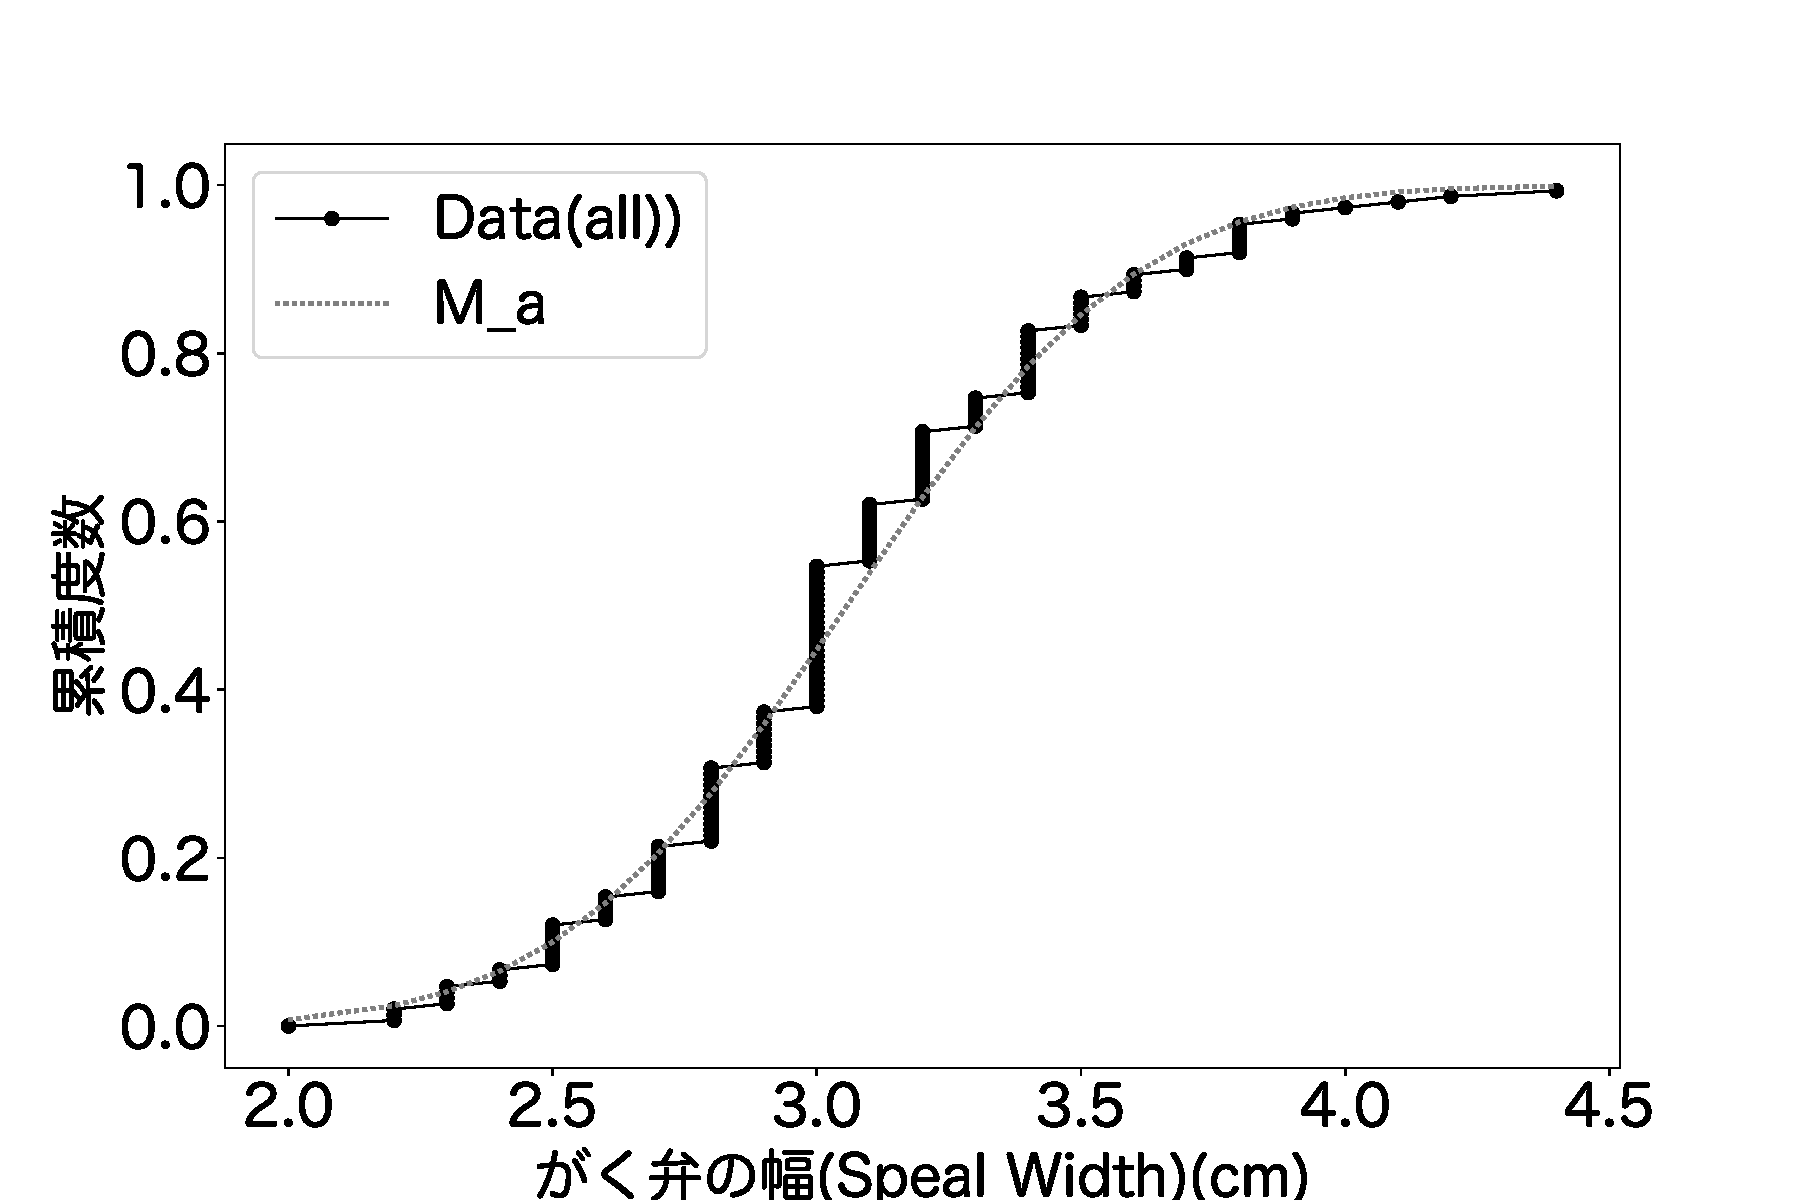
\includegraphics[width=15cm]{./image/15_/speal_width_all.pdf}
        \caption{データのがく弁の幅の累積度数(Data)と最尤モデルの累積度数$M_a$}
        \label{fig:all_speal_width_fig}
    \end{center}
\end{figure}

図\ref{fig:all_speal_width_fig}は、データの累積度数とモデルの累積度数を示している。
データとモデルの累積度数に関する予測がそれなりに一致していることがわかる。
このこともモデルがデータに適合していることを示唆している。

%アヤメについて統計モデルを使って予測する。
\subsection{アヤメの分類の細分化}
アヤメの分類を細分することになり、virginicaとそれ以外とすることになった。
これら二つのグループにおいて、がく弁の幅はこれまでに作ったモデル$M_a$により予測することができるだろうか。
新たにデータを取得し、モデルの予測とデータを比べることでモデル$M_a$の予測性能を測ることができる。
今回はデータを得るのが難しいので、もう一度同じデータを使い、モデルのデータに対する予測性能を測る\footnote{モデル構築に使ったデータを再び使うので、モデル$M_a$の予測の良さを測れていない}。
表\ref{table:speal_width_virig}がモデル$M_a$の予測に対する実際のデータの性質を示している。
virginicaとそれ以外はモデル$M_a$によって十分予測できていない。
モデル$M_a$の平均母数$\mu$より小さなものと大きなものの比が1より離れた値を取っている。
また、データの$68\%$が見つかるという予測をする区間には、$68\%$とはかけ離れた割合のデータが存在する。
図\ref{fig:virginica_speal_width_fig}には、モデル$M_a$とデータの累積度数を表示している。
モデル$M_a$の累積度数の上にデータの点がないことからも、モデルとデータが乖離していることが示唆される。
 

\begin{table}[h]
    \caption{アヤメ(virginicaとそれ以外)のがく弁の幅に関するデータの割合。モデル$M_a$の平均値を$\mu$としたとき、$\mu$より小さなデータの個数と割合($<\mu$、$<\mu$ Rate)。$\mu$より大きなデータの個数($>\mu$)と割合($>\mu$Rate)。$<\mu$と$>\mu$の割合。$\mu-\sigma\sim \mu+\sigma$の中にあるデータの個数($68\%$)と割合($68\%$Rate)。}
    \label{table:speal_width_virig}
    \centering
    \begin{tabular}{lrrrrrrrr}

        %\toprule
        \hline
        {} &  $<\mu$ &  $>\mu$ &  $<\mu$ Rate &  $>\mu$ Rate &  $<\mu/>\mu$ &  $68\%$ &  $68\%$Rate &  Data Size \\
        %\midrule
        \hline \hline
        virginica   &     8 &    42 &       0.16 &       0.84 &       0.19 &   27 &     0.54 &         50 \\
        others &    75 &    25 &       0.75 &       0.25 &       3.00 &   74 &     0.74 &        100 \\
        %All    &    83 &    67 &       0.55 &       0.45 &       1.24 &  101 &     0.67 &        150 \\
        %\bottomrule
        \hline
    \end{tabular}
\end{table}
    
\begin{figure}
    \begin{center}
        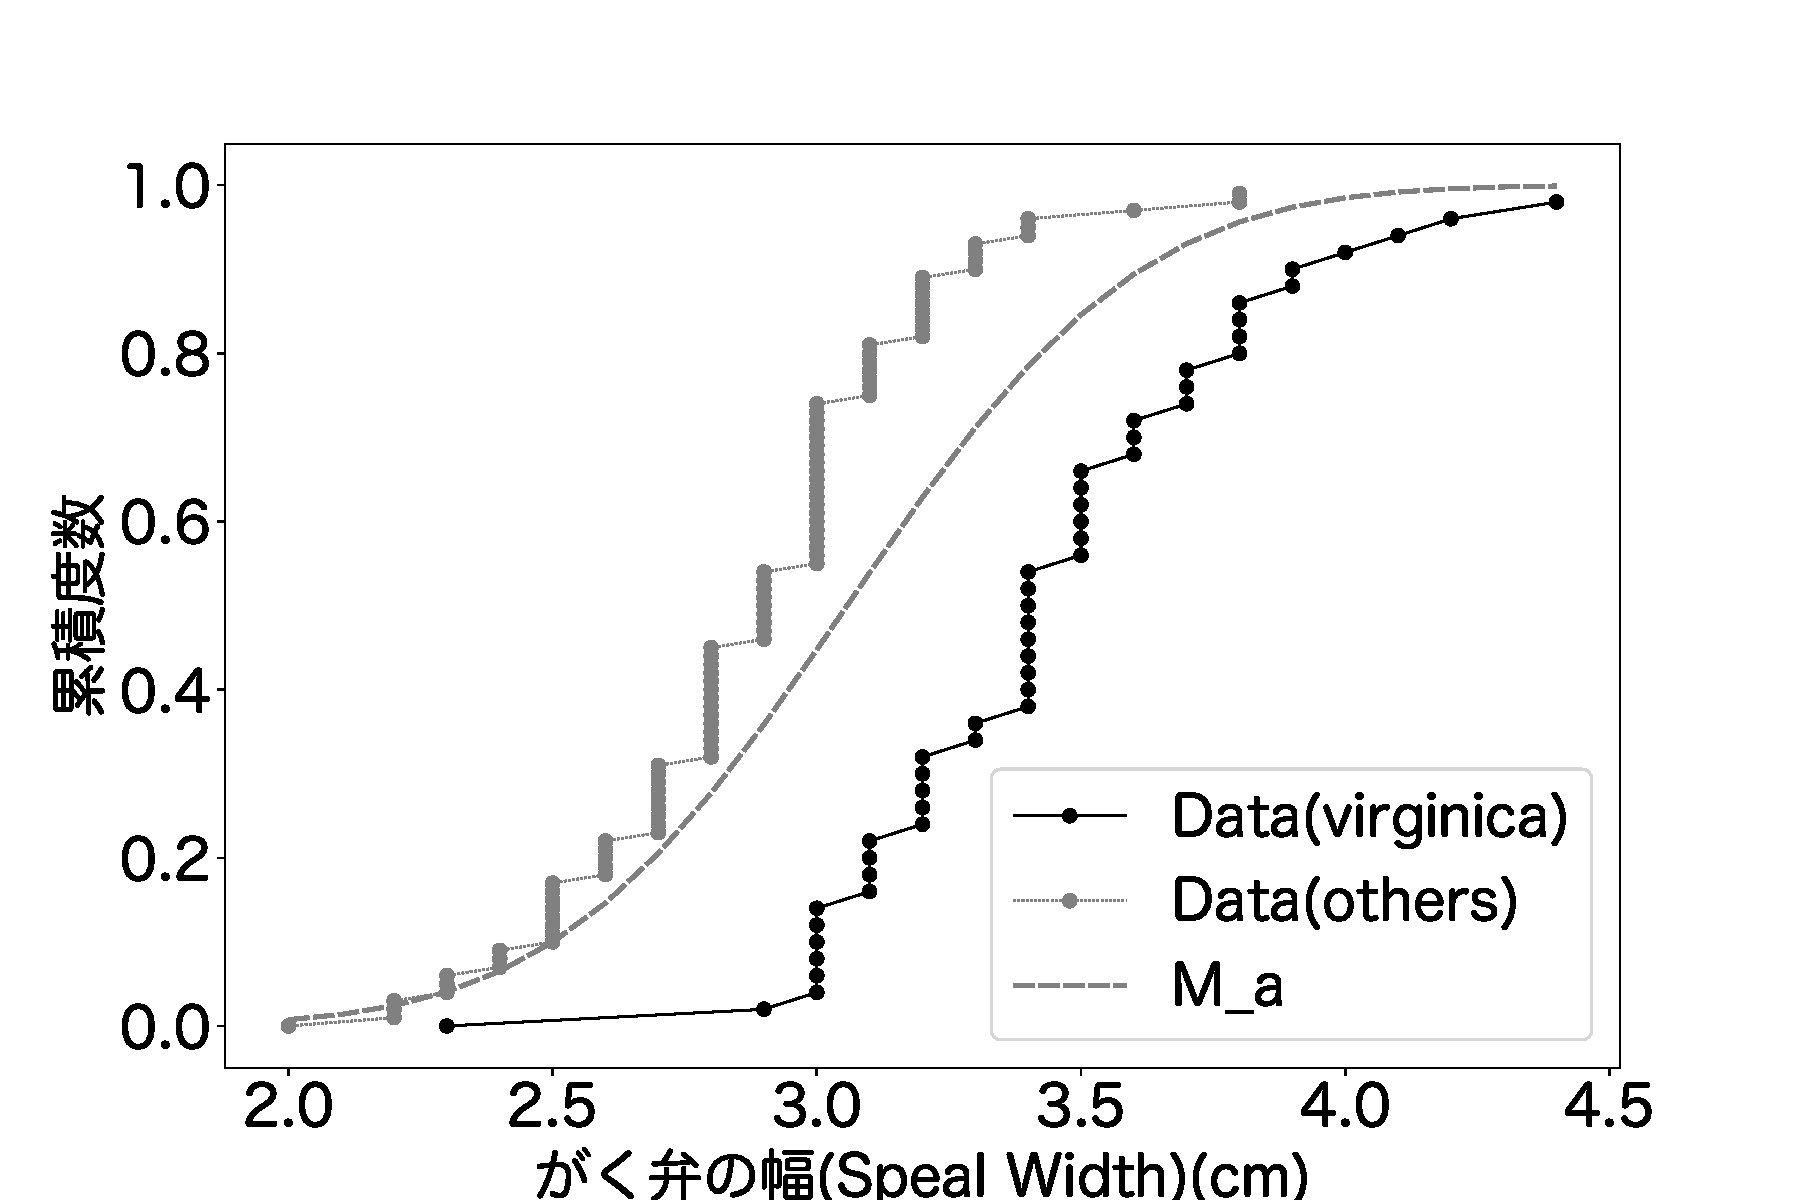
\includegraphics[width=15cm]{./image/15_/speal_width_viri.pdf}
        \caption{データのがく弁の幅の累積度数(Data)と最尤モデルの累積度数$M_a$}
        \label{fig:virginica_speal_width_fig}
    \end{center}
\end{figure}

モデル$M_a=M(\mu=3.05,\sigma^2=0.434^2)$における統計検定量も利用する。
次のことがわかっている。
\begin{equation*}
    Z = \frac{\sqrt{N}(\mu-\bar{x})}{\sigma} \sim N(0,1)
\end{equation*}
統計検定量$Z$を計算した結果が表\ref{table:speal_width_Z}である。
$Z$の絶対値は、$2$より大きくモデルとデータが乖離していることがわかる。

\begin{table}
    \caption{統計検定量$Z$}
    \label{table:speal_width_Z}
    \centering
    \begin{tabular}{lccc}
        \hline
        {} &   $\bar{x} $ &  $\sigma$  &     Z \\
        \hline \hline
        virginica &  3.43 &  0.38 & -6.03 \\
        others    &  2.87 &  0.33 &  4.27 \\
        $M_a$ & 3.05 & 0.434 & - \\
        \hline
    \end{tabular}
\end{table}

これらのことから、モデルの改訂をした方が良いことが示唆される。

以上のことは論文においては、統計統計量より偏った値が得られる確率($p$値)または$p<0.05$が報告される。
すでに議論した通り、$p$値だけでモデルとデータの乖離を検証すると、モデルの予測性能が過度に低いと判定されることがある。さまざまな指標を元にモデルの予測性能を測るべきである。

\subsection{新たなモデルの構築}
virginicaとothersに適合するモデルをそれぞれ構築する。
累積分布はどちらも正規分布的になっている。$M_a$を構築するときと同じようにそれぞれの平均と分散を求め(表\ref{table:speal_width_Z}の通りである)、データが平均に対して対称に分布していること、$\mu-\sigma\sim\mu+\sigma$の間にあるデータが$68\%$程度であるかを確かめる。

\begin{table}
    \caption{新たなモデル$M_v,M_o$による予測とデータの適合具合}
    \label{table:speal_width_replace_model}
    \begin{tabular}{lrrrrrrr}
        %\toprule
        \hline
        {} &  $<\mu$ &  $>\mu$ &  $<\mu$Rate &  $>\mu$Rate &  $<\mu/>\mu$  &  $68\%$Rate &  Sample Size \\
        %\midrule
        \hline \hline
        0 &   28 &   22 &     0.56 &     0.44 &      1.27 &     0.72 &           50 \\
        1 &   46 &   54 &     0.46 &     0.54 &      0.85 &     0.72 &          100 \\
        %\bottomrule
        \hline
    \end{tabular}
\end{table}   

表\ref{table:speal_width_replace_model}には、新たなモデル$M_v$および$M_o$の予測とデータの適合具合を示している。
どの指標もモデルの予想と一致しており、モデルがデータと適合していることを示唆している。

\begin{figure}
    \begin{center}
        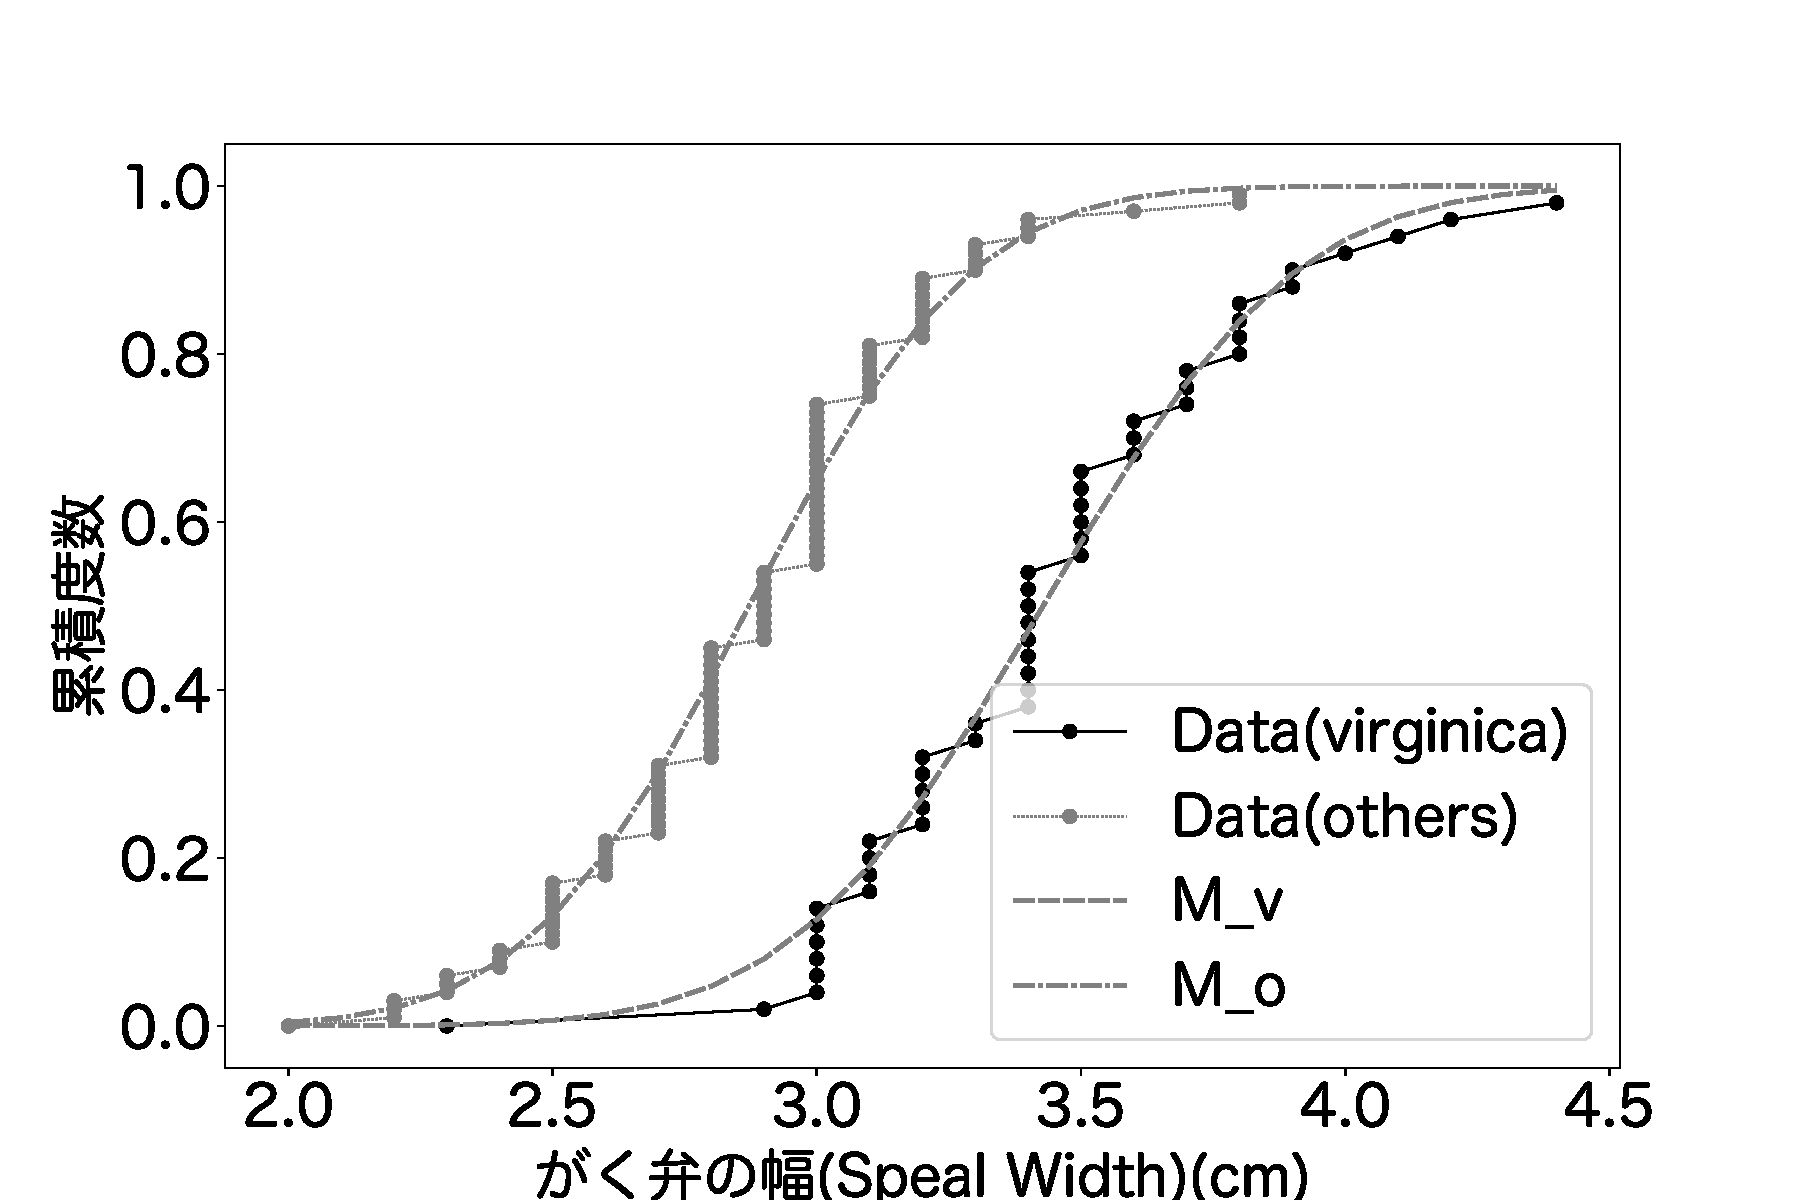
\includegraphics[width=15cm]{./image/15_/speal_width_viri_model.pdf}
        \caption{データのがく弁の幅の累積度数(Data)と最尤モデルの累積度数$M_v,M_o$}
        \label{fig:speal_width_viri_model}
    \end{center}
\end{figure}

図\ref{fig:speal_width_viri_model}はモデルの累積度数とデータの適合具合を示している。
それぞれのモデルがそれぞれデータをよく予測していることがわかる

\subsection{更なる細分化}
アヤメのothersについても細分化することになったsetosa,versicolorである。これらについて予測モデル$M_v$は良い予測をするかを調べ、予測できないと判断したのなら、モデルを構築し直すことになる。

%
\section{ノンパラメトリック検定}
\begin{mybox}
    \paragraph{正規分布じゃないからノンパラメトリック!}
    \begin{quote}
        サンプルサイズが大きい場合は、正規性の検定を行い、正規性でないと確認してからノンパラメトリック検定を使うと書いた文献もある\footnote{\url{https://katosei.jsbba.or.jp/view_html.php?aid=1196}.}。
        正規分布に近いとは言えないこともある場合、ノンパラメトリック検定を勧める文献もある \url{ http://j-ca.org/wp/wp-content/uploads/2016/04/5102_51kyo2_so.pdf . 臨床研究における統計学的解析 ─推定と検定の正しい使い方─}
        これらとは反対に、正規性検定をノンパラメトリック検定を利用するときの基準として使うべきでないと主張する論者もいる\footnote{https://biolab.sakura.ne.jp/normality-test-nonparametric.html}。
        ノンパラメトリック検定を勧められたときには、その検定の仮定を調べて、自分のデータと仮定が妥当であることが確認できるならば、ノンパラメトリック検定を使えば良い。
    \end{quote}
\end{mybox}

\subsubsection{Shapiro-Wilk検定}
Shapiro-Wilk検定で使う統計モデルは、次の二つの仮定により構成されている。
\begin{quote}
    \begin{enumerate}[(1)]
\item それぞれが独立に得られる
\item 正規分布
\end{enumerate}
\end{quote}
この検定を使うと、統計モデルの仮定(1)がクリアな場合、(2)が仮定できないと判断されます。つまり、$p$値が小さければ、正規分布ではないことが主張できます。一方で$p$値が大きい場合では、積極的に正規分布であるとは主張できません。

\begin{mybox}
    \begin{quotation}
t検定を使う前提条件としてShapiro-Wilk検定を使うことを推奨している文献があるようです。


統計モデルは真実ではありませんし、各仮定が前提である必要はありません。どのくらい正規分布から離れているかを判定するのは解析者に依存します。

統計モデルには、各変数が独立であることを仮定しますが、この仮定を前提にする統計的な手法の利用は推奨されてません。統計モデルの仮定のうち一つは前提としようと努力をするのですが、独立性については無視する立場があるのも確かです。我々は、統計モデルの仮定は本当に正しいことを要求しません。
\end{quotation}
\end{mybox}

% https://biolab.sakura.ne.jp/welch-anova-statwing.html

% http://ibis.t.u-tokyo.ac.jp/suzuki/lecture/2015/dataanalysis/L8.pdf
% https://biolab.sakura.ne.jp/normality-test-nonparametric.html




\subsubsection{ウィルコクソン(Wilcox)の符号順位検定}
ウィルコクソンの符号順位検定で使う統計モデルを構成する仮定は次の通りです
\begin{quote}
    \begin{enumerate}[(1)]
\item $i=0,\cdots,n$に対して、$Z_i=Y_i-X_i$とする。$Z_i$は互いに独立である。
\item $Z_i$は連続的母集団に従い、共通の中央値$\lambda$に関して対称である。
\end{enumerate}
\end{quote}  

% https://twitter.com/genkuroki/status/1444531128530976770
% https://www.jstage.jst.go.jp/article/psj/30/1/30_30.006/_pdf




\subsubsection{マン・ホイットニーのU検定}
\begin{quote}
    \begin{enumerate}[(1)]
\item 両標本が同じ分布関数から生成された(帰無仮説)
\item 等分散
\end{enumerate}
\end{quote}
ウィルコクソンの順位和検定
% https://ja.wikipedia.org/wiki/マン・ホイットニーのU検定
% https://oku.edu.mie-u.ac.jp/~okumura/stat/brunner-munzel.html



\subsubsection{対応ある t 検定}
1群の(差を作った)検定なので、等分散の仮定は必要ではない。中身が0と比べつ
% https://biolab.sakura.ne.jp/paired-t-test-two-sample-anova.html


\subsubsection{Walchの検定}
% https://biolab.sakura.ne.jp/maxima-welch-test.html
% https://oku.edu.mie-u.ac.jp/~okumura/stat/ttest.html


%
\appendix
\chapter{数理統計学}
データの出現頻度を近似する式である確率密度関数、累積分布関数について説明し、様々な形の確率密度関数について説明する。
さらに、特定の分布に従う確率変数が、その分布関数から生成された確率変数であることを確かめる方法について説明する。
最後に、モデルの確率変数への当てはまりの良さの相対的な指標である尤度を導入し、尤度を最大にする母数を推定する方法を説明する。
さらに、モデルのパラメータの数に対するペナルティを導入した指標のAICを導入する。

\subsection{確率密度関数}

\subsection{累積分布関数}
aaa

\subsection{相補累積分布関数}
$1$から累積度数を引いたものは、相補累積分布関数と呼ばれ、ある値よりも大きな値をえる確率示し、数式では、
\begin{eqnarray}
    1-F(x) &=& f(X>x) \\
        &=& \int_{x}^{\infty} f(z)dz.
\end{eqnarray}
図\ref{fig:standard_normal_distribution}(c)に図示した。累積分布関数と相補累積分布関数のどちらかを表示するかは、分野によって異なる\footnote{生物学の分野などでは、より大きな値を得る確率を重視することがあるので、累積分布関数よりも、相補累積分布関数が好まれることがあるように私は感じている。}。

\section{確率変数}
\subsection{確率変数がある分布関数に従う}
確率変数$x$が、ある分布関数に従うとは、

%$x$をたくさん集めて、$x_1,x_2,\cdots,x_n$という標本を得たときに、その出現頻度がその分布関数に精度よく近似できる。


\section{正規分布}
正規分布の確率密度関数は、
\begin{equation}
p(x;\mu,\sigma)=\frac{1}{\sqrt{2\pi\sigma^2}}\exp\left(-\frac{(x-\mu)^2}{2\sigma^2} \right)
\end{equation}
ここで、$\mu,\sigma^2$は、正規分布のパラメータで、それぞれ母数平均、母数分散です。
母数平均は最も出現頻度の高い数値を表しており、この値を中心にし、対象に分布が広がります。言い換えれば、$\mu-a$と、$\mu+a$の出る確率は同程度になります。
母数分散は、数値のまとまり具合を示します。$\sigma$が大きくなるほど、$\mu$の近くの数値が出現する頻度は小さくなり、より離れた場所での出現頻度を高くします。
正規分布関数に確率変数が従うことを$X\sim N(\mu,\sigma^2)$とかく。



正規分布においてその母数を$\mu=0,\sigma=1$とするとき、標準正規分布といい、$N(0,1)$で表す。確率変数$Z$が標準正規分布に従うとき、その確率密度関数は
\begin{equation}
\phi(z) = \frac{1}{\sqrt{2\pi}}\exp(-\frac{z^2}{2})
\end{equation}
であり、図\ref{fig:standard_normal_distribution}(a)である。
標準正規分布の累積分布関数は、
\begin{eqnarray}
\Phi(x) &=& p(X<x; 0,1) \\
    &=& \int_{-\infty}^x \phi(z)dz \\
    &=& \frac{1}{2}(1+\rm{erf}\frac{x-\mu}{\sqrt{2\sigma^2}})
\end{eqnarray}
であり、図\ref{fig:standard_normal_distribution}(b)である。

相補累積分布関数は、
\begin{eqnarray}
    1-\Phi(x) &=& p(X>x; 0,1) \\
        &=& \int_{x}^{\infty} \phi(z)dz.
\end{eqnarray}


\begin{figure}
    \begin{center}
        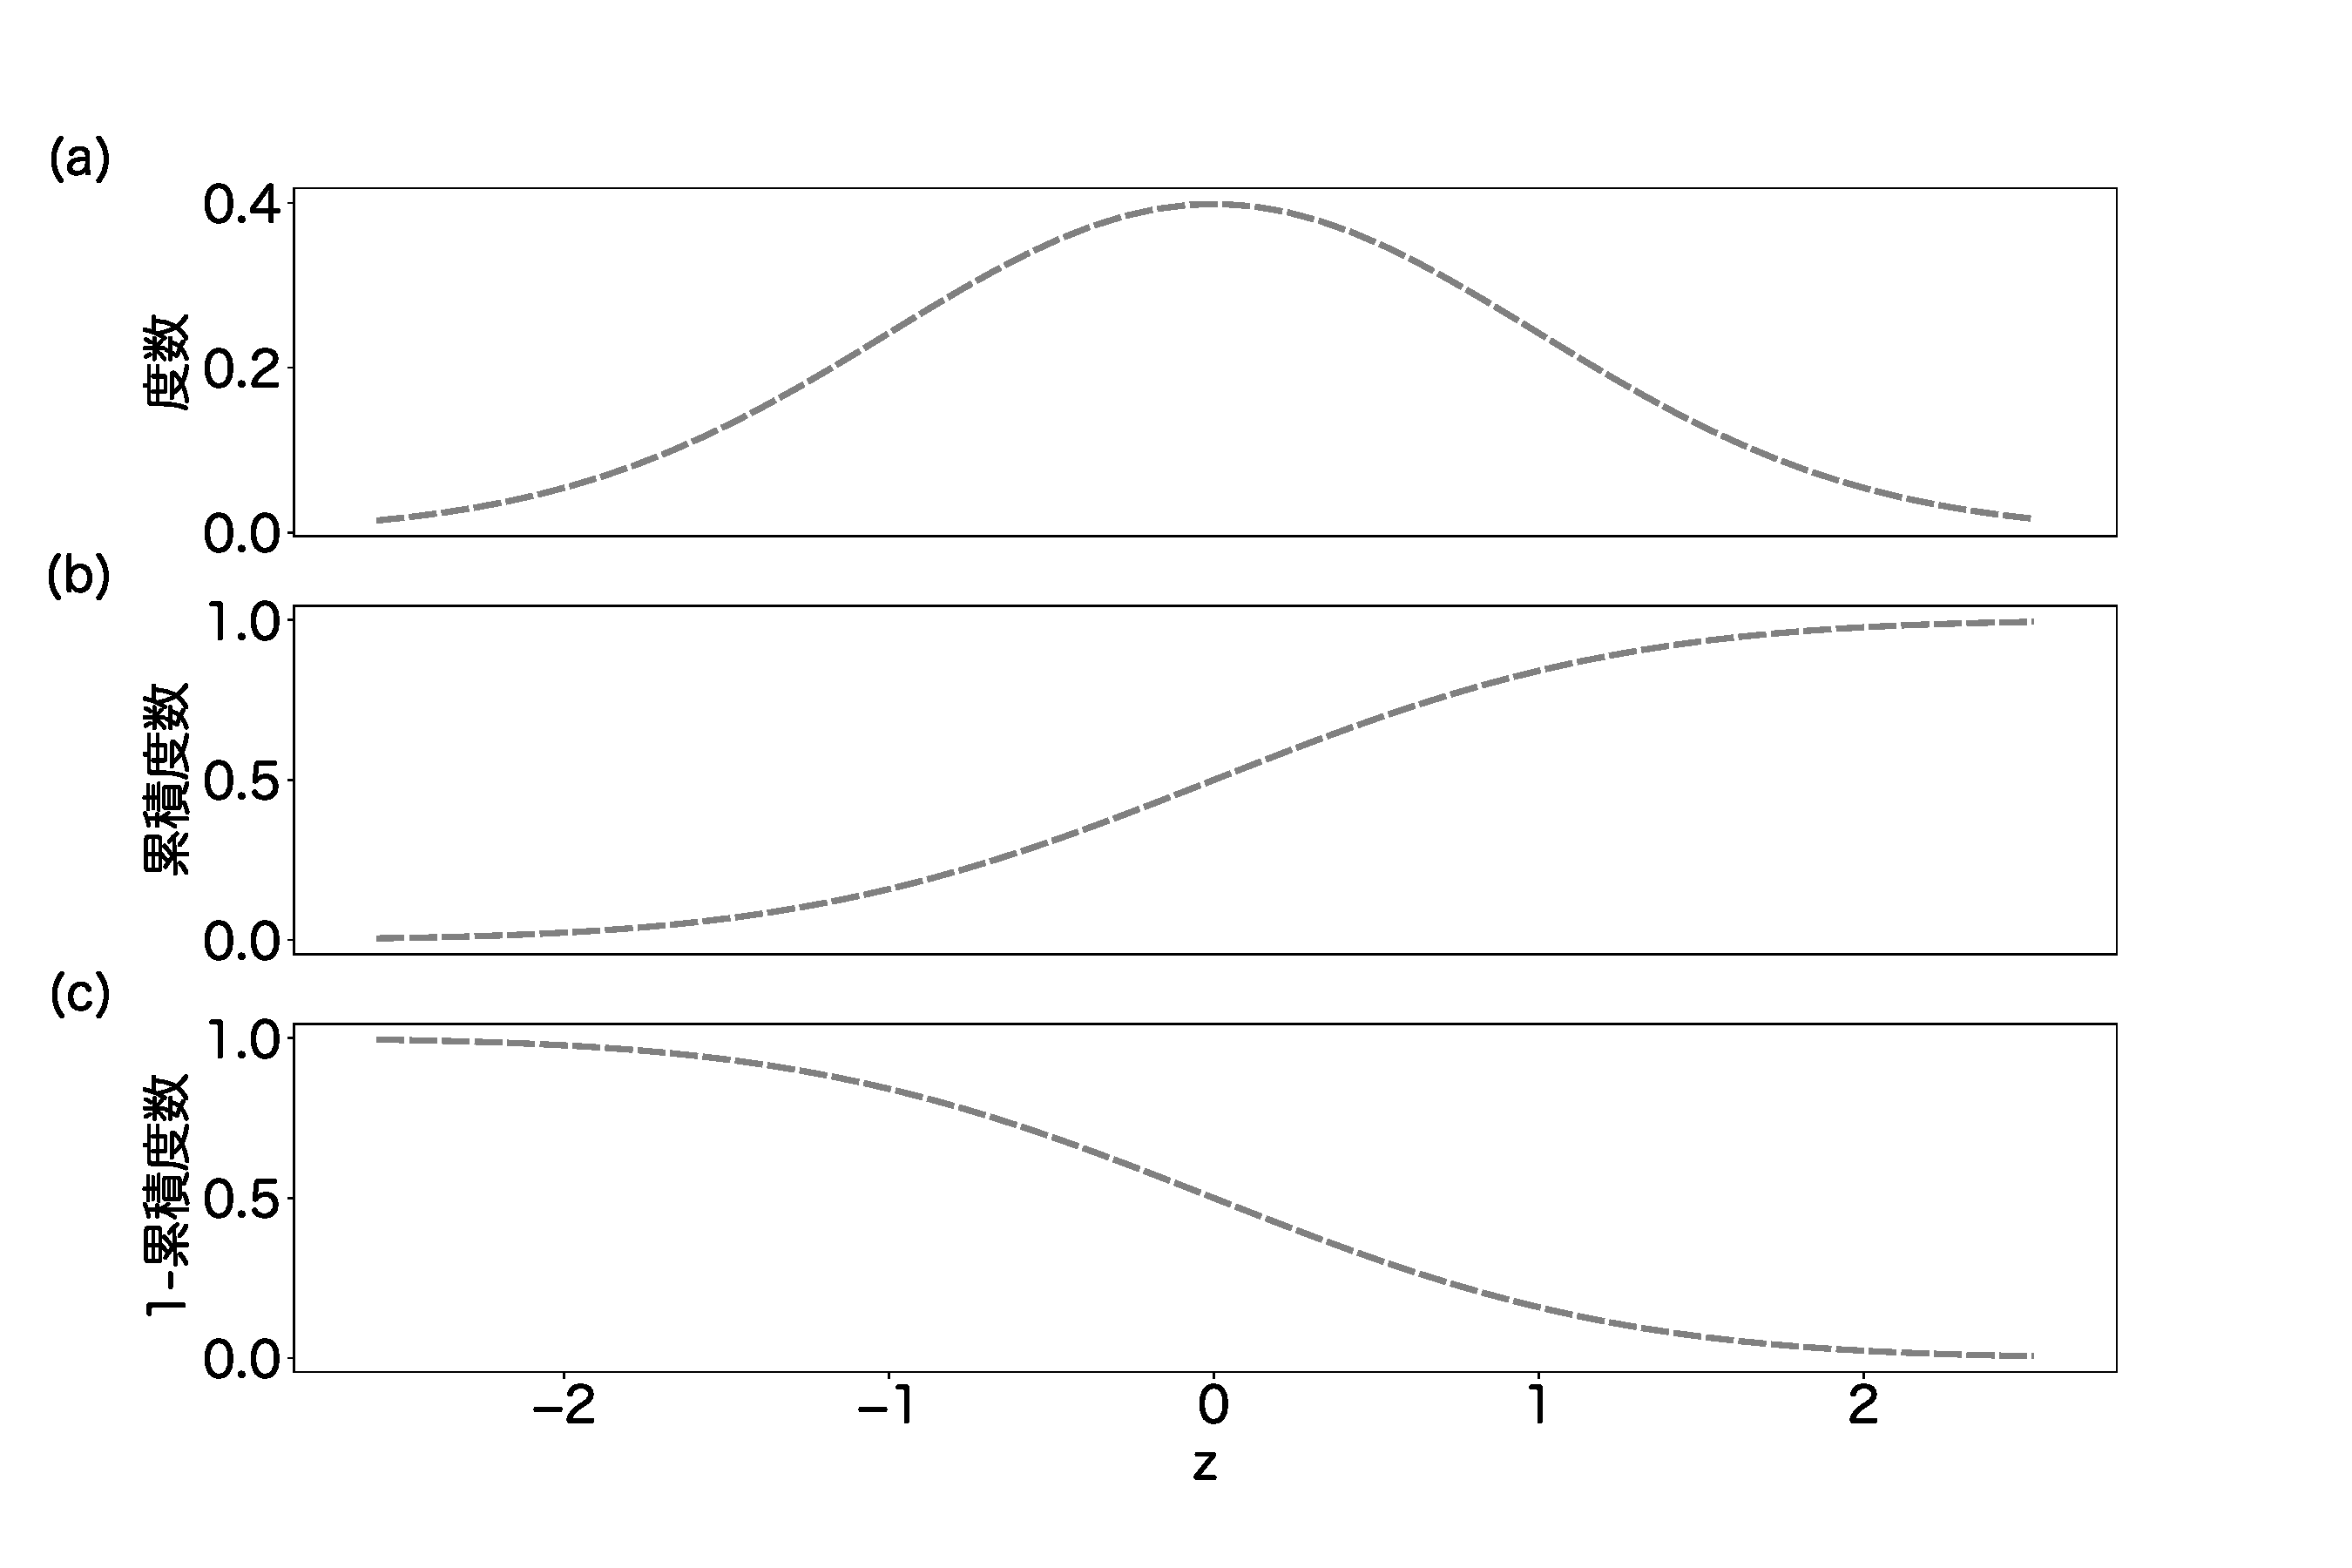
\includegraphics[width=15cm]{./image/02_/standard_normal.pdf}
        \caption{標準正規分布(a)確率密度関数(b)累積度数分布(c)1-累積度数分布}
        \label{fig:standard_normal_distribution}

    \end{center}
\end{figure}
    

\subsection{正規分布に従う確率変数の出現しやすさ1}
標準正規関数に従う確率変数が$95\%$の確率で見つかる範囲を求めてみます。
標準正規関数は、0を中心にして、対称な関数なので、正負の値が同じ程度の確率で見つかります。言い換えれば、$0\sim a$までの積分値と、$-a\sim 0$までの積分値が同じになります。そこで、次の積分を考えて、その最小値となる値を見つけてみます。
\begin{equation}
\int_{-a}^{a} \frac{1}{\sqrt{2\pi}}\exp(-\frac{z^2}{2}) dz = 0.95
\end{equation}

\begin{lstlisting}
b,a = norm.interval(0.95,0,1) # 積分値が0.95になる範囲を計算
print(norm.cdf(b, loc=0, scale=1)-norm.cdf(a, loc=0, scale=1)) # 0.95になるかを確認
print(b,a) # その範囲を表示
\end{lstlisting}


$0<\alpha<1$に対して、$\Phi(z_\alpha) = 1-\alpha$となる$z_\alpha$を上側$100\%$点という。
$z_{0.05}=1.64,z_{0.025}=1.96$の値は後でよく使う。

より、一般的には、$\alpha(0\leq \alpha \leq 0)$を指定すると、その半分$\alpha/2$となる積分範囲の末端を$a_1$とします。数式で書くと、
\begin{equation}
    \int_{-\infty}^{a_1} \frac{1}{\sqrt{2\pi}}\exp(-\frac{x^2}{2})dx = \frac{\alpha}{2}.
\end{equation}
同様に、右側の範囲の末端を$a_2$とします。数式で書くと、
\begin{equation*}
    \int_{a_2}^{\infty} \frac{1}{\sqrt{2\pi}}\exp(-\frac{x^2}{2})dx = \frac{\alpha}{2}.
\end{equation*}
これを書き換えると、次と同値です。
\begin{equation*}
    \int_{-\infty}^{a_2} \frac{1}{\sqrt{2\pi}}\exp(-\frac{x^2}{2})dx = 1-\frac{\alpha}{2}.
\end{equation*}

\begin{figure}
\begin{center}
    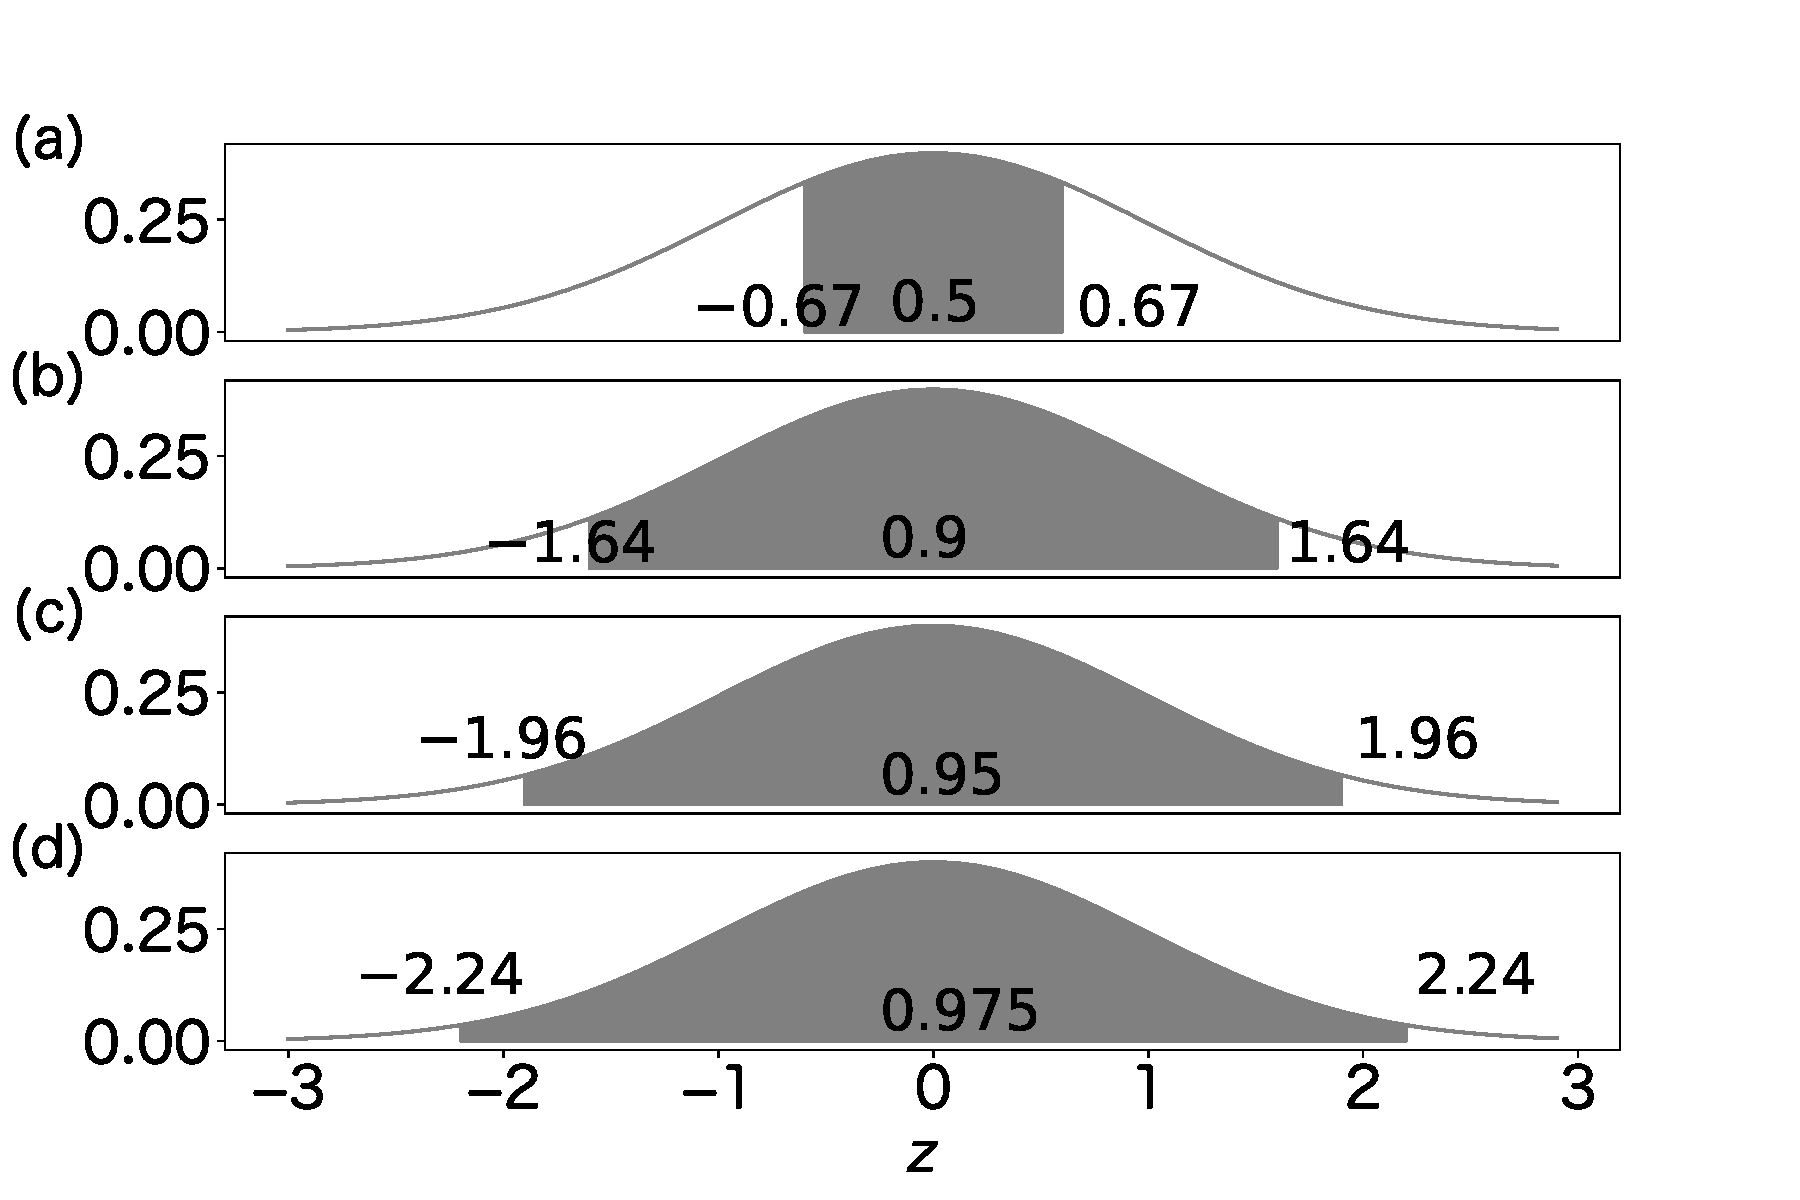
\includegraphics[width=15cm]{./image/02_/z_value.pdf}
    %\caption{図1.p値cm}
  \end{center}
\end{figure}

標準正規分布$z\sim N(0,1)$において$95\%$の確率で確率変数が見つかる範囲を調べることはできましたが、正規分布$x\sim N(\mu,\sigma^2)$においてでは、どの範囲になるのでしょう。次の定理を使えば簡単に計算ができます。
\begin{theo}
    確率変数$x$が、$x\sim N(\mu,\sigma^2)$であるならば、$\frac{x-\mu}{\sigma}\sim N(0,1)$である。    
\end{theo}
\begin{theo}
$\alpha(0\leq \alpha\leq 1)$に対して、$\int_{-\infty}^{z}\frac{1}{\sqrt{2\pi}}\exp(-x^2/2)=\alpha$を満たすとき、$\int_{-\infty}^{\mu+\sigma z} \frac{1}{\sqrt{2\sigma^2}}\exp(-\frac{(x-\mu)^2}{2\sigma})=\alpha$である。同様に、$\int_{z}^{-\infty}\frac{1}{\sqrt{2\pi}}\exp(-x^2/2)=1-\alpha$を満たす$z$について、$\int_{\mu+\sigma z}^{\infty} \frac{1}{\sqrt{2\sigma^2}}\exp(-\frac{(x-\mu)^2}{2\sigma})=1-\alpha$である。
\end{theo}
言い換えれば、標準正規分布の軸上の点$z$を、$[-\infty,z]$の範囲での積分値を保ったまま、正規分布$N(\mu,\sigma^2)$上の点に変換するには、$\frac{x-\mu}{\sigma}=z$を$x$について解けば良いことになります。

この定理により、以下をとけば、値が$95\%$の確率で得られる範囲がわかります。
\begin{eqnarray*}
    \frac{x-\mu}{\sigma}=z_{0.025}\\
    \rightarrow x = \mu+\sigma z_{0.025}
\end{eqnarray*}
また、
\begin{eqnarray*}
    \frac{x-\mu}{\sigma}=-z_{0.025}\\
    \rightarrow x = \mu-\sigma z_{0.025}
\end{eqnarray*}
以上により、$x \sim N(\mu,\sigma^2)$が$95\%$の確率で見つかる範囲は、$[\mu-\sigma z_{0.025},\mu+\sigma z_{0.025}]$であることがわかります。
同様に$90\%$の確率で見つかる範囲は、$[\mu-\sigma z_{0.05},\mu+\sigma z_{0.05}]$です。

\subsection{より大きな値をとる確率}
$x$を標準正規分布の確率変数とし、($x\sim N(0,1)$)また、$x\leq 0$であるとします。。$x$以上の大きな値を取る確率は、$P(X>x)=1-\varPhi(x)$で計算できます。
同様に、$x < 0$であるときは、より小さな値を取る値が、$P(x<X)=\varPhi(x)$で同様に計算できます。
図\ref{fig:z_value_larger}には、$x$に対して、より異なった値を取る確率を書いています。

$x$の大きさ$|x|$よりも大きな値を取る確率は、以上の二つの和で次のようにかけます。
\begin{equation}
    P(|x|>z) = 1-\varPhi(|x|)+\varPhi(-|x|)
\end{equation}
式を見ると正の数で$x$より大きな値を取る確率と、負の数で$x$より小さな値を取る確率の和になっていることが確認できます。
$P(|x|>z)$はより極端な値を取る確率などと言う方もされます。

計算してみます。$x=1.64$であれば、$\varPhi(1.64)=0.95$より、それ以上に大きな値を得る確率は、$P(X>1.64)=0.05$です。また、$x=-1.64$であれば、$\varPhi(-1.64)=0.05$です。よって、$|x|=|1.64|$よりも大きな値を得る確率は$P(|1.64|>X)=0.1$です。


\begin{figure}
    \begin{center}
        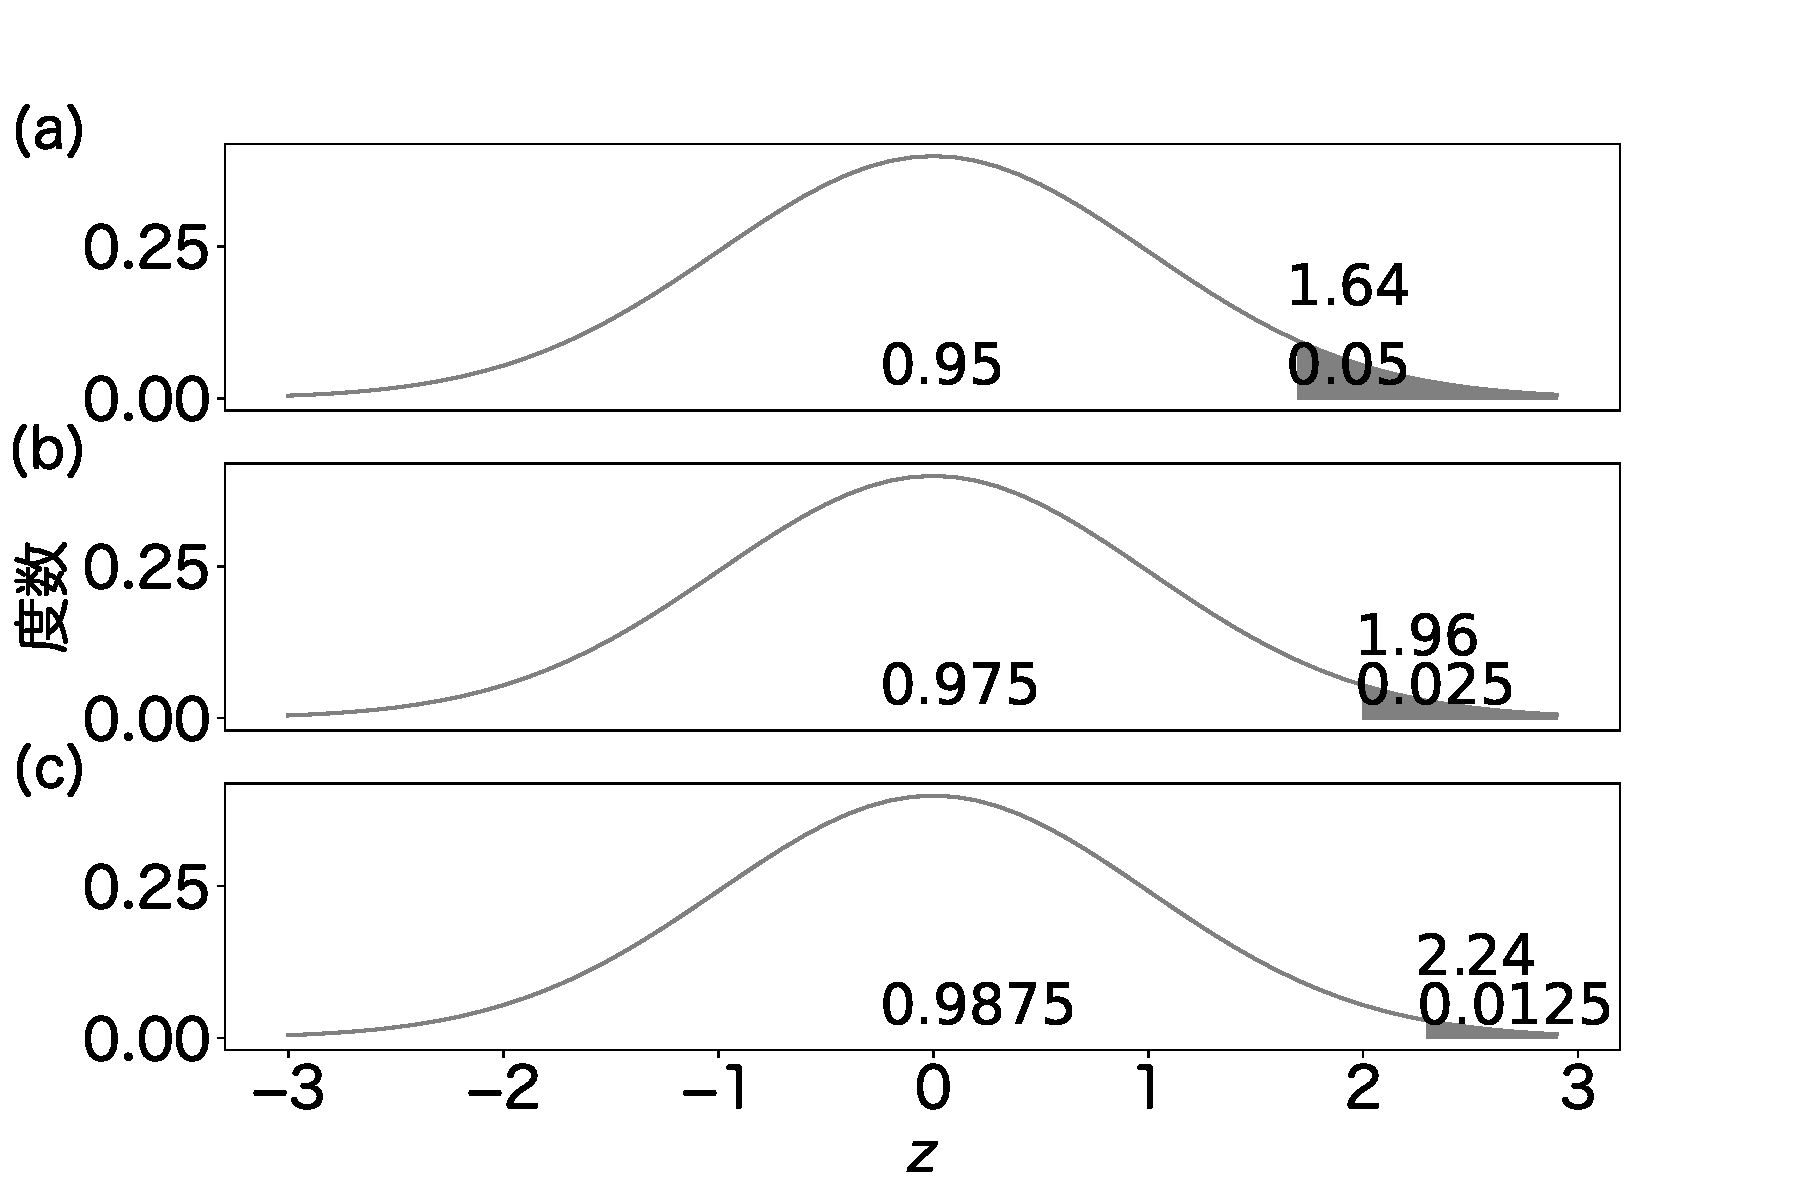
\includegraphics[width=15cm]{./image/02_/z_value_larger.pdf}
        \caption{標準正規分布におけるより大きな値(より偏った値)を取る確率。(a)$z=1.64$より大きな値を取る確率は0.05。(b)$z=1.96$より大きな値を取る確率は$0.025$。(c)$z=2.24$よりも大きな値を取る確率は$0.0125$}
        \label{fig:z_value_larger}
      \end{center}
    \end{figure}

\subsection{$N(0,1)$での珍しい値は、$N(0,2)$では珍しくない?}
以上の議論により、$N(0,1)$において、$z=1.64$以上の値が出る確率はおよそ$5\%$である。
では、$N(0,2)$において$z=1.64$が出る確率はいくつだろうか。
$N(0,2)$において、$z=1.64\times2$以上に大きな値が出る確率は、およそ$5\%$である。
このことから、$N(0,2)$において$z=1.64$以上の値が出る確率は、$5\%$より大きいことがわかる。
具体的に、計算をしてみると、その確率は$0.206$程度であることがわかる。
\begin{lstlisting}
1-norm.cdf(1.64,0,2)
\end{lstlisting}

\subsection{$N(1.96,1)$で出てくる値は、$N(0,1)$において珍しい?}
$N(1.96,1)$において、$1.96$以上の値が出る確率は、$50\%$です。明らかに、よく出る値であることがわかります。
一方で、$N(0,1)$においては、$1.96$以上の値が出る確率は、$2.5\%$くらいなので、珍しい値になります。
このように、確率分布の母数が変化すると、珍しい値も変化します。




\subsection{正規分布に従う確率変数の出現しやすさ2}
確率変数のしやすさを表す基準として、$\sigma$を基準にして、定数$a$倍の範囲$[\mu-a\sigma,\mu+a\sigma]$を使う方法もあります。
標準正規分布では、分散が$1$なので、その$0.5$倍、$1$倍、$2$倍、$3$倍の範囲はそれぞれ$[-0.5,0.5]$,$[-1,1]$,$[-2,2]$,$[-3,3]$になります。この範囲に入る確率は、それぞれ$0.38$,$0.683$,$0.954$,$0.997$です。それぞれの範囲と確率は、図\ref{fig:sigma_interval_probability}に図示しました。

$\sigma$の定数倍の範囲に値が見つかる確率は、$\sigma$の大きさに依存しないことが証明できます。言い換えれば、$[-0.5\sigma,0.5\sigma],[-\sigma,\sigma],[-2\sigma,2\sigma],[-3\sigma,3\sigma]$の範囲に値がある確率は、上記と同じで、それぞれおよそ$0.38$,$0.683$,$0.954$,$0.997$になります。


\begin{figure}
    \begin{center}
        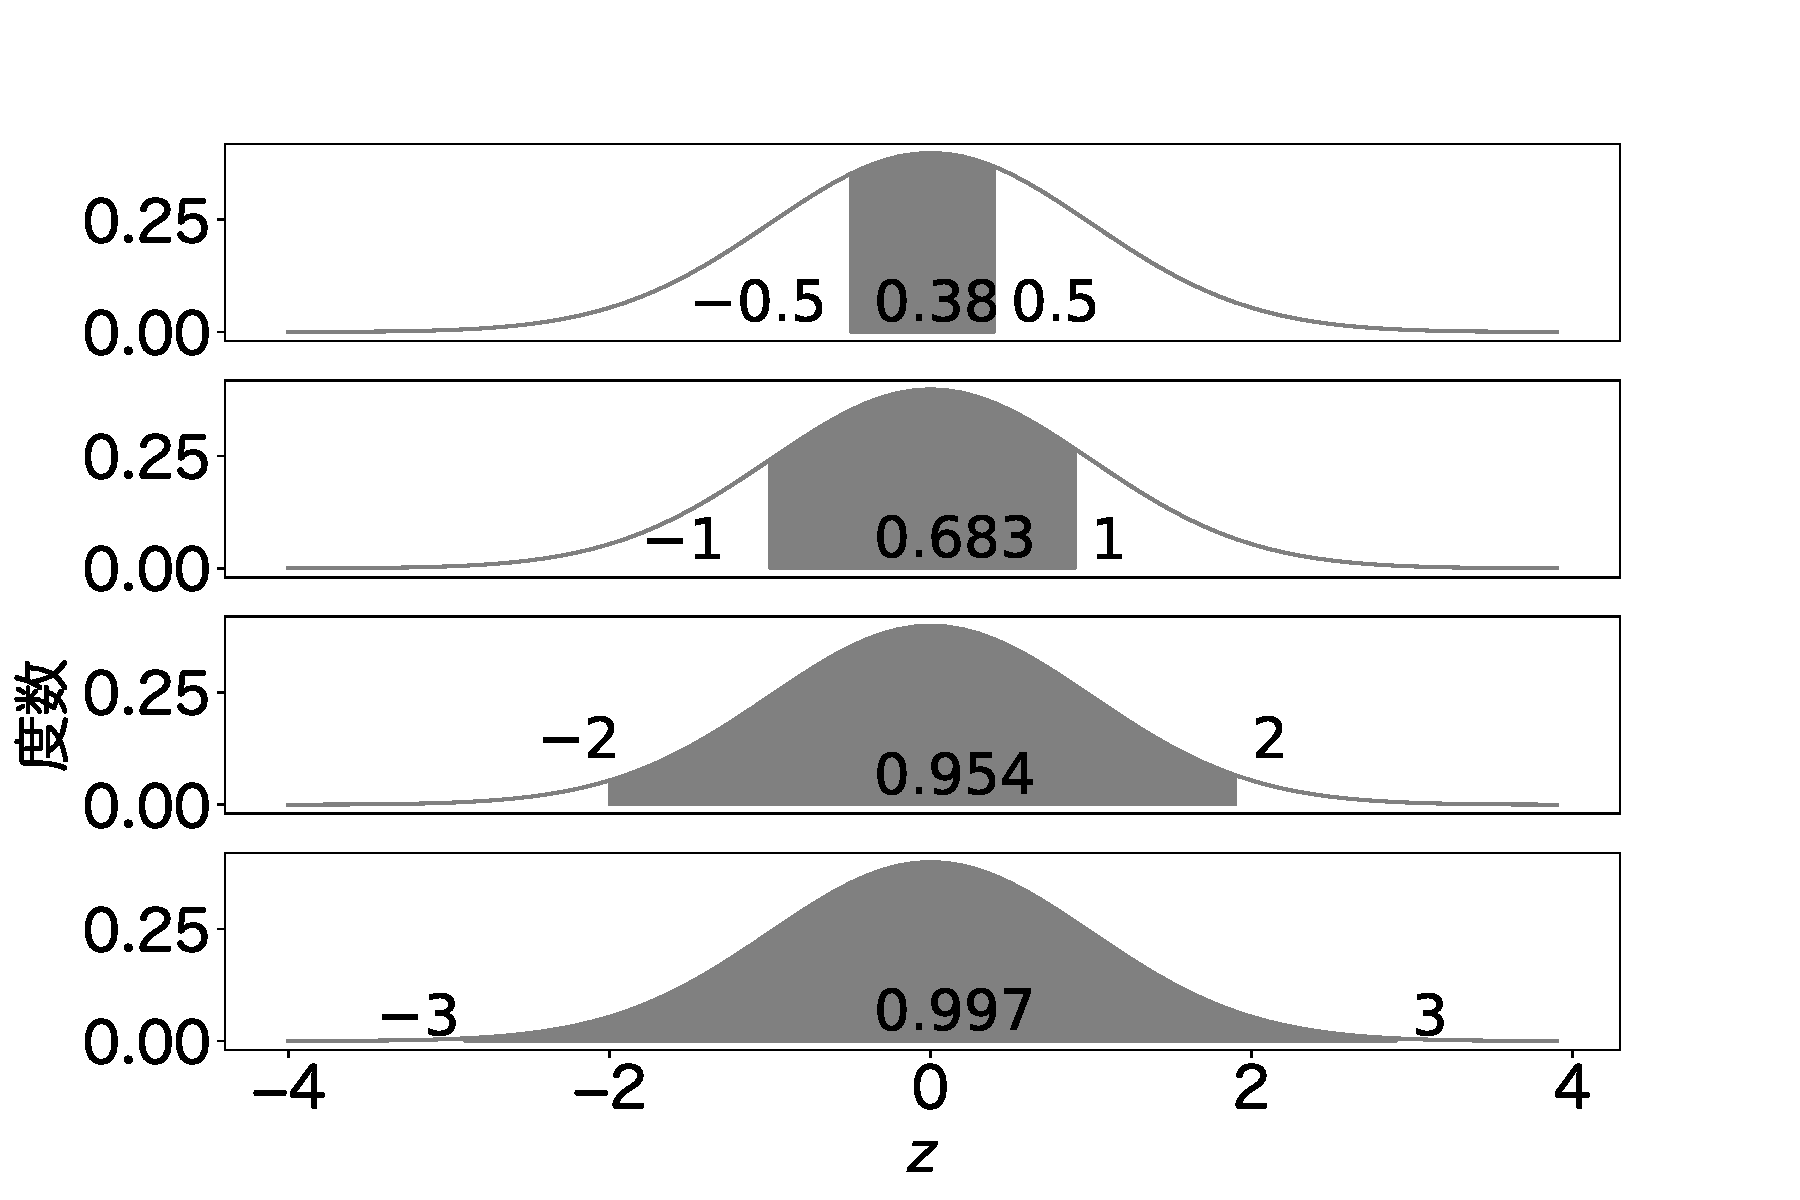
\includegraphics[width=15cm]{./image/02_/sigma_value.pdf}
        %\caption{図1.p値cm}
        \label{fig:sigma_interval_probability}
      \end{center}
\end{figure}

\begin{table}[hbtp]
    \caption{$\sigma$を基準にした値の出やすさ}
    %\label{table:data_type}
    \centering
    \begin{tabular}{lcr}
        \hline
        出現確率  & $N(0,1)$  &  $N(\mu,\sigma^2)$ \\
        \hline \hline
        0.38 & [-0.5,0.5]  & $[\mu-0.5\sigma,\mu+0.5\sigma]$ \\
        0.683 & [-1,1] & $[\mu-\sigma,\mu+\sigma]$\\
        0.954 & [-2,2] & $[\mu-2\sigma,\mu+2\sigma]$\\
        0.996 & [-3,3] & $[\mu-3\sigma,\mu+3\sigma]$\\
    \end{tabular}
\end{table}



\section{指数分布}
確率変数$X$が指数分布に従うことを$X \sim Exp(\lambda)$と書く。
指数分布の確率密度関数は、
\begin{equation*}
    f(x)=\lambda \exp(-\lambda x).
\end{equation*}
ここで、$\lambda$は、$\lambda>0$であり、指数分布の母数である。
期待値は$E[X]=\frac{1}{\lambda}$で、分散は、$V[X]=\frac{1}{\lambda^2}$である。
累積分布関数は、
\begin{equation*}
    F(x)=1-\exp(-\lambda x).
\end{equation*}
正規分布は、母数平均を中心として、左右対称に分布していた。言い換えれば、$\phi(\mu+x)=\phi(\mu-x)$である。一方で、指数分布は、左右非対称に分布が広がり、小さな値は大きな値よりも出現確率が高いので、$f(E[X]+a)\neq f(E[X]-a)$である。
また、正規分布では、母数平均と母数分散がそれぞれ独立なので、それぞれの特徴を独立に動かすことで、期待値や分散が独立に変化する。
指数分布では、母数が一つであり、母数を変化させると、期待値と分散は同時に変化する。



\begin{figure}
    \begin{center}
        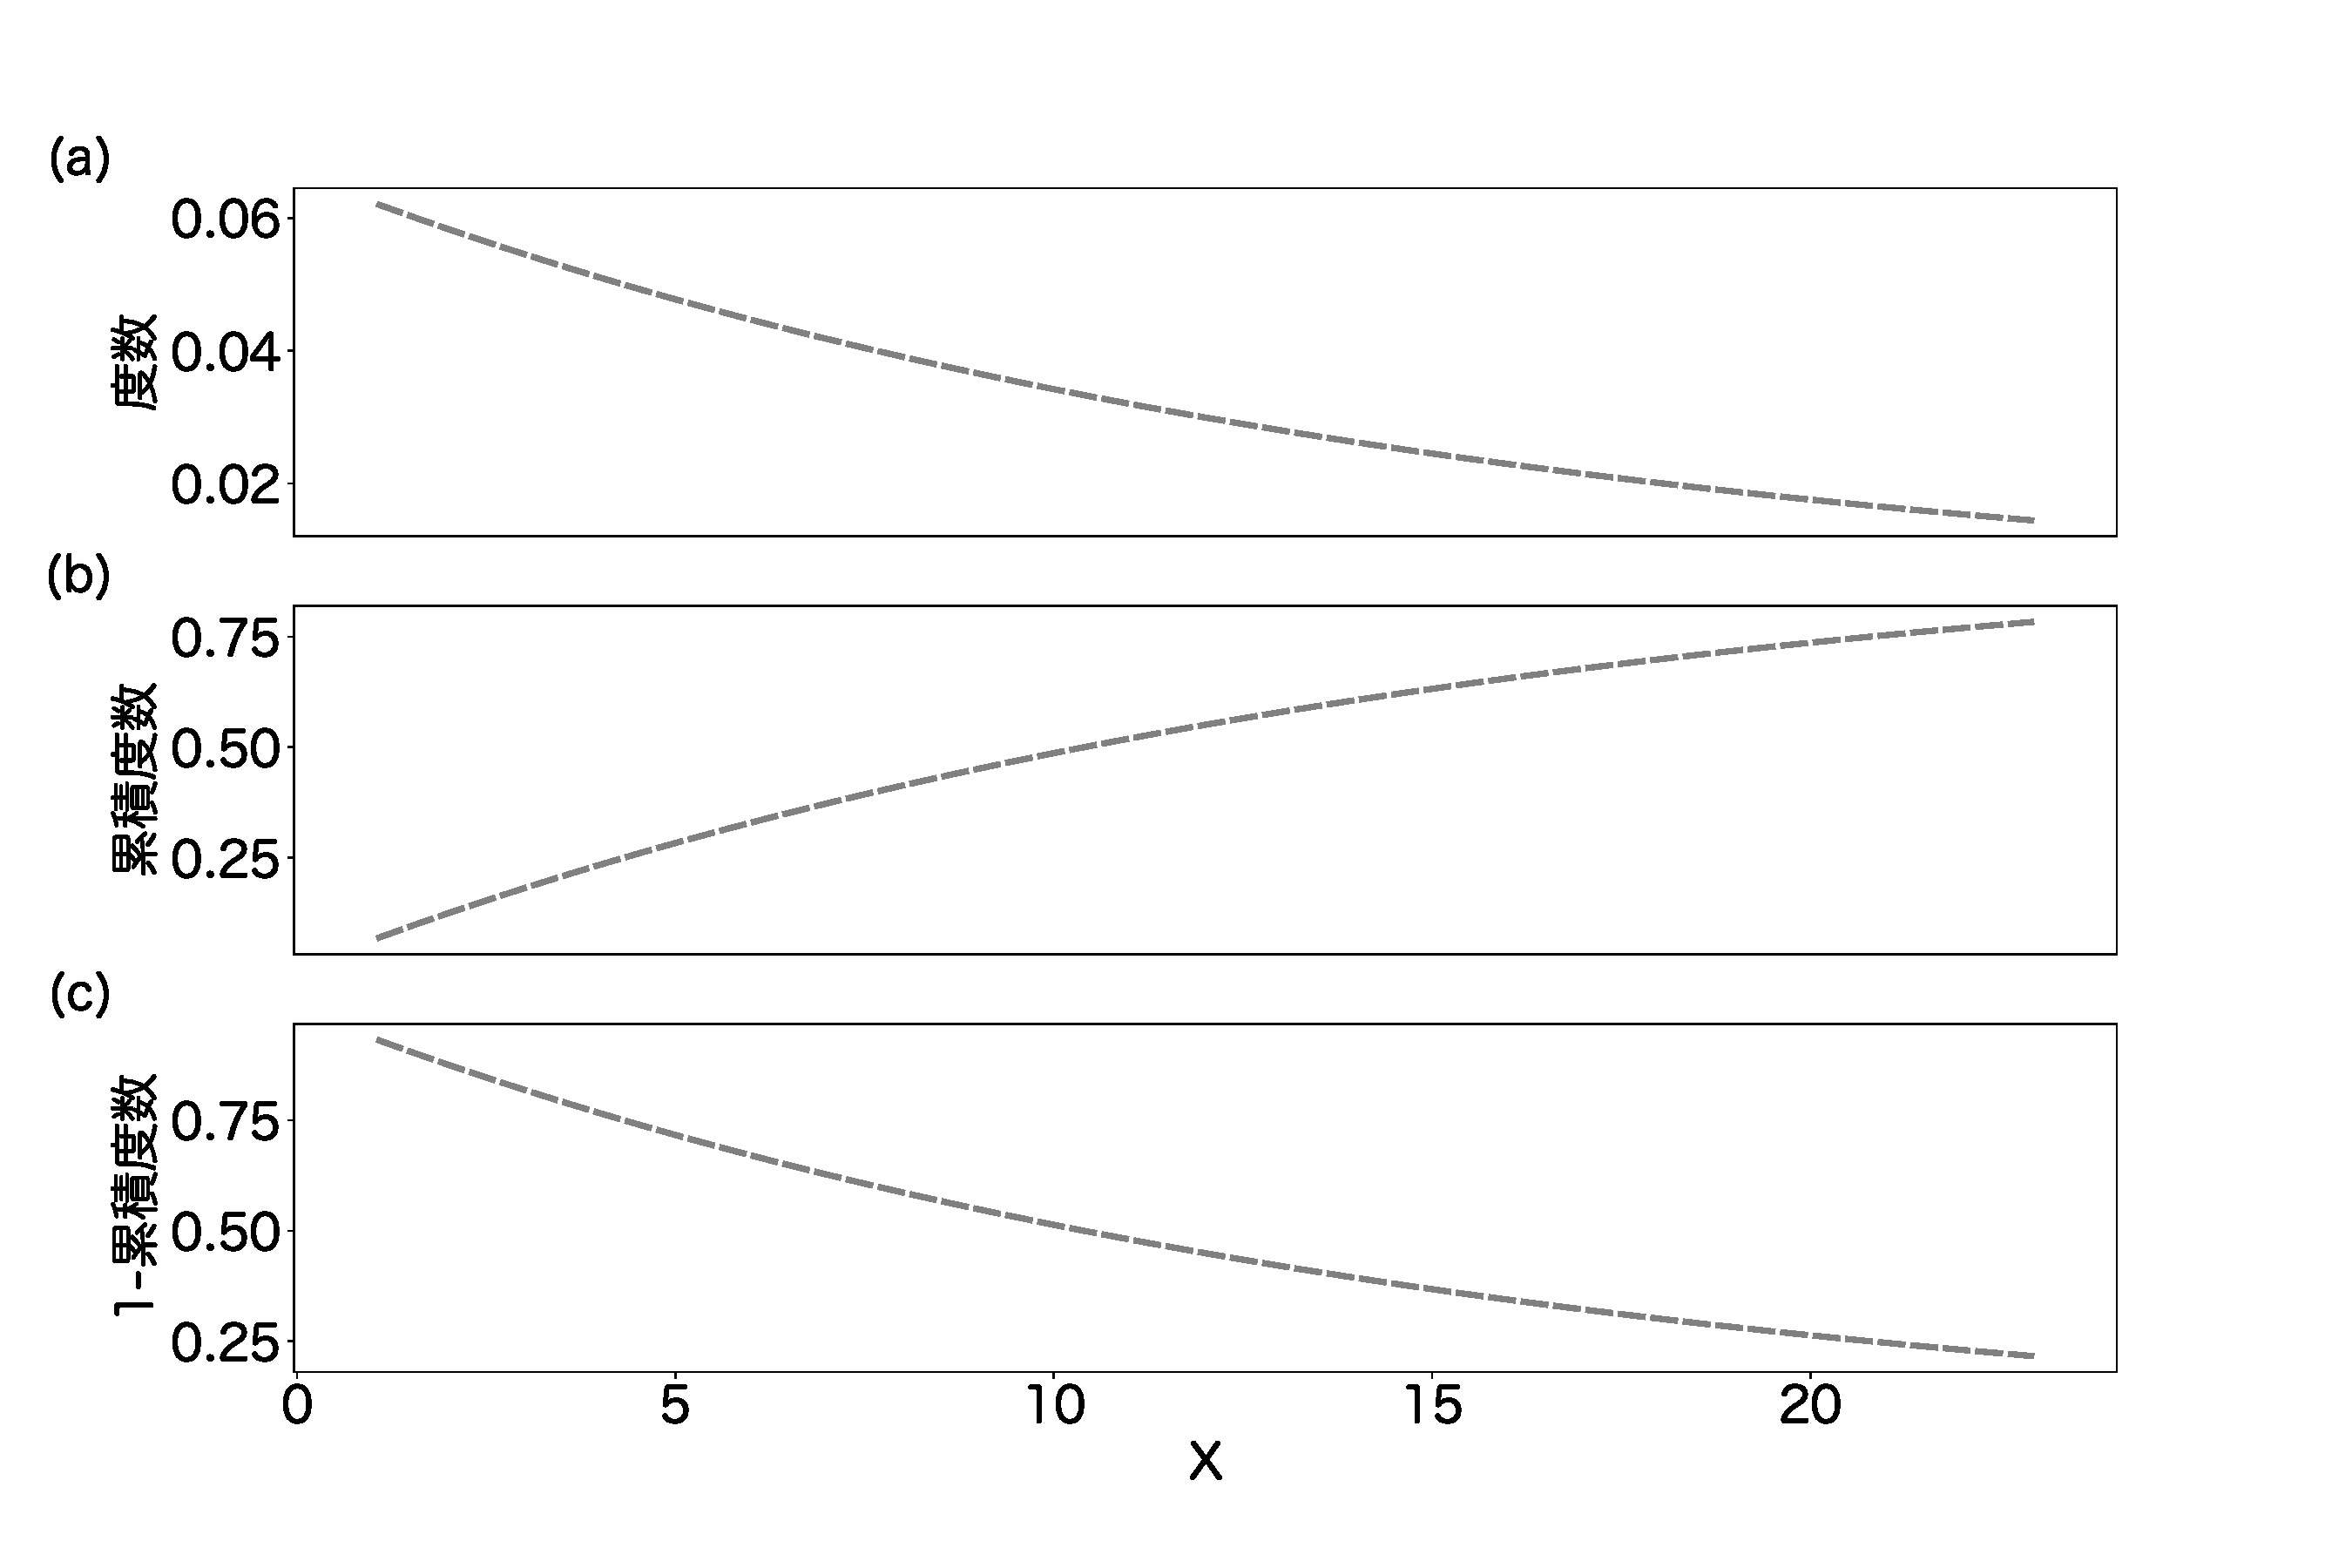
\includegraphics[width=15cm]{./image/02_/expon_frequency.pdf}
        \caption{指数分布$\lambda=1/15$(a)確率密度関数(b)累積度数分布(c)相補累積度数分布}
        \label{expon_frequency}
    \end{center}
\end{figure}


\subsection{指数分布に従う確率変数の出現しやすさ}
指数分布の確率密度関数を区間$[a,b]$で積分したときに、$\alpha(0\leq \alpha \leq 1)$になる$[a,b]$を求めます。条件として、
\begin{eqnarray*}
    \int_0^{a}  \lambda\exp(-\lambda x )dx &=& \alpha/2\\
    \int_0^{b} \lambda\exp(-\lambda x )dx &=& 1-\alpha/2
\end{eqnarray*}
を満たすとする。
$a$について、とくと、
\begin{eqnarray*}
    \int_0^{a}  \lambda\exp(-\lambda x )dx &=& \alpha/2\\
     1-\exp(-\lambda a) &=& \frac{\alpha}{2}\\
     \rightarrow a&=& \frac{1}{\lambda} \log\frac{1}{1-\alpha/2}
\end{eqnarray*}
$b$については、同様に、
\begin{equation*}
    b = \frac{1}{\lambda}\log\frac{\alpha}{2}
\end{equation*}
以上より、この積分の条件で、$100(1-\alpha)\%$の確率で値を得る範囲は、$[\frac{1}{\lambda} \log\frac{1}{1-\alpha/2} ,\frac{1}{\lambda}\log\frac{\alpha}{2}]$である。
図\ref{fig:expon_simulation_sample}は、指数分布により、サンプルサイズ$1000$の標本を$100$回作って、各標本においてデータが区間$[\frac{1}{\lambda} \log\frac{1}{1-\alpha/2} ,\frac{1}{\lambda}\log\frac{\alpha}{2}]$に入った割合をシミュレーションし、そのヒストグラムを表示している。確かに、$95\%$くらいの割合でその区間にデータが入っている。


\begin{figure}
    \begin{center}
        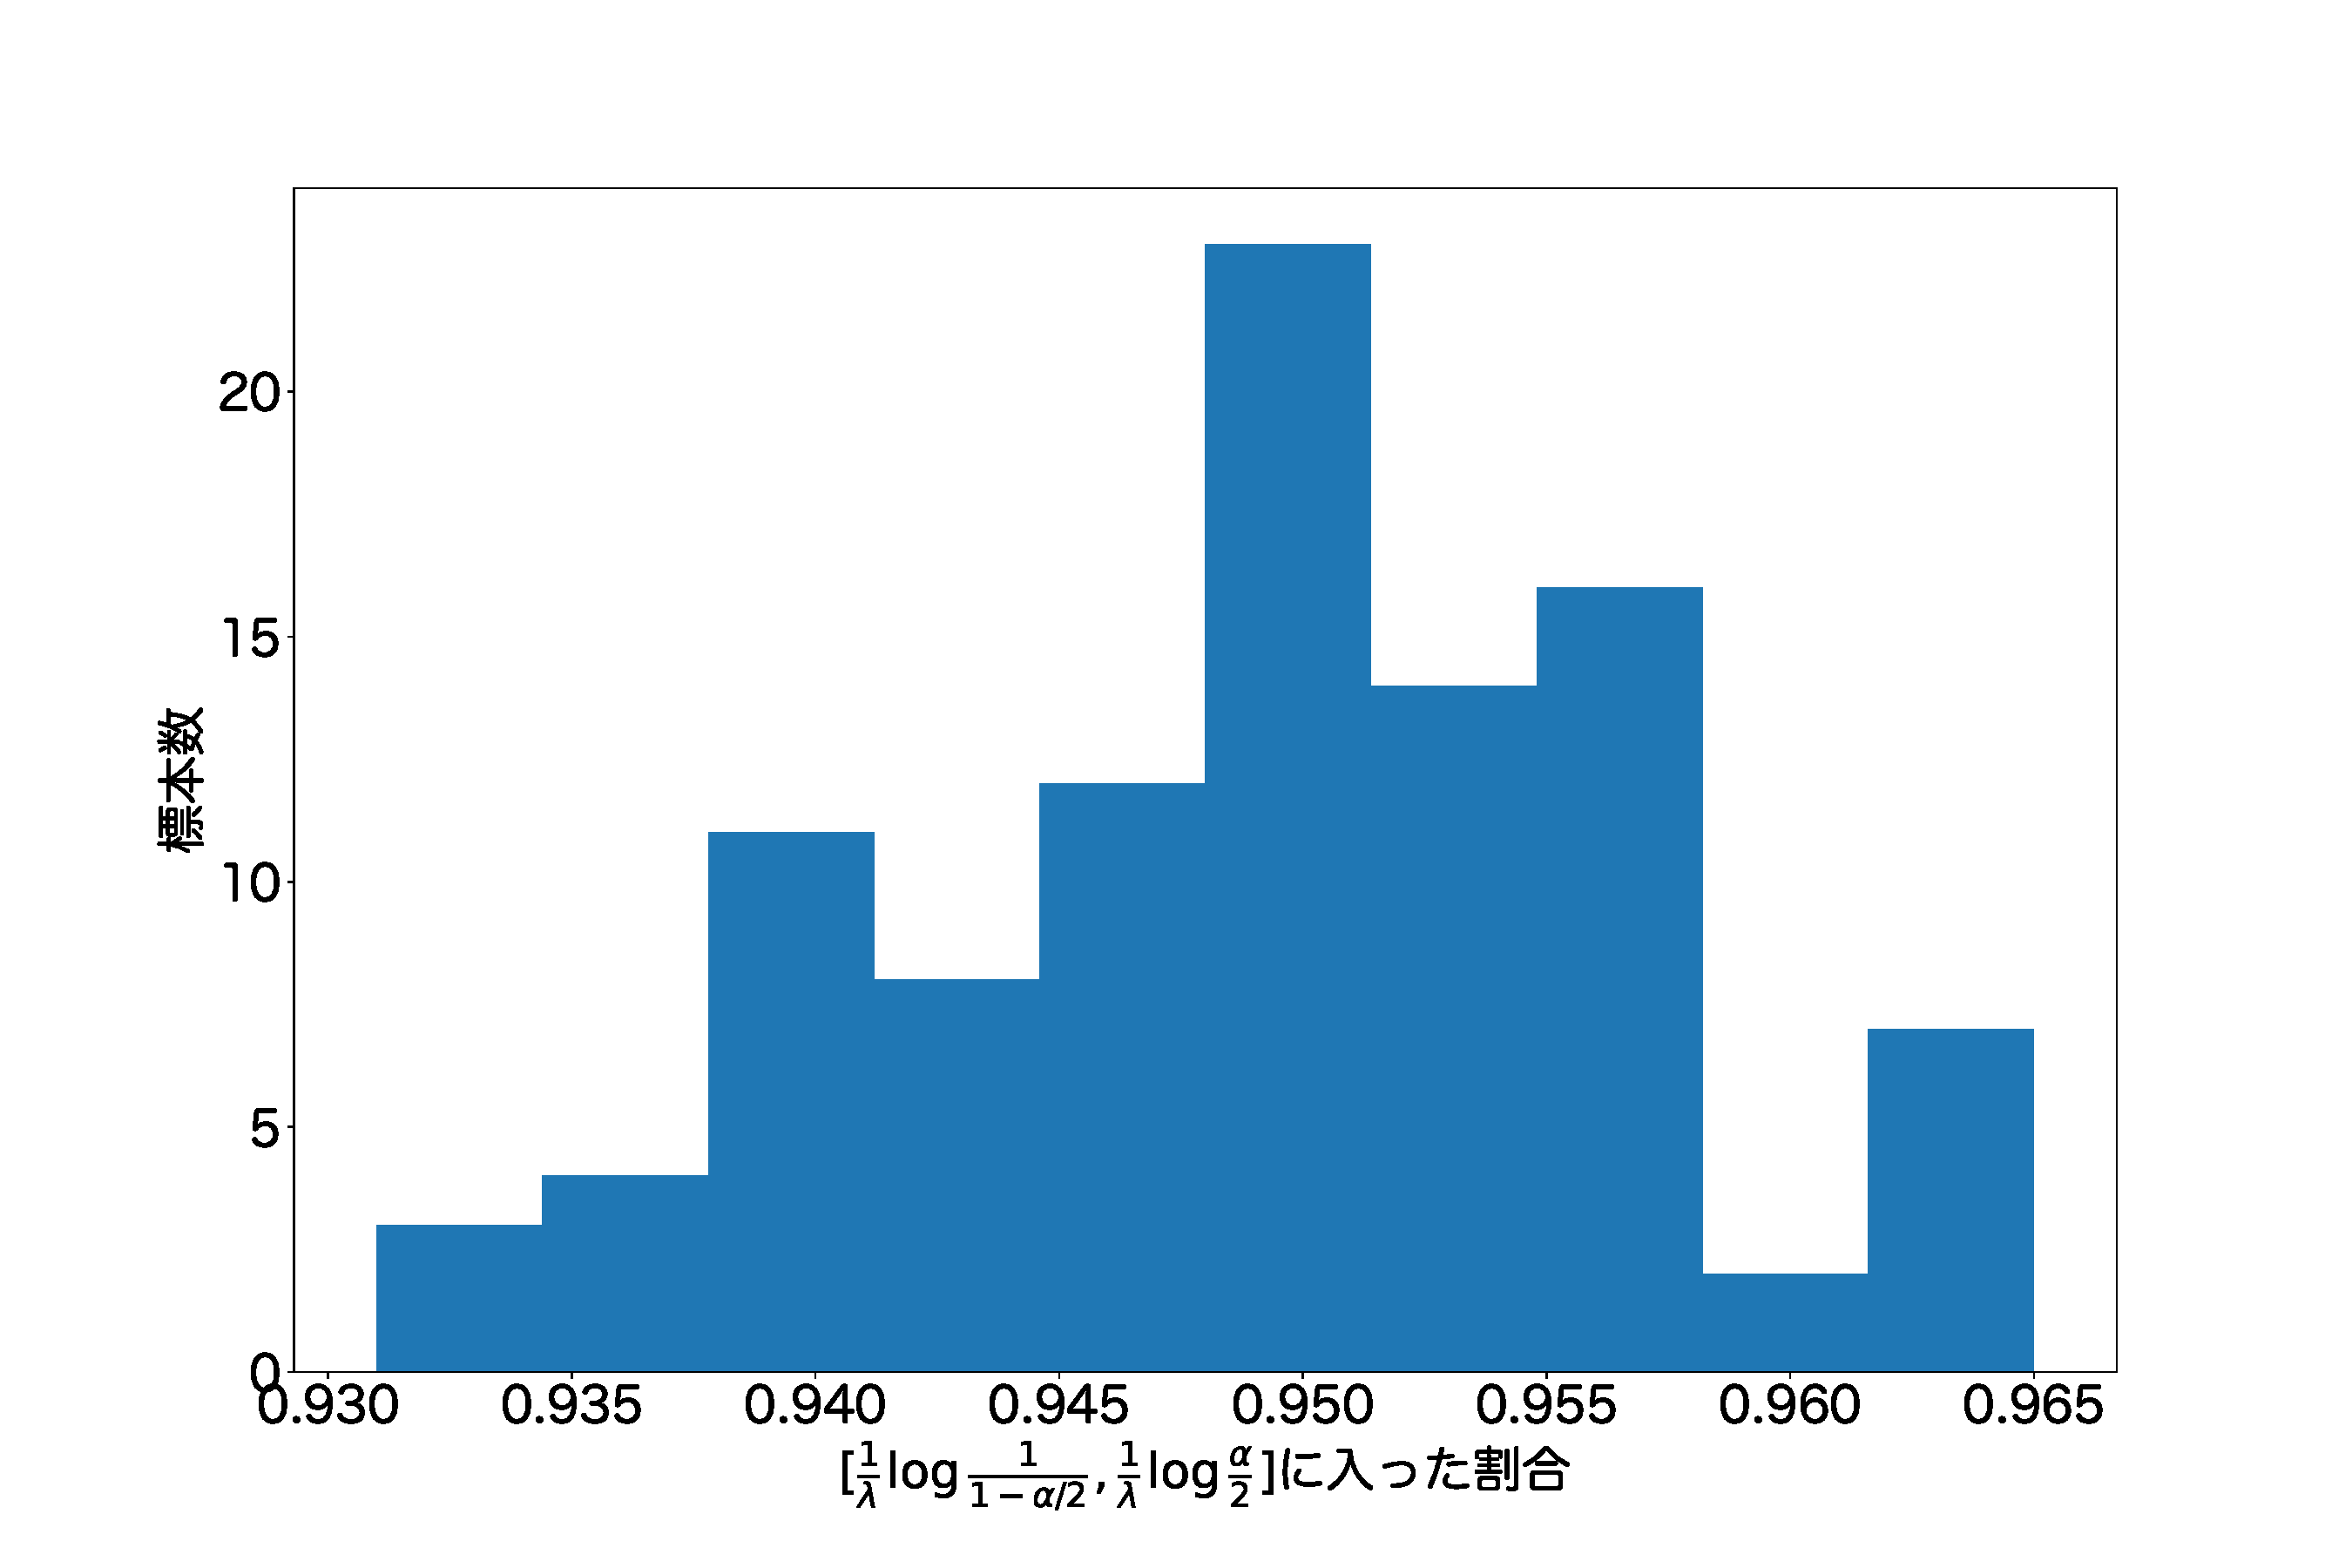
\includegraphics[width=15cm]{./image/02_/expon_simulation_sample.pdf}
        \caption{指数分布$\lambda=1/10$からサンプルサイズ1000の標本を100回シミュレーションし、各標本においてデータが区間$[\frac{1}{\lambda} \log\frac{1}{1-\alpha/2} ,\frac{1}{\lambda}\log\frac{\alpha}{2}]$に入った割合を計算した。そのヒストグラム。}
        \label{fig:expon_simulation_sample}

    \end{center}
\end{figure}


\section{カイ二乗分布}
確率変数$X$がカイ二乗分布に従うことを$X \sim \chi^2_k$と書く。ここで、$k$はカイ二乗分布の母数で、自由度を示し、自然数を取る。
確率密度関数は、
\begin{equation*}
    f(x;k) = \frac{1}{2^{k/2}\Gamma(k/2)}x^{k/2-1}\exp\left(-\frac{x}{2}\right).
\end{equation*}
ここで、$\Gamma(k/2)$はガンマ関数を表す\footnote{$ \Gamma(z)=\int_0^{\infty }t^{z-1}\exp(-t)dt$である。 }。
累積分布間数は、
\begin{equation*}
    F(x) = \frac{\gamma(k/2,x/2)}{\Gamma(k/2)}.
\end{equation*}
ここで、$\gamma(k/2,x/2)$は、不完全ガンマ関数である\footnote{$\gamma(a,x)=\int_0^x t^{a-1}\exp^{-t}dt$である。ガンマ関数も、不完全ガンマ関数も計算できなくても問題はない。コンピュータを使えばすぐに計算してくれる。}。
この関数も左右非対称である。


\begin{figure}
    \begin{center}
        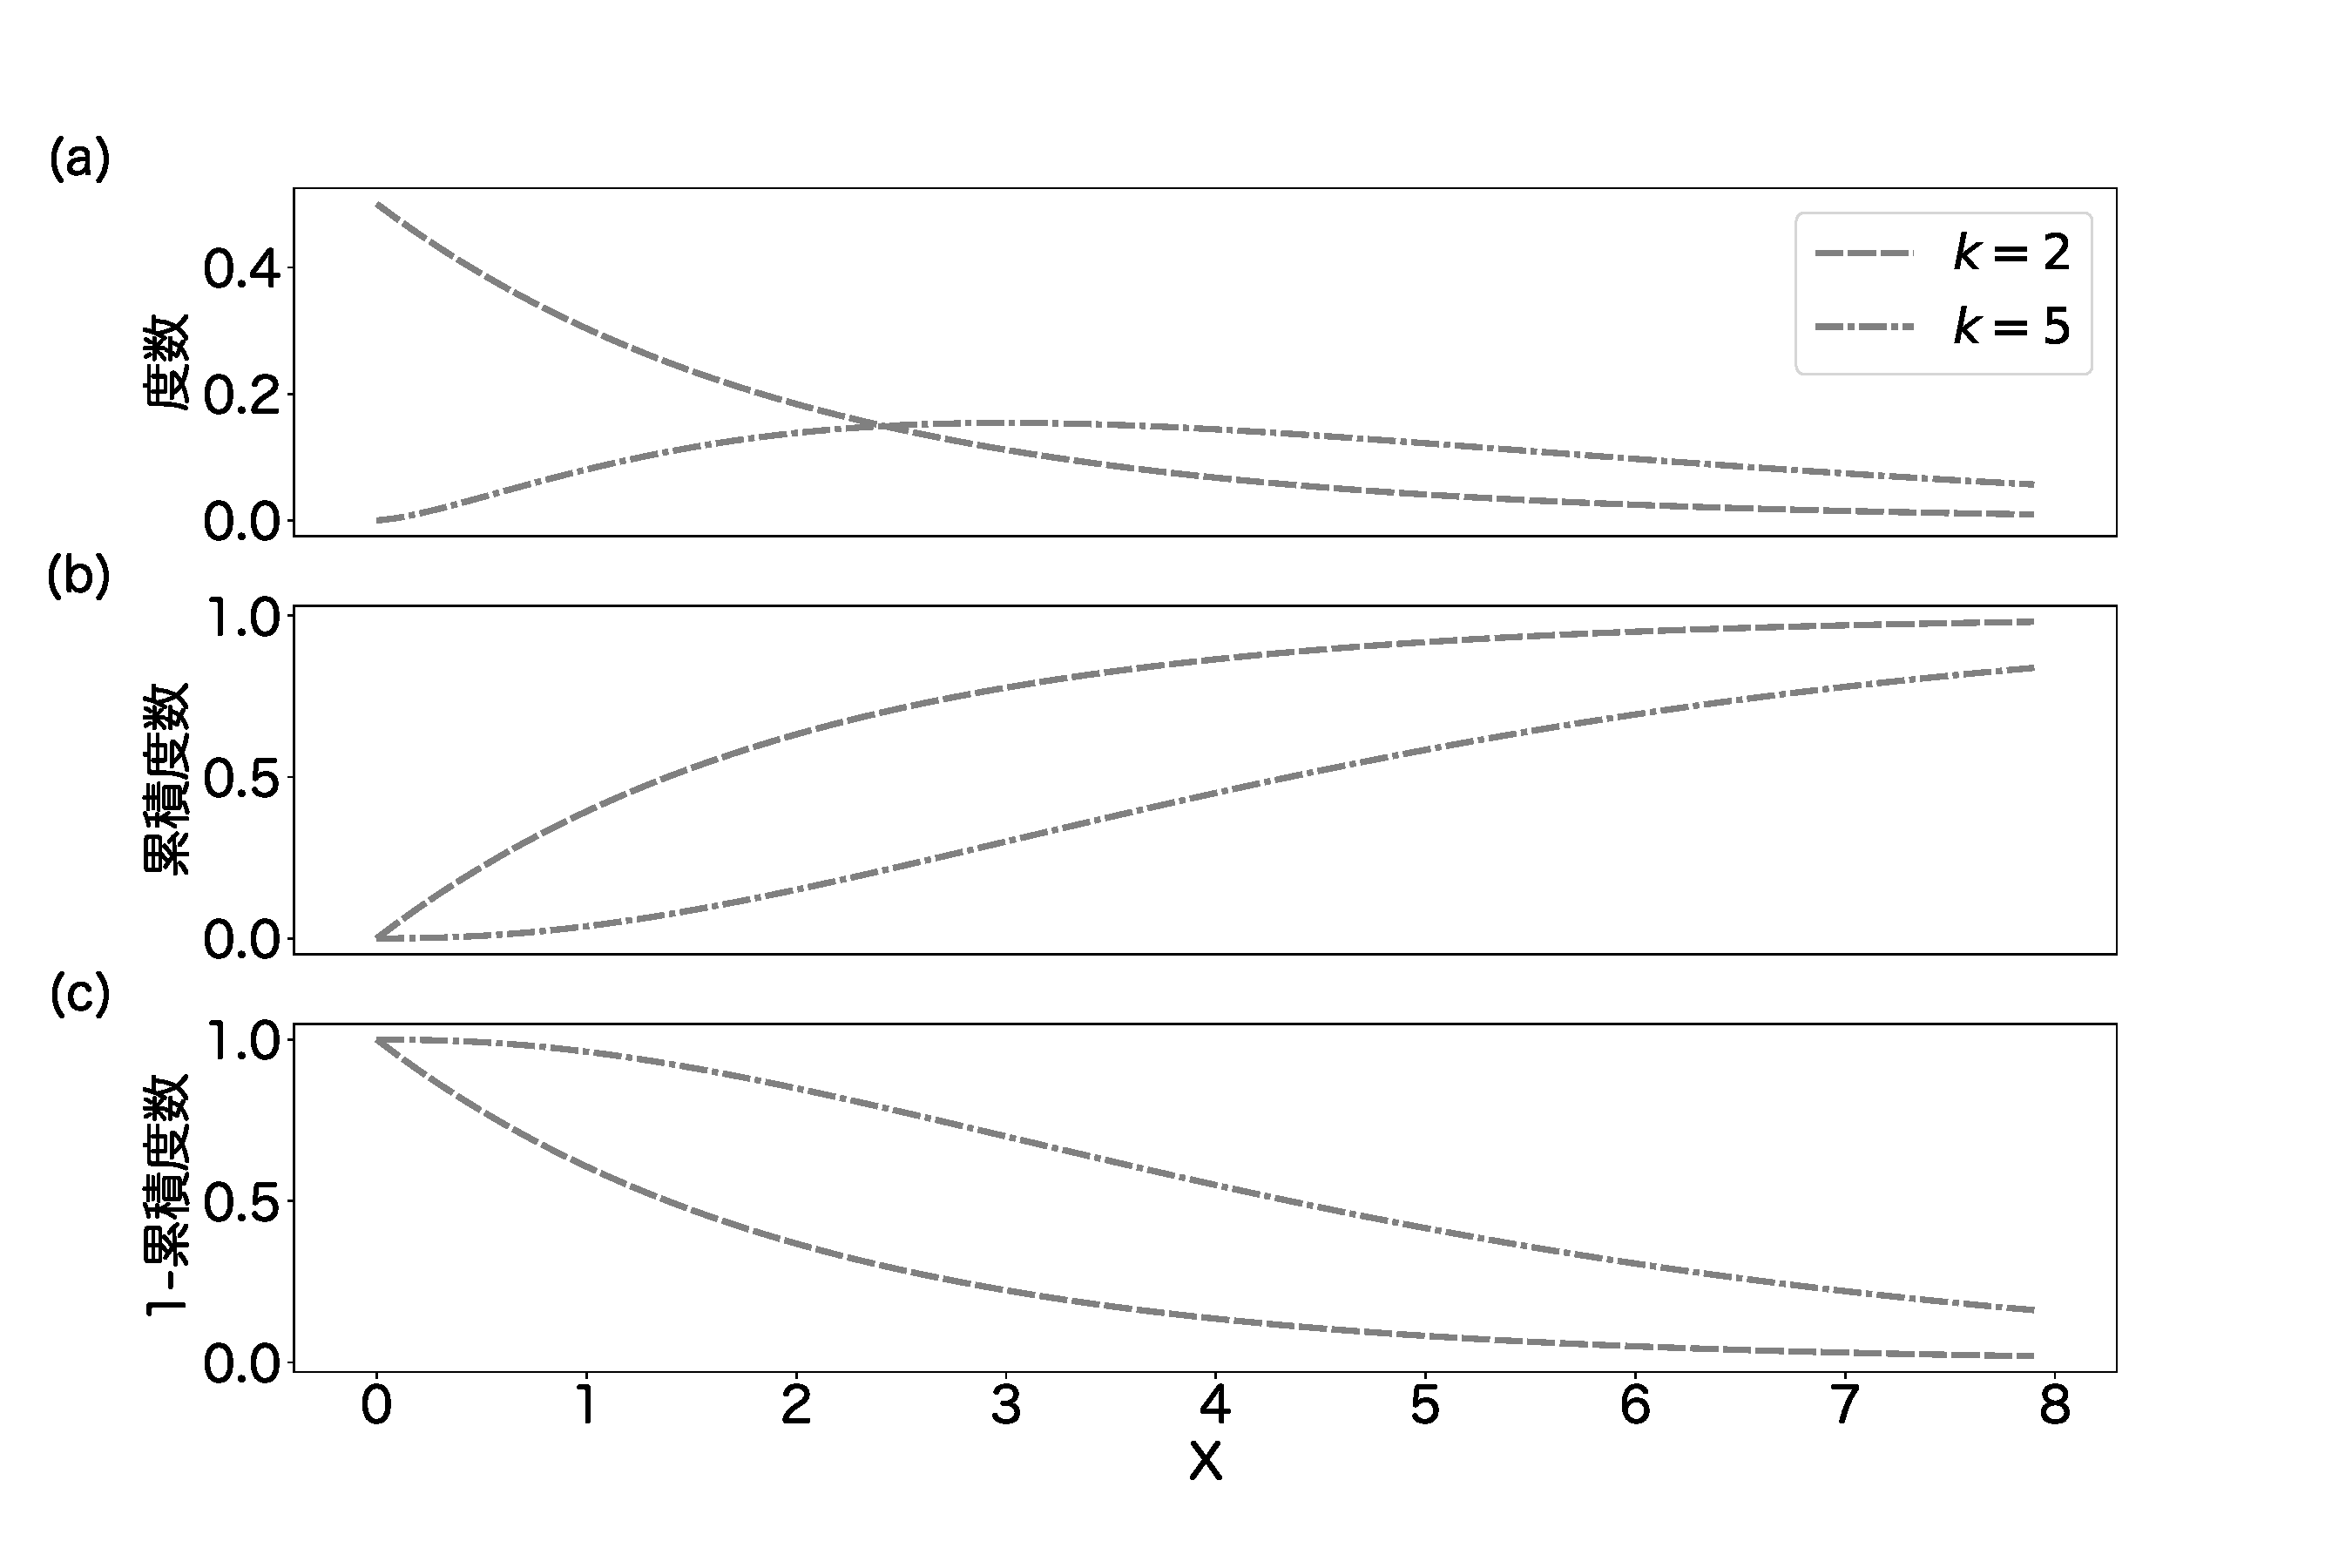
\includegraphics[width=15cm]{./image/02_/chi2_frequency.pdf}
        \caption{カイ二乗分布}
        \label{chi2_}
    \end{center}
\end{figure}

\subsection{カイ二乗分布に従う確率変数の出現しやすさ}
カイ二乗分布の確率密度関数を区間$[a,b]$で積分したときに、$\alpha(0\leq \alpha \leq 1)$になる$[a,b]$を求めます。条件として、
\begin{eqnarray*}
    \int_0^{a}  \frac{1}{2^{k/2}\Gamma(k/2)}x^{k/2-1}\exp\left(-\frac{x}{2}\right)dx &=& F(a)-F(0) = \alpha/2\\
    \int_0^{b} \frac{1}{2^{k/2}\Gamma(k/2)}x^{k/2-1}\exp\left(-\frac{x}{2}\right)dx &=& F(b)-F(0)= 1-\alpha/2
\end{eqnarray*}
を満たすとする。
代数的に$a,b$について解くことが難しいので、数値的に計算してみた結果を載せておく(表\ref{table:chi2_confidence})。この$a,b$をそれぞれ$\chi^2_k(\alpha),\chi^2_{k}(1-\alpha)$と書くことがある。


\begin{table}[hbtp]
    \caption{$\alpha=0.05$}
    \label{table:chi2_confidence}
    \centering
    \begin{tabular}{lcc}
    %\hline
    k  & $a$   & $b$   \\
    \hline \hline
    1 &  0.0009 &  5.02\\
    3 & 0.215 & 9.3484  \\
    5 &  0.831 & 12.832 \\
      \hline
    \end{tabular}
  \end{table}

\section{$t$分布}
確率変数$T$が$t$分布に従うとき、$T \sim t(\nu)$と表記する。
確率密度関数は、
\begin{equation*}
    f(t) = \frac{\Gamma((\nu+1)/2)}{\sqrt{\nu \pi}\Gamma(\nu/2) }(1+t^2/\nu)^{-(\nu+1)/2}.
\end{equation*}
ここで、$\nu$は、$0$より大きな実数である。
この関数を見ただけでは、すぐには判別するのは難しいかもしれないが、$f(t)$には$t$が関係する部分は$(1+t^2/\nu)$だけである。二乗の項があるので、偶数関数であることがわかり、$0$を中心にした対称な関数$f(t)=f(-t)$であることがわかる。
累積分布関数は著者には難しすぎるので、記述しない。wikipediaなどで調べれば正しそうな数式が書かれている。



\begin{figure}
    \begin{center}
        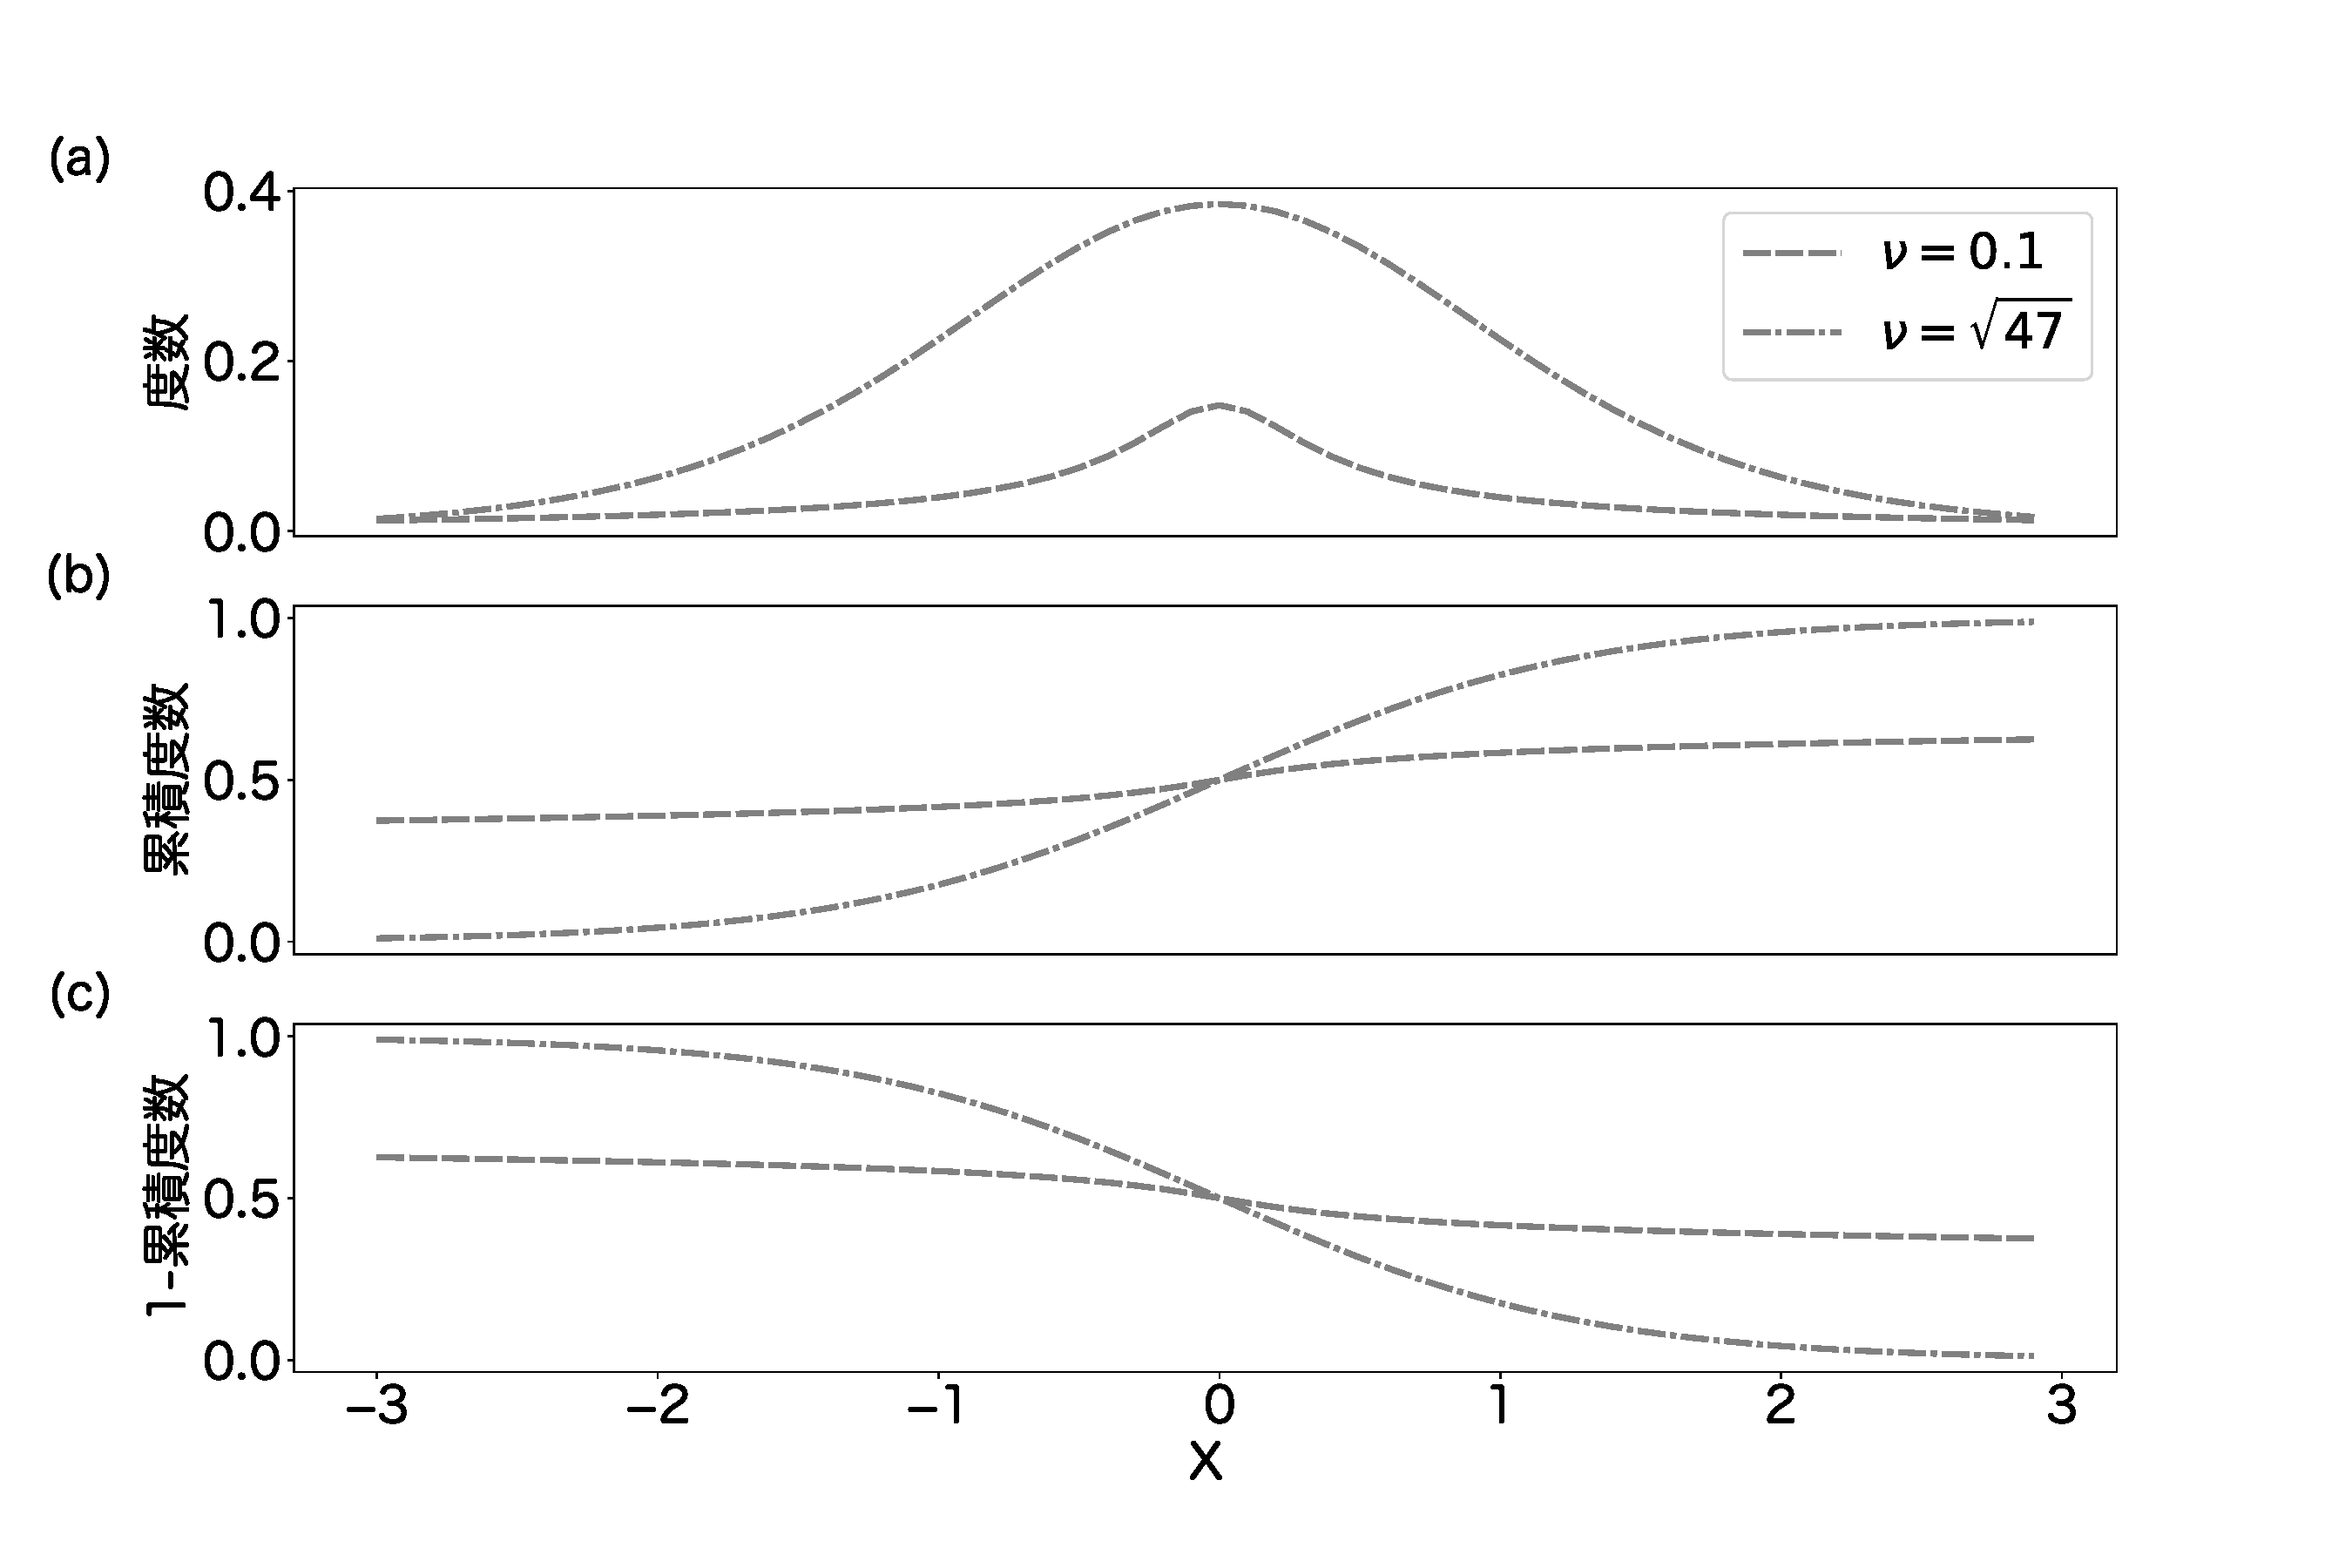
\includegraphics[width=15cm]{./image/02_/student_t_frequency.pdf}
        \caption{t分布}
        \label{student_t}
    \end{center}
\end{figure}

\subsection{$t$分布における珍しい値}
$t$分布における$|T|$以上の値が得られる確率が$\alpha$程度になる$|T|$のリスト。
例えば、$n=10$の$t$分布において$|T|=1.81$以上の値が得られる確率は、$0.1$程度である。


\begin{table}[hbtp]
    \caption{$t$分布における$|T|$以上の値が得られる確率が$\alpha$程度になる$|T|$のリスト}
    \label{table:student_t_confidence}
    \centering
    \begin{tabular}{cccc}
    %\hline
    n & p=0.1 & $p=0.05$ & $p=0.025$   \\
    \hline \hline
    1 & 6.31 & 12.70 & 25.45 \\
    5 & 2.01 &2.57  & 3.16\\
    10 & 1.81 &  2.22& 2.63 \\
      \hline
    \end{tabular}
  \end{table}
% https://bellcurve.jp/statistics/course/8968.html


\section{統計分布の関係}
同一の確率分布からサンプリングされた複数の確率変数$X_1,X_2,\cdots,X_n$を得たとき、それを要約した要約統計量がどのような分布関数に従うのかを考察する。
% $(\star)$のついた項目は、科学的(恣意的)な判断を含んでいる。

\subsection{正規分布の再生性}
$X \sim N(\mu_1,\sigma^2_1),Y\sim(\mu_2,\sigma^2_1)$とするとき、$aX+bY \sim N(a\mu_1+b\mu_2,a^2\sigma^2_1+b^2\sigma^2_2)$より、$a=\frac{1}{2},b=\frac{1}{2}$。すると、$\frac{X}{2}+\frac{Y}{2}\sim N(\frac{\mu_1+\mu_2}{2},\frac{\sigma^2_1}{2^2}+\frac{\sigma^2_2}{2^2})$である。$\mu_1=\mu_2,\sigma_1=\sigma_2$とすると、$\frac{X+Y}{2}\sim N(\mu_1,\frac{\sigma^2_1}{2})$が成り立つ。
このことを利用すると、$X_1,X_2,\cdots,X_n\sim N(\mu,\sigma^2)$とすると、$\bar{X}=\frac{X_1+X_2+\cdots+X_n}{n}\sim N(\mu,\frac{\sigma^2}{n})$である。よって$\frac{\bar{X}-\mu}{\sqrt{\frac{\sigma^2}{n}}}\sim N(0,1) $。また、$\bar{x}$の出現しやすい区間は、
\begin{equation*}
    -z_{0.025}<\frac{\bar{X}-\mu}{\sqrt{\frac{\sigma^2}{n}}} < z_{0.025}
\end{equation*}
である。式を変形すると、
\begin{equation*}
    \mu-z_{0.025}\frac{\sigma^2}{n}<\bar{x}<\mu+z_{0.025}\frac{\sigma^2}{n}
\end{equation*}
がわかる。
以上をまとめておく。

\begin{theo}
    $X_1,X_2,\cdots,X_n \sim N(\mu,\sigma^2)$とすると、$\frac{\bar{X}-\mu}{\sqrt{\frac{\sigma^2}{n}}}\sim N(0,1)$ ただし、$\bar{X}=\frac{X_1+X_2+\cdots+X_n}{n}$。また、$\bar{X}$の出現しやすい区間は、$\mu-z_{0.025}\frac{\sigma^2}{n}<\bar{x}<\mu+z_{0.025}\frac{\sigma^2}{n}$である。
\end{theo}



\begin{theo}
    $X_1,X_2,\cdots,X_{n_1} \sim N(\mu_1,\sigma_1^2),Y_1,Y_2,\cdots,Y_{n_2}\sim N(\mu_2,\sigma_2^2)$ただし、$\mu_1\neq \mu_2,\sigma_1\neq \sigma_2$とする。正規分布の再生性により、$\bar{X}\sim N(\mu_1,\frac{\sigma^2_1}{n_1}),\bar{Y}\sim N(\mu_2,\frac{\sigma^2_2}{n_2})$である。次が成り立つ。
    $\bar{X}-\bar{Y} \sim N(\mu_1-\mu_2,\frac{\sigma^2_1}{n_1}+\frac{\sigma^2_2}{n_2})$であり、
    \begin{equation*}
        \frac{(\bar{X}-\bar{Y})-(\mu_1-\mu_2)}{\sqrt{\frac{\sigma_1^2}{n_1}+ \frac{\sigma_2^2}{n_2}}}\sim N(0,1).
    \end{equation*}
\end{theo}



\subsection{指数分布の再生性}
指数分布$Exp(\lambda)$と、ガンマ分布$Ga(1,\frac{1}{\lambda})$は、同一の密度分布関数であり、それは$f(x) = \frac{1}{\lambda} \exp(-\frac{x}{\lambda})$である。ガンマ分布には、分布の再生性があり、$X\sim Ga(a_1,b),Y\sim Ga(a_2,b)$であるなら、$X+Y \sim Ga(a_1+a_2,b)$である。このことを、$n$個の確率変数$X_1,X_2,\cdots X_n \sim Exp(\lambda)(=Ga(1,\frac{1}{\lambda}) )$に適用すると、$X_1+X_2+\cdots+X_n \sim Ga(n,\frac{1}{\lambda})$である。以上によって、$n\bar{X}\sim Ga(n,\frac{1}{\lambda})$ただし、$\bar{X}=X_1+X_2+\cdots+X_n$である。
再生性については、確率母関数を利用することで証明できる。

\begin{theo}
    $X_1,X_2,\cdots,X_n \sim Ga(1,\frac{1}{\lambda})$ならば、
    $n\bar{X}\sim Ga(n,\frac{1}{\lambda})$
\end{theo}

\begin{proof}
    $Ga(1,\frac{1}{\lambda})$の確率母関数は、$M_X(t)=(1-\frac{1}{\lambda}t)^{-1}$である。確率変数$X_1+X_2+\cdots+X_n$の確率母関数は
    \begin{eqnarray}
        M_{n\bar{X}} = M_{X_1+X_2+\cdots+X_n} &=& M_{X_1}M_{X_2}\cdots M_{X_n} \\
        &=& (1-\frac{1}{\lambda}t)^{-1}(1-\frac{1}{\lambda}t)^{-1}\cdots(1-\frac{1}{\lambda}t)^{-1}\\
        &=& (1-\frac{1}{\lambda}t)^{-n}
    \end{eqnarray}
    以上より、$n\bar{x}\sim Ga(n,\frac{1}{\lambda})$である。
\end{proof}

\if 0
\subsubsection{対数正規分布の再生性}
$X\sim \Lambda(\mu_1,\sigma_1^2), Y\sim \Lambda(\mu_2,\sigma^2_2)$とするとき、$XY\sim\Lambda(\mu_1+\mu_2,\sigma_1^2+\sigma_2^2)$である。
これを使えば、$X_1,X_2,\cdots,X_n \sim \Lambda(\mu,\sigma^2)$について、その積$X_1,X_2\cdots X_n \sim \Lambda(n\mu,n\sigma^2)$である。

ここで、$X_1X_2\cdots X_n$は十分統計量にならないので、検定が作れないのか?
一方で、$\log X_1+\log X_2 \cdots \log X_n $は十分統計量$N(\mu,\sigma^2)$に従う。
$\log X_1^2+\log X_2^2 \cdots \log X_n $は十分統計量$\chi^2$分布に従う
% https://stats.stackexchange.com/questions/202890/jointly-sufficient-statistic-question
% https://mcm-www.jwu.ac.jp/~konno/pdf/statr28.pdf
% https://www.stats.ox.ac.uk/~reinert/stattheory/solutions109.pdf
% https://pages.stern.nyu.edu/~wgreene/MathStat/old-exam-1.pdf
% https://math.stackexchange.com/questions/3597198/sketching-power-function-for-a-log-normal-density
% https://stats.stackexchange.com/questions/402522/likelihood-ratio-test-of-log-normal-distribution
% https://abicky.net/2014/03/03/202054/
\fi

\subsection{正規分布とt分布の関係}
$X_1,X_2,\cdots,X_n \sim N(\mu,\sigma^2)$とする。統計量$T$を、
\begin{equation*}
    T = \frac{\bar{X}-\mu}{\sqrt{\frac{S^2}{\sqrt{n}}}}.
\end{equation*}
ここで、$\bar{X}=\frac{X_1+X_2+\cdots+X_n}{n}$、$S^2=\frac{1}{n-1}\sum_{i=1}^{n}(X_i-\bar{X})^2$である。
この統計量$T$は、$t(n-1)$分布に従うことが知られている。統計量$T$の中に母数$\sigma$が入っていないので、$\sigma$わからないときでも、$T$を計算すれば、それが$t(n-1)$に従うことがわかる。

2つの正規分布$X_1,X_2,\cdots,X_{n_1} \sim N(\mu_1,\sigma_1^2), Y_1,Y_2,\cdots,Y_{n_2}\sim N(\mu_2,\sigma_1^2)$とする。このとき、
\begin{equation*}
    T = \frac{(\bar{X}-\bar{Y})-(\mu_1-\mu_2)}{\sqrt{\frac{U^2}{n_1}+\frac{U^2}{n_2}}}
\end{equation*}
は、$n_1+n_2-2$の$t$分布に従う。ここで、$U$は、
\begin{equation*}
    U^2 = \frac{(n-1)U_1^2+(n_2-1)U_2^2}{n_1-1+n_2-1}
\end{equation*}
であり、$U_1,U_2$は、不偏分散
\begin{eqnarray*}
    U_1^2 = \frac{1}{n_1-1}\sum_{i=1}^{n_1}(X_i-\bar{X})\\
    U_2^2 = \frac{1}{n_2-1}\sum_{i=1}^{n_2}(Y_i-\bar{Y})\\
\end{eqnarray*}
である。

\section{尤度・対数尤度・AIC}
\begin{defi}
    確率変数の組み$(x_1,x_2,x_3,\cdots,x_n)$が、ある同時確率密度関数$P(X_1,\cdots,X_n|\theta)$から得られたとする。ここで、$\theta$は密度関数$P(X)$の母数。このとき、$\theta$を変数として考えるとき、次を尤度関数という\footnote{wikipediaにて尤度を調べると、尤もらしさの指標と出る。この言い換えは適切であるとは言えない。尤度は確率密度関数の積で、密度関数の母数を変数にした関数である。数学における定義を、現実に当てはまる言葉に言い換えできない。尤度という言葉にほぼ意味がない。犬度と言って、尤度のことを指しても良い。
    \url{https://ja.wikipedia.org/wiki/尤度関数}.}
    \footnote{数学において定義された言葉は必ず一意に定まる。定義を見れば尤度が何かが書いてあるのだから、尤度とは何かという問いは意味がない。一方で生物学者はしばしば定義を言い換えたがる。同じ言葉を異なる使い方で用いて議論することがある。議論している人の間で全く定義が異なることもありえる。}。
    \begin{equation*}
        L(\theta) = P(X_1,\cdots,X_n|\theta)
    \end{equation*}
    ここで、$x_1,x_2,\cdots,x_n$が独立であるならば、同時確率密度関数は、$X_i$の密度関数の積に等しいので、尤度関数は次の形に書き換えられる。
    \begin{equation*}
        L(\theta ) = P(X_1|\theta)P(X_2|\theta)\cdots P(X_n|\theta)
    \end{equation*}
    尤度関数に対数をつけたものを、対数尤度関数という。
    \begin{equation*}
        l(\theta) = \sum_{i=0}^n \log f(x_i|\theta)
    \end{equation*}
\end{defi}

$N(0,1)$において、確率変数$X^1=(x_1,x_2,x_3)=(0,0,0)$を得たとする。$N(0,1)$において$0$の出現確率は$P(0)=0.398$である。このことから、尤度はその積で計算でき、$L(0)=0.398^3=0.063$である。
また、別の確率変数の組$X^2=(x_1,x_2,x_3)=(1.96,1.96,1.96)$を得たとすると、$N(0,1)$における$1.96$の出現確率は、$P(1.96)=0.058$より、尤度は、$L(0)=0.05^3=0.0001$である。
このことは、確率変数$X^1$は$X^2$よりも得られやすいことを示唆する。
もしもこの$X^1,X^2$が、$N(1.96,1)$において得られた場合は、尤度はそれぞれ、$0.0001,0.063$となり、尤度の大小関係が逆転する。
%言い換えれば、密度関数の母数を変数にすることで、確率変数がそれぞれの母数において得られやすさを示す指標となっている。


具体的に、標準正規分布から100個の確率変数をサンプリングし、正規分布$N(\theta,1)$の確率密度関数における対数尤度関数を計算し、尤度関数の変化を図示した(図\ref{fig:loglikelihood_function})。これを見ると、上に凸な2次関数のように見える。実際に、対数尤度関数を展開してみると、$l(\theta)$が$\theta$に関する2次関数になっていることがわかる。
\begin{eqnarray}
    l(\theta) &=& \sum_{i=0}^{100} \log f(x_i|\theta) \\
    &=& \sum_{i=0}^{100} \log \frac{1}{\sqrt{2\pi}}\exp\left( \frac{-(x_i-\theta)^2}{2} \right) \\
    &=&  -\frac{100}{2}\log(2\pi)+\sum_{i=0}^{100}\frac{(x_i-\theta)^2}{2}
\end{eqnarray}
この式より、2次関数であることは明らかである。

\begin{figure}
    \centering
    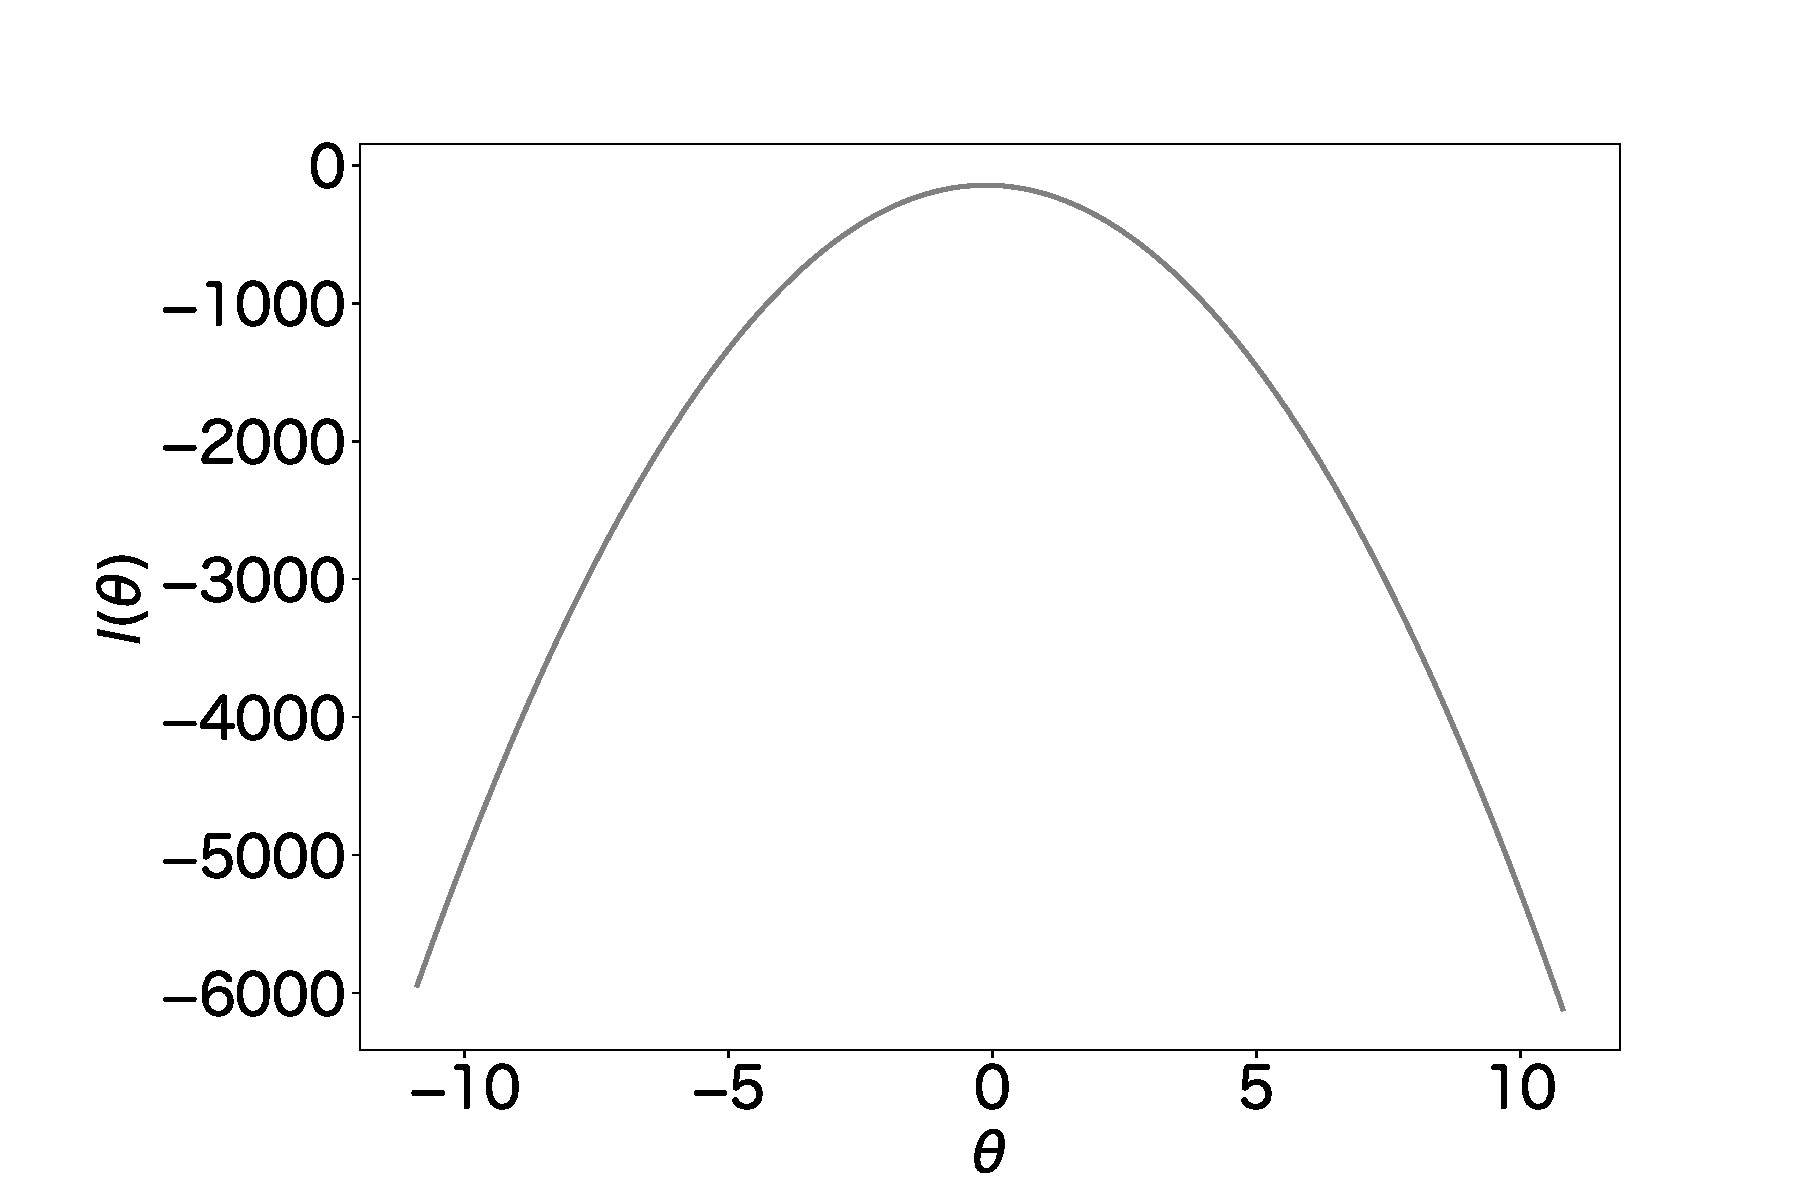
\includegraphics[width=15cm]{./image/02_/loglikelihood_function.pdf}
    \caption{$N(\theta,1)$における対数尤度関数。確率変数は、$N(0,1)$からサンプリングした。}
    \label{fig:loglikelihood_function}
\end{figure}

\subsection{最尤推定}
\begin{defi}
    尤度関数$l(\theta)$を最大にする$\theta$を最尤推定量という。
\end{defi}
正規分布における最尤推定量を計算してみる。正規分布は、母数を二つ持つので、尤度関数も2変数関数である。
まず、対数尤度関数は、
\begin{equation*}
    l(\mu,\sigma^2) = -\frac{n}{2}\log(2\pi\sigma^2)-\frac{1}{2\sigma^2}\sum_{i=1}^n(x_i-\mu)^2 
\end{equation*}
$l(\mu,\sigma^2)$を$\mu$で微分する。
\begin{equation*}
    \frac{\partial l(\mu,\sigma^2)}{\partial \mu} = \frac{\sum_i(x_i-\mu)}{\sigma^2}
\end{equation*}
$\frac{\partial l(\mu,\sigma^2)}{\partial \mu} = 0$とおいて、$\mu$について解くと、
\begin{equation*}
    \mu_{ML} = \frac{\sum_i x_i}{n}
\end{equation*}
これが最尤推定量となる\footnote{最尤がmaximum likelihoodなので頭文字を取ったMLを$\mu$の足に書いて$\mu_{ML}とした$}。
%言い換えれば、最尤推定量

同様に$\sigma^2$に関する微分を行う。
\begin{equation*}
    \frac{\partial l(\mu,\sigma^2)}{\partial \sigma^2} = -\frac{n}{2\sigma^2}+\frac{1}{2\sigma^4}\sum_i(x_i-\mu)
\end{equation*}
これが$0$と等しいとき、$\sigma^2$について解く。
\begin{equation*}
    \sigma^2_{ML} = \frac{\sum_i(x_i-\mu)^2}{n}
\end{equation*}

最尤推定量は、分布関数によって異なるので、計算してみるとよい。

\subsection{AIC(an information criterion)}
確率分布から対数尤度を求め、対数尤度の低い確率分布は、その中で相対的にデータに対して当てはまりの良い確率分布であると考えることができる。
最尤推定量を使った確率分布関数は、データを使って分布関数を決定しているので、データを使わずに求めた分布よりも、データに対して良い分布関数になりがちである。
そこで、対数尤度に対して罰則項を加えたAICを使って、データに対する当てはまりの良さを計算することがある。
\begin{equation*}
    AIC = -2\log f(x|\theta)+2k
\end{equation*}
ここで、$k$はデータによって決まったパラメータの個数である。

\subsection{マトリョウシカになったモデル}
複数のパラメータにより決定されるモデル$M(\alpha,\beta,\gamma,\omega)$がある。
このパラメータの中からモデルに影響を与えないように値を個体したモデル$M(\alpha,\beta,\gamma)$や$M(\alpha,\beta,\omega)$や$M(\alpha)$などが構成できることがある。
このようにパラメータの個数が少なくなったモデルを元のモデルからネストされたモデルや入れ子になったモデルと呼ぶことがある。
また、元のモデル$M(\alpha,\beta,\gamma,\omega)$を「フルモデル」と呼ぶ。

モデル$M(\alpha,\beta,\gamma)$をフルモデルとしたとき、$M(
\alpha,\beta)$はネストされたモデルでるが、$M(\alpha,\omega)$はネストされたモデルではない。


\chapter{数理統計の補足}

\section{正規分布の検定1}

また、母数分散$\sigma$について次が成り立つ。
\begin{theo}\label{normal_sigma_chi2}
    $X_1,X_2,\cdots,X_n \sim N(\mu,\sigma^2)$について、次が成り立つ。
    \begin{equation*}
        Y = (n-1)(\frac{S_x}{\sigma})^2 \sim \chi^2_{n-1}
    \end{equation*}
    ここで、$S^2_x=\frac{1}{n-1}\sum_{i=1}^n(x_i-\bar{x})^2,\bar{x}=\frac{1}{n}\sum_{i=1}^n x_i$である。
\end{theo}


%https://ds.machijun.net/clear-exercise-of-statistics/%E7%AC%AC7%E7%AB%A0-%E6%8C%87%E6%95%B0%E6%AF%8D%E9%9B%86%E5%9B%A3ex%CE%BC%EF%BC%89%E3%81%AE%E6%AF%8D%E5%B9%B3%E5%9D%87%E3%81%AE%E4%BF%A1%E9%A0%BC%E5%8C%BA%E9%96%93%E3%81%A8%E6%A4%9C%E5%AE%9Ap128/

\section{指数分布を含むモデル}

\begin{theo}
    $x_1,x_2,\cdots,x_n \sim Ex(\lambda)$とする。
    $x_1+x_2+\cdots+x_n \sim \gamma(n,\lambda)$である
\end{theo}

$n$を自然数とし、ガンマ分布$Ga(\frac{n}{2},2)$を特に、カイ2乗分布といい、$\chi ^2_n$で表す。

\begin{theo}
$n$を自然数とする。$G\sim\Gamma(\frac{n}{2},\beta),Y_n\sim \chi^2_n$とすると、$P(G\leq w) = P(Y_n \leq 2\beta w)$
\end{theo}
\begin{proof}
$w >0$に対して、
\begin{eqnarray*}
    P(G \leq w) &=& \int_0^w \frac{\beta^\frac{n}{2}}{\Gamma(n/2)}x^{n/2-1}\exp{(-\beta x)}dx \\
    &=&\int_0^{2\beta w} \frac{\beta^{\frac{n}{2}}}{\Gamma(n/2)}\left( \frac{t}{2\beta} \right)^{n/2-1}\exp{(-\beta t/2\beta)}\frac{dt}{2\beta} (x=t/(2\beta)) \\
    &=& \int_0^{2\beta w} \frac{1}{2^{n/2}\Gamma(n/2)}t^{n/2-1}\exp{(-t/2)}dt\\
    &=&P(Y_n \leq 2\beta w)
\end{eqnarray*}
\end{proof}

以上より$n\bar{x}\sim \Gamma(n,\lambda)$である。
このとき、$\lambda$の信頼区間を求める。$\lambda$の下限は、
\begin{equation}
    P(G\leq n\bar{x}) = \frac{\alpha}{2}
\end{equation}
を満たし、$\lambda$の上限は、
\begin{equation}
P(G\leq n\bar{x}) = 1-\frac{\alpha}{2}
\end{equation}
を満たす。
下限の式を変形していく。
\begin{eqnarray*}
    \alpha/2 &=& P(G\leq n\bar{x})  \\
    &=& P(Y_{2n}\leq 2n \lambda_l \bar{x})\\
    &\rightarrow& 2n\lambda \bar{x} = \chi^2_{2n}(1-\alpha/2)\\
    &\rightarrow& \lambda = \frac{\chi^2_{2n}(1-\alpha/2)}{2n\bar{x}}
\end{eqnarray*}
上限についても同様に、
\begin{eqnarray*}
    1-\frac{\alpha}{2} &= & P(G\leq n\bar{x}) \\
    &=& P(Y_{2n}\leq 2n\lambda \bar{x})  \\
    &\rightarrow& 2n\lambda \bar{x} = \chi^2_{2n}(\alpha/2)\\
    &\rightarrow&  \lambda = \frac{\chi^2_{2n}(\alpha/2)}{2n\bar{x}}
\end{eqnarray*}
以上によって、$\frac{1}{\lambda}$の信頼区間は、
\begin{equation}
    \label{exp_model_confidence_interval}
    \frac{2n\bar{x}}{\chi^2_{2n}(\alpha/2)} \leq \frac{1}{\lambda} \leq \frac{2n\bar{x}}{\chi^2_{2n}(1-\alpha/2)}
\end{equation}



\subsection{2標本・指数分布}
$X_1,X_2,\cdots,X_n \sim i.i.d Exp(\theta_1),Y1,Y_2,\cdots,Y_n \sim i.i.d Exp(\theta_2)$とする。帰無仮説$H_0$を、$H_0:\theta_1=\theta_2$とし、対立仮説$H_1$を、$H_1 : \theta_1 \neq \theta_2$とする。帰無仮説のもとで、尤度関数$L_{H_0}$は、

\begin{equation}
    L_{H_0} = \theta^{-n_1-n_2}\exp\{-\theta^{-1}T\}
\end{equation}
ただし、$T=\sum_{i=0}^n X_i+\sum_{i=0}^n Y_i$である。$\frac{\partial H_0}{\partial\theta}=0$となる$\theta$は、

\begin{equation}
    \frac{\partial H_0}{\partial\theta} = \{ -(n_1+n_2)+\theta^{-1}T \}\theta^{-n_1-n_2-1}\exp(-\theta^{-1}T).
\end{equation}
より、$\theta_0=\frac{T}{n_1+n_2}$である。
$\theta_0$を$L_{H_0}$に代入すると、
\begin{equation}
    L_{H_0} = \theta_0^{-n_1-n_2}\exp(-n_1-n_2).
\end{equation}

同様に、対立仮説のもとで、尤度関数$L_{H_1}$は、
\begin{equation}
    L_{H_1} = \theta_1^{-n_1}\exp(-\frac{n_1}{\theta_1}\bar{x})\theta_2^{-n_2}\exp(-\frac{n_2}{\theta_2}\bar{y})
\end{equation}
$\frac{\partial H_1}{\partial\theta}=0$となる$\theta_1$を計算する。
\begin{equation}
    \frac{\partial H_1}{\partial\theta_1}=\{ -n_1\theta_1^{-n_1-1} \exp(-\frac{n_1}{\theta_1}\bar{x})+n_1\bar{x}\theta_1^{-n_1-2}\exp(-\frac{n_1}{\theta_1}\bar{x})\}\theta_2^{-n_2}\exp(-\frac{n_2}{\theta_2}\bar{y}).
\end{equation}
$ \frac{\partial H_1}{\partial\theta_1}=0$より、$(-n_1+n_1\bar{x}\theta_1^{-1})\theta_1^{-n_1-1}=0$より、$\hat{\theta}_1=\bar{x}$である。同様に、$\hat{\theta}_2=\bar{y}$。
以上によって、$L_{H_1}$は、
\begin{equation}
    L_{H_1}(\hat{\theta}_1,\hat{\theta}_2) = (\hat{\theta}_1)^{-n_1}\exp(-n_1)(\hat{\theta_2})^{-n_2}\exp(-n_2)
\end{equation}
である。

尤度比は、
\begin{eqnarray}
    \varLambda = \frac{L_{H_1}}{L_{H_0}} &=& \frac{ (\hat{\theta}_1)^{-n_1}(\hat{\theta}_2)^{-n_2} \exp(-n_1-n_2)}{ \theta_0^{-n_1-n_2}\exp(-n_2-n_2) }\\
    &=& \left(\frac{\theta_0}{\hat{\theta_0}}\right)^{n_1} \left(\frac{\theta_0}{\hat{\theta_1}} \right)^{n_2}
\end{eqnarray}
尤度比検定より、$-2\log \varLambda \sim\chi^2_1$である。

$Ga(\alpha,\beta)$について、以下が成り立つ
\begin{eqnarray}
    k X &\sim& Ga(\alpha,\beta/k) \\
    \frac{1}{k} X &\sim& Ga(\alpha,k\beta)\\
    \chi^2_{2n}&=&Ga(n,2) 
\end{eqnarray}
以上を使うと、
\begin{eqnarray*}
    n\bar{X} &\sim& Ga(n,\frac{1}{\lambda}) \\
    \frac{n}{2}\bar{X} &\sim&(\frac{n}{2},\frac{1}{\lambda}) \\
    \frac{n}{2\lambda}\bar{X} &\sim& Ga(\frac{n}{2},2)=\chi^2_{n}
\end{eqnarray*}
また、ガンマ分布とベータ分布の関係より、$X_1 \sim Ga(\alpha_1,\beta),X_2\sim Ga(\alpha_2,\beta)$ならば、$\frac{X_1}{X_1+X_2}\sim Beta(\alpha_1,\alpha_2)$である。以上より、
$Z=\frac{n\bar{X}}{n\bar{X}+m\bar{Y}}\sim Beta(n,m)$である。このことから、棄却域($z_1 \leq Z \leq z_2$)を求めることができる。具体的には、
\begin{equation}
    \int_0^{z_1}\frac{1}{B{n,m}}z^{n-1}(1-z)^{m-1}dz = \alpha/2,      \int_{z_2}^{\infty}\frac{1}{B{n,m}}z^{n-1}(1-z)^{m-1}dz = \alpha/2.
\end{equation}
この解$z_1,z_2$を計算すれば良い。






%https://stats.stackexchange.com/questions/81151/likelihood-ratio-for-two-sample-exponential-distribution
%https://stats.stackexchange.com/questions/81151/likelihood-ratio-for-two-sample-exponential-distribution


\subsection{中心極限定理}
中心極限定理は本書の内容を超えるので、あえて紹介を避けてきた。一般的な統計学の本には詳細が書かれているので、そちらを読んだ方が良い。
\begin{theo}[中心極限定理]
    期待値$\mu$と分散$\sigma^2$を持つ独立分布に従う確率変数列$X_1,X_2,\cdots$に対し、$S_n=\sum_{k=1}^nX_k$とおくと、
    $S_n$は、期待値$0$、分散$1$の正規分布に分布収束する。
\end{theo}

統計学のユーザーの中には、次のことが成立すると考えている\footnote{
    中心極限仮説が成り立つと考えている人は多い。
    \\ \url{http://www.ner.takushoku-u.ac.jp/masano/class_material/waseda/keiryo/R10_inference.html#3_%E4%B8%AD%E5%BF%83%E6%A5%B5%E9%99%90%E5%AE%9A%E7%90%86} .
    \\ \url{https://yukiyanai.github.io/stat2/clt.html}.
    }。
\begin{hypoth}[中心極限仮説]
    一般のデータについて、データのサンプルサイズを大きくすると、その平均$\bar{x}$は、$\bar{x}\sim N(\mu,\sigma^2/n)$。
\end{hypoth}
反例がすぐに出てくるので、このような仮説は一般には成り立たない。例えば、データがコーシー分布から生成されている場合、成り立たない。

少なくとも一人は、次のように考えていた。
\begin{hypoth}[中心極限仮説2]
    サンプルサイズを大きくすると、正規分布に近づく。
\end{hypoth}
これも間違いである。中心極限定理の前提のもと、標本平均を集めると正規分布に近づくことはありえる。


\if 0
\subsubsection{ サンプルサイズが大きくなるとデータの構造がわかる}
サンプルサイズが増えると、正規分布を仮定できると書いてある文献もあるが、これは大数極限定理が成立する状況に限られるので、一般の母集団の特徴は正規分布を仮定した統計モデルで捉えるられるとは言い切れない。


サンプルサイズが増えることの利点として、おおよその分布の形がわかるということが挙げられる。
分布の形がわかれば、尤度ひを使った検定が可能になり、棄却すべき統計モデルがわかるようになる。
このことは、研究をさらに進めるさいに、どのような統計モデルを構築すれば良いのかの指針となりうる。
もう一つ利点をあげるなら、比較したい分布との違いを表示することで明らかにできるという点である。
言い換えると、少数のサンプルサイズのときに検定を使うことで、統計モデルの母数を検定することに意味があったのだが、
サンプルサイズが大きくなることで、プロットすれば分布の形の違いが現れるので、検定する意味がなくなる。
\fi

\if 0
信頼区間が狭くなるというふうに書いてあることもあるが、これも正しくないはず。
Cauchy分布を使って確かめてみる。
\fi 


\if 0
一方で、データの分布形を判断しようという意見も当然出ている。
\url{https://www.shindanyaku.net/statistics/vol_05/index.php}
\fi 

\if 0
統計学では、あえてデータが正規分布しているという統計モデルを設定し、その統計モデルを使って推測を行います。

https://www.ncchd.go.jp/press/2017/adultheight.html
https://jech.bmj.com/content/71/10/1014.long

\fi 

%
\chapter{仮説検定の3つの枠組み}
現在利用されている仮説検定の枠組みを紹介する。
それぞれの枠組みは前提が異なっており、それぞれの問題で良い推測を与える。
適切な枠組みを選ばなければ間違った解釈をしてしまう事になる。
我々の行なっている科学では、F型の枠組みを使う。
以降の章では、F型の問題について考える。



\begin{SMbox}{有意性検定・仮説検定}
    Fisherは、帰無仮説を設定し、帰無仮説とデータを比較検討する方法を構築した。これを、有意性検定という。これに対して、Neyman-Pearsonらは、帰無仮説に加えて、対立仮説を設定し、データを元に帰無仮説を棄却するかの判断を有意水準により行う意思決定の枠組みを構築した。これを、仮説検定と呼ぶことがある\cite{1573106361610039296}。
    現代の科学の多くは、FisherとNeyman-Pearsonの両方を組み合わせ、帰無仮説・対立仮説を設定し、帰無仮説とデータの乖離を$p$値によって調べ、棄却するかを検討する。ここでの$p$値は、Neyman-Pearsonの解釈から、20回に1回程度のことを有意と呼ぶことにしている。
    この流派をハイブリッド仮説検定法\cite{published_papers/18436201}と呼ぶことにする。
        %有意性検定を統計学\cite{upton2010統計学辞典,2009数理統計ハンドブック}や数学\cite{日本数学会2007岩波数学辞典}の辞書で調べたが、該当する言葉は見つからなかった。一方で、仮説検定は統計学\cite{upton2010統計学辞典,2009数理統計ハンドブック}などの辞書でも見つけることができた。
        %この言葉の使い方は、\cite{鳥類学における統計学_2018}に乗っていた。
\end{SMbox}



\section{F型}
F型では、既存の研究結果からモデルを構築し、そのモデルによりある集団の性質が予測できるかを調べる。
その後、計測結果を元に、その集団を予測できそうなモデルを構築する。
次の実験では、構築したモデルを利用し、予測が可能かを調べていく。
または、同じ集団についてさまざまな計測を行い、予測性能をあげるようにモデルを構築する。

\subsection{解決できる問題} 




\section{NP型}
NP型では、すでに前提になっていることから著しく外れたことが起きたことを検出するための方法である。
言い換えるなら、まず、何度も計測を行い、モデルが事象をよく予測できるようにモデルを構築する。
そして、母集団から無作為抽出し、標本を得る。
最後に、標本の統計検定量がモデルの予測を著しく外れているならば、
これまで計測していた現象が得られので、前提となる計測または母集団が変化したと疑う。

\subsection{解決できる問題}
NP型で扱う問題をいくつか挙げる。
\begin{quote}
    ある調味料の製造ラインでは, 砂糖の含有量 (g) は, 原料の不均一や製造ラインの狂いなどから変動するが, 標準偏差は常に一定で$\sigma=3$ の正規分布に従っているとしてよい. 各製品の砂糖の含有量が$\mu=60$になるように調整してラインを稼働させて, しばらくしてから, $25$個の製品を抜取検査したところ, 砂糖の含有量の平均値は$\bar{x}=61.63$であった. その時点で製造ラインは$\mu=60$を保持していると言えるだろうか.

    %\\ https://www.math.is.tohoku.ac.jp/~obata/student/subject/file/2019-EStat-All.pdf
\end{quote}
正規モデル$M(60,3^2)$によって予測ができるという前提条件を満たしている。この前提を元に、無作為抽出した$25$個がそのモデルにより予測できるのかを調べる。標本全体とモデルの累積分布などを比較する方法もあるが、ここでは、検定によって調べてみる。このモデルでは、
\begin{equation*}
    Z=\sqrt{n}\frac{\mu-\bar{x}}{\sigma} \sim N(0,1)
\end{equation*}
である。変数を入れれば、$Z=2.72$となる。$\varPhi(Z)<\varPhi(1/20=0.05)$であり、モデル内で、20回に1回よりも少ない頻度で観測されないようなことが現実で起きている。
または、$\varPhi(Z)<\varPhi(2\sigma=2)$であり、$2\sigma=2$(標準正規分布の中で)よりも珍しいことが起きているので、モデルでの予測ができないことが起きている。
偶発的に生じた可能性も捨てられないが、製造過程に不具合が生じているのではないかと推測される。



\subsection{解釈}

%NP型の問題では、前提が守られていることを確認できる状況においてのみ使える。
%言い換えれば、何度も何度も繰り返しモデルと現象を比較した結果、モデルが現象をよく予測できるということが確かめられているということである。
%頻度論で明らかになった数学を全て使うことができる。

\section{ハイブリッド型}
\subsection{解決できる問題}


%\chapter{モデルを使った有意性検定}

\section{モデルの設定}
帰無仮説$\mu=\mu_0$をを含む統計モデル$M(\mu_0)$を帰無モデル($M_{H_0}$)、対立仮説$\mu\neq \mu_0$を含む統計モデル$M(\mu\neq\mu_0)$を対立モデル($M_{H_1}$)と呼ぶ。
一般に、統計モデルの否定したい母数$\mu_0$を帰無仮説と言い、その母数ではないという$\mu\neq\mu_0$を対立かせつと言います。つまり、次のように帰無仮説を含む統計モデル$M_0$を構築します。

具体的には、データがある特定の母数$\mu$をもつ統計モデルの信頼区間に含まれるか否かによって、統計モデルが棄却されるかを調べます。
\begin{itemize}
    \item i.i.d
    \item 数学関数
    \item 統計モデルの母数を$\mu$とし、$\mu=\mu_0$
\end{itemize}
一番最後の仮説が帰無仮説と言います。
対立仮説を含む統計モデル$M_1$は、$M_0$と同様の仮説(1),(2)から構成されますが、仮説3は統計モデル$M_0$と$M_1$で異なります。
\begin{itemize}
    \item i.i.d
    \item 数学関数
    \item 統計モデルの母数を$\mu$とし、$\mu\neq\mu_0$
\end{itemize}
一番最後の仮説が対立仮説です。$M_1$の最後の仮説は、$M_0$の最後の仮説の否定系になります。

二つの統計モデルを作って、$M_0$で計算される信頼区間に、データから得られる統計量が入らないなら、$M_0$は棄却されます。逆に、統計量が信頼区間に入るなら、何も起こりません。
このように、否定したい仮説を設定し、少なくとも帰無仮説を含む統計モデルはだめだったと判断します。

 %これは消そう
\chapter{仮説検定の実際}
実際に利用されている仮説検定について説明する。ここではあえて間違っているとされる方法も含めている。

正しい仮説検定について説明してある論文は多い。それらの中でも、数学は同じだが、手順には差異がある。


\section{仮説検定における前提}
仮説検定とは、仮説を採用するかを決定する方法である。数多くの研究で、科学的な検証がなされたことを示すために、仮説検定が利用されている。

その手順は、データの出現頻度を予測するという方法論を十分に利用しきれていない\footnote{予測を一切考えないので、モデルという考えが存在しないように見える}。
%私が、仮説検定を行うことはない。

%Fisherが有意検定を提案した後に、Neyman-Pearsonが仮説検定を提案し、その後、それらを組み合わせた仮説検定が利用されることになった。

科学的仮説検定では、データが統計的法則により予測可能であるかを示すため、モデルを構築した。
仮説検定では、モデルの代わりに仮説を使う。モデルの母数に関する仮説のみを帰無仮説と定義し、帰無仮説で指定した母数ではないを対立仮説と呼ぶ。
帰無仮説の元、標本の統計量以上に偏った値が得られる確率($p$値)を計算する。
$p$値が$0.05$よりも小さいならば、対立仮説を採択し、$p>\alpha$ならば判断を保留する。

仮説検定の枠組みでは、データが前提を満たさなければならないと考えられていることが多い\footnote{仮説検定を使う研究者にとって、モデルを使った予測であるということは意識されない。モデルの仮定ではなく、仮説検定をするための前提のことである}。
例えば、データは独立同一の分布関数から得られている\footnote{これを確かめる方法はあるのだろうか。言い換えるなら、現象が数学的分布関数により生じていることを確かめる必要がある}。また、正規分布を仮定しているのであれば、データの分散と帰無仮説の分散が等しいなどである。
そのため、仮説検定を行う前に、いくつかの仮説検定を行い、これらの前提を確かめる。正規分布の仮定は、$Shapiro$検定を使う。その後、正規分布であれば、等分散検定などを行う。
これらの前段階の検定では、$p$値が設定した$\alpha$よりも小さければ、対立仮説を採択し、$p>\alpha$であれば、帰無仮説を採用する\footnote{検定により対立仮説や帰無仮説を採択することはできないが、仮説検定においてはできるという立場をとる。}\footnote{検定ではモデルを決定できない。仮説検定においてはそれができるということにして、仮説の論証がなされている。}\footnote{採択すると言い切ったが、前段階の検定においては、採択または棄却と判断してるといっておいた方が現状にあっている。}。
さらに、最終的な仮説検定においては、$p<\alpha$ならば帰無仮説を棄却し、$p>\alpha$ならば、判断を保留する
\footnote{仮説検定の手順は分野によって少しずつ異なるので、指導教員に手順を聞くことを勧める。留年したくないなら、魔術を信仰した方が良い。やれと言われたことをやらなければ論文は通らない。}
\footnote{科学的仮説検定と仮説検定には互換性がない。前者は、モデルとデータの乖離を検討するという考えである、後者は仮説が検証できると盲信し、検証する方法である。}
\footnote{複数回の検定を行うので、多重検定の問題もあり、想定された$\alpha$水準を満たされないことが指摘されている。}
\footnote{仮説検定が廃止されたとしても、過去の研究においては仮説検定が使われており、それら過去の研究を理解する必要がある。この理由から仮説検定を理解しなければならない}。



\begin{SMbox}{p値の解釈}
$p$値は分野によって多様な解釈がなされることがある\cite{published_papers/18436201,2020医療統計解析使いこなし実践ガイド}。
\if 0
例えば、ASAの声明[\cite{ASA_JA}]を引用しているにもかかわらず、
$p$値は、証明したい仮説が真である場合、研究で行った前提条件が担保されている場合、研究で得られた結果が実際に得られる確率を示している\cite{2020医療統計解析使いこなし実践ガイド}。

などと書かれる場合がある。
ここで、「実際に得られる確率」が何を指しているのかが不明確であるが、「統計モデル上で実験で得られた統計量が得られる確率」を意図すると読み替えることはできるのだろうか。
\fi

よい解釈として以下の6つの原則が示されている\cite{published_papers/18436201}
\begin{enumerate}
    \item $p$値はデータと特定のモデルが矛盾する程度を示す指標の一つである。
    \item $p$値は調べている仮説が正しい確率や、データが偶然飲みで得られた確率を図るものではない。
    \item 科学的な結論や、ビジネス、政策における決定は$p$値がある値を越えたかどうかのみに基づくべきではない。
    \item 適正な推測のためには、全てを報告する透明性が必要である
    \item $p$値や統計的優位性は、効果の大きさや結果の重要性を意味しない。
    \item $p$値は、それだけでは統計モデルや仮説に関するエビデンスの、よい指標とはならない。
\end{enumerate}

\if 0
    $p$値や信頼区間を報告することがASAの声明では求められている。私は、それら以外の情報として、ランダムサンプリングされているということ・再現可能性・正規分布を含んだ統計モデルなどを研究者がどの程度信じているのかということも報告するべきだと考えている。統計モデルの仮定が現象から著しく外れているのならば、統計モデルを使った推論は無意味である。
    また、研究者の統計学への心情がわかれば、報告に価値があることを理解しやすくなる。
\fi 
\end{SMbox}
\begin{SMbox}{p値への誤解}
    誤解とされる解釈はも引用しておく\cite{idiot_statistics2014}\footnote{原典は\cite{GOODMAN2008135}である。孫引き引用である}。
    以下の解釈は、統計ユーザーの流派によらず間違いであるとされることが多い\footnote{これらの誤解を採用している科学者もいないとは言えない。教科書でも誤解を広めていることがある}。
    \begin{enumerate}
        \item $p=0.05$ならば、帰無仮説が真である確率は$5\%$しかない。
        \item $p\geq 0.05$のような有意でない結果は、グループ間に差がないことを意味する
        \item 統計的に有意な発見は客観的に重要である
        \item $p$値が$0.05$より大きい研究と小さい研究は矛盾する
        \item $p$値が同じ研究は帰無仮説に対して同等の証拠を提供する。
        \item $p=0.05$は、帰無仮説のもとで$5\%$しか起こり得ないデータを観察したことを意味する
        \item $p=0.05$と$p\leq 0.05$は同じことである。
        \item $p$値は不等式の形で書かれるものである(例えば、$p=0.015$のときは$p\leq 0.02$とする)。
        \item $p=0.05$は、帰無仮説を棄却したとしたら、第一種の誤りの確率が$5\%$しかないことを示す。
        \item 有意水準$p=0.05$のもとで、第一種の誤りの確率は$5\%$になる。
        \item ある方向を向いた結果やその方向の結果があり得ない差異を気に留めないのであれば、片側の$p$値を用いるべきである。
        \item 科学に関する結果や処方の方針は$p$値が有意であるかどうかに基づくべきである。
    \end{enumerate}
\end{SMbox}


\begin{SMbox}{モデルの仮定を満たせるのか}
    \ 
    \begin{quote}
    最初の原則。最初に述べられている原則ですが、P値はデータと特定の統計モデルが矛盾する程度を示す指標の一つであるというふうに書かれています。ここでですね、統計モデルは何かって言うと、統計モデルは必ず一連の仮定のもとで構成されています。どんな仮定かと言いますと、統計の教科書をみますと、「データが正規分布している」とか、「平均値が等しい」などが統計モデルに必要な仮定とされているのですが、まず、一番大切なことは、データを撮るときに、先程の試験のように、薬剤のランダム割り当てが行われているとか、対象者を剪定するときにランダムサンプリングがなされているか、こういったことも統計モデルの仮定に含まれています。
    それから当然、研究計画がきちんと守られているかも統計モデルが必要とする前提の一つです。例えば、先程の臨床試験で言えば、
    結果の解釈も変わってきます。最後まで対象者が追跡できているのか。追跡不能とからつだくがあったとすると、統計モデルの後世に影響を与えます。もちろん解析方法も妥当な結果を与える解析方法でなければいけない。
    こういったことを満たしていなければ、統計モデルの仮定を満たしているとは言えない。
    %もちろん、全ての解析結果が報告されている。これは統計モデルに必要な仮定とは言えないですが・・・
    \footnote{京都大学大学院医学研究科 聴講コース 臨床研究者のための生物統計学「仮説検定とP値の誤解」佐藤 俊哉 医学研究科教授 \url{https://www.youtube.com/watch?v=vz9cZnB1d1c} }
    \end{quote}

    この意見は統計モデルに関する仮定と実験計画の二つの要素が混じっている。実験計画を統計モデルの仮定を満たすように設計するという意見だと考えられる。
    私はこの意見に賛成しない。

     まず、統計モデルの仮定が自然において満たされていることはほとんどない。また、「平均値が等しい」という仮定であるが、ある平均値をもつ統計モデルとデータを比べるさいに、データの平均値が異なる場合においても、統計モデルを使ってそのデータの出現頻度などを推定することが可能である。
     このことは、モデルの仮定をデータが満たさなければならないことを示唆していない。

     次に、実験計画については、科学者がみたい効果を見るために設定しているのもである。ランダムサンプリングしているのは、対象に偏りがないようにし、さまざまな対象で効果があるかを検証するためである。対象の選定に偏りがあった場合、本当に推測したかったことが推測できない。例えば、成人以上を対象にした試験なのに、60歳だけしかからサンプリングできなかったなら、成人に対しての言及はできない。
     これらのことは、モデルに対してではなく、科学者がみたいものが見れなくなることを意味する。

\end{SMbox}



\if 0
p値が小さいとき、統計モデルの少なくとも一つの仮定と実際のデータとが合わないことが考えられます。そこでまず、統計モデルの仮定を満たしているのかを確認します。統計モデルの仮定(1)を確認します。身長データを無作為抽出して計測したため、身長データはそれぞれ独立であると考えられます。次に統計モデルの仮定(2)です。これは、Q-Qプロットを使います。もし、データが正規分布ではなさそうであれば、この統計モデルは使えません。
以上のことが確かめられたら統計モデルの仮定(3)が実際のデータと異なると結論付けます。少なくとも、ある母数では実際のデータと乖離していると主張するわけです。
\fi

%\section{科学的仮説検定}

\if 0


この手順を身長の検証をするためになぞってみます。
\begin{enumerate}
    \item 普段の観察から、身長はある平均値の周りに対象に分布していることがなんとなくわかっているので、対象な分布関数の中から関数を選ぶ。また、サンプルサイズが大きいときの標本を見ると、正規分布でよく推定できることが知られている。以上のことから、正規分布で推測を試みる。
    \item 次の統計モデルを構築する。
    \begin{quote}
        \begin{itemize}
            \item 確率変数は独立同一分布に従う
            \item 正規分布関数
            \item 正規分布関数の母数$\mu,\sigma=5.7$
        \end{itemize}
    \end{quote}
    \item $\mu=170$
    \item 次のことがわかっている$x_1,\cdots,x_n$が正規分布$N(\mu,\sigma^2)$に従う確率変数であるならば、$\frac{\bar{x}-\mu}{\frac{\sigma}{\sqrt{n}}}\sim N(0,1)$である。ここで、$\bar{x}=\frac{x_1+x_2+\cdots+x_n}{n}$
    \item $\alpha=0.05$
    \item 母数からサンプルをランダム抽出し、標本とする。
    \item 無作為抽出できていかたと、標本を正規分布で推測しても良さそうかを検証する
    \item 標本の平均$\bar{X}$を計算し、統計モデルでの出現頻度を計算する。
    \item $p<\alpha$ならば、統計モデルの仮定のうち少なくとも一つがデータと乖離していると考える
    \item 仮説(1),仮説(2)はそれほど悪くない仮説であると思われるので、母数に関する仮定が間違っていると考えられる。以上から、母数は$\mu$ではないと宣言する。
\end{enumerate}

もしも、予備実験から実験状況に変化がなければ、帰無仮説を含んだ統計モデルは棄却されにくい。実験状況に変化があれば、帰無仮説を含んだ統計モデルは棄却されやすくなる。


\fi






\if 0 

このとき、$Z(\bar{x},\mu)$が$N(0,1)$においてよくある値でない場合に、棄却します。
一方で、$Z(\bar{x},\mu)$が$N(0,1)$においてよくある値だったとしても、統計モデルを採用するとは言いません。
また、$Z(\bar,\mu)$の絶対値が$0$よりも十分大きな値を取れば、$N(0,1)$において出にくいということがわかります。これは、$|\bar{X}-\mu|$つまり、統計モデルの母数$\mu$と平均値$\bar{X}$の絶対値が大きければ、$Z(\bar{X},\mu)$の出現頻度は低く、絶対値が十分$0$に近ければ、$Z(\bar{X},\mu)$の出現頻度は高いことを意味します。

ここまでは、全て数学的フィクションである統計モデルの話をしました。では、現実のデータが
では、p値が語っていることを考えるいきます。


以上のことから、この検定を使うには、少なくともQ-Qプロットが必要であることが分かります。


一般に、統計モデルが棄却されない母数の領域を信頼区間といい、棄却される母数の領域を棄却区間という。
特に、$p=0.05$を基準とし、その基準における統計モデルが棄却されない区間を$95\%$ ($100*(1-0.05)$)信頼区間という。


信頼区間と対応する言葉として、採択域(棄却域)というものがある。棄却域は、確率変数を標準正規分布へ変数変換した後での信頼区間である。これは明らかに信頼区間と一対一対応する。

https://twitter.com/genkuroki/status/1270179975195316224


信頼区間は、データによって棄却されない母数の範囲のことである。

信頼区間は、統計モデルが棄却されるパラメータかどうかを表しているので、現実の推論を全く行っていない。

身長を統計モデルにより扱うことで、$p<0.05$では帰無仮説が棄却され、推測を行う統計モデルとはいまいちだということは分かったと思う。一方で、$p>0.05$となった場合でも積極的に採択しないことはなぜだろうか。次は、その理由を探る。
\fi



\if 0
\begin{SMbox}{統計モデルを積極的に採用しない理由}
設定した$\alpha=0.05$よりも大きな$p$値をもつ統計モデル$M(162.2)$は、それなりに推測するでしょうか。この統計モデルにより$P(x=170)$は、極めて少数であり、サンプルサイズを大きくしたときと乖離していることが分かります。このことから、全ての現象に対して特定の$p$値を元に棄却するモデルを決めることの無意味さを感じることができます。
\end{SMbox}
\fi


\if 0    
\begin{SMbox}{帰無仮説のもとで偶然には起こり得ないことが起こった}
    帰無仮説のもとで偶然には起こり得ないことが起こったと言うふうに書くと、現実に起こりにくいと言うふうに印象付けられてしまう。
    非現実である統計モデルの上で、実験で得られた統計量以上の値が得られる確率は十分小さいと言い換えた方が良い。
\end{SMbox}
\fi


\if 0
\begin{SMbox}{正規分布を前提にできる場合}
TODO:意味不明\\
非常に限定された条件で、標本が正規分布していることを前提として使えます。具体的には、標本が分布関数(Cauchy分布は当てはまらない)により生成されていることが前提となる場合です。このとき、中心極限定理によって、十分なサンプルサイズがある場合には、データが正規分布に近づきます。
言い換えれば、サンプルサイズを増やしていけば任意に小さな$p$値を得ることができます。
一方で、一般の現象は特定の分布関数によってデータが生成されているとは言うことはできません。この場合、正規分布に近づくことが正当化できる科学理論はありません。     
\end{SMbox}
\fi


\if 0
\section{一般的な仮説検定の手順}
一般的な仮説検定の手順をまとめる。
%
\begin{framed}
    \begin{itemize}
        \item 帰無仮説($\mu = \mu_0$)・対立仮説($\mu\neq \mu_0$)を設定する。
        \item 仮説が正しいと考えたとき、検定統計量従う分布を考える(4)。
        \item $\alpha$を設定する。
        \item 母集団からの無作為抽出により標本を得る。
        \item 検定統計量を計算し、その出現する確率$p$値を計算する。それが$\alpha$以下であれば、$\mu=\mu_0$ではないと結論づける(帰無仮説が棄却された。)。%ただし、前段階検定においては、$p>\alpha$であれば、帰無仮説を採択する。
    \end{itemize}
\end{framed}
\fi

\section{仮説検定の手順}
仮説検定の手順を確認します。
仮説検定では、仮説の前提が正しいことを決定する必要がある。
これは、特定の分布関数にデータが従っていることを前提にし、前提が正しいならば、帰結も正しいと考えており、正しいデータを使わなければ仮説を検証できないと考えているからである\footnote{実際には、前提は検証できないのだが、仮説検定においては、できると決定されている}。%そのようなケースは実際の現象においては非常に稀であると考えられる。
ゆえに、データと想定した仮説の前提を満たしていることを注意深く検証しながら、仮説検定を利用することが求められている\footnote{科学的仮説検定では、現象を予測するためにモデルを使ったので、モデルの仮説をデータが満たさなくても良い}。
%統計モデルがデータと乖離していれば、推定値が何を意味するかが捉えられなくなると考えられており、
データが前提を満たすように、得られたデータを仮説の前提と一致するように、数学的な変換を施すこともある\footnote{標本分布の形が失われる}。
%科学的仮説検定では、モデルを調整し、再度計測することを要求
%ので、統計モデルの改訂を要求されることもある。
%ただし、$p$値を小さくすることを目標に統計モデルを改訂してはいけない。

\begin{framed}
    \begin{enumerate}
        \item 仮説検定が使える前提が何かを確認する。前提は以下のようになることが多い。
        \begin{quote}
            \begin{itemize}
                \item 確率変数は独立同一分布に従う
                \item 分布関数(正規分布など)
            \end{itemize}
        \end{quote}
        %\item 統計モデルに母数を設定する.経験的に知っている値や、過去の論文や予備実験で明らかになった値である方が良い
        %\item 統計モデルからサンプリングした確率変数の統計量が従う分布関数を探す。統計モデルの性質によって、母集団から得られた標本から得られた統計量の出現確率が計算可能になる。一般の仮説検定は本などでこの分布関数を確認する。
        \item 有意水準$\alpha$を設定する(さまざまな業界で$0.05$が設定される)。
        \item 母集団から無作為抽出を行い、標本を得る
        \item 標本が仮説の前提を満たしていることを確認する。標本分布と仮説の前提の分布関数がある程度一致していることを調べる。正規分布を前提にしているなら、正規分布の検定を行う。
        %\begin{quote}
            %標本が統計モデルにより推測できないと思われる場合、分布関数を変更し、統計モデルを再構築する。

            %または、母集団の性質が別の分布関数になったのだから、仮説検定を使うまでもなく、変化があったことが主張可能である。例えば、正規分布で推測できると(過去の実験や研究結果から)思われてたデータが、実際には指数分布的だった場合など。この場合、計測機器・無作為抽出の方法などに異常がなかったかも確認すべきである。
        %\end{quote}
        \item 標本から統計量を計算し、その値以上に大きな値をとる確率を計算する($p$値)。
        \item $p$値が$\alpha$以下であれば、帰無仮説を棄却し、対立仮説を採択する。
        \item $p$が$\alpha$以上であれば、判断を保留する(最終検定前の検定では採択する)。%\footnote{対立仮説を採択しない流派もあるが、採択していると考えるのが妥当である。}。
    \end{enumerate}
\end{framed}




\begin{SMbox}{第一の過誤・第二の過誤・統計モデルが正しい}
    Neyman-Pearson流の統計学においては、$\alpha,\beta$を次のように定義する。帰無仮説が正しいとき、誤ってそのモデルを棄却してしまう間違いを第一の過誤といい、この確率を$\alpha$とする。また、対立仮説が正しいのに、帰無モデルを採択する間違いを第二の過誤といい、この確率を$\beta$とする。

    %私は、ある統計モデルが正しいとは考えないので、「モデルが正しいとき、間違えてそのモデルを棄却する間違い」ということを考える流派に同意できなかった。
    %仮説は棄却されることはあるが、正しいことや積極的に採択されることは稀であるというのはFisherの流派が近い。
    %ただし、Fisherは、「$p$値を帰無仮説が正しいという条件のもとで、手元にあるデータ、およびさらに極端なデータが得られる確率」と定義した[\cite{1573106361610039296}]。
    %ここでの正しいという言葉の意図が重要である。
    %私は、「統計モデルの仮説が自然を記述するのにほどほど良いと考えられるとき、手元にあるデータの統計量以上の隔たりが統計モデル内で得られる確率」という意味であると捉え直し、科学的仮説検定を提案した。

    %Neyman-Pearson流派の統計学の教科書を科学の分野で見つけることができていない。
    %Fisher流派とNeyman-Pearson流派の両方を書いている教科書は存在しているが、「帰無モデルが正しい」とはどういうことかを答えたものを見つけることができていない。

    %Fisher流派とNeyman-Pearson流派の両方を同じように扱うことが問題視されることもある[\cite{published_papers/18436201}]。
\end{SMbox}



\begin{SMbox}{過誤の概念に対する懸念}
第一の過誤・第二の過誤に関する批判として\cite{norleans2004臨床試験のための統計的方法}がある。
\cite{2010毒性試験に用いる統計解析法の動向}において引用されていた部分を引用しておく。
%私も彼らの意見に同意する。
\begin{quote}
過誤の概念は非現実的である。根本的な問題は、我々が真実を知らないことである。現実の臨床試験では、我々は実験から学び、真実を知りたいと願うのであって、真実がすでに知られており、我々の観察を判断するのに利用できる、というようなものではない。現在利用できる情報だけに基づく決定は、それ以上の情報が利用できるときには間違っていたことがわかることもあり得る。それ以上の情報が得られないとき、決定を行なった元になる情報でその決定の評価を行うことは理論的に不可能である。一つの試験では、試験さそのものから得られる情報が、利用できる唯一の情報である。利用できる情報の調査と競合する利害の注意深いバランスを考慮した後でのみ、仮説の棄却や採択の判断が行われる。その後の試験の情報が利用できるようになるまでは、現在の判断が正しいか誤りかを判断する情報は存在しない。従って、一つの試験にとっては、過誤の考え方は全く意味を持たない。
\end{quote}
%何も考えず、$\alpha=0.05,\beta=0.8$としてサンプルサイズを
\end{SMbox}



%\section{何度も検定しよう}
% 塩野義製薬の薬
% https://mainichi.jp/articles/20220818/k00/00m/040/138000c
%https://www.mhlw.go.jp/stf/newpage_26901.html
%https://www.jstage.jst.go.jp/article/jjb/36/Special_Issue_2/36_S123/_pdf/-char/ja
% https://bio.nikkeibp.co.jp/atcl/news/p1/22/07/20/09735/
% https://twitter.com/penguin_pharm/status/1549746189561606144
% https://www.sankei.com/article/20220902-Y2DSR2RUWVM63G5QE6LS22VHEI/
% https://www.buzzfeed.com/jp/naokoiwanaga/s-217622?utm_source=dynamic&utm_campaign=bfsharetwitter
% https://www.kansensho.or.jp/uploads/files/guidelines/teigen_220902.pdf
% https://www3.nhk.or.jp/news/html/20220902/k10013800921000.html
% https://www3.nhk.or.jp/news/html/20220902/k10013800921000.html
% https://www3.nhk.or.jp/news/html/20220907/k10013806901000.html
% https://www.m3.com/news/open/iryoishin/1062171
% https://www.mixonline.jp/tabid55.html?artid=73353



\bibliography{ref} %hoge.bibから拡張子を外した名前
\bibliographystyle{junsrt}

\end{document}